%%%%%%%%%%%%%%%%%%%%%%%%%%%%%%%%%%%%%%%%%%%%%%%%%%%%%%%%%%%%%%%%%%%%%%%%%%%%%%%%%%%%%%%%%%%%%%%%%%%%%%%%%%%%%%%%%%%%%%%%
%CONFIGURATIÓN
%%%%%%%%%%%%%%%%%%%%%%%%%%%%%%%%%%%%%%%%%%%%%%%%%%%%%%%%%%%%%%%%%%%%%%%%%%%%%%%%%%%%%%%%%%%%%%%%%%%%%%%%%%%%%%%%%%%%%%%%
%:Clase del documento
\documentclass[paper=a4,10pt, Myfinal=true,twoside]{scrbook}
%, Myfinal=true, Minion=true, English=true




\usepackage{algorithmic}
\usepackage{color}
\usepackage{pdfpages} 
\usepackage{xcolor}
\usepackage{tcolorbox}
\usepackage{subfigure}
\usepackage{svg}
\usepackage{multirow}
\usepackage{ulem}
\usepackage{csvsimple}
\usepackage{makecell}
\usepackage{svg}
\usepackage{graphicx}
\usepackage{float}
\usepackage{csvsimple}
\usepackage{amsmath}
\usepackage{subfig}

% TFM

\usepackage{caption} % Para aumentar las opciones de diseño
\usepackage{csvsimple}


%:Paquete de estilos propuesto
\usepackage{estiloLibro}

%:Paquete para notaciones específicas
\usepackage{estiloNotacion}

%:Paquete para incorporar aspectos concretos de la edición
\usepackage{estiloPortada}

\usepackage{tabularx,booktabs}

%:Para modificar fácilmente la fuente del texto. 
\makeatletter
\ifdtsc@Minion % Queremos utilizar la fuente Minion y lo hemos declarado al principio
	\ifluatex
		\setmainfont[Renderer=Basic, Ligatures=TeX,	% Fuente del texto 
		Scale=1.01,
		]{Minion Pro}
   		% En este caso conviene modificar ligeramente el tamaño de las fuentes matemáticas
		\DeclareMathSizes{10}{10.5}{7.35}{5.25}
		\DeclareMathSizes{10.95}{11.55}{8.08}{5.77}
		\DeclareMathSizes{12}{12.6}{8.82}{6.3}
%		\setmainfont[Renderer=Basic, Ligatures=TeX,	% Fuente del texto 
%		]{Adobe Garamond Pro}
%		\setmainfont[Renderer=Basic, Ligatures=TeX,	% Fuente del texto 
%		]{Palatino LT Std}
	\fi
\else
	\ifluatex
		% Para utilizar la fuente Times New Roman, o alguna otra que se tenga instalada
		\setmainfont[Renderer=Basic, Ligatures=TeX,	% Fuente del texto 
		Scale=1.0,
		]{Times New Roman}
	\else
		\usepackage{tgtermes} 	%clone of Times
		%\usepackage[default]{droidserif}
		%\usepackage{anttor} 	
	\fi
\fi
\makeatother

% Ejemplo de Glosario
\newacronym[type=main]{EPS}{EPS}{Escuela Politécnica Superior}
\newacronym[type=main]{UA}{UA}{Universidad de Alicante}

\makeindex
\makeglossaries %Si no se quiere el glosario, comentar esta línea.

%TAMAÑO LIBRO O A4
%Para definir el tamaño del documento, hay que elegir uno de los siguientes y comentar el otro
%Formato Libro
\geometry
{paperheight=250mm,%
paperwidth=180mm,%
top=25mm,%
headsep=7.5mm,%
footskip=10mm,%
textheight=190mm,%
textwidth=124mm,%
bindingoffset=15mm,%
twoside
}

%\usepackage[a4,center, cross]{crop}%para poner las cruces de esquina de página, poner la opción cross
% Formato A4
%\usepackage[paperheight=297mm, paperwidth=210mm, top=25mm, headsep=8.5mm, includefoot, textheight=240mm, textwidth=150mm, bindingoffset=0mm, twoside]{geometry}

%:Esquema de numeración por defecto
\setenumerate[1]{label=\normalfont\bfseries{\arabic*.}, leftmargin=*, labelindent=\parindent}
\setenumerate[2]{label=\normalfont\bfseries{\alph*}), leftmargin=*}
\setenumerate[3]{label=\normalfont\bfseries{\roman*.}, leftmargin=*}
\setlist{itemsep=.1em}
\setlength{\parindent}{1.0 em}

\setcounter{tocdepth}{2} % El nivel hasta el que se muestra el índice 






%%%%%%%%%%%%%%%%%%%%%%%%%%%%%%%%%%%%%%%%%%%%%%%%%%%%%%%%%%%%%%%%%%%%%%%%%%%%%%%%%%%%%%%%%%%%%%%%%%%%%%%%%%%%%%%%%%%%%%%%
%DOCUMENTO

%:Empieza el documento
\begin{document}
\thispagestyle{empty}
\begin{center}
	\begin{figure}[H]
		
\includegraphics[width=6cm]{figuras/logoua.jpg}
	\end{figure}
\end{center}
\vskip 2cm

\begin{center}
	{\large\titular{DEPARTAMENTO DE CIENCIA DE LA COMPUTACIÓN E INTELIGENCIA ARTIFICIAL} }
\end{center}
% Nombre de la facultad o escuela al que está adscrito.
\begin{center}
	{\large\titular{ESCUELA POLITÉCNICA SUPERIOR} }
\end{center}

\vskip 1cm
\begin{center}
	{\Huge\titular{Predicción de asistencia en accidentes de tráfico con un modelo de aprendizaje profundo}}
\end{center}
\textcolor[RGB]{170,170,170}{\rule{\linewidth}{4.2pt}}
\vskip 1cm
\begin{center}
	{\Huge\titular{Luis Pérez-Sala García-Plata}}
\end{center}
\vskip 1cm
\begin{center}
	{\normalsize\textbf{Tesis presentada para aspirar al grado de}}
\end{center}
\begin{center}
	{\large\titular{Doctor por la Universidad de Alicante}}
\end{center}
\begin{center}
	{\large\titular{Doctorado en Informática}}
\end{center}
\vskip 3cm
\begin{center}
	{\normalsize\textbf{Dirigido por:}}
\end{center}
\begin{center}
	{\large \titular{Dr. José F. Vicent Francés}}
\end{center}
\begin{center}
	{\large \titular{Dr. Manuel Curado Navarro}}
\end{center}
\clearpage
%:Construcción de la portada y hojas obligatorias. Ver edicionTesis.sty para posibles modificaciones
%\titulo{Medidas de Centralidad en Redes Urbanas Basadas en el Concepto del Vector Propio Dominante}
%\autor{Luis Pérez-Sala García-Plat}
%\director{José F. Vicent Francés y Manuel Curado Navarro}
%\titulodirector{Profesores Titulares}
%
%\departamento{Ciencia de Computación e Inteligencia Artificial}
%\centro{Escuela Politécnica Superior}
%\universidad{Universidad de Alicante}
%%\titulacion{Ingeniería Informática}
%\fecha{2024}
%\nombretrabajo{Tesis Doctoral}

%%%%%%%%%%%%%%%%%%%%%%%%%%%%%%%%%%%%%%%%%%%%%%%%%%%%%%%%%%%%%%%%%%%%%%%%%%%%%%%%%%%%%%%%%%%%%%%%%%%%%%%%%%%%%%%%%%%%%%%%
% PAGINA: PORTADA
%\portadaTesis{figuras/Fondo.jpg}

%:Para establecer características del pdf generado
\hypersetup
	{
 	linkcolor=ublue, %Tocar para poner color en enlaces
	pdfauthor={\elautor},
	pdftitle={\eltitulo}, 
	pdfkeywords={Formato de Tesis, Latex, EPS, Universidad de Alicante}	
	 }
%%%%%%%%%%%%%%%%%%%%%%%%%%%%%%%%%%%%%%%%%%%%%%%%%%%%%%%%%%%%%%%%%%%%%%%%%%%%%%%%%%%%%%%%%%%%%%%%%%%%%%%%%%%%%%%%%%%%%%%%

%:Todo lo que constituye la primera parte del texto que no es el cuerpo del texto en realidad
\frontmatter
\pagenumbering{Roman} %Pone la numeración en mayúscula (En español parece que es obligatorio)
%%%%%%%%%%%%%%%%%%%%%%%%%%%%%%%%%%%%%%%%%%%%%%%%%%%%%%%%%%%%%%%%%%%%%%%%%%%%%%%%%%%%%%%%%%%%%%%%%%%%%%%%%%%%%%%%%%%%%%%%
% PAGINA: DEDICATORIA
\dedicatoria{A .....} 
%%%%%%%%%%%%%%%%%%%%%%%%%%%%%%%%%%%%%%%%%%%%%%%%%%%%%%%%%%%%%%%%%%%%%%%%%%%%%%%%%%%%%%%%%%%%%%%%%%%%%%%%%%%%%%%%%%%%%%%%

%%%%%%%%%%%%%%%%%%%%%%%%%%%%%%%%%%%%%%%%%%%%%%%%%%%%%%%%%%%%%%%%%%%%%%%%%%%%%%%%%%%%%%%%%%%%%%%%%%%%%%%%%%%%%%%%%%%%%%%%
% PAGINA: AGRADECIMIENTOS
% !TEX root =../LibroTipoETSI.tex
\chapter*{Agradecimientos}
%\pagestyle{especial}
\pagestyle{empty}

Esta tesis es la memoria del camino de investigación .....


%%%%%%%%%%%%%%%%%%%%%%%%%%%%%%%%%%%%%%%%%%%%%%%%%%%%%%%%%%%%%%%%%%%%%%%%%%%%%%%%%%%%%%%%%%%%%%%%%%%%%%%%%%%%%%%%%%%%%%%%

%%%%%%%%%%%%%%%%%%%%%%%%%%%%%%%%%%%%%%%%%%%%%%%%%%%%%%%%%%%%%%%%%%%%%%%%%%%%%%%%%%%%%%%%%%%%%%%%%%%%%%%%%%%%%%%%%%%%%%%%
% PAGINA: RESUMEN
%\include{resumen/resumen}justificacion/justificacion
\chapter{Justificación y objetivos}


%

%%%%%%%%%%%%%%%%%%%%%%%%%%%%%%%%%%%%%%%%%%%%%%%%%%%%%%%%%%%%%%%%%%%%%%%%%%%%%%%%%%%%%%%%%%%%%%%%%%%%%%%%%%%%%%%%%%%%%%%%

%%%%%%%%%%%%%%%%%%%%%%%%%%%%%%%%%%%%%%%%%%%%%%%%%%%%%%%%%%%%%%%%%%%%%%%%%%%%%%%%%%%%%%%%%%%%%%%%%%%%%%%%%%%%%%%%%%%%%%%%
% PAGINAS: ÍNDICE ABREVIADO
% Índice abreviado 
% El índice abreviado se incluye también en algunos textos, con menor detalle que el completo. Descomentar las siguientes líneas.
%\cleardoublepage
%\phantomsection
%\addcontentsline{toc}{listasf}{\shortcontentsname}
%\pagestyle{especial}
%\shorttoc{\shortcontentsname}{1}
%%%%%%%%%%%%%%%%%%%%%%%%%%%%%%%%%%%%%%%%%%%%%%%%%%%%%%%%%%%%%%%%%%%%%%%%%%%%%%%%%%%%%%%%%%%%%%%%%%%%%%%%%%%%%%%%%%%%%%%%

%%%%%%%%%%%%%%%%%%%%%%%%%%%%%%%%%%%%%%%%%%%%%%%%%%%%%%%%%%%%%%%%%%%%%%%%%%%%%%%%%%%%%%%%%%%%%%%%%%%%%%%%%%%%%%%%%%%%%%%%
% PAGINAS: ÍNDICE COMPLETO
%Índice normal, el completo
\cleardoublepage
\phantomsection
\pagestyle{especial}
\tableofcontents
%%%%%%%%%%%%%%%%%%%%%%%%%%%%%%%%%%%%%%%%%%%%%%%%%%%%%%%%%%%%%%%%%%%%%%%%%%%%%%%%%%%%%%%%%%%%%%%%%%%%%%%%%%%%%%%%%%%%%%%%

%%%%%%%%%%%%%%%%%%%%%%%%%%%%%%%%%%%%%%%%%%%%%%%%%%%%%%%%%%%%%%%%%%%%%%%%%%%%%%%%%%%%%%%%%%%%%%%%%%%%%%%%%%%%%%%%%%%%%%%%
% PAGINAS: NOTACIÓN
%\chapter*{\notationname}
\pagestyle{especial}
\chaptermark{\notationname}
\phantomsection
\addcontentsline{toc}{listasf}{\notationname}
%\section*{Notación}
%\begin{table}[htbp]
\begin{longtable}{p{3cm}p{8.5cm}}

%$\displaystyle D$ & Tasa de símbolos  (sim/s) \\
%$\displaystyle R_b$ & Tasa binaria (bit/s) \\
%$\displaystyle T$ & Tiempo de símbolo (s) \\
%$\displaystyle T_{b}$ & Tiempo de bit (s) \\
%$W\left( {t} \right)$ & Ruido blanco\\
%$w\left( {t} \right)$ & Función muestra de un ruido blanco\\
%$\displaystyle h_{c}\left( {t} \right)$ & Respuesta impulsiva de un canal LTI continuo en el tiempo\\
%$\displaystyle H_{c}\left( {\omega} \right)$ & Respuesta en frecuencia de un canal LTI continuo en el tiempo\\
%$\displaystyle h_{c}\left( {\tau;t} \right)$ & Respuesta impulsiva de un canal LTV continuo en el tiempo\\
%$\displaystyle H_{c}\left( {\omega;t} \right)$ & Respuesta en frecuencia de un canal LTV continuo en el tiempo\\
%$\displaystyle h_{c}\left( {n} \right)$ & Respuesta impulsiva de un canal LTI discreto en el tiempo\\
%$\displaystyle H_{c}\left( {\Omega} \right)$ & Respuesta en frecuencia de un canal LTI discreto en el tiempo\\
$\RR$ & Cuerpo de los números reales \\
$\CC$ & Cuerpo de los números complejos\\
$\left\| \vc{v} \right\|$ & Norma del vector $\vc{v}$ \\
$\left\langle {\vc{v}, \vc{w}} \right\rangle$ & Producto escalar de los vectores $\vc{v}$ y $\vc{w}$\\
$\left| {\vc{A}} \right|$ &Determinante de la matriz cuadrada $\vc{A}$\\
$\textrm{det}\left( {\vc{A}} \right)$ &Determinante de la matriz (cuadrada) $\vc{A}$\\
$\vc{A}\trs$ & Transpuesto de $\vc{A}$\\
$\vc{A}\inv$ & Inversa de la matriz $\vc{A}$\\
$\vc{A}{\psd}$ & Matriz pseudoinversa de la matriz $\vc{A}$\\
$\vc{A}\her$ & Transpuesto  y conjugado de $\vc{A}$\\
$\vc{A}\cnj$ & Conjugado\\
c.t.p. & En casi todos los puntos\\
c.q.d. & Como queríamos demostrar\\
\ensuremath{\blacksquare}& Como queríamos demostrar\\
\ensuremath{\square}& Fin de la solución\\
e.o.c. & En cualquier otro caso\\
$\e$ & número e\\
$\xp{x}$ & Exponencial compleja\\
$\xppi{x}$ & Exponencial compleja con $2\pi$\\
$\nxp{x}$ & Exponencial compleja negativa\\
$\nxppi{x}$ & Exponencial compleja negativa con $2\pi$\\
$\re$ & Parte real\\
$\im$ & Parte imaginaria\\
$\sen$ & Función seno \\
$\tg$ & Función tangente \\
$\arctg$ & Función arco tangente \\
$\sento{y}{x}$ & Función seno de $x$  elevado a $y$\\
$\costo{y}{x}$ & Función coseno de $x$  elevado a $y$\\
$\sa$ & Función sampling \\
$\sgn$ & Función signo \\
$\rect$ & Función rectángulo \\
$\sinc$ & Función sinc\\
$\pder{y}{x} $ & Derivada parcial de $y$ respecto a $x$\\
$x\gra$ & Notación de grado, $x$ grados.\\
%
%$C_{XY}$& covarianza  de dos variables aleatorias reales $X$ e $Y$\\
%$R_{XY}$& correlación  de dos variables aleatorias reales $X$ e $Y$\\
%$\rho_{XY}$ &Coeficiente de correlación de las variables aleatorias reales $X$  e $Y$\\
%$\vc{Z}$ & Vector aleatorio complejo\\
%$\displaystyle F_{X}\left( {\cdot} \right)$ & Función de distribución de la variable aleatoria $X$ \\
%$\displaystyle f_{X}\left( {\cdot} \right)$ & Función densidad de probabilidad de la variable aleatoria $X$ \\
%$p_{X}\left( {\cdot} \right)$ & Función masa de probabilidad de la variable aleatoria discreta $X$ \\
%
$\Pr\left( {A} \right)$ & Probabilidad del suceso $A$ \\
$\displaystyle E\left[ {X} \right]$ & Valor esperado de la variable aleatoria $X$ \\
$\si{X}$ & Varianza de la variable aleatoria $X$\\
$\sim f_{X}\left( {x} \right)$ & Distribuido siguiendo la función densidad de probabilidad $f_{X}\left( {x} \right)$\\
%
$\gauss{m_{X}}{\si{X}}$ &Distribución gaussiana para la variable aleatoria X, de media $m_{X}$ y varianza $\si{X}$ \\
$\id{n}$ & Matriz identidad de dimensión $n$\\
$\diag{\vc{x}}$ & Matriz diagonal a partir del vector $\vc{x}$\\
$\diag{\vc{A}}$ & Vector diagonal de la matriz $\vc{A}$\\
$\snr$& Signal-to-noise ratio \\
$\mse$ & Minimum square error\\
$\talq$ & Tal que \\
$\eqdef$ & Igual por definición \\
$\norm{\vc{x}}$ & Norma-2 del vector $\vc{x}$\\
$\card{\vc{{A}}}$ & Cardinal, número de elementos del conjunto $\vc{A}$\\
$\xyz{\vc{x}}{i}{n}$ & Elementos $i$, de 1 a $n$, del vector $\vc{x}$\\
%\newcommand{\xyz}[3]{\ensuremath{#1_{#2},#2=1,2,\ldots,#3}}
$\df{x}$& Diferencial de $x$\\
$\le$ & Menor o igual \\
$\ge$ & Mayor o igual \\
$\BL$ & Backslash \\
$\iff$ & Si y sólo si \\
$x=a+3\eqexpl{a=1} 4 $& Igual con explicación \\
$\tfrac{a}{b}$ & Fracción con estilo pequeño, $a/b$ \\
$\inc$ & Incremento \\
$b\ten{a}$ & Formato científico \\
$\tendsub{x}$ & Tiende, con x \\
$\ord$ & Orden\\
$\tm$ & Trade Mark\\
$\E[x]$ & Esperanza matemática de x\\
$\covm{\vc{x}}$ & Matriz de covarianza de $\vc{x}$\\
$\corrm{\vc{x}}$ & Matriz de correlación de $\vc{x}$\\
$\si{x}$ & Varianza de x \\


\end{longtable}
\newpage
%\end{table}
%

 %No incluir si no se quiere, comentándolo
%%%%%%%%%%%%%%%%%%%%%%%%%%%%%%%%%%%%%%%%%%%%%%%%%%%%%%%%%%%%%%%%%%%%%%%%%%%%%%%%%%%%%%%%%%%%%%%%%%%%%%%%%%%%%%%%%%%%%%%%

%:Empieza el contenido del libro
\mainmatter

%:Para incluir toda la referencia bibliográfica aunque no se cite, descomente la siguiente línea
%\nocite{*}

%:Página por defecto
\pagestyle{esitscCD}
%%%%%%%%%%%%%%%%%%%%%%%%%%%%%%%%%%%%%%%%%%%%%%%%%%%%%%%%%%%%%%%%%%%%%%%%%%%%%%%%%%%%%%%%%%%%%%%%%%%%%%%%%%%%%%%%%%%%%%%%
% PAGINAS: CAPÍTULOS
%:Los diferentes capítulos, en carpetas separadas
\chapter{Introducción} \label{CAP_01}

%\textcolor{red}{\textbf{Luis: } hay que hacerlo. Entre el abstract y la motivación no sé qué poner aquí.}\\

%blablabla

%\section{Motivación}


%\textcolor{red}{\textbf{Luis: Problema} Tengo un problema y es que al redactar no sé hasta qué punto esto se solapa con la introducción, los objetivos, etc..}

%\textcolor{purple}{\textbf{Jose: Solución, } Yo quitaría la subsección Motivación y Objetivos y lo incluiría todo en Introducción. No es un paper o TFM y, en una tesis, el objetivo general siempre es presentar las investigaciones llevadas a cabo. }

%\textcolor{green}{Manu: Rellenar el último párrafo en rojo y FIN.}

%\textcolor{orange}{Luis: Puesto.}

La Organización Mundial de la Salud (OMS) estima que alrededor de 1,19 millones de personas a lo largo de todo el mundo mueren anualmente como resultado de accidentes de tráfico \cite{WHO}. Esto supone que los accidentes de tráfico sean considerados como un importante desafío de salud pública, que requiere de esfuerzos coordinados a nivel global para prevenir lesiones y salvar vidas, así como para abordar las repercusiones económicas y sociales que estos suponen. Numerosos estudios avalan que el tiempo en el que responden los servicios de emergencia ante accidentes de gravedad están directamente correlacionados con tasas de mortalidad más altas \cite{timeresponse_deaths}, lo que convierte esto en un factor clave para minimizar las consecuencias de las víctimas.


% \underline{Beneficios tanto a nivel de salud como económicos}

El hecho de conocer si un accidente puede tener consecuencias graves para alguna de las personas implicadas, una vez se ha producido el accidente es una necesidad básica, ya que permitiría a las administraciones públicas y privadas una asignación de recursos médicos (por ejemplo, una ambulancia) eficiente y prioritaria para minimizar a corto y largo plazo tanto las consecuencias físicas para las víctimas como las de los costes económicos que pudieran suponer los tratamientos posteriores necesarios para su posible recuperación.  

% \underline{debilidad de los modelos existentes}

La creación de un modelo predictivo general aplicable a cualquier área urbanizada tiene como principal restricción la dependencia en la disponibilidad de la información que ofrece cada administración. Para la creación de un modelo son necesarios datos que describan el accidente, para que este tome conocimiento sobre ellos y pueda realizar predicciones ante nuevas muestras. Cada población cuenta con recursos económicos distintos y condiciones sociales diferentes, por lo que los datos disponibles en cada una de estas suelen variar, haciendo difícil diseñar un modelo general que no sea dependiente de los datos individuales ofrecidos por cada administración.

% \underline{Creción de un modelo general}
En base a la necesidad de solventar esta debilidad, el \textbf{objetivo principal} de esta tesis es proponer un modelo general aplicable a cualquier área urbana para conocer la gravedad de un accidente con víctimas implicadas en base a la descripción del incidente, que de otra forma sólo sería posible conocer una vez acudiesen las asistencias médicas al lugar del mismo. Para ello, se propone un modelo convolucional generalizables que hace uso de la categorización de la información disponible en cualquier conjunto de datos de accidentes, ya que engloba en información básica características individuales presentes en los datos, de tal forma que se pueda aplicar a cualquier sitio, creando una herramienta práctica para cualquier servicios de emergencia a lo largo de todo el mundo.
Otro punto importante a destacar es la de dotar al modelo de una robustez frente a pérdida de características, para que sea del todo generalizable y no dependa del país donde se produzca el accidente (por ejemplo, si un país tiene un dataset sin datos de test de alcohol/drogas por falta de desarrollo económico, el modelo siga funcionando correctamente).

%\section{Objetivos}

%A continuaión, se exponen los objetivos generales del trabajo junto con los objetivos específicos necesarios para cumplimentar el objetivo principal.

%\subsection*{Objetivos Generales}

El principal avance en la investigación, desarrollada en el marco de este programa de doctorado, es el desarrollo de un modelo general para la predicción de la gravedad de los accidentes de tráfico en base a la descripción de las circunstancias que rodean al mismo. El modelo se basa en la utilización de redes neuronales convolucionales de dos dimensiones y puede ser aplicable a cualquier población del mundo.

%\subsection*{Objetivos Específicos}

%Para la consecución del objetivo general se definen una serie de objetivos específicos, indispensables para cubrir el diseño y comparación de la metodología y modelos desarrollados:

Para la creación del modelo se ha tenido que estudiar una serie de elementos que se enumeran a continuación:

\begin{enumerate}
	\item Técnicas de transformación de datos tabulares a matrices.
	\item Algoritmos de medición de importancia de características. 
	\item Algoritmos evolutivos para optimización de hiperparámetros.
	\item Diseño de redes convolucionales aplicadas a datos de baja dimensionalidad.
	\item Técnicas de balanceo de datos.
	\item Métodos de tipificación y categorización de datos.
	\item Estudio de modelos del estado del arte para la comparativa. 
	\item Técnicas de exploración de datos geográficos espaciales.
	\item Análisis de resultados e implementación de mejoras.
\end{enumerate}

%\sout{\textcolor{red}{Nuevo párrafo: Para ello, en el capítulo 2 se va a estudiar el estado del arte ...blablabla. En el capítulo 3 se va a ver blablabla...}}

%\textcolor{orange}{Luis: Nuevo párrafo:}\\
%\textcolor{green}{Manu: OK!}\\
Para llevar a cabo los objetivos propuestos, en el Capítulo 2 se estudiará el estado del arte de la predicción de la gravedad de los accidentes de tráfico. La contextualización del marco teórico relativo a las herramientas utilizadas para el desarrollo de este trabajo se tratará en el Capítulo 3. Seguidamente, en el Capítulo 4, se definirá el modelo propuesto para resolver la necesidad de la predicción de la gravedad de los accidentes, tanto un modelo preliminar como un modelo definitivo desarrollado en base a este, aplicando mejoras sobre el primero con el objetivo de aumentar el rendimiento del primer prototipo y transformándolo en un modelo aplicable a cualquier población (GTAAF). En el Capítulo 5 se expondrán los datos utilizados para evaluar ambos modelos y los resultados obtenidos en comparación con otros modelos del estado del arte. Por último, en el capitulo 6, se interpretará la utilidad de este trabajo y se expondrán posibles mejoras a futuro para seguir incrementando el rendimiento del modelo GTAAF final propuesto.


    \chapter{Estado del arte}

\section{?`Cómo medir la gravedad de un accidente?}
%\underline{Breve estado del arte para explicar como se mide la gravedad de un accidente en la literatura.}

La definición de la gravedad de un accidente de tráfico es el punto de partida para enfocar cualquier investigación relacionada con la prevención en seguridad vial. La interpretación de la gravedad que implica un accidente puede ser muy variada e interpretada de distintas formas. De hecho, a lo largo de los años, muchas han sido las investigaciones que han estudiado desde distintos puntos de vista el impacto que suponen sus consecuencias, tanto a nivel económico, como físico y/o social. Es por esto por lo que, en función del prisma con el que se mire, los criterios que se utilicen para definirlos pueden ser muy variados, y el valor que pueda aportar un modelo predictivo puede ser de muy distinta índole en función de la definición sobre la que se estudien.

% \textcolor{blue}{\textbf{Luis: en este párrafo estoy atascado.}}\\

Una de las vertientes de los estudios recientes se centran en medir la gravedad de los accidentes en función del coste que suponen para las autoridades junto con el número total de víctimas involucradas en ellos, interpretando así la gravedad y permitiendo su agrupación en distintas clases \cite{app7060476}. En otros estudios, se evalúa la gravedad de los accidentes en función de la cantidad total de daños a la propiedad, número de víctimas con lesiones graves y número de víctimas mortales que se han producido \cite{Yang2023}, clasificando finalmente estos datos en cuatro clases distintas: \textbf{leves, generales, graves y muy graves}.

No obstante, parece más relevante a nivel social un enfoque más orientado al daño físico de la persona accidentada, en detrimento del impacto económico, que puede ser solucionado con recursos económicos. Es más, esta interpretación es la más común en la literatura: las consecuencias físicas que supone para cada una de las víctimas individuales implicadas en el accidente. La clasificación más común dentro de estos puede ser la división entre \textbf{lesiones fatales, graves y sin lesiones}. Otros estudios (ver \cite{panicker2022injury}) toman como referencia la agrupación de la gravedad de las víctimas hasta en cuatro clases: sin lesiones, lesiones leves, lesiones moderadas y accidentes fatales.

Estos enfoques donde se clasifican la gravedad en un conjunto de niveles tiene una problemática: la subjetividad y/o solapamiento de niveles. Por ejemplo, un accidente puede situarse de forma difusa entre lesión grave y fatal, e incluso puede ser grave en un momento y convertirse en fatal en función de múltiples factores externos que no es posible controlar. A nivel de predicción, también se puede encontrar el problema de que la falta de datos haga más difícil evitar ese solapamiento y producir errores de predicción graves.

Por ello, es interesante valorar clasificaciones binarias \cite{prati2017using, hosseinzadeh2021investigating}, donde la gravedad puede clasificarse en dos, como por ejemplo, \textbf{accidente fatal/no fatal}, como \textbf{lesión/no lesión}, o incluso \textbf{accidente con lesiones o solo daños materiales }\cite{zhang2022hybrid, ma2021analytic}.

% \cite{app7060476}, donde la gravedad de los accidentes es considerada en tres clases (accidentes que únicamente daños a la propiedad, aquellos donde se han producido lesiones y accidentes con consecuencias fatales)

% (\cite{su14031729}) La clasificación de los accidentes se divide en tres clases (leves, serios y fatales).

En este trabajo, la forma en la que se medirá la gravedad de los accidentes de tráfico se orienta a las consecuencias físicas que suponen para cada una de las víctimas individuales implicadas en ellos, poniendo el foco en \textbf{la necesidad de asistencia sanitaria} a las personas en un accidente de tráfico.


% En función del criterio o las variables que se consideren, pueden tomarse distintos enfoques para implementar un modelo. Por lo que es importante definir de forma coherente los criterios mediante los que serán categorizados. Para implementar un modelo útil y que aporte valor a los organismos de asistencia médica es necesario revisar las distintas formas de interpretarlos en base al estado del arte.

%A lo largo de los años, distintos enfoques han sido tomados para definirlos. Por ejemplo,  estos suelen clasificarse en diferentes categorías de resultados, como lesiones fatales, lesiones graves, lesiones leves y no lesiones. Los tipos más comunes de gravedad de lesiones se clasifican en tres a cinco clases \cite{hosseinzadeh2021investigating,panicker2022injury}. La gravedad también puede clasificarse usando un sistema binario \cite{prati2017using}, como por ejemplo, accidente fatal/no fatal, lesión/no lesión, accidente grave/leve o solo daños materiales \cite{zhang2022hybrid,ma2021analytic}. La inteligencia artificial y más específicamente los modelos de aprendizaje profundo se han utilizado con frecuencia para predecir la gravedad de los accidentes de tráfico, principalmente debido a su capacidad para capturar relaciones complejas y producir mayor precisión. Los métodos basados en aprendizaje profundo no requieren suposiciones previas sobre las variables o el proceso estocástico que las genera, produciendo así predicciones muy confiables.

%En \cite{JingChen2022}, los autores dividen la clasificación de accidentes de tráfico entre macroscópica y microscópica. La predicción macroscópica implica el uso de datos de tráfico basados en texto, como la hora del accidente o las condiciones climáticas, el flujo de vehículos y la iluminación de la carretera, para predecir el número y la gravedad de los accidentes de tráfico. Por otro lado, la predicción microscópica de accidentes de tráfico consiste en predecir un posible accidente de tráfico utilizando sensores en el vehículo, como sensores de velocidad o lidar. En este estudio, nos enfocamos en la predicción macroscópica, y dentro de ella, los datos se analizan en dominios euclídeos \cite{Zheng2019,LiAbdel2020}, utilizando redes neuronales convolucionales (CNN) para analizar las características del tráfico urbano.

%Los modelos utilizados para predecir la gravedad de los accidentes de tráfico incluyen principalmente tres categorías: modelos físicos, modelos estadísticos y aquellos basados en aprendizaje automático. Los modelos físicos analizan con precisión todo el proceso de colisión de vehículos, pero su principal inconveniente es la complejidad de su representación, siendo los dos métodos más utilizados el Delta-V y el método de velocidad de energía equivalente. Los modelos estadísticos se utilizan para analizar la relación entre variables independientes y variables dependientes \cite{zhang2018comparing}. Se han utilizado modelos estadísticos tradicionales, como Probit Ordenado \cite{xie2009crash}, para predecir la gravedad de los accidentes de tráfico, pero se requiere previamente una forma funcional bien definida para describir la relación entre la ocurrencia del accidente y las variables explicativas y, además, tienen limitaciones, especialmente cuando se infringen sus supuestos subyacentes \cite{Shiram2021}.

%Para superar las limitaciones de los modelos físicos y estadísticos, comenzaron a utilizarse métodos basados en inteligencia artificial, más específicamente en aprendizaje profundo. Estos algoritmos ofrecen adaptabilidad y pueden manejar relaciones no lineales complejas y destacamos su uso: algoritmos basados en redes neuronales \cite{zeng2014stable}, árboles de decisión \cite{de2013extracting}, modelos tipo bosque aleatorio \cite{harb2009exploring}, SVP (máquina de vectores de soporte) \cite{li2012using} o algoritmos de agrupamiento tipo K-means \cite{mauro2013using}, entre otros. En general, estos métodos proporcionan un modelo preciso según el problema en cuestión, funcionan bien en problemas complejos, son bastante flexibles y suelen centrarse en cómo diseñar modelos u funciones objetivo, aplicables a una amplia gama de escenarios. Además, suelen seguir una serie de pasos como la recopilación y preparación de los datos utilizados, el entrenamiento y prueba del modelo y la comparación de los resultados.

%En \cite{manzoor2021rfcnn}, los autores combinan Random Forest y Convolutional Neural Network (RFCNN) con un conjunto de datos de accidentes de tráfico recopilados en EE. UU. de 2016 a 2020, logrando construir un modelo con alta precisión. En \cite{alkheder2017severity}, los autores utilizan una red neuronal junto con un conjunto de datos sobre accidentes ocurridos en Abu Dhabi, con inicialmente 48 atributos que incluyen la variable objetivo (que se categoriza en cuatro clases: leve, moderada, grave y muerte), para lograr una tasa de precisión de alrededor de 0.7. Los autores del artículo \cite{labib2019road} determinan la gravedad de los accidentes de tráfico utilizando técnicas de ML en un conjunto de datos de accidentes en Bangladés. Comparan los resultados de cuatro algoritmos de aprendizaje automático en dos experimentos. El primero es sobre cuatro clases de gravedad de accidentes: fatal, grave, lesión simple y colisión motorizada y en el segundo experimento transforman la variable objetivo en dos tipos: fatal o grave. En \cite{malik2021road}, los autores predicen la gravedad de los accidentes, distinguiendo dos tipos (grave o leve), utilizando un modelo basado en seis algoritmos de aprendizaje automático: Naive Bayes, regresión logística, árboles de decisión, bosque aleatorio, Bagging y AdaBoost.


\section{?`Cómo predecir la gravedad de un accidente de tráfico?}

%\subsection*{Revisión sobre modelos de predicción de gravedad de los accidentes de tráfico}

%\textcolor{green}{MANU: falta las referencias del final y OK.}

%\textcolor{orange}{\textbf{Luis: } Hecho}


La predicción de la gravedad de los accidentes de tráfico ha sido un campo ampliamente estudiado a lo largo de los últimos años, debido a la importancia que tienen para las autoridades a lo largo de todo el mundo. En la historia reciente, la tendencia en la aparición de nuevos modelos de Aprendizaje Estadístico e Inteligencia Artificial ha ido aumentando en paralelo con los avances disruptivos en el campo de las Ciencias de la Computación. Tanto es así que, la proposición de nuevos métodos en los últimos años ha sido exponencial. Es por esto que, para solventar este problema, se han aplicados diferentes enfoques a lo largo de distintas poblaciones en todo el mundo, donde la gravedad de los accidentes han sido consideradas de forma muy variada, como se ha mencionado en el apartado anterior.

Como principal punto de partida en la historia reciente se puede tomar \cite{app7060476}, donde el modelo propuesto está entrenado en base a los accidentes producidos en la autopista Norte-Sur de Malasia. Este conjunto de datos dispone de características que describen los accidentes, como las condiciones climáticas, la fecha y hora del accidente o el tipo de colisión del vehículo, entre otras. El modelo propuesto está basado en Redes Neuronales Recurrentes (RNNs), donde las características de los datos son incluidos a lo largo de dos capas \textit{LSTM} (\textit{Long Short-Term Memory}), con el objetivo de capturar las correlaciones temporales entre las características de los accidentes. Por otra parte, en \cite{app10010129} se aplican tres métodos distintos al contexto para predecir la gravedad de los accidentes en la ciudad de Seúl, concretamente \textit{Random Forest}, Perceptrones Multicapa y árboles de decisión, con el objetivo de comparar cuál de ellos generaliza mejor sobre los datos, siendo finalmente el modelo \textit{Random Forest} el que mejores resultados presentaba.

Enfoques más recientes se contemplan en el \textit{Chinese National Automobile Accident In-Depth Investigation System (NAIS)} \cite{Yang2023}. El conjunto de datos sobre el que trabaja esta investigación contiene $18$ características que describen los accidentes, sobre los que proponen un modelo de árboles de decisión que se entrena el conjunto de datos en base a estas características evaluando estos resultados con otros modelos del estado del arte.

Otra proposición interesante es la propuesta en \cite{su14031729}, donde se aplican en conjunto distintos árboles de decisión para crear un \textit{ensemble} del tipo \textit{Random Forest}, cuyos hiperparámetros son optimizados mediante \textit{Optimización Bayesiana (BO)}. Esta publicación busca predecir la gravedad de los accidentes a lo largo de Estados Unidos, concretamente entre los estados de Alabama y el estado de Pensilvania. Para ello, se utiliza un conjunto de datos relativo a accidentes de tráfico producidos entre los años $2016$ y $2019$.

Otras perspectivas contemplan únicamente la predicción de la gravedad de los accidentes sobre un subconjunto de vehículos, como por ejemplo los de dos ruedas. Una de estas investigaciones se presenta en \cite{panicker2022injury}, donde se predice la gravedad del accidente exclusivamente en conductores de vehículos de dos ruedas en la ciudad de Chennai (India) entre los años 2016 y 2018. Para esto, se desarrollan dos modelos independientes para compararlos, el primero de ellos un modelo \textit{Random Forest} convencional y  el segundo \textit{Conditional Inference Forest (CIF)}. Este algoritmo es similar al \textit{Random Forest} pero, en lugar de utilizar el índice Gini para separar las muestras en cada nodo, se utilizan métodos estadísticos para determinar la importancia de la separación de los datos en base al p-valor, asegurando así que la división de los datos se realiza en base a las características más significativas. Este enfoque permite además medir la importancia de cada característica disponible en el dataset. Para evaluar el rendimiento de este modelo se compara con el otro método desarrollado (\textit{Random Forest}) y un método \textit{Ordered Probit}, ambos siendo superados por \textit{CIF}. Igualmente, siguiendo con la predicción de la gravedad de accidentes en vehículos de dos ruedas, en \cite{prati2017using} se propone un tratamiento orientado a ciclistas. Se quieren predecir las características clave que influyen en la gravedad de los accidentes de ciclistas a lo largo de las carreteras de Italia, utilizando un conjunto de datos que contempla registros de accidentes desde el año 2011 hasta el 2013. Para ello utilizan un árbol de decisión tipo \textit{CHAID (Chi-square Automatic Interaction Detection)} que evalúa la importancia de las características más relevantes que producen este tipo de accidentes, posteriormente, las ocho más significativas son incluidas en el entrenamiento de un Optimizador Bayesiano clasificador de gravedad.

Otro tipo de investigaciones se han orientado a la predicción de la gravedad de vehículos más pesados, como es el caso de \cite{hosseinzadeh2021investigating}. El objetivo principal de este estudio es predecir las características más influyentes en accidentes donde se encuentran involucrados camiones. Para ello, los autores utilizan un conjunto de datos de Irán, donde se estudian los accidentes a lo largo de ocho provincias entre los años 2011 y 2014. En base a estos datos, se entrena un modelo del tipo \textit{Support Vector Machine (SVM)} y un tipo de árbol de decisión \textit{Random Parameter Binary Logit (RPBL)} por separado, para predecir qué variables afectan en mayor medida a la consecución de accidentes graves. 

En la historia reciente también es común encontrar investigaciones que combinan distintos modelos para lograr un mejor rendimiento, como es el caso de \cite{zhang2022hybrid}. En este artículo los investigadores implementan un enfoque de clasificación híbrida basada en modelos \textit{Machine Learning} sobre los datos de la autopista de Pakistán N-5 entre los años 2015 y 2019. Para ello se utiliza un algoritmo de selección de características (\textit{Boruta Algorithm}) para decidir las características son influyentes en la predicción de la gravedad de los accidentes, apoyándose en un clasificador \textit{Random Forest}. Posteriormente, estas características resultantes se incluyen para el entrenamiento de cuatro modelos clasificadores con el fin de comparar el rendimiento entre ellos, concretamente \textit{Naive Bayes (NB), k-Nearest Neighbor (KNN), Binary Logistic Regression (BLR) y XGBoost}, siendo este último el que mejor generaliza sobre los datos.

%\textcolor{red}{MANU: tenías esta anotación comentada, está resuelta?  'Falta poner este \cite{ma2021analytic}'}.

%\textcolor{orange}{LUIS: Pues no, ni me acordaba. Pero está muy chulo, utilizan autoencoders. Lo ponemos?}.

%\textcolor{purple}{Jose: SI}

%\textcolor{orange}{\textbf{Luis: } Hecho}

Otra de las vertientes propuestas recientemente es la basada en aplicar distintos algoritmos de aprendizaje automático para pre-procesar la entrada a un modelo basado en \textit{Autoencoders}. Esta propuesta utiliza algoritmos para seleccionar características influyentes que afecten a la gravedad de los accidentes de tráfico para utilizar posteriormente algoritmos de agrupación en base a las características geográficas de los datos, con el objetivo final de entrenar un \textit{Stacked Sparse Autoencoder (SSAE)} \cite{ma2021analytic} que predice la severidad de dichos accidentes.

Por otra parte, estudios como \cite{Sattar2023} ofrecen la comparación de distintos modelos predictivos como \textit{Multi Layer Perceptron (MLP)}, \textit{MLP con embeddings} y \textit{TabNet}, utilizando optimizadores bayesianos para optimizar los hiperparámetros de estos modelos.

El componente de los datos a la hora de presentar todos estos modelos del estado del arte es crucial, ya que un buen entrenamiento y unos buenos resultados sobre un conjunto de datos de una región no implican que este modelo pueda ser aplicado a otras localizaciones, debido tanto a la falta de características comunes respecto a otros conjuntos de datos como a las peculiaridades concretas de cada conjunto de datos en cuestión.

Como se puede intuir, existen distintos enfoques aplicados a muchas ciudades distintas. El principal inconveniente de los modelos citados anteriormente es que están muy acoplados a los datos disponibles para cada uno de estos datasets, entrenando modelos que requieren las características explícitas enumeradas en cada uno de ellos. Esto se traduce en una falta de generalización si se quisiese aplicar a otros conjuntos de datos pertenecientes a poblaciones donde estos datos puedan no estar disponibles, ya sea por la dificultad de su recogida o por las condiciones socio-económicas de la región en concreto. Esta dependencia de los datos, es una debilidad que impide el desarrollo de modelos generales y que ha motivado el estudio presentado en esta tesis.


% Este es de aviones, está chulo: https://www.obviously.ai/case-studies/accident-severity

% Literalmente el nuestro: \cite{9693055}
% Otro nuestro: https://ieeexplore.ieee.org/stamp/stamp.jsp?tp=&arnumber=9693055

% Usan Particle Swarm Optimization para encontrar hiperparams de ANNs: https://norma.ncirl.ie/6222/1/jiliyamathew.pdf

% Muy citado pero 2016: https://www.tandfonline.com/doi/full/10.1080/13588265.2016.1275431

% Muy cutre pero usan autoencoders, cno 4 clases de gravedad: https://www.rivas.ai/pdfs/bibb2021predicting.pdf

% 2019: https://iopscience.iop.org/article/10.1088/1757-899X/598/1/012089/pdf

% Muy cutre, pero por apuntarlo: https://library.acadlore.com/MITS/2023/2/4/MITS_02.04_03.pdf

% 2023: Datos de Albania, dos clases (muerto y gravedad): https://univ-angers.hal.science/hal-03993917/document

% 2023: ensemble de tres modelos simples. 4 clases, datos como los nuestros. Datos nueva Zelanda: https://hpcn.exeter.ac.uk/iucc2021/proceedings/pdfs/IUCC-CIT-DSCI-SmartCNS2021-40WP54zLa9Wagib9WOs48p/666700a392/666700a392.pdf

% 2022: Comparación de modelos de ML contra dos o tres datasets (Michigan, Abu Dhabi, etc.). Los datos tienen nuestras características. Dos clases (Asistencia y Otro tipo[leves]) https://dergipark.org.tr/en/download/article-file/2509821

% 2017: https://www.mdpi.com/2076-3417/7/6/476

% 2017: https://www.researchgate.net/profile/Seyed-Mohammad-Hossein-Hasheminejad/publication/312051504_Traffic_accident_severity_prediction_using_a_novel_multi-objective_genetic_algorithm/links/5c762b8b299bf1268d285dc4/Traffic-accident-severity-prediction-using-a-novel-multi-objective-genetic-algorithm.pdf

% 2016: https://www.researchgate.net/profile/Salah-Taamneh/publication/301708789_Severity_Prediction_of_Traffic_Accident_Using_an_Artificial_Neural_Network_Traffic_Accident_Severity_Prediction_Using_Artificial_Neural_Network/links/5aa82c31a6fdcc1b59c638e7/Severity-Prediction-of-Traffic-Accident-Using-an-Artificial-Neural-Network-Traffic-Accident-Severity-Prediction-Using-Artificial-Neural-Network.pdf

% Artículo rollo medium sobre UK y han hecho una APP: https://www.analyticsvidhya.com/blog/2023/01/machine-learning-solution-predicting-road-accident-severity/


En resumen, se puede observar como los estudios sobre la predicción y análisis de accidentes de tráfico son muy específicos, centrándose en un dataset concreto, en un área acotada. Además, la mayoría se enfoca a un perfil de accidente concreto (camiones, bicicletas, etc) y analiza la gravedad en base a un criterio como los citados en la sección anterior. Es por ello que se plantea en esta tesis un modelo general, donde se analice la necesidad de asistencia médica o no de los accidentes de tráfico independientemente de la urbe y del vehículo implicado, entre otras características.

En el siguiente capítulo se hace un estudio base de las técnicas y modelos estudiados en esta tesis, previo a la explicación detallada del modelo propuesto.
 


\chapter{Fundamentos Teóricos}

En este capítulo se expone el marco contextual de las herramientas sobre las que se desarrolla esta tesis, cobrando especial importancia para comprender la metodología de este estudio en su totalidad. Es por esto por lo que en este apartado se introducen conceptos y métodos que se referencian a lo largo de todo el documento. Las siguientes secciones definen cada una de las herramientas utilizadas en este trabajo.


%\section{Modelos estado del arte}
\section{Modelos utilizados en la comparativa}

%\textcolor{blue}{\textbf{Luis: No me termina de convencer, tengo que darle otra vuelta. Me da la sensación de que se explican las fórmulas y ya, no se interpretan. Lo dejo para más adelante sabiendo esto.}}

%\underline{Modelos del estado del arte contra los que nos comparamos.}

En el campo de la inteligencia artificial y, más concretamente, el aprendizaje automático, muchos han sido los modelos y los métodos que se han desarrollado a lo largo de la historia reciente. Parte de ellos han tenido una gran relevancia debido a que han sido ampliamente aplicados en distintos tipos de problemas ofreciendo gran calidad en sus resultados, llegando a una gran capacidad de generalización en distintos contextos. Por este motivo, en este trabajo se tomarán como referencia algunos de estos métodos para la realización de una comparativa de eficiencia a través de distintas métricas. En esta sección, se describen a nivel teórico los modelos de Aprendizaje Automático que son relevantes para la comprensión y desarrollo de esta tesis. 


\subsubsection*{Gaussian Naive Bayes (GNB)}


El algoritmo \textit{Naive Bayes} es un método de Aprendizaje Supervisado ampliamente extendido en problemas de clasificación de datos, tanto por su simplicidad como por la capacidad de generalización en la calidad de los resultados que este ofrece en numerosos problemas de clasificación. Por ejemplo, este algoritmo ha sido aplicado en investigaciones recientes en detección de enfermedades cardiovasculares \cite{Sai_Krishna_Reddy_2022}, detección de ciberataques en redes inalámbricas \cite{9817298} o reconocimiento de escenas a través de imágenes mediante características geométricas presentes en ellas \cite{rafique2019scene}. La denominación de este modelo se debe a que su funcionamiento está basado el teorema de Bayes, ya que este algoritmo calcula la probabilidad de pertenencia de una muestra en base a la suposición de que cada una de las variables (predictoras) presenta una independencia condicional respecto al resto de ellas. Una de las variantes de este algoritmo para trabajar con variables numéricas es el \textit{Gaussian Naive Bayes (GNB)}. Este algoritmo trabaja con las probabilidades a priori de pertenencia de las muestras a una determinada clase, calculada sin tener en cuenta las variables predictoras de los datos, junto con las probabilidades a posteriori, aquellas individuales de cada característica una vez se toma conocimiento de los datos de entrenamiento, siendo la predicción final de este algoritmo una combinación de la composición de ambas.

La fórmula que representa la probabilidad a priori $P(y)$ de una clase $y$ viene representada por la siguiente fórmula:\\

\[
P(y) = \frac{\text{Número de muestras de la clase } y}{\text{Número total de muestras}}
\]

%Por otra parte, cada una de las variables de los datos de entrenamiento son proyectadas en distribuciones gaussianas, para cada una de las clases a predecir siguiendo la siguiente fórmula:

%\textbf{Luis: buscar las fórmulas a posteriori}

En tiempo de inferencia, la predicción de una nueva muestra se interpreta como aquella probabilidad más alta en base a las clases, haciendo uso de la información que ha obtenido el modelo en base a sus datos de entrenamiento. En la Figura \ref{GNB_BACKGROUND} se puede observar un ejemplo de distribución de datos en base al algoritmo \textit{Gaussian Naive Bayes} \cite{GNBIMAGE}.


\begin{figure}[H]
	\centering
	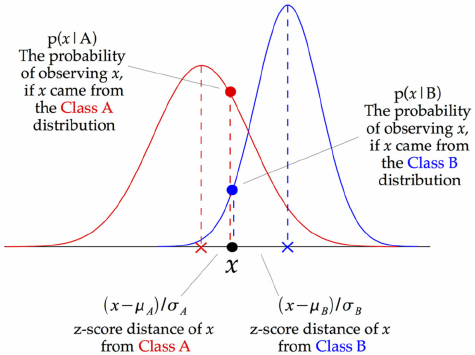
\includegraphics[width=8cm]{Figures/Background/GNB.png}
	\caption{Ejemplo de distribuciones en base a \textit{Gaussian Naive Bayes}}
	\label{GNB_BACKGROUND}
\end{figure}


\subsubsection*{Multi Layer Perceptron (MLP)}

%\textcolor{purple}{\textbf{Jose:} faltaría poner un par de referencias modernas.}

%\textbf{Luis: si explico el MLP en detalle, entraría en conflicto con la siguiente sección de modelos CNN, tendria que explicar de nuevo el Bakpropagation, gradientes, etc..}

%\textcolor{orange}{\textbf{Luis: } Hecho}

El Perceptrón Multicapa o \textit{Multi-Layer Perceptron (MLP)} es una arquitectura de red neuronal artificial. Es una generalización del Perceptrón simple y surgió como consecuencia de las limitaciones de dicha arquitectura en lo referente al problema de la separabilidad no lineal. El MLP es un aproximador universal, en el sentido de que cualquier función continua en un espacio $R^n$ puede aproximarse con un Perceptrón multicapa, con al menos una capa oculta de neuronas. Esto, sitúa al MLP como un modelo matemático útil a la hora de aproximar o interpolar relaciones no lineales entre datos de entrada y salida.

La arquitectura de Perceptrón multicapa se caracteriza porque tiene sus neuronas agrupadas en capas de diferentes niveles: la capa de entrada, las capas ocultas y la capa de salida. Las neuronas de la capa de entrada se encargan únicamente de recibir las señales del exterior y propagarlas a todas las neuronas de la siguiente capa. La última capa proporciona la respuesta de la red para cada uno de los patrones de entrada.

Este tipo de arquitecturas son ampliamente utilizadas en problemas de aprendizaje supervisado, como clasificación y regresión, y ofrecen un gran rendimiento en contextos muy variables. Por ejemplo, en publicaciones recientes, este tipo de modelos ha sido aplicado a problemas como segmentación de imágenes médicas para la prevención de múltiples enfermedades \cite{valanarasu2022unext}, para la clasificación de nubes de puntos en tres dimensiones \cite{choe2022pointmixer} o como apoyo para la predicción del tiempo estimado de trayectos en taxi de la ciudad de Nueva York \cite{poongodi2022new}. Al pertenecer a la familia de las redes neuronales, estos modelos aprenden los pesos asignados a cada una de las conexiones entre neuronas de las capas para dar lugar a las fases comunes de optimización de redes neuronales que detallarán en la sección \ref{CNN_SECTION}. En la Figura \ref{MLP_BACKGROUND} se puede observar un ejemplo de la arquitectura \textit{MLP} \cite{PEDRO2017111}.

\begin{figure}[H]
	\centering
	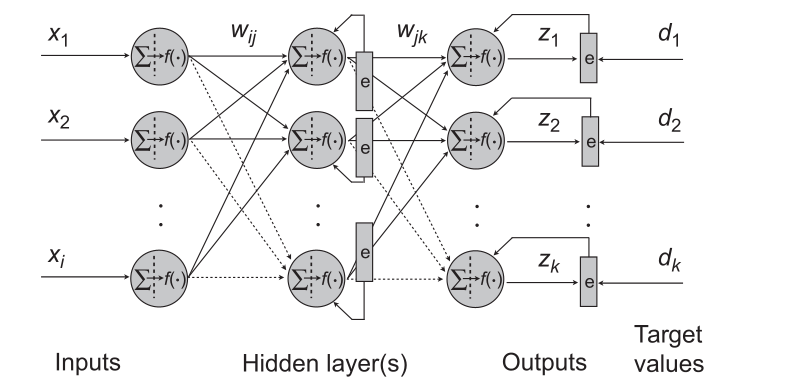
\includegraphics[width=10cm]{Figures/Background/MLP.png}
	\caption{Ejemplo de arquitectura \textit{MLP}}
	\label{MLP_BACKGROUND}
\end{figure}


% \begin{itemize}
	%     \item $x = (x_1, x_2, \ldots, x_n)$ as the input vector.
	%     \item $h^{(i)} = (h_1^{(i)}, h_2^{(i)}, \ldots, h_{m_i}^{(i)})$ as the activations of the $i$-th hidden layer.
	%     \item $W^{(i)}$ as the weight matrix connecting the $i$-th and $(i+1)$-th layers.
	%     \item $b^{(i)}$ as the bias vector added to the $i$-th layer.
	%     \item $f$ as the activation function.
	%     \item $y = (y_1, y_2, \ldots, y_k)$ as the output vector.
	% \end{itemize}

% The computation in an MLP can be represented as follows:

% \[
% h^{(i)} = f(W^{(i)}h^{(i-1)} + b^{(i)})
% \]

% where $h^{(i-1)}$ is the activation from the previous layer.

% The final output of the MLP is computed as:

% \[
% y = f(W^{(n)}h^{(n-1)} + b^{(n)})
% \]

% Here, $n$ represents the number of hidden layers in the MLP.


\subsubsection*{Regresión Logística (LR)}

%\textcolor{purple}{\textbf{Jose:} faltaría poner una imágen}

%\textcolor{orange}{\textbf{Luis: } Hecho}

La regresión logística es un modelo de aprendizaje estadístico utilizado históricamente para solventar problemas de clasificación binaria. Este método tiene como objetivo deducir la probabilidad de que ocurra un evento binario en función de uno o más predictores, siendo ampliamente extendido debido a su sencillez y capacidad de generalización. Por ejemplo, en investigaciones recientes, este modelo se ha aplicado de forma exitosa a la predicción de la pérdida de clientes en sectores de telecomunicación \cite{jain2020churn}, para la creación de rápidos protocolos computacionales de seguridad para preservar la privacidad del genoma humano \cite{de2021high}, o para la predicción de diabetes \cite{joshi2021predicting} en base a descriptores humanos. La regresión logística asigna un coeficiente a cada una de las variables predictoras, y estos son ajustados durante el proceso de aprendizaje para minimizar una función objetivo, normalmente R². Este proceso de ajuste de coeficientes en base a los datos de entrenamiento resulta en una combinación lineal de variables independientes ante nuevas muestras:

\[
z = \beta_0 + \beta_1 x_1 + \beta_2 x_2 + \dots + \beta_n x_n
\]
Donde $\beta_0, \beta_1, \dots, \beta_n$ son los coeficientes asignados a cada una de las variables predictoras, siendo $\beta_0$ el término de intercepción, y $z$ es el valor de la combinación de las características multiplicadas por dichos coeficientes.

La regresión logística hace uso de una función sigmoide, que transforma los valores continuos resultantes de la combinación lineal $z$ a una probabilidad de pertenencia a una clase en función de la separabilidad a través de esta dimensión de las muestras de entrenamiento.

\[
P(y = 1 | x) = \frac{1}{1 + e^{-z}}
\]

Donde $P(y = 1 | x)$ representa la probabilidad de la muestra x de pertenecer a la clase positiva. En la Figura \ref{LR_BACKGROUND} se puede observar un ejemplo de una clasificación mediante \textit{Regresión Logística} \cite{LR}.


\begin{figure}[h]
	\centering
	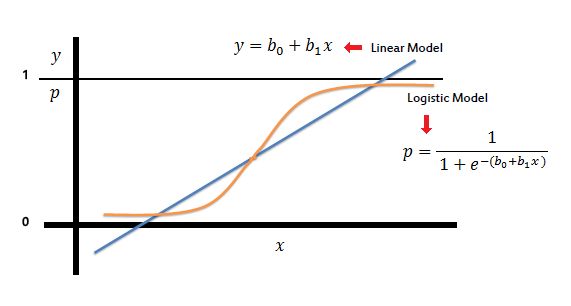
\includegraphics[width=10cm]{Figures/Background/LogReg_1.png}
	\caption{Ejemplo de clasificación mediante \textit{Regresión Logística}}
	\label{LR_BACKGROUND}
\end{figure}


\subsubsection*{k-Nearest Neighbours (KNN)}
%\textcolor{purple}{\textbf{Jose:} faltaría poner un par de referencias modernas y una imágen}
%\textcolor{orange}{\textbf{Luis: } Hecho}

El algoritmo \textit{k-Nearest Neighbours (KNN)} es un algoritmo de aprendizaje automático, ampliamente utilizado tanto para problemas de clasificación como de regresión. Estudios recientes han aplicado esta técnica para distintos propósitos, como agrupar datos de dimensiones arbitrarias para reconocer picos de densidad de forma eficiente \cite{chen2020fast}, como herramienta pra la clasificación de textos \cite{CHEN2020523}, o como apoyo para la detección de intrusos en redes inalámbricas \cite{liu2022enhanced} en base al número de usuarios por nodo, peticiones recibidas de la red, entre otras características. Este método se basa en la clasificación de nuevas muestras en base a la distancia de sus características respecto a la proyección de las muestras de entrenamiento sobre un espacio N-dimensional. Cuando una nueva muestra $x_0$ es clasificada, \textit{KNN} identifica los $K$ puntos más cercanos almacenados de sus muestras de entrenamiento respecto a las de la observación $x_0$ ($N_0$) y genera una probabilidad de pertenencia de la nueva muestra $x_0$ a la clase $j$, en función de la fracción de puntos de $N_0$ que pertenezcan a esa clase. La fórmula para calcular la probabilidad de pertenencia es la siguiente:

\[
P(y = j | X = x_0)  = \frac{1}{K} \sum_{i\in N_0} I(y_i = j)
\]

En la Figura \ref{KNN_BACKGROUND} se puede observar un ejemplo de clasificación mediante \textit{KNN} \cite{VIDUEIRAFERREIRA2015195}.

\begin{figure}[H]
	\centering
	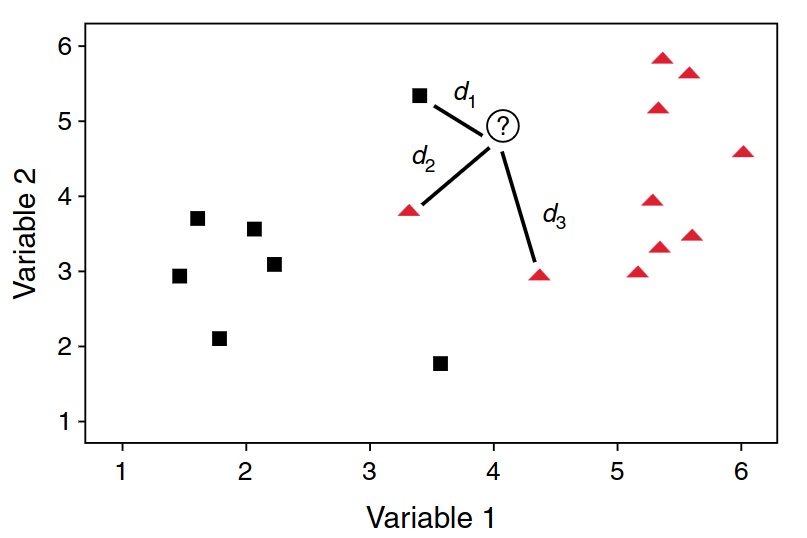
\includegraphics[width=10cm]{Figures/Background/KNN.png}
	\caption[Ejemplo de clasificación del \textit{KNN} ante una nueva muestra] {Ejemplo de clasificación del \textit{KNN} ante una nueva muestra. Se miden las distancias entre los $N$ puntos más cercanos de una nueva muestra y se clasifica como aquella que más vecinos cercanos presente}
	\label{KNN_BACKGROUND}
\end{figure}


\subsubsection*{Random Forest (RF)}
\label{RF_INTRODUCTION_TO_ENSEMBLES}

%\textcolor{purple}{\textbf{Jose:} faltaría poner un par de referencias modernas y una imágen}
%\textcolor{orange}{\textbf{Luis: } Hecho}


Los algoritmos \textit{Random Forest} son algoritmos basados en árboles de decisión que pertenecen al conjunto de modelos Ensembles. Los métodos \textit{Ensemble} son arquitecturas que están conformadas por varios modelos entrenados simultáneamente para dar lugar a un modelo predictivo final. Dentro de la categorización de Ensembles, el método \textit{Random Forest}, pertenece a la subcategoría \textit{Bagging}, cuya principal característica es que se apoyan en crear múltiples modelos que son entrenados con distintas técnicas de reemplazo (\textit{Bootstrap}) sobre los datos, conformando un modelo predictivo final como la combinación de la salida de cada uno de ellos de manera independiente por votación. Este tipo de modelos ha sido aplicado de forma efectiva en contextos muy variados, como para predicción de la contaminación de nitratos de aguas subterráneas \cite{HE2022133388}, predicción de precios de inmuebles en base a sus características \cite{ADETUNJI2022806} o para la medición de características geográficas socio-económicas importantes que influyeron en los fallecidos por \textit{COVID-19} en Estados Unidos \cite{GREKOUSIS2022102744}. Concretamente, \textit{Random Forest} se compone en $N$ árboles de decisión, donde cada uno de ellos es entrenado con un subconjunto de muestras y características de forma independiente al resto para dar lugar a un modelo combinado donde la predicción de nuevas muestras se elige aquella clase más votada de entre todo el conjunto de árboles. De forma generalizada, los modelos tipo \textit{Ensemble} son métodos robustos que son menos sensibles al sobreajuste de los datos gracias a sus técnicas de reemplazo durante su etapa de entrenamiento y la composición de un modelo final en base a varios modelos. En la Figura \ref{RF_BACKGROUND} se puede observar un ejemplo de la arquitectura \textit{Random Forest} \cite{MISRA2020243}.


\begin{figure}[H]
	\centering
	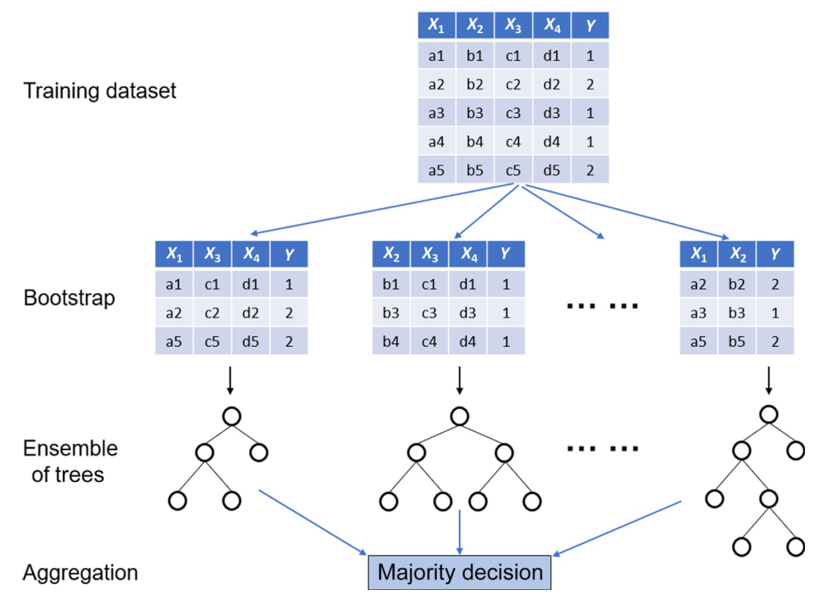
\includegraphics[width=10cm]{Figures/Background/RF.png}
	\caption[Ejemplo de arquitectura \textit{Ensemble Random Forest}]{Ejemplo de arquitectura \textit{Ensemble Random Forest}. El dataset es dividido en subconjuntos mediante \textit{Bootsrap} y se entrena un árbol de decisión sobre cada uno de ellos. La clasificación final viene dada por la predicción mayoritaria de los modelos}
	\label{RF_BACKGROUND}
\end{figure}

\subsubsection*{Support Vector Classifier (SVC)}

%\textcolor{purple}{\textbf{Jose:} faltaría poner un par de referencias modernas y una imágen}
%\textcolor{orange}{\textbf{Luis: } Hecho}

El \textit{Support Vector Classifier (SVC)} es un algoritmo de aprendizaje supervisado utilizado comúnmente para problemas de clasificación. Recientemente, este modelo ha sido aplicado a distintos contextos, como para la predicción de la deformación de los túneles durante su excavación en base a las condiciones geológicas \cite{zhou2022predicting}, como apoyo para la detección temprana de cánceres de piel \cite{arora2022bag} o incluso para la predicción de defectos en aplicaciones \textit{software} mediante métricas comunes en el desarrollo de los proyectos \cite{goyal2022effective}. Se basa en el concepto de encontrar un hiperplano óptimo que maximice la separabilidad de las clases de entrenamiento en base al espacio generado por la proyección de las características de los datos. El \textit{SVC} define estos hiperplanos en base a las muestras de distintas clases que más cerca se encuentren a lo largo del espacio N-dimensional. La fórmula que define un hiperplano para el \textit{SVC} en un problema de clasificación binario se define como:

\[
W \cdot X - b = 0
\]

En tiempo de predicción, el \textit{SVC} utiliza los hiperplanos definidos para determinar si una nueva muestra $x_0$ pertenece a una clase u otra mediante la siguiente ecuación:

\[
f({x_0}) = \text{sign}({W} \cdot {x_0} - b)
\]

Donde $W$ es el vector de pesos asociado a cada característica, $X$ es el vector de características de la muestra y $b$ es el término de sesgo.

En la Figura \ref{SVC_BACKGROUND} se puede ver un ejemplo de clasificación mediante \textit{SVC} \cite{MISRA2020243}.

\begin{figure}[H]
	\centering
	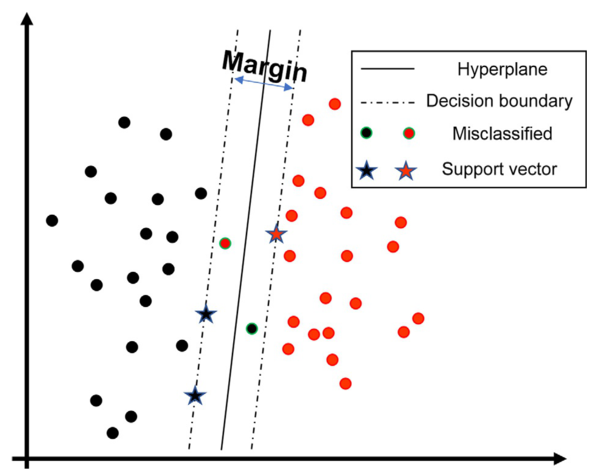
\includegraphics[width=7cm]{Figures/Background/SVC.png}
	\caption{Ejemplo de \textit{SVC}}
	\label{SVC_BACKGROUND}
\end{figure}

\section{Algoritmos CNN}
\label{CNN_SECTION}
%\underline{Explicación de diferentes algoritmos CNN con los que luego te comparas, con sus formulas y explicacion}

%\textcolor{blue}{\textbf{Luis: Yo creo que OK, hay que repasar el hilo que conecta los párrafos.}}\\


Las redes neuronales convolucionales \textit{(CNNs)} son modelos de inteligencia artificial supervisados que principalmente están orientados al reconocimiento de patrones en imágenes. Estos modelos han sido ampliamente utilizados para distintos objetivos dentro de este contexto, como clasificación de imágenes, detección de elementos de interés, o incluso han sido aplicadas a problemas de regresión. Tal es su rendimiento en estos problemas, que estas arquitecturas han sido extrapoladas al campo de la Inteligencia Artificial Generativa, ofreciendo soluciones en distintos problemas como la generación de imágenes artificiales a través de redes generativas adversarias (\textit{GANs}), segmentación de elementos de interés dentro de imágenes, o incluso en la representación de imágenes mediante vectores n-dimensionales para comparar la similitud de imágenes entre sí mediante redes siamesas.

La principal característica que distingue a estos modelos respecto al resto de redes neuronales y que las hace tan efectivas en problemas orientados a imágenes, es que su diseño se basa en capas convolucionales. Estas capas están compuestas por filtros, que durante el proceso de entrenamiento aprenden operaciones que se aplican sobre los datos de entrada, permitiendo así generar y reconocer patrones que se encuentren presentes en ellos.

Dentro de las redes neuronales convolucionales existen diferentes tipos, cada uno con sus ventajas y desventajas en función del problema que se quiera resolver. No obstante, existen partes comunes a ellas que es necesario mencionar, las capas de las que normalmente constan estas redes son las siguientes:

\begin{enumerate}
	\item \textbf{Capas convolucionales:} Estas capas aplican convoluciones sobre las muestras de entrada. Las convoluciones no son más que multiplicaciones sobre posiciones de un vector que calculan la suma ponderada de todos los vecinos de la muestra de entrada para dar lugar a un único resultado en su salida, que será asignado a la salida de la capa convolucional en la misma posición sobre la que se ha aplicado la operación sobre la muestra de entrada. Los valores de ponderación (pesos) de esta suma son aprendidos por la red en su etapa de entrenamiento.
	
	\item \textbf{Filtros:} Los filtros son pequeñas matrices de las que están compuestas las capas convolucionales y son utilizadas para realizar las operaciones. Cada uno de estos filtros tiene asociado una serie de pesos en cada posición de la matriz. Estos filtros, al ser aplicados, generan los denominados \textit{feature maps}, que no son más que mapas de activación sobre los que se aplicarán la función de activación.
	
	\item \textbf{Función de activación:} las funciones de activación de las \textit{CNN} introducen no linealidades, lo que permite a la red aprender patrones y relaciones complejas dentro de los datos. Normalmente, se aplica una función de activación como \textit{ReLU (Rectified Linear Unit)} a los mapas de características para introducir la no linealidad.
	
	\begin{center}
		$\text{ReLU}(x) = \max(0, x)$
	\end{center}
	
	\item \textbf{Capas Pooling:} estas capas aplican operaciones sobre los mapas de características con el objetivo de simplificar la información y reducir la dimensionalidad, que permite reducir la complejidad computacional de las redes durante su entrenamiento. Estas operaciones tienen una naturaleza de agrupación que son aplicadas en pequeñas zonas de los mapas de características para simplificar áreas y contemplar patrones relevantes en ellas. Estas operaciones pueden ser promediar un conjunto de características, mantener el mínimo de ellas o el máximo entre otras.
	
	\item \textbf{Capas Densas:} Las capas densas son capas que interconectan completamente un conjunto de entrada de neuronas con las neuronas especificadas en esta capa. A diferencia de su aplicación en otro tipo de redes neuronales, en las redes convolucionales estas capas toman como entrada el conjunto de características extraídas de los procesos convolucionales para dar lugar a una clasificación final.
	\begin{center}
		$z_i = \sum_{j=1}^{n} w_{ij} \cdot x_j + b_i$\\
		$y_i = f(z_i)$
	\end{center}
\end{enumerate}

%\subsubsection*{Proceso de entrenamiento de una red convolucional}

El proceso de aprendizaje de las redes neuronales está dividido en varias fases. Las redes en su etapa de entrenamiento realizan predicciones sobre los datos de entrada, aplicando operaciones matemáticas sobre ellos utilizando los pesos en cada etapa de la red, a esta etapa se le conoce como \textit{Forward Propagation}, y es definida mediante la siguiente fórmula:


\[
\mathbf{z}^{[l]} = \mathbf{W}^{[l]} \cdot \mathbf{a}^{[l-1]} + \mathbf{b}^{[l]},
\]

donde:
\begin{itemize}
	\item \(\mathbf{z}^{[l]}\) es la activación antes de aplicar la función de activación en la capa \(l\).
	\item \(\mathbf{W}^{[l]}\) es la matriz de pesos.
	\item \(\mathbf{a}^{[l-1]}\) es la salida de la capa anterior.
	\item \(\mathbf{b}^{[l]}\) es el vector de sesgo.
\end{itemize}

Posteriormente, en la capa clasificadora, los valores predichos son comparados con el valor real de las muestras que han sido introducidas en esta etapa a la red, de tal forma que el error que han producido sobre estas muestras durante esta fase es medible y calculado mediante una función de pérdida. Para llevar a cabo este proceso, es necesario introducir el concepto de función de pérdida que medirá el error durante la fase de entrenamiento


%\textbf{Función de pérdida}

Las funciones de pérdida en las redes neuronales miden el error producido por la red al realizar predicciones sobre los datos en su etapa de entrenamiento. Estas funciones tienen como objetivo comparar la calidad de la predicciones de la red respecto a la clase verdadera a la que pertenecen. Un valor alto de esta función indica un error alto en las predicciones, mientras que un valor bajo representa una buena calidad de predicciones:

\[
\text{Pérdida} = \text{Cálculo de Pérdida} (\text{Verdadero}, \text{Predicho})
\]

La función de pérdida más común en problemas de clasificación binaria es la \textit{Binary Cross Entropy} cuya fórmula es:

$$\text{Binary Cross Entropy} = \frac{-1}{N} \sum_{i=1}^{N} (y_{i}*\log{p_{i}}+ (1 - y_{i})*\log{(1-p_{i}})).$$

Con $N$ representando el número de muestras totales en el conjunto de datos, $y_i$ la etiqueta verdadera de la clase (0 ó 1) de la muestra actual y $p_i$ la probabilidad de que la muestra actual pertenezca a la clase $1$.

Esta ecuación penaliza en tiempo de entrenamiento la clasificación errónea de las muestras. El término $$(y_{i}*\log p_{i})$$ penaliza la probabilidad $p_i$ de pertenencia de la muestra $y_i$ a la clase $0$, siempre y cuando el valor verdadero de la muestra sea la clase $1$. Por el contrario, el término 
$$y_{i}*\log{p_{i}}+ (1 - y_{i})*\log{(1-p_{i}})$$
penaliza la probabilidad $p_i$ de la muestra $y_i$ de pertenencia a la clase $1$ siempre y cuando el valor real sea la clase $0$. Así, valores de probabilidad altos de la predicción de la red a las clases incorrectas, generan una acumulación del error. El símbolo negativo de la ecuación describe la minimización de esta función de pérdida. Esta función se utilizará para actualizar los pesos de toda la red mediante \textit{Back Propagation} de cara a minimizar esta función para la siguiente época. Una vez se define la función de pérdida de la red, la actualización de los pesos internos de las capas de la red y por tanto, el conocimiento de la misma sobre los datos, viene dado por el proceso de \textit{Back Propagation}.

% \textbf{Backward Pass (Calculating Gradients):}
% \[ \frac{\partial \text{Loss}}{\partial Z} = \frac{\partial \text{Loss}}{\partial A} \times \frac{\partial A}{\partial Z} \]
% \[ \frac{\partial \text{Loss}}{\partial W} = \frac{\partial \text{Loss}}{\partial Z} \cdot X^T \]
% \[ \frac{\partial \text{Loss}}{\partial b} = \text{sum of} \, \frac{\partial \text{Loss}}{\partial Z} \, \text{over the examples} \]

% \textbf{Updating Weights and Biases:}
% \[ W = W - \alpha \cdot \frac{\partial \text{Loss}}{\partial W} \]
% \[ b = b - \alpha \cdot \frac{\partial \text{Loss}}{\partial b} \]


%\textbf{Backpropagation}

La actualización de los pesos de la red, viene dada por el proceso de \textit{Back Propagation}. Este método utiliza la función de pérdida de la época actual para calcular la dirección en la que actualizar la red mediante el descenso por gradiente. Para actualizar los pesos de la red se hace uso de la regla de la cadena para actualizar los pesos de la red, esto permite calcular las derivadas parciales de la función de pérdida con respecto a los pesos de la red neuronal. Esto se aplica mediante el cálculo de las derivadas parciales de las capas superiores para calcular las derivadas de las capas inferiores. Comienza a partir de la capa de salida, retrocediendo a través de las capas ocultas, actualizando los pesos de la red conjuntamente en cada etapa. La siguiente fórmula representa la la actualización de los pesos para una de estas capas:


Gracias a la derivabilidad de las funciones que componen la red, en función de este error los pesos asociados a cada una de las capas de la red son optimizados con el objetivo de minimizar el error en la siguiente etapa de entrenamiento (\textit{Back Propagation}). Gracias a la repetición de estos procesos la red toma conocimiento sobre los datos:

\[
\mathbf{W}^{[l]} = \mathbf{W}^{[l]} - \alpha \frac{\partial J}{\partial \mathbf{W}^{[l]}},
\]

con:
\begin{itemize}
	\item \(\alpha\) es la tasa de aprendizaje.
	\item \(\frac{\partial J}{\partial \mathbf{W}^{[l]}}\) es el gradiente de la función de pérdida \(J\) con respecto a los pesos.
\end{itemize}

En este trabajo, se estudiarán en detalle dos tipos de redes de este tipo, las redes neuronales convolucionales unidimensionales, CNN-1D, y las redes neuronales convolucionales bidimensionales, CNN-2D).

\textbf{CNN-1D}

Las redes neuronales convolucionales unidimensionales son redes cuya característica principal es que los filtros que aplican en cada una de sus convoluciones son de una dimensión \cite{CNN1D}. Estos modelos son ampliamente utilizados para problemas orientados a detecciones de patrones en señales, donde la naturaleza de los datos es principalmente secuencial. Por ejemplo, algunas de las aplicaciones donde las \textit{CNN-1D} han demostrado ser efectivas han sido la monitorización de electrocardiograma en tiempo real \cite{Kiranyaz2017tt}, detección de daños estructurales basada en vibraciones en infraestructuras civiles \cite{khodabandehlou2019vibration} o para clasificación de audios musicales \cite{allamy20211d}. Estas arquitecturas son una buena opción en problemas de este tipo, tanto en la calidad de resultados que presentan en este dominio, como en la rapidez de inferencia que demuestran, permitiendo ser aplicadas en tiempo real en dispositivos que requieren baja demanda de recursos computacionales, como teléfonos móviles. Sin embargo, la principal limitación de estas arquitecturas se debe a que no terminan de adaptarse correctamente a encontrar patrones bidimensionales, debido a su naturaleza.
% $$(f * g)[n] = \sum_{m=0}^{M-1} f[m] \cdot g[n-m]$$

\textbf{CNN-2D}

Las redes neuronales convolucionales bidimensionales \textit{(CNN-2D)} son redes ampliamente utilizadas en todo tipo de problemas relativos a imágenes \cite{9451544}. La principal característica que distingue a estas redes es que están especialmente adaptadas a la naturaleza bidimensional de las imágenes, utilizando filtros de dos dimensiones para capturar los patrones presentes en estas. Muy distintos han sido los casos de estudio en los que se han aplicado estas arquitecturas, como clasificación de imágenes médicas para detección de enfermedades tempranas \cite{7064414}, IA generativa para re-identificación facial \cite{6909616} mediante generación de representaciones en los patrones detectados o la segmentación de objetos de interés en imágenes \cite{long2015fully}.

\section{Algoritmos de construcción de matrices}
\label{SOAT_MATRIX_ALGORITHM_CONSTRUCTION}

La tendencia de utilizar modelos neuronales convolucionales en los últimos años ha tenido un considerable incremento debido a la eficiencia y rendimiento que estos demuestran a lo largo de múltiples contextos. La particularidad de estos modelos es que trabajan sobre datos matriciales sobre las que pueden aplicar convoluciones para aprender patrones más o menos complejos. Gran parte de la naturaleza de los problemas que debe resolver el campo de la Inteligencia Artificial, tiene un origen tabular, es decir, los datos que se ofrecen están conformados por registros (bases de datos, hojas de cálculo, etc.). Al no disponer de una tipología matricial o en forma de imagen, este problema impide aplicar modelos convolucionales a este tipo de datos. Para sortear este problema, a lo largo de los últimos años se han ido desarrollando técnicas para transformar datos tabulares a matriciales con el fin de poder aplicar este tipo de modelos. La forma en la que se transforman datos tabulares a datos matriciales no tiene una solución trivial, ya que la composición resultante debe generar una estructura que tenga sentido para los modelos convolucionales, maximizando la forma de representar la información para estos modelos. 

En los últimos años se han diseñado distintas estrategias para ajustarse a este requisito, como la propuesta de \textit{OmicsMapNet} \cite{ma2019omicsmapnet}, un algoritmo orientado a construir representaciones matriciales de las características de los genes en pacientes que presentan cáncer. Para ello se consideran las descripciones bibliográficas de los genes para posicionar en localizaciones cercanas en la matriz aquellos que mayor semejanza presentan a través de \textit{Tree Map}. Otro de los enfoques referentes en el estado del arte es \textit{DeepInsight} \cite{Sharma2019}, que utiliza vectores de características de los datos originales para proyectarlos en un espacio bidimensional aplicando la visualización estadística \textit{T-SNE} \cite{van2008visualizing}, donde aquellas características más cercanas bajo este espacio son seleccionadas para situarlas en posiciones cercanas de la matriz final construida. Más recientemente, se presentó \textit{REFINED (REpresentation of Features as Images with NEighborhood Dependencies)} \cite{Bazgir2020}, una técnica que busca proyectar las características originales de los datos en un espacio bidimensional utilizando un escalador multidimensional bayesiano, que permite mantener la distribución de las características en su espacio dimensional original, posteriormente se aplica un algoritmo de Escalada Simple (\textit{hill climbing}) que optimiza la asignación de las características a los píxeles finales de la imagen.

En lo que respecta a uno de los enfoques más recientes en el estado del arte, se presenta \textit{Image Generator for Tabular Data (IGTD)} \cite{Zhu2021}, una técnica que se aplica sobre descriptores de genes en pacientes que sufren cáncer. Esta técnica asigna las características más correlacionadas entre sí a posiciones cercanas dentro de la matriz, con el objetivo de aplicar una red neuronal convolucional que pueda operar sobre ella. Para lograr esto hace uso de técnicas de minimización de rankings entre pares de características y técnicas de minimización de rankings entre píxeles, donde en cada iteración se reasignan pares de características a la posición de aquellas otras que no han sido consideradas desde hace tiempo. De esta forma se logra una representación final de la matriz que resulta en agrupación de características similares cercanas.

\section{Métodos de Remuestreo}
\label{SOAT_RESAMPLING}

%\textcolor{blue}{\textbf{Luis: repasar la redacción del último párrafo.}}

En el campo de la Inteligencia Artificial el problema del desbalanceo de los datos ha sido ampliamente estudiado a lo largo de los años debido a los inconvenientes que generan para el entrenamiento de ciertos modelos predictivos y la frecuencia con la que los datos presentan este problema. Un conjunto de datos desbalanceado, respecto a una clase a predecir, se define como aquel que dispone proporcionalmente de muchas más muestras pertenecientes a una clase respecto a las demás. Los modelos predictivos de Inteligencia Artificial aprenden y actualizan su conocimiento en base a los datos, y gran parte de ellos se entrenan prediciendo sobre las muestras de entrenamiento en su etapa de aprendizaje para posteriormente actualizar su conocimiento en base a la clase real a la que pertenecían dichas muestras. Si el conjunto de datos sobre el que aprende un modelo de inteligencia artificial presenta una clase desproporcionalmente mayoritaria, este será penalizado en más ocasiones cuando se equivoque al predecir estas muestras como cualquier otra clase, por lo que el modelo tenderá a evitar ser penalizado prediciendo la gran mayoría de las muestras de entrenamiento como la clase mayoritaria, de tal forma que se obtiene un modelo sesgado producido por un conjunto de datos desbalanceado.

En problemas de inteligencia artificial y aprendizaje estadístico es común aplicar técnicas que permitan igualar el número de muestras en conjuntos de datos donde se presenta desbalanceo, y para ello existen dos principales corrientes que tienen como objetivo reducir la diferencia entre el número de clases de los datos:

\begin{enumerate}
	\item La primera de ellas consiste en igualar el número de muestras de la clase minoritaria hasta llegar a la mayoritaria (\textit{upsampling}) mediante técnicas de reemplazamiento de datos mediante \textit{Random Oversampling} \cite{abdi2015combat} o \textit{Bootstrap} \cite{zoubir2007bootstrap} entre otros.
	\item La segunda filosofía consiste en eliminar aleatoriamente registros de la clase mayoritaria hasta llegar al número de la minoritaria (\textit{undersampling}) \cite{mohammed2020machine}. De esta forma se consigue un dataset balanceado que no provoque un sesgo en el entrenamiento de la red a costa de perder información sobre la clase mayoritaria.
\end{enumerate}

Por otra parte, existe un enfoque orientado al remuestreo de datos de las clases minoritarias mediante la generación de datos sintéticos. Estas técnicas generan nuevos datos utilizando distintos métodos, como modelos estadísticos o algoritmos para imitar patrones de datos reales. El objetivo de esta corriente es crear datos que se asemejen a los datos reales, tanto en propiedades estadísticas como en relaciones entre variables. Una de las técnicas más conocidas de generación de datos sintéticos es \textit{Borderline SMOTE-II} \cite{han2005borderline}.

\textit{SMOTE-II} funciona como generador de datos sintéticos, para ello hace uso del espacio generado al proyectar las características de los datos. En base a esto es posible generar nuevas muestras de las clases minoritarias que se encuentren cercanas al espacio de características que divide dicha clase con el resto que conviven en el conjunto de datos. Para ello, se proyecta una nueva muestra de la clase minoritaria entre la línea que divide una muestra aleatoria respecto a uno de sus vecinos más cercanos. Esta técnica permite generar datos sintéticos en base al contexto que conforman las muestras de la clase minoritaria hasta llegar a la mayoritaria.

\section{Métodos de optimización de hiperparámetros}
\label{HYPERPARAMETERS_OPTIMIZATION_METHODS}

En el campo del aprendizaje automático, la optimización de los hiperparámetros o \textit{Hyperparameters Optimization (HPO)} cobra un papel fundamental en el desarrollo de modelos predictivos. Los hiperparámetros son configuraciones establecidas durante la etapa previa a iniciar el proceso de aprendizaje, por lo que afectan de forma significativa a la forma en que el modelo aprende sobre los datos, hace predicciones sobre nuevas muestras y, por ende, a su rendimiento.

Es por esto por lo que una buena configuración de hiperparámetros es de vital importancia, un modelo potencialmente aplicable a un problema puede llegar a quedar inservible por el simple hecho de no tener una configuración eficiente de estos. Estas configuraciones son dependientes del problema, los datos, y el modelo propuesto para resolverlo. Además, el espacio de búsqueda (o combinación) de las configuraciones pueden ser más o menos amplias dependiendo de la naturaleza de cada modelo de aprendizaje y de las posibilidades de parametrización que este ofrezca. Debido a esto, es necesario optimizar los hiperparámetros, y existen distintos métodos por los que hacerlo.

La principal limitación a la hora de encontrar una configuración de hiperparámetros consistente es el coste que puede suponer en términos de recursos computacionales. Para evaluar una de estas configuraciones se requiere de entrenar el modelo con dicha configuración y evaluar el rendimiento que ofrece sobre datos que nunca ha visto. De esta forma se puede tener una intuición de la calidad de esos hiperparámetros, por lo que es necesario aplicar técnicas que permitan maximizar la calidad de la configuración minimizando el coste que esto supone.

%\textcolor{purple}{\textbf{Jose:} mirar la primera referencia}
%\textcolor{orange}{\textbf{Luis:} Hecho}

A lo largo del tiempo, distintos han sido los enfoques desarrollados para \textit{HPO} de modelos predictivos, cada uno con sus fortalezas y debilidades dependiendo del contexto en el que se apliquen \cite{yu2020hyperparameter}. Una de las técnicas clásicas y referentes debido a su precisión es la técnica \textit{Grid Search}. Esta técnica permite probar y es idónea para modelos ligeros y con pocos datos de entrenamiento, ya que permite probar cada combinación posible. Otra de las técnicas ampliamente reconocidas para el problema \textit{HPO} y basada en el método \textit{Grid Search}, es el \textit{Random Search} \cite{bergstra2012random}. Esta técnica establece también una parrilla donde se especifican los posibles valores que pueden tomar los hiperparámetros para seleccionar combinaciones de estos de manera aleatoria. Esto permite probar un gran número de configuraciones sin tener que pasar por cada una de las individualmente, reduciendo considerablemente el coste computacional permitiendo explorar zonas del espacio de búsqueda muy distintas. Sin embargo, al ser una selección aleatoria, la tendencia de este método no es la de converger y optimizar los hiperparámetros en base a la mejor solución, por lo que es muy probable que una configuración óptima nunca llegue a darse debido a su aleatoriedad.\\
Por otra parte, existen métodos de \textit{HPO} que utilizan modelos probabilísticos para calcular el set óptimo de hiperparámetros, como es el Optimizador Bayesiano. Este modelo busca la relación entre los parámetros de entrada y los valores de salida creando un modelo Gausiano probabilístico, reduciendo así el número de evaluaciones necesaria para llegar a una solución óptima.

Otro enfoque interesante para lograr una buena configuración de hiperparámetros es el uso de algoritmos genéticos \cite{alibrahim2021hyperparameter}. La naturaleza de estos algoritmos permite aplicarlos de forma eficiente al problema \textit{HPO}, ya que son métodos óptimos para problemas de minimización, donde en función de unos parámetros de entrada, estos son capaces de maximizar la calidad de la soluciones minimizando el esfuerzo que implica llegar a ella a lo largo de las generaciones.


\section{Algoritmos de medición de importancia de características}
\label{SOAT_FEATURE_IMPORTANCE_METHODS}

En el campo de la Inteligencia Artificial la medición de la importancia de las características entre los conjuntos de datos toma un papel fundamental para el análisis y desarrollo de modelos. Estas técnicas permiten conocer el peso que tienen cada una de las variables respecto al resto de ellas para un conjunto de datos, ya sea por la relación que presentan entre sí (fácilmente deducible por el ser humano o no), o por la importancia que han tenido a la hora de construir un modelo predictivo. Comúnmente, valores más altos de importancia representan una mayor relevancia de una característica  en el papel que ha interpretado en el entrenamiento de un modelo predictivo, mientras que valores más bajos suelen representar poca relevancia durante su ajuste.

En el estado del arte, existen distintos métodos que tienen como propósito medir el peso de las características en conjuntos de datos tanto para problemas de regresión como de clasificación. Uno de los enfoques más clásicos dentro del aprendizaje estadístico, para problemas de naturaleza regresiva (predicción de variables continuas), es la técnica de Regresión Lineal. Este método mide la magnitud de las variables en base al valor y la dirección de los coeficientes respecto al resultado del aprendizaje del método predictivo. Tomando como referencia esta base, existen enfoques más complejos derivados de esta técnica, como son las \textit{Elastic Net Regression}. Estos modelos durante el proceso de aprendizaje del modelo de regresión lineal utilizan términos de penalización para reducir los coeficientes del predictor, con el objetivo de introducir un componente de regularización, que favorecerá la generalización del modelo al evitar que pocos predictores sean demasiado influyentes en las predicciones de nuevas muestras. Por otra parte, existen técnicas orientadas exclusivamente a problemas de clasificación que permiten medir la importancia de las características. Un método muy común en este campo es la Regresión Logística, que para calcular la importancia de las variables, se utilizan las probabilidades logarítmicas para un cambio de una unidad en la variable predictiva. Los valores absolutos más grandes indican una relación más fuerte entre el predictor y la variable objetivo \cite{Saarela2021}.

% Permutation Feature Importance (https://academic.oup.com/bioinformatics/article/26/10/1340/193348?login=false)
% Feature Selection with Importance: no he encontrado nada en 2 min.\\
% Linear Regression Feature Importance: https://machinelearningmastery.com/calculate-feature-importance-with-python/

Por otra parte, existen otras técnicas que se alejan del aprendizaje estadístico y son métodos ampliamente utilizados para calcular la importancia de las variables, como son los modelos basados en filosofías de tipo \textit{Ensemble}, ya introducidos en la sección \ref{RF_INTRODUCTION_TO_ENSEMBLES}.

Dentro la filosofía de los modelos \textit{Ensemble}, los algoritmos \textit{Random Forest} han sido históricamente utilizados para calcular la importancia de las características de su entrenamiento. Para este fin, este algoritmo calcula mediante el peso que ha tenido cada característica a la hora de construir los árboles, en función del número de muestras que dividen cada uno de los niveles en los distintos árboles construidos.

No obstante, existe otra técnica más con mayor potencial dentro de los \textit{Ensembles} que tiene como base el funcionamiento de los \textit{Random Forest}, el algoritmo tipo \textit{Boosting XGBoost} \cite{Chen_2016}. Los algoritmos tipo \textit{Boosting} se caracterizan por crear modelos secuencialmente donde cada nuevo modelo se enfoca en corregir los errores cometidos por los modelos anteriores. \textit{XGBoost} construye $N$ árboles de decisión secuenciales, donde cada uno de estos se corrige el error cometido por el árbol anterior, reduciendo así el sesgo que pudiera llegar a producirse por datos desbalanceados y mejorando la precisión del modelo final, además ofrece de términos de penalización para evitar una complejidad excesiva del modelo final. Estos algoritmos disponen de una serie de hiperparámetros que deben ser configurados para un buen rendimiento, como limitar la profundidad de los árboles que se generan, la tasa de aprendizaje, que define la contribución de cada árbol al modelo final, o el número de instancias mínimas que debe separar un nodo para poder ser creado. Estas configuraciones permiten reducir el sobreajuste de los modelos en posibles casos muy específicos encontrados en los datos de entrenamiento. \textit{XGBoost} ha sido ampliamente utilizado a lo largo de los últimos años debido a su gran potencial para problemas muy diversos, como para la predicción de empresas que entran en bancarrota en base a sus características \cite{BenJabeur2023}, para predecir los niveles de agua subterránea en base a descriptores meteorológicos y geográficos \cite{IBRAHEMAHMEDOSMAN20211545}, o incluso para predecir la fluctuación del valor del oro a lo largo del tiempo \cite{Jabeur2021}. En la figura \ref{XGBOOST_BACKGROUND} se puede observar un ejemplo del algoritmo \textit{XGBoost} \cite{XGBOOST_IMAGE}.

\begin{figure}[H]
	\centering
	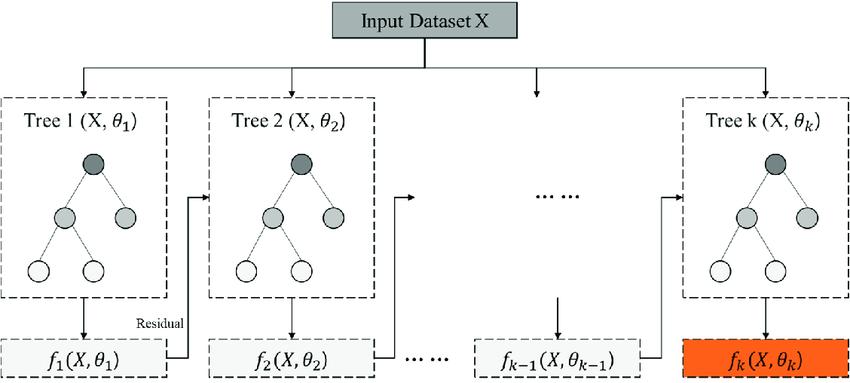
\includegraphics[width=10cm]{Figures/Background/XGBoost-model-process.png}
	\caption{Ejemplo de algoritmo \textit{XGBoost}}
	\label{XGBOOST_BACKGROUND}
\end{figure}


% \begin{figure}[H]
	%     \centering
	%     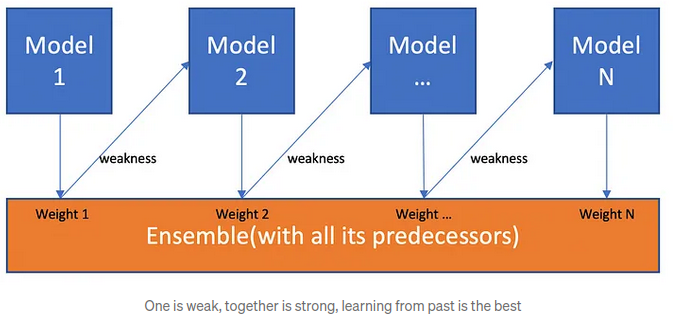
\includegraphics[width=14cm]{Figures/boosting_example.png}
	%     \caption{Alguna imagen así hecha por mi.}
	%     \label{BoostingExample}
	% \end{figure}

% [1] (https://towardsdatascience.com/boosting-algorithms-explained-d38f56ef3f30)

% [2] https://medium.com/geekculture/xgboost-versus-random-forest-898e42870f30


% https://towardsdatascience.com/best-practice-to-calculate-and-interpret-model-feature-importance-14f0e11ee660

% \section{Algoritmos Boosting}

% \textbf{Luis: jornada de reflexión sin redactar.} Yo creo que es que no hay boosting algorithms que ofrezcan la importancia de las características, creo  que de los pocos es el XGBoost. Hay que cercinoarse. No obstante, he visto esto:
% https://pubs.acs.org/doi/full/10.1021/ci0500379

\section{Algoritmos Genéticos}
% \underline{Explicación de los diferentes algoritmos genéticos que hay, formulas, descripcion, etc...}

% \textcolor{blue}{\textbf{Luis: Decir que son muy buenos para problemas de minimización (reducir coste y maximizar calidad, nos viene de lujo como entrada para la sección anterior)}}\\

Los algoritmos genéticos son métodos inspirados en la evolución biológica, que buscan optimizar soluciones a problemas matemáticos mediante la simulación de la evolución de una población de individuos que producen descendencia a lo largo de generaciones. Estos algoritmos han sido ampliamente utilizados en casos como la optimización del flujo de tráfico en la red para balancear la carga de los nodos \cite{5483775}, para analizar la capacidad de agua en el suelo mediante imágenes remotas \cite{PACHEPSKY1998213} o incluso para simular con el uso de autómatas distintas enfermedades como el \textit{COVID-19} \cite{GHOSH2020106692}. La principal fortaleza de estos algoritmos es que son métodos eficientes y seguros para llegar a soluciones aproximadas a la óptima ideal, reduciendo el coste computacional (en muchos casos exponencial), que supondría la búsqueda del óptimo global mediante métodos de combinación a lo largo de todo el espacio de búsqueda. Existen numerosos algoritmos genéticos conocidos, y muchos han sido aplicados a distintos contextos, tanto para problemas de objetivo único como a problemas multi-objetivo \cite{wang2020comparative}.

El funcionamiento de un algoritmo genético consta de una serie de etapas que son repetidas a lo largo de las sucesivas generaciones, concretamente \textit{inicialización, evaluación, selección, cruce, mutación y reemplazamiento}.

En la primera de ellas (\textit{inicialización}), se crea una población original de \textit{N} individuos aleatorios, donde cada uno de estos representa una posible solución al problema que se quiere optimizar (véase Figura \ref{GA_inicializacion}).

\begin{figure}[H]
	\centering
	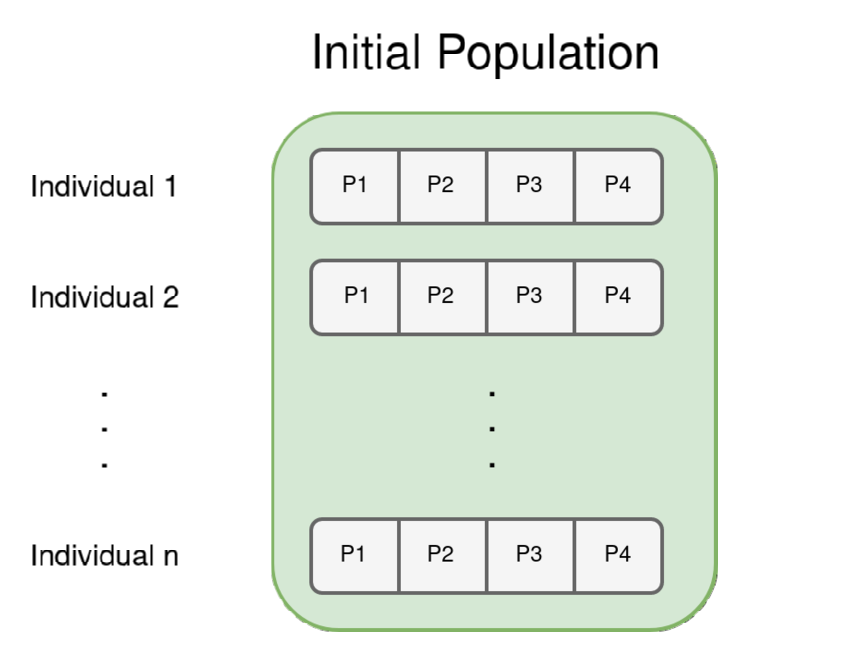
\includegraphics[width=6cm]{Figures/GA/inicializacion.png}
	\caption[Ejemplo de inicialización de individuos de algoritmo genético] {Ejemplo de inicialización de individuos de algoritmo genético. Este ejemplo consta de individuos compuestos por cuatro características}
	\label{GA_inicializacion}
\end{figure}


Estos individuos son evaluados mediante una función heurística, donde a cada uno se le asigna una puntuación de calidad en base a un criterio que mida el rendimiento que ofrece dicha solución al problema planteado (\textit{evaluación}), como se muestra en la Figura \ref{GA_selection}.


\begin{figure}[h]
	\centering
	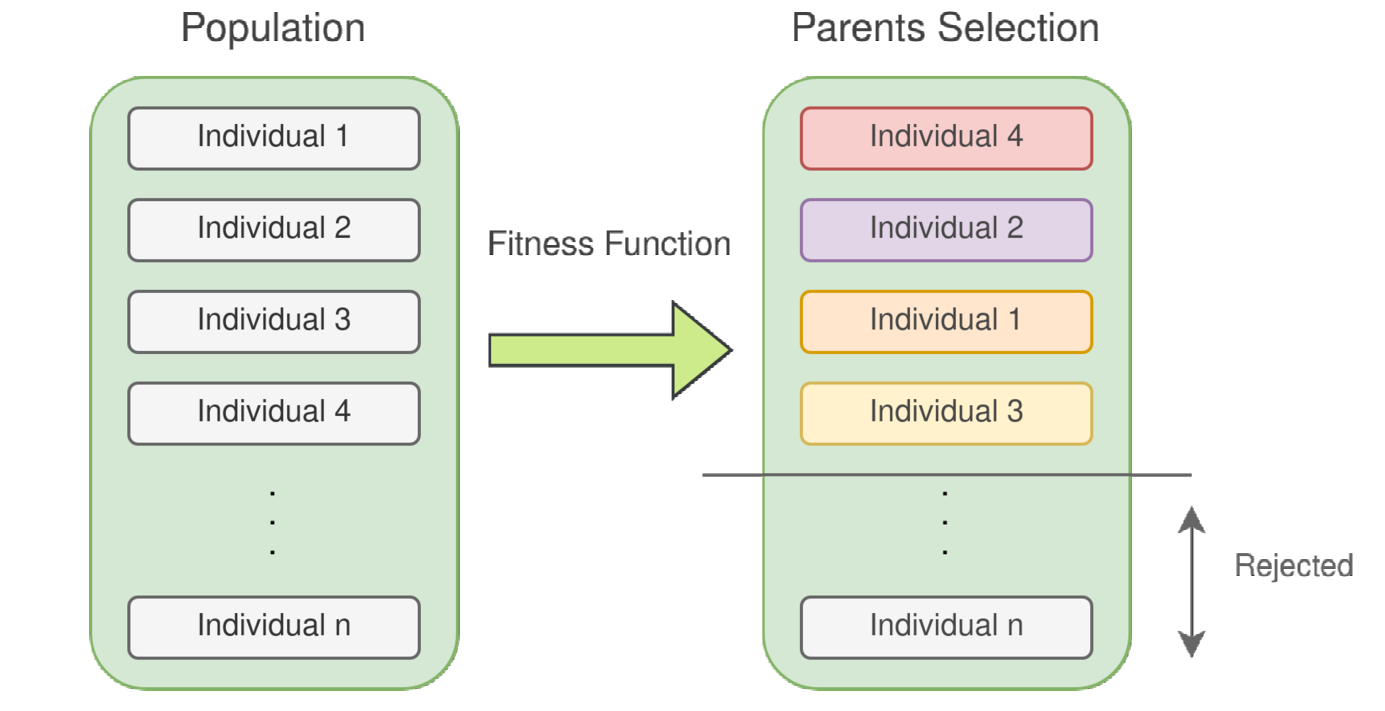
\includegraphics[width=8cm]{Figures/GA/selection.png}
	\caption[Ejemplo del proceso de selección de un algoritmo genético]{Ejemplo del proceso de selección de un algoritmo genético. En este ejemplo los cuatro mejores individuos de una generación son escogidos en base a su calidad en ofrecida por la función heurística (\textit{fitness function})}
	\label{GA_selection}
\end{figure}


Una vez se dispone de las puntuaciones de calidad, aquellos individuos que mejor se adapten al problema, es decir que mejor puntuación reciban, serán escogidos para dar lugar a descendencia (\textit{selección}). La información que contienen los \textit{M} mejores individuos es combinada entre sí (\textit{cruce}), simulando el intercambio de información producido en el intercambio genético en la naturaleza. Una vez se disponen de los nuevos individuos, estos pueden sufrir modificaciones aleatorias sobre su información resultante (\textit{mutación}), como se puede ver en la Figura \ref{GA_cruce_mutacion}.

\begin{figure}[h]
	\centering
	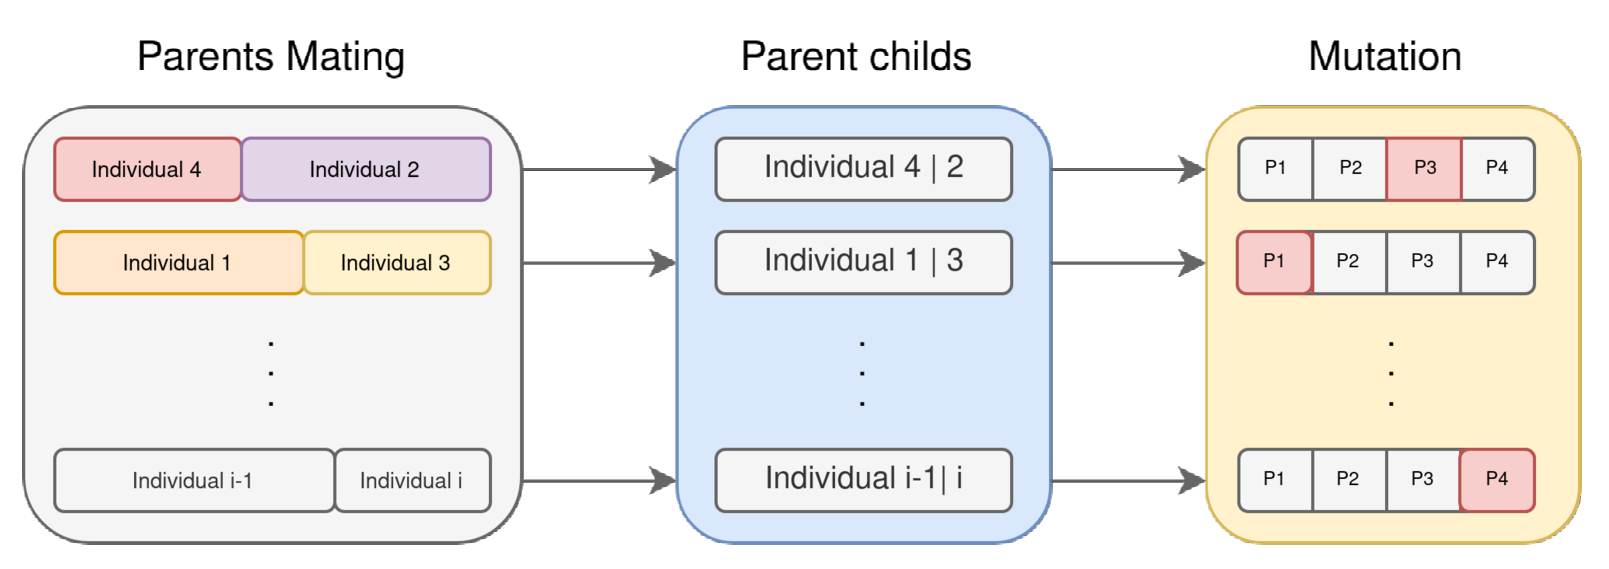
\includegraphics[width=10cm]{Figures/GA/cruce_mutacion.png}
	\caption[Ejemplo del proceso de cruce y mutación de un algoritmo genético] {Ejemplo del proceso de cruce y mutación de un algoritmo genético, donde se muta una característica de los individuos resultantes}
	\label{GA_cruce_mutacion}
\end{figure}

Como en cualquier población biológica, la combinación  de la misma información a lo largo de sucesivas generaciones provoca un estancamiento en la sociedad. La falta de diversidad en la población implica que no exista variabilidad en los individuos sucesores y por tanto que se tienda a explotar una zona del espacio de búsqueda provocando el riesgo de caer en un mínimo local del problema, es decir, una solución subóptima al problema respecto al mínimo global de la función buscado por estos algoritmos. Por este motivo es crucial introducir un componente aleatorio que pueda modificar la información de los individuos generados para tender a explorar este espacio de búsqueda. En este punto se evalúan los nuevos individuos y los \textit{M} miembros con peor puntuación de la población son eliminados, de esta forma la población en cada generación siempre constará de \textit{N} individuos. En caso de que existan individuos iguales en la población, estos son eliminados, lo que provoca que se integren en la población el mismo número de los que se han descartado. Estas etapas son repetidas a lo largo de varias generaciones hasta llegar a una condición de parada, tras la cual se seleccionará el individuo que mejor puntuación haya obtenido mediante la función heurística.

Cabe mencionar que dentro de la etapa de cruce, existen infinitas estrategias que se pueden aplicar para dar lugar al individuo descendiente. Por ejemplo, una de las más comunes suele consistir en dividir en dos a cada par de individuos que se reproducirán para generar su descendiente en base a composición de estas dos mitades. Otro método común, es seleccionar un punto aleatorio en cada proceso de descendencia del vector solución para dividir ambos progenitores, de tal forma que el individuo generado puede contener más información de un progenitor que de otro.


De esta forma, mediante la mejora continua de individuos a través de las generaciones, seleccionando los mejores y combinando su información entre sí, da lugar a una solución aproximada a la ideal a lo largo de las generaciones.

\section{Medidas de evaluación de una red neuronal}

En este apartado se presentan los indicadores de calidad utilizados para medir el rendimiento y generalización de los modelos expuestos en esta tesis. Uno de los componentes fundamentales en el desarrollo de modelos de inteligencia artificial es conocer la capacidad y calidad de los modelos ante la predicción de nuevas muestras que nunca ha visto durante su etapa de entrenamiento, tanto como para poder compararlos como para conocer en profundidad cómo se comportan los modelos ante nuevas situaciones.

Para evaluar los modelos, es común aplicar una fase de validación o de test, donde se utilizan los modelos para realizar predicciones contra muestras de las que se conoce su variable verdadera. De esta forma es posible comparar la calidad de los modelos respecto a muestras que nunca antes han visto y aplicar fórmulas y métricas que nos dan idea del rendimiento de los modelos. Para esto, es necesario introducir conceptos básicos que deben ser calculados para cada una de las clases que puede predecir el modelo.

\begin{enumerate}
	\item \textbf{True Positives (TP):} representan el número de muestras que han sido correctamente clasificadas por el modelo como positivas. Es decir, el modelo clasifica correctamente la muestra como la clase a la que pertenece.
	\item \textbf{True Negatives (TN):} representan el número de muestras que han sido correctamente clasificadas por el modelo como negativas. Es decir, el modelo
	\item \textbf{False Positives (FP):} representan el número de muestras que han sido incorrectamente clasificadas por el modelo como positivas. Es decir, el modelo ha clasificado una muestra que no pertenecía a esa clase como positiva.
	\item \textbf{False Negatives (FN):} representan el número de muestras que han sido incorrectamente clasificadas por el modelo como negativas. Es decir, el modelo ha clasificado una muestra positiva como negativa.
\end{enumerate}

En función del problema que nos encontremos, es posible que sea preferible un modelo que tienda a predecir con más facilidad futuras muestras a un tipo de clase respecto otra. Por ejemplo, es mejor predecir erróneamente que un accidente necesita asistencia (FP sobre la clase asistencia) y que luego no sea necesaria ninguna intervención, que predecir erróneamente uno que no necesita asistencia (FN sobre la clase No Asistencia). Este análisis del balance es posible evaluarlo gracias a los indicadores definidos anteriormente, no obstante, este tipo de decisiones son dependientes de la criticidad del problema que se quiere resolver.

Utilizando estos conceptos básicos es posible crear indicadores de calidad que ofrezcan más información para cada una de las clases predichas. En el estado del arte, se utilizan dos métricas comunes que pueden ser utilizadas para la composición de indicadores aún más complejos, estas métricas son calculadas para cada una de las posibles clases dentro del conjunto de datos.

La primera de ellas es la precisión (Precision), que mide el porcentaje de muestras clasificadas correctamente de una clase, respecto al total de muestras que existen de dicha clase en el conjunto de datos.

$$\text{Precision} = \frac{{\text{TP}}}{{\text{TP} + \text{FP}}}$$

Por otra parte, el recuerdo (\textit{Recall}) representa la proporción de elementos de una clase que el modelo identifica correctamente como esa clase.

$$\text{Recall} = \frac{{\text{TP}}}{{\text{TP} + \text{FN}}}$$

Existe otra métrica que combina los dos indicadores anteriores, considerando la precisión que tiene el modelo a la hora de predecir muestras como una clase y cuántos de los casos positivos fueron captados por el modelo (recuerdo), de tal forma que para cada cada una de las clases se pueda obtener una evaluación individual, siendo más sencillo en análisis sobre esto. 

$$\text{F1 score} = 2 \times \frac{{\text{precision} \times \text{recall}}}{{\text{precision} + \text{recall}}}$$


%\textcolor{red}{AQUI estaría interesante poner un minipárrafo destacando lo maravillosa que es esta medida, para que se suele usar, y tal. Más que nada porque luego la usamos para resaltar los buenos resultados obtenidos.}

%\textcolor{orange}{\textbf{Luis: } Hecho}

La métrica F1-Score es particularmente útil en problemas de clasificación binaria, sobre todo cuando existe un desbalanceo en las clases. Particularmente en estos casos, este indicador muestra información muy relevante en comparación a otras por sí solas, ya que toma en cuenta la combinación tanto de los falsos positivos como de los falsos negativos. Debido a la visión general del rendimiento de los modelos que ofrece en este tipo de casos, será la métrica definida para la evaluación de los modelos sen esta tesis.


 


\chapter{Construcción de un modelo general de predicción de la gravedad de un accidente de tráfico}

En este capítulo se describe la metodología para el desarrollo de un modelo general de predicción de gravedad de accidentes de tráfico aplicable a cualquier región e independiente a los datos que puedan estar disponibles en cada una de ellas. Para llegar a este fin, inicialmente se realizó una investigación y se implementó una primera metodología a modo de prototipo sobre la que aplicar modificaciones e hipótesis hasta llegar al objetivo final, un procedimiento que no fuese sensible a la disponibilidad de datos y fuera independiente de la región sobre la que se aplicase, es decir, un modelo general de predicción de la necesidad de asistencia en los accidentes de tráfico general. Por este motivo, este apartado se divide en dos subsecciones. La primera de ella describe la intuición sobre el primer prototipo, describiendo brevemente las fases que lo componen, los objetivos finales de este, incidiendo en las partes que han evolucionado respecto al modelo final. La siguiente sección de este apartado expone la metodología final tras la evolución del prototipo como referencia, justificando las decisiones tomadas en cada caso.

% \textcolor{blue}{\textbf{Luis: esta intro y todo el punto del modelo preeliminar no me termina de convencer, lo hablamos cuando podais.}}\\

\section{Modelo preliminar}
\label{METODOLOGIA_MODELO_PRELIMINAR}

%\sout{\textcolor{red}{MANU: En una primera fase de la tesis doctoral, se propuso un modelo preliminar aplicado a un dataset concreto, orientado a la gravedad del accidente, estableciendo una clasificación de 3 niveles (leve, severo y fatal). Con el objetivo principal de la tesis de realizar un modelo general y la reclasificación del problema a la necesidad de asistencia en un accidente de tráfico, se explica en este apartado brevemente el modelo preliminar, y explicado con total detalle en la siguiente sección 4.3 el modelo general que se propone.}}


En una primera fase de la investigación, se propuso un modelo preliminar de predicción de la gravedad de accidentes de tráfico aplicado a una ciudad \cite{PEREZSALA2023113245}, teniendo como meta la predicción de la gravedad de los accidentes en base a 3 niveles (leve, severo y fatal). Como el objetivo de este trabajo es diseñar un modelo predictivo general a cualquier ciudad, en este apartado se expondrá brevemente el enfoque del modelo preliminar,a modo de introducción y acentuando los matices que condujeron a la reclasificación posterior de las clases que describían la necesidad de asistencia. El modelo general que se propone se explicará con total detalle en la siguiente sección \ref{METODOLOGIA_GTAAF}.

Este primer prototipo se presentó en \cite{PEREZSALA2023113245} y se implementó con el objetivo de predecir la gravedad de los accidentes de tráfico utilizando un dataset de la ciudad de Madrid. Concretamente, se dividió la gravedad de los accidentes entres categorías distintas que estaban en ese conjunto de datos: (1) Leves, (2) Severos y (3) Fatales.

Para llegar al entrenamiento del modelo predictivo, se diseñó una metodología compuesta por cinco fases secuenciales, mostradas en la Figura \ref{figDegree}. Esta metodología tenía como objetivo realizar transformaciones y operaciones sobre datos, inicialmente tabulares, para transformarlos en datos matriciales sobre los que pudieran operar modelos diseñados para tratar imágenes. De esta forma era posible experimentar con dos modelos convolucionales, el primero de ellos unidimensional y el segundo bidimensional, CNN-1D y CNN-2D respectivamente.

Primeramente fue necesario definir una categorización de características, las cuales fueron utilizadas como apoyo para la construcción de estas matrices. Para la construcción de las matrices que alimentan las redes convolucionales se le asignó una importancia a cada variable dentro del conjunto de datos con la finalidad de situarlas en determinados lugares de estas matrices. Es decir, dependiendo de la importancia asignada a cada variable, se le asignaba una posición en la matriz. 

Finalmente la metodología y los modelos convolucionales propuestos se compararon con otros tres modelos del estado del arte \textit{(Naive Bayes, Support Vector Classifier y k-Nearest Neighbor)} para evaluar sus rendimientos respectivos en el dataset de la ciudad de Madrid.

A continuación se enumeran las etapas que definen el flujo de la metodología prototipo.

\begin{figure}[h]
	\centering
	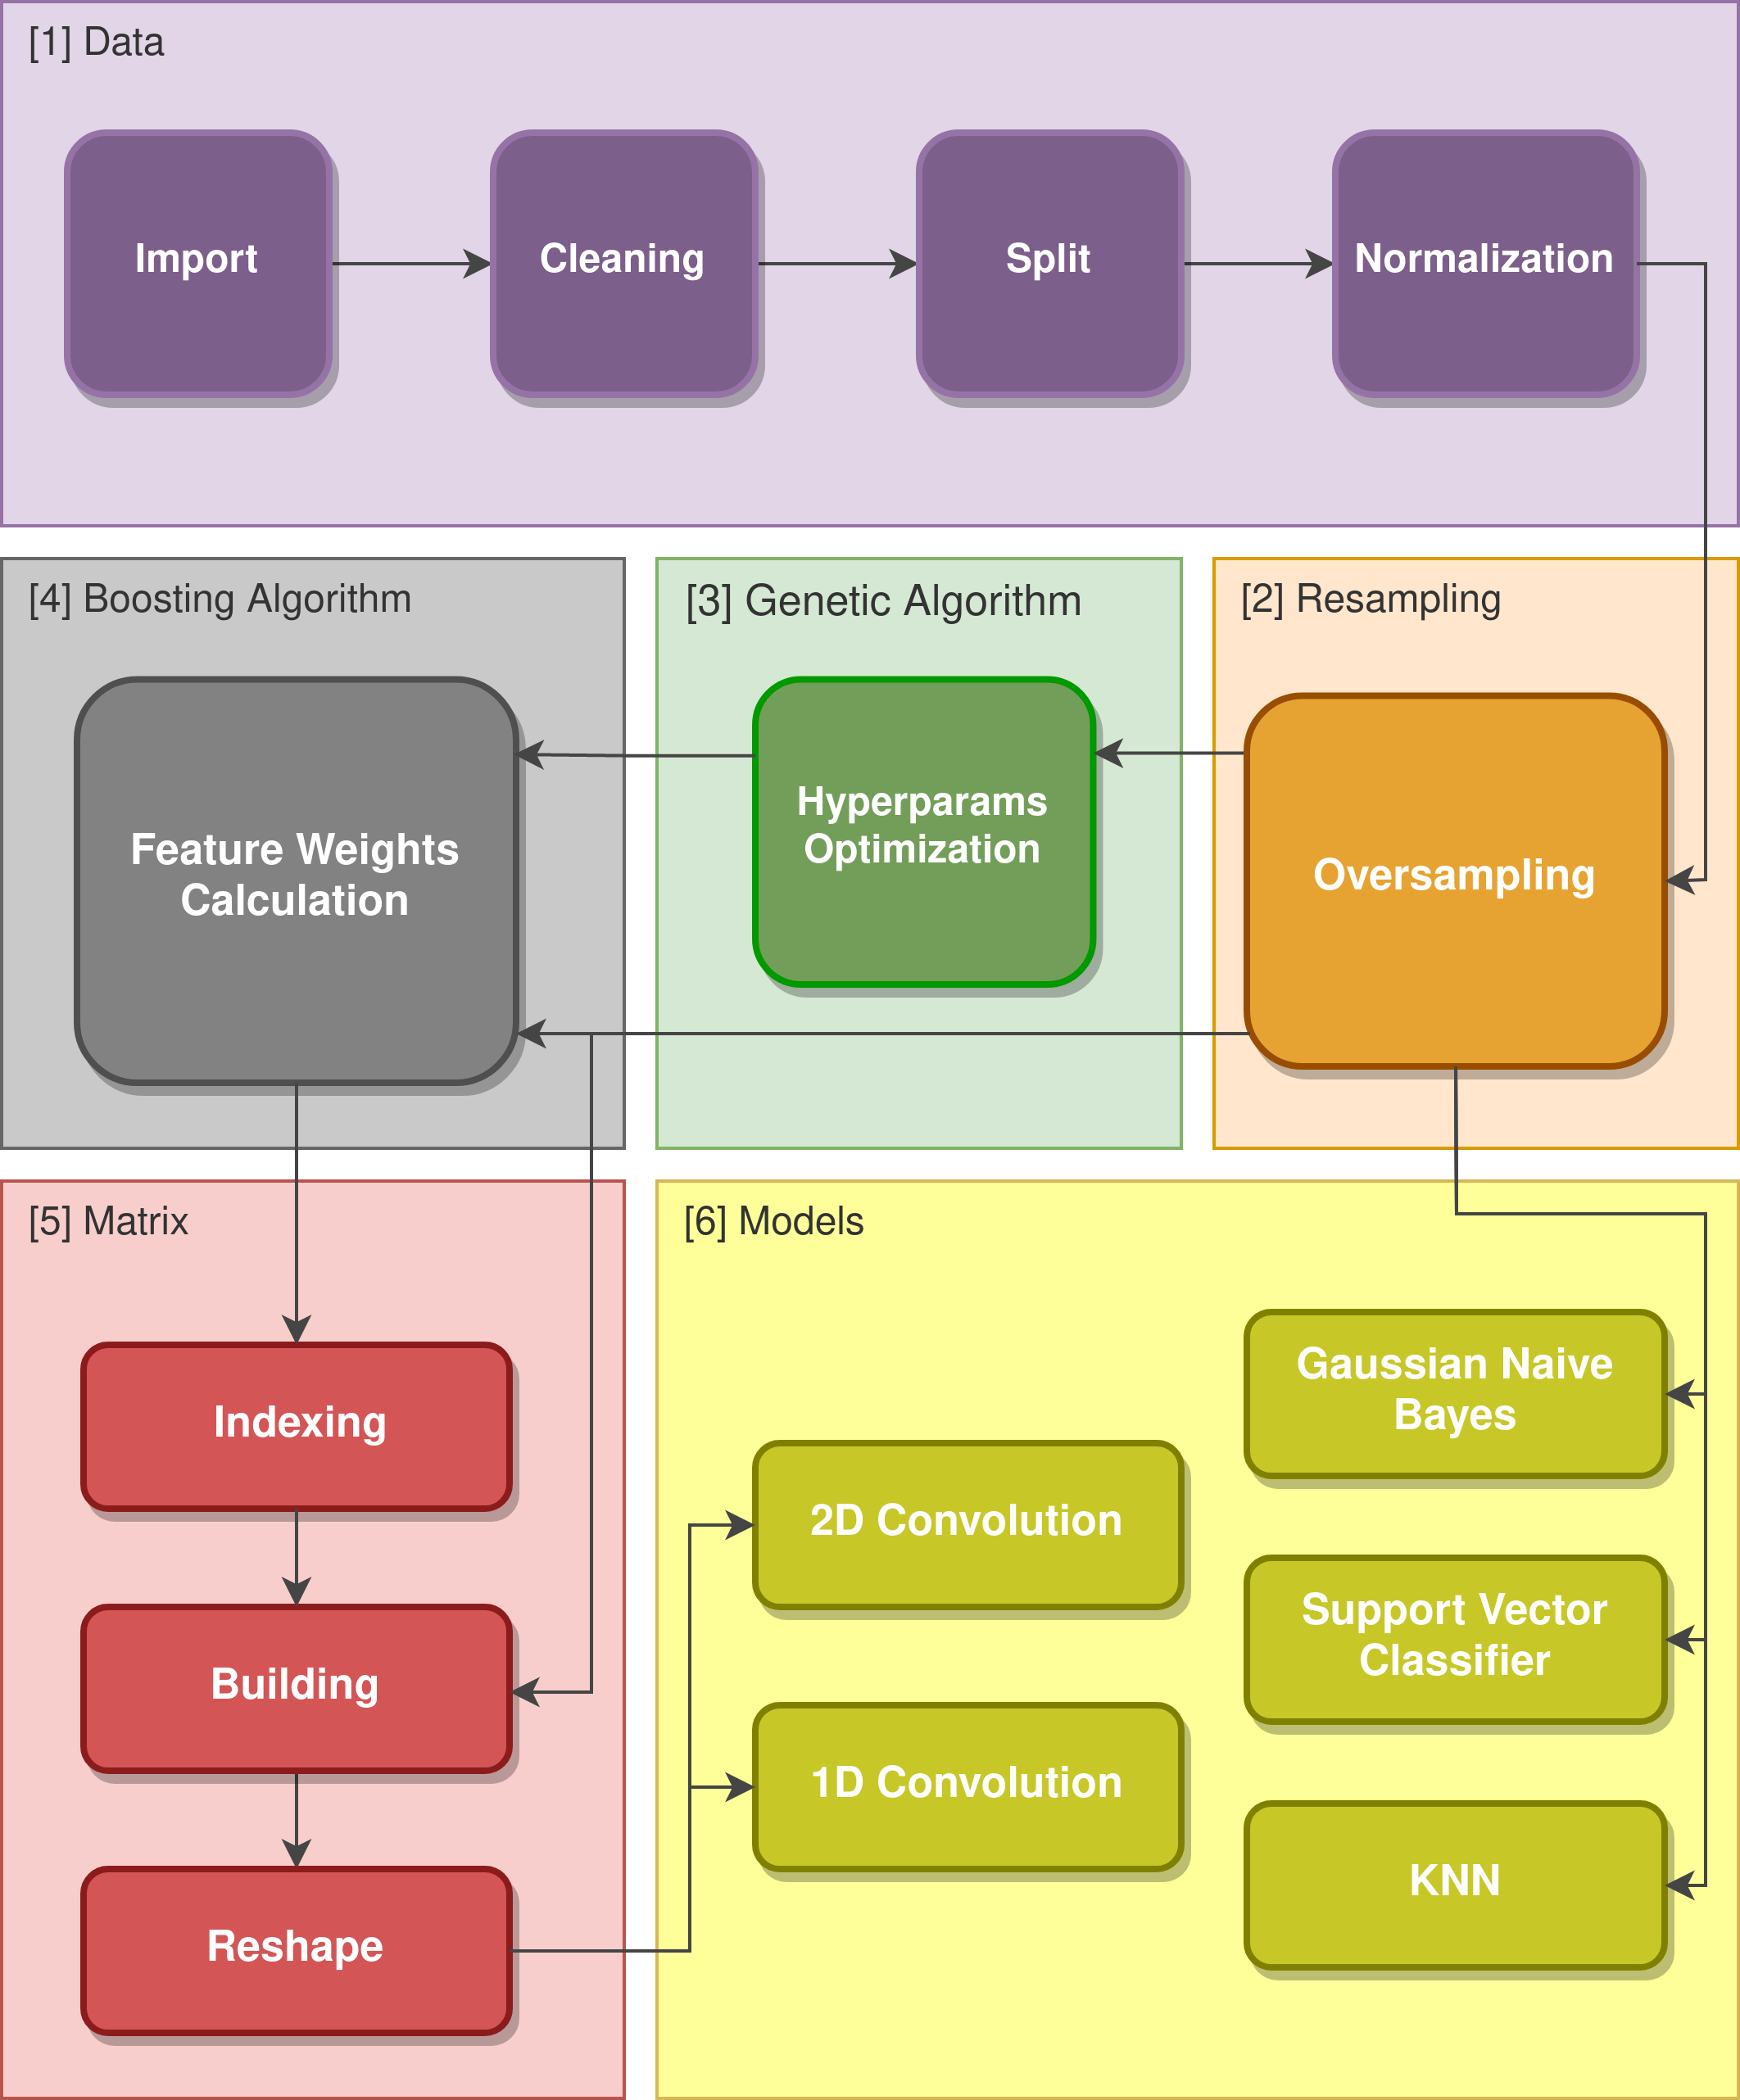
\includegraphics[width=3.5in]{Figures/1stPaper/Data_flow.png}
	\caption{Diagrama de flujo del modelo preliminar propuesto}
	\label{figDegree}
\end{figure}

La primera fase de esta metodología prototipo, (1) en la Figura \ref{figDegree}, está orientada al tratamiento de los datos. Los datos originales del dataset eran datos en bruto, donde se podían encontrar errores en los valores, valores atípicos y variables con valores cualitativos que había que discretizar. Es por esto que en esta etapa se diseñaron métodos para tratar estos datos, concretamente aplicándoles un proceso de limpieza, una discretización para que fuesen interpretables por los modelos, un tratamiento para su normalización y otro para evitar que estuviesen sobredimensionados.

En una segunda fase (2), se aplicó un proceso para trabajar sobre el desbalanceo de los datos presente el dataset ya que, debido a la naturaleza de los accidentes de tráfico, gran parte de ellos eran de tipo leve, mientras que el resto de accidentes (severos y fatales), presentaban una proporción mucho menor. Para evitar un sesgo en los modelos, es decir, una tendencia a predecir cualquier nueva muestra como accidente tipo leve (la de clase mayoritaria), se estudiaron distintas técnicas de balanceo de datos. Finalmente, se utilizó la técnica \textit{Borderline SMOTE-II} para balancear las clases minoritarias, aplicando generación de datos sintéticos para igualar el número de muestras de las otras dos clases hasta llegar a la mayoritaria.

Una tercera fase (3) buscaba transformar los datos tabulares resultantes a datos matriciales interpretables por los modelos convolucionales. Para esto se requería de algún tipo de estrategia para la asignación de cada una de las variables del dataset a coordenadas dentro de una matriz bidimensional con el objetivo de aplicar los modelos convolucionales propuestos en este prototipo. Para llevar a cabo esto, se tomó una estrategia que requería de conocer la importancia de cada variable dentro del conjunto de datos. Como método para hallar el peso de cada característica dentro del dataset se utilizó un algoritmo tipo \textit{Boosting}. Los algoritmos tipo \textit{Boosting} son clasificadores que ofrecen la importancia numérica de cada variable en función del peso que han tenido durante su entrenamiento. Estos algoritmos necesitan una configuración de hiperparámetros que se optimizaron mediante la evolución de las posibles configuraciones a través de un algoritmo genético (4).

Una vez se disponían de los pesos de las características gracias al cálculo del algoritmo tipo \textit{Boosting} (5), se categorizaron las variables en distintas categorías (6) para tener una referencia bidimensional sobre la que comenzar a asignar las variables. En primer lugar se calculó el peso total de las categorías, que era la suma de los pesos de cada una de las variables que contenía. Como resultado de esto, cada categoría se indexaba a una fila de la matriz, donde aquella que más peso presentaba era asignada a la fila central, la segunda en la posición inmediatamente superior, la siguiente en la inferior y así sucesivamente. Por otro lado, las características que las componían se asociaban a las columnas dentro de su categoría de forma similar, la de mayor peso en la posición central, la siguiente en su posición inmediatamente a la izquierda, la siguiente a la derecha, etc. Como resultado de este proceso, cada registro perteneciente al dataset original era transformado en una matriz de tamaño $5\times5$.

Las arquitecturas que se propusieron en la fase prototipo eran dos redes convolucionales, de una y dos dimensiones. Estas constaban de cuatro capas convolucionales con tamaños de \textit{kernels}, de $(1 \times 3)$ para la CNN-1D, y $(3 \times 3)$ para la CNN-2D respectivamente. Estos \textit{kernels} se proyectaban en $256$ y $512$ canales para formar el filtro convolucional asociado con cada capa. Posteriormente se aplicaba un proceso de normalización de batch a la salida de cada uno de los mapas de características. El \textit{padding} de los \textit{kernels} estableció en $1$ para ambos tipos de redes, de modo que las convoluciones se aplicaban agregando ceros a los límites de las matrices, de $1$ para la CNN-1D y ${1, 1}$ para la CNN-2D. Por lo tanto, el desplazamiento de los núcleos se realizaba elemento a elemento en ambas redes. En la salida de cada capa convolucional, se aplicaba la función de activación \textit{Rectified Linear Unit (ReLU)}. La salida de la última capa de convolución transformaba los mapas de características generados de tamaño $5 \times 5$ a un vector unidimensional de $1 \times 25$. A continuación, se aplicaba una capa densa que conectaba cada uno de los $25$ nodos de la capa aplanada con los $128$ nodos de la capa densa, que generaba los \textit{logits} antes de aplicar la última función de activación \textit{Softmax} que devolvía la clase predicha. En la figura \ref{TASPCNNIMAGE} se observa el diseño de la arquitectura de la red propuesta CNN-2D.

\begin{figure}[H]
	\centering
	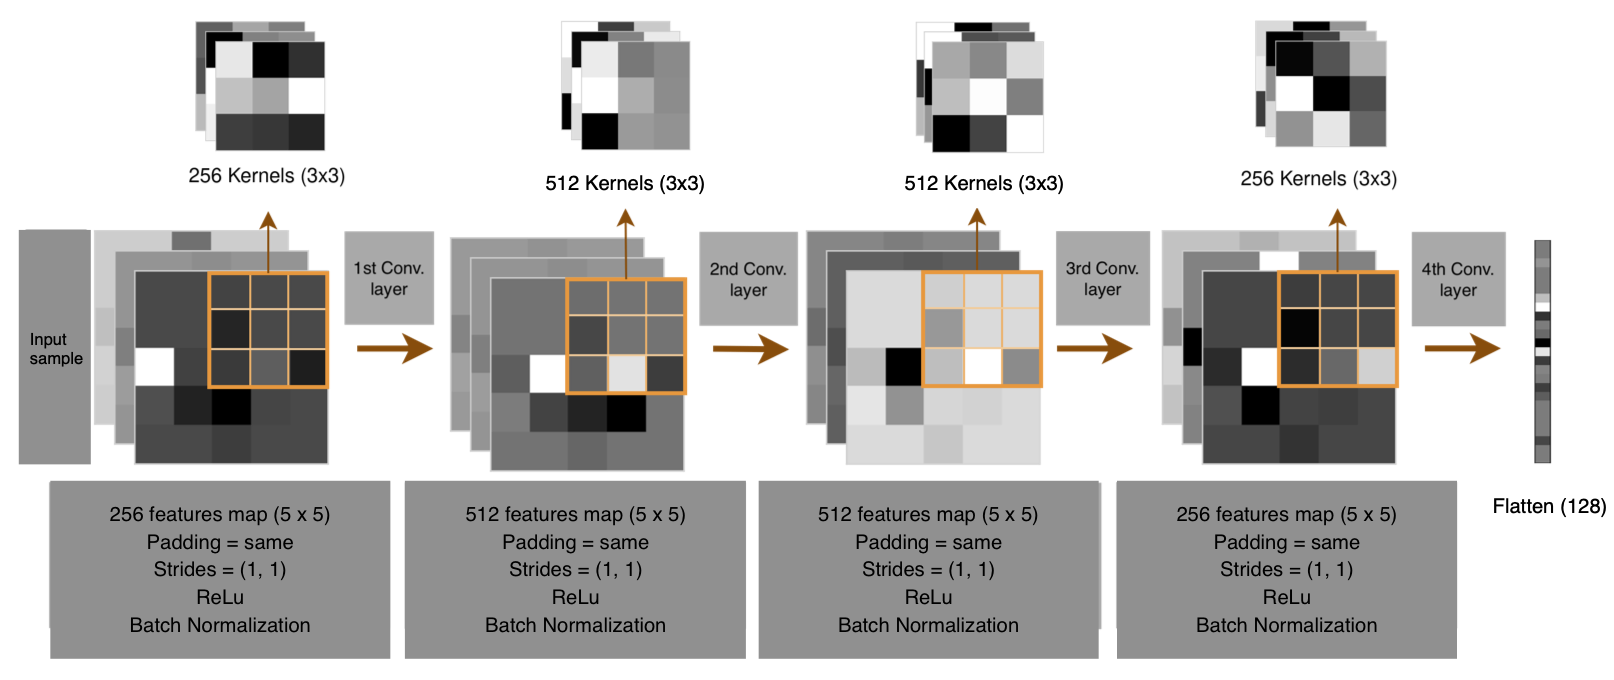
\includegraphics[width=15cm]{Figures/1stPaper/TASPCNN.png}
	\caption{Arquitectura de la red neuronal convolucional 2D}
	\label{TASPCNNIMAGE}
\end{figure}

En última instancia (6), los dos modelos propuestos, CNN-1D y CNN-2D se compararon contra tres modelos del estado del arte, utilizando como referencia de generalización el indicador \textit{F1-Score} sobre conjuntos de datos de test.


\subsubsection*{Aprendizaje resultante del prototipo}

% \underline{Aquí voy a poner las intuiciones de mejora, luego en GTAAF pongo las soluciones a estos problemas?}

Una vez aplicada la metodología sobre el conjunto de datos da Madrid, se analizaron los resultados que esta ofrecía sobre el conjunto de datos de test. Esto sirvió para observar ciertas debilidades y localizar puntos de mejora que podrían aumentar el rendimiento de cara a implementar una metodología generalizable a cualquier región.

En primer lugar, se observó que la decisión de dividir los accidentes de tráfico en tres clases (leves, severos y fatales) era un condicionante que perjudicaba considerablemente el rendimiento del modelo. Al tener dos clases notablemente desproporcionadas respecto a la mayoritaria, la generación de datos sintéticos podría carecer de sentido a nivel práctico. Esto hizo que se pensara en agrupar los accidentes en dos categorías (1: leves y 2: graves y fatales) con la finalidad de mejorar el rendimiento del modelo a nivel funcional al no disponer de clases intermedias además de capturar más información al sumar dos tipos de clases.

% El siguiente paso para resolver esto fue la categorización de estos accidentes en dos clases, además de implementar un proceso de filtrado de áreas que uscaba rebajar el número de accidentes tipo leve de forma natural en el conjunto de datos.

Al observarse incongruencias en la interpretación sobre los valores numéricos asignados a determinadas variables, se plantearon cuestiones sobre la discretización de los datos y su inclusión en áreas geolocalizadas. Además, observando las curvas de aprendizaje en las gráficas de entrenamiento de los modelos, se propuso la de mejora de añadir más características a la matriz de entrada a las redes convolucionales, planteándose la inclusión de más variables que pudiesen ser obtenidas en base a transformaciones sobre los datos existentes para aportar más información al modelo.

\section{Modelo GTAAF}
\label{METODOLOGIA_GTAAF}

% \textbf{Luis: aquí de alguna forma te tienes que traer la categorización de la sección de resultados, para decir que la metodología generalizable se usa en base a esto.}\\
%\textcolor{red}{Luis: este párrafo inical entra en colapso con la sección de Resultados 1.1.1 Descripción de datos, se dicen cosas muy parecidas. Hay que analizar cuál nos gusta más y reestructurarlo}
%\textcolor{purple}{\textbf{Jose:} No estra en colapso con nada, si se repite dos veces no pasa nada...}
%\textcolor{orange}{\textbf{Luis: } vale, gracias Jose.}

% \textcolor{orange}{\textbf{Luis: Me parece muy circular todo esto, todo el rato diciendo lo mismo. Opiniones?}}

Después de analizar los resultados ofrecidos del primer prototipo, se propusieron una serie de modificaciones en el modelo enfocadas a mejorar las debilidades observadas. Estos cambios se estructuraron en una nueva metodología denominada GTAAF (General Model for Traffic Accident Assistance Forecasting) que busca incrementar el rendimiento del prototipo y cuyo principal objetivo es diseñar e implementar un procedimiento de predicción de asistencia de accidentes de tráfico generalizable a cualquier dataset y región. 

El principal problema observado en los conjuntos de datos de accidentes de tráfico es que, dependiendo de la región y/o gobierno que los ofrezca, estos disponen de información diferente, debido principalmente al coste que supone obtener ciertos datos y a la naturaleza social de la población. Es por esto que, la implementación de un modelo de predicción de necesidad de asistencia en accidentes de tráfico general, requiere un trabajo de análisis de la categorización de las variables disponibles y cuáles pueden ser influyentes en la necesidad de asistencia.

Con la finalidad de solventar estos problemas y presentar una generalización del modelo que sea independiente de los datos disponibles, la metodología GTAAF propuesta se basa en categorización de las características disponibles individuales dependientes de cada conjunto de datos. Así, en función de la naturaleza a la que pertenezca cada dato disponible estos puedan ser asignados a una de las categorías propuestas en esta metodología, cuyas propiedades son de fácil adquisición. Esto sortea las peculiaridades individuales de la disponibilidad de datos de cualquier región. 

Para evaluar la eficacia del modelo GTAAF, se compara con otros seis modelos del estado del arte a lo largo de ocho regiones distintas en las mismas condiciones.

En esta sección se explicará con detalle, cada una de las etapas por las que pasan los datos, la justificación de las decisiones tomadas para la construcción de esta metodología y las principales diferencias entre la versión preliminar y la versión final.

En primera instancia, las fases de la nueva metodología son asignadas a tres etapas claramente diferenciadas: (en naranja en la Figura \ref{DataFlow}) la fase de Pre-procesamiento, donde se contemplan procesos de limpieza de datos, transformación y balanceo de datos, (en gris) la fase de Postprocesado donde se aplican técnicas de transformación para representar los datos de accidentes en formato tabular a formato matricial, y (en azul) la fase de entrenamiento, donde se entrenará un modelo neuronal convolucional en base a esta representación para predecir la necesidad de asistencia en los accidentes. En la figura \ref{DataFlow} se muestran, en modo de diagrama, cada una de las fases que componen la metodología GTAAF.

\begin{figure}[H]
	\centering
	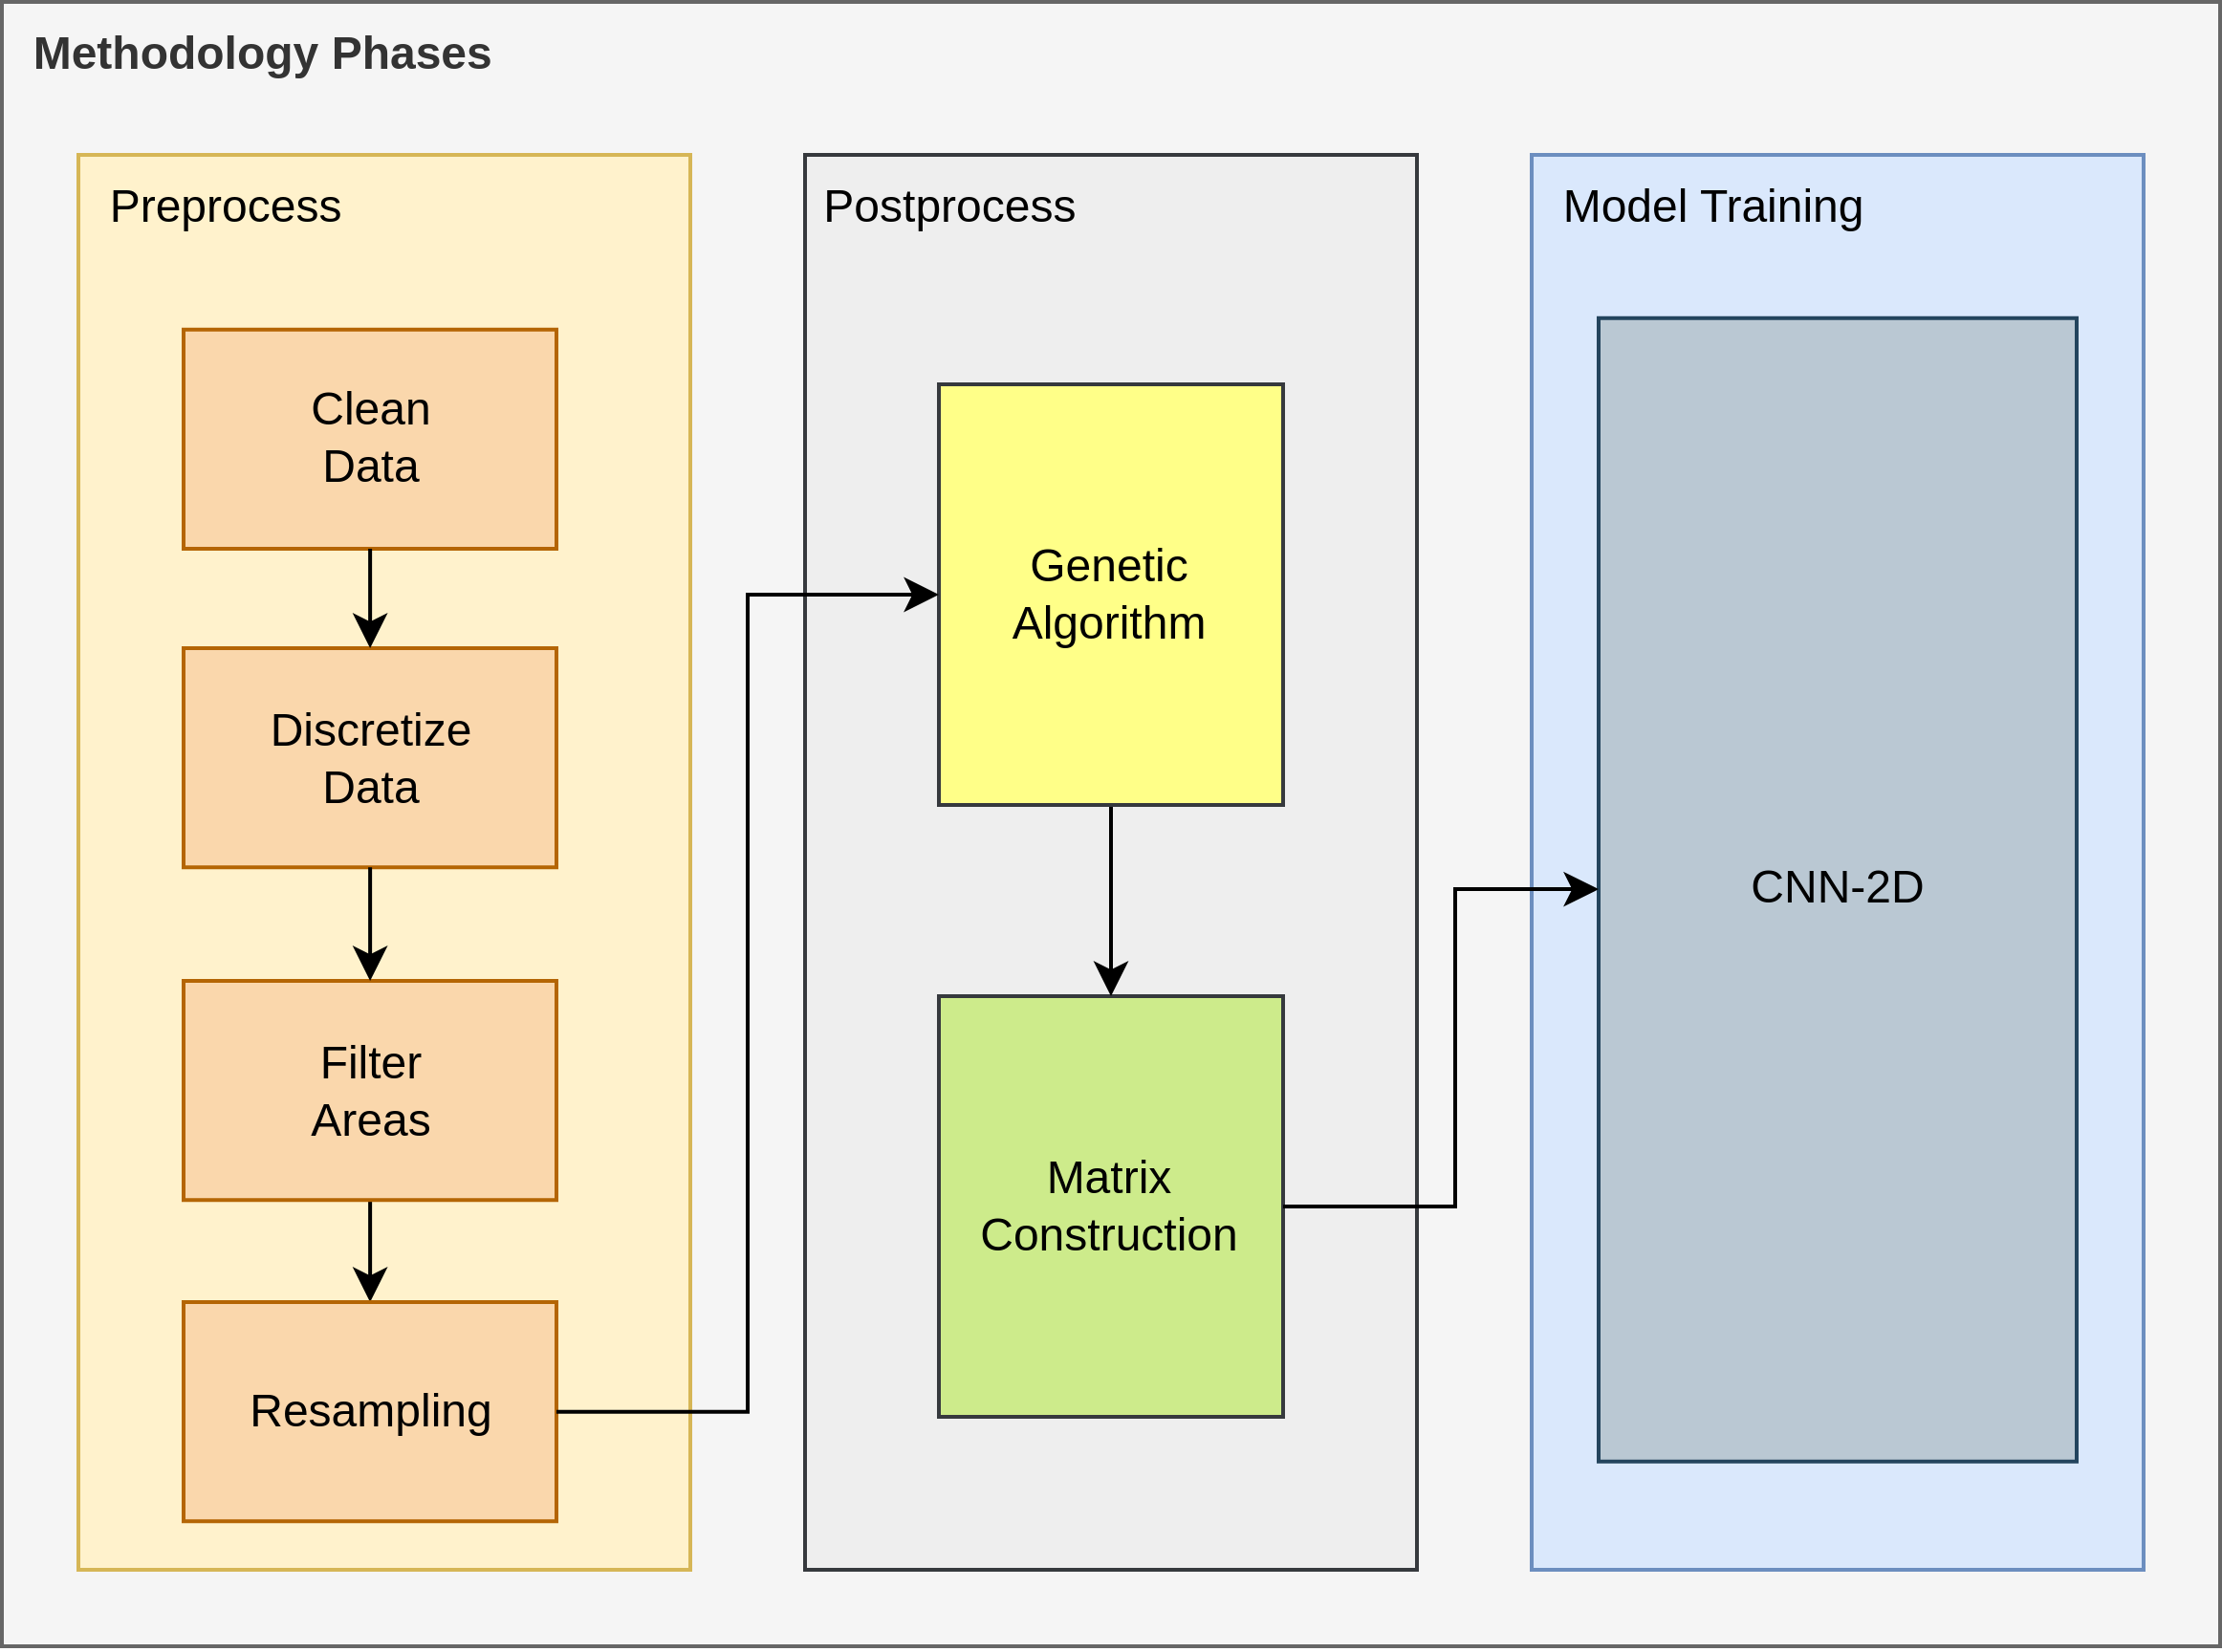
\includegraphics[width=14cm]{Figures/7th DataFlow Chart.png}
	\caption[Diagrama de flujo del modelo GTAAF]{Diagrama de flujo del modelo GTAAF. Consta de tres fases simplificadas: pre-procesado de datos, postprocesado y entrenamiento del modelo}
	\label{DataFlow}
\end{figure}

En segundo lugar, el concepto de gravedad de los accidentes es reasignado de tres a dos clases, accidentes sin necesidad de asistencia y accidentes con necesidad de asistencia. Esto se debe a que el balance entre lo que aporta y lo que resta el distinguir tres clases de accidentes, se decanta claramente por esto último ya que, un modelo de clasificación, a medida que incrementa el número de clases, tiene más posibilidades de realizar predicciones erróneas, sobre todo si son clases minoritarias y existe una clase intermedia conflictiva entre ellas. Por este motivo se distinguen dos clases de accidentes: \textbf{Con Asistencia} y \textbf{Sin Asistencia}.

Como tercera consideración, para paliar aún más el efecto del desbalanceo presente en los datos se diseña una técnica para balancear el dataset en base a la clase minoritaria aplicando un filtrado de áreas. Esta técnica tiene como objetivo dividir el mapa de la población en celdas, para seleccionar aquellas zonas de la región donde existan ambos tipos de accidentes. Con esto se consigue que la información interpretada por los modelos no se vea condicionada por la naturaleza de los mismos.

Para aportar más información, se añaden transformaciones sobre los datos en base a las variables ya existentes. Así, para capturar la naturaleza periódica de la hora del accidente se representó mediante dos componentes cíclicas utilizando funciones seno y coseno. 
%\textcolor{green}{MANU: está el párrafo acabado? Lo digo por la coma sospechosa tras coseno...}

%\textcolor{orange}{\textbf{Luis: } Coma quitada}

% \textcolor{blue}{\textbf{Luis: no dices nada de la categorización en el modelo preeliminar creo, tienes que mencionarlo}}

Como quinta variación a considerar, se redefinen las categorías donde son asignadas las características, pasando de cinco a seis posibles categorías finales. Con este cambio, se busca una reorganización que facilite la asignación de características a conceptos más generales que representan estas categorías. Esto implica que la definición de las matrices que se construyen pasan de tener una posible dimensión de $5\times5$ a $6\times4$, sobre estos conjuntos de datos siempre y cuando se dispongan características para contemplar las nuevas categorías.

Por otra parte, se han centrado los esfuerzo en desarrollar el modelo convolucional de dos dimensiones CNN-2D. Esto se debió al análisis de entrenamiento de los modelos CNN-1D y CNN-2D, optando por descartar el primero debido a la poca capacidad de generalización sobre el conjunto de validación ofrecido por el modelo unidimensional.

Por último, en un intento de evaluar la generalización del modelo propuesto, se ha probado en distintos datasets y áreas, ampliando los conjuntos de datos sobre los que se aplica la metodología. De esta forma, se incluyendo seis regiones de Reino Unido, una de Australia y Madrid. Además, se ampliaron los modelos del estado del arte contra los que comparar el rendimiento, llegando a seis, \textit{SVC, Naive Bayes, Bagging Random Forest, KNN, Regresión Logística} y una red neuronal Perceptrón Multicapa (\textit{MLP}).

\subsection{Pre-procesamiento}

Esta sección explica las diferentes etapas que componen la fase de pre-procesamiento de la metodología GTAAF propuesta. En esta etapa es donde se les aplica transformaciones a los datos para obtener a un conjunto de datos refinado e interpretable para cualquier modelo que trabaje con datos en formato tabular. 

Esta etapa está compuesta por cuatro fases: (1) proceso de limpieza de datos, donde se identifican, corrigen y se tratan las inconsistencias sobre los datos, (2) la discretización, donde se convierten las variables continuas en variables discretas y se codifican los valores cualitativos de las características, (3) el filtrado de áreas, donde se reduce el desbalanceo de los datos escogiendo subregiones de la ciudad donde se localicen ambos tipos de accidentes, y (4) el remuestreo, donde se se generan muestras sintéticas de la clase minoritaria para disponer de un dataset balanceado. En la Figura \ref{PreprocessingStage} se muestra el flujo sobre el que pasan los datos para cada una de las diferentes fases que componen la etapa de Pre-procesamiento. Esta figura será referenciada en las siguientes subsecciones en la explicación de las fases de Pre-procesamiento.

\begin{figure}[H]
	\centering
	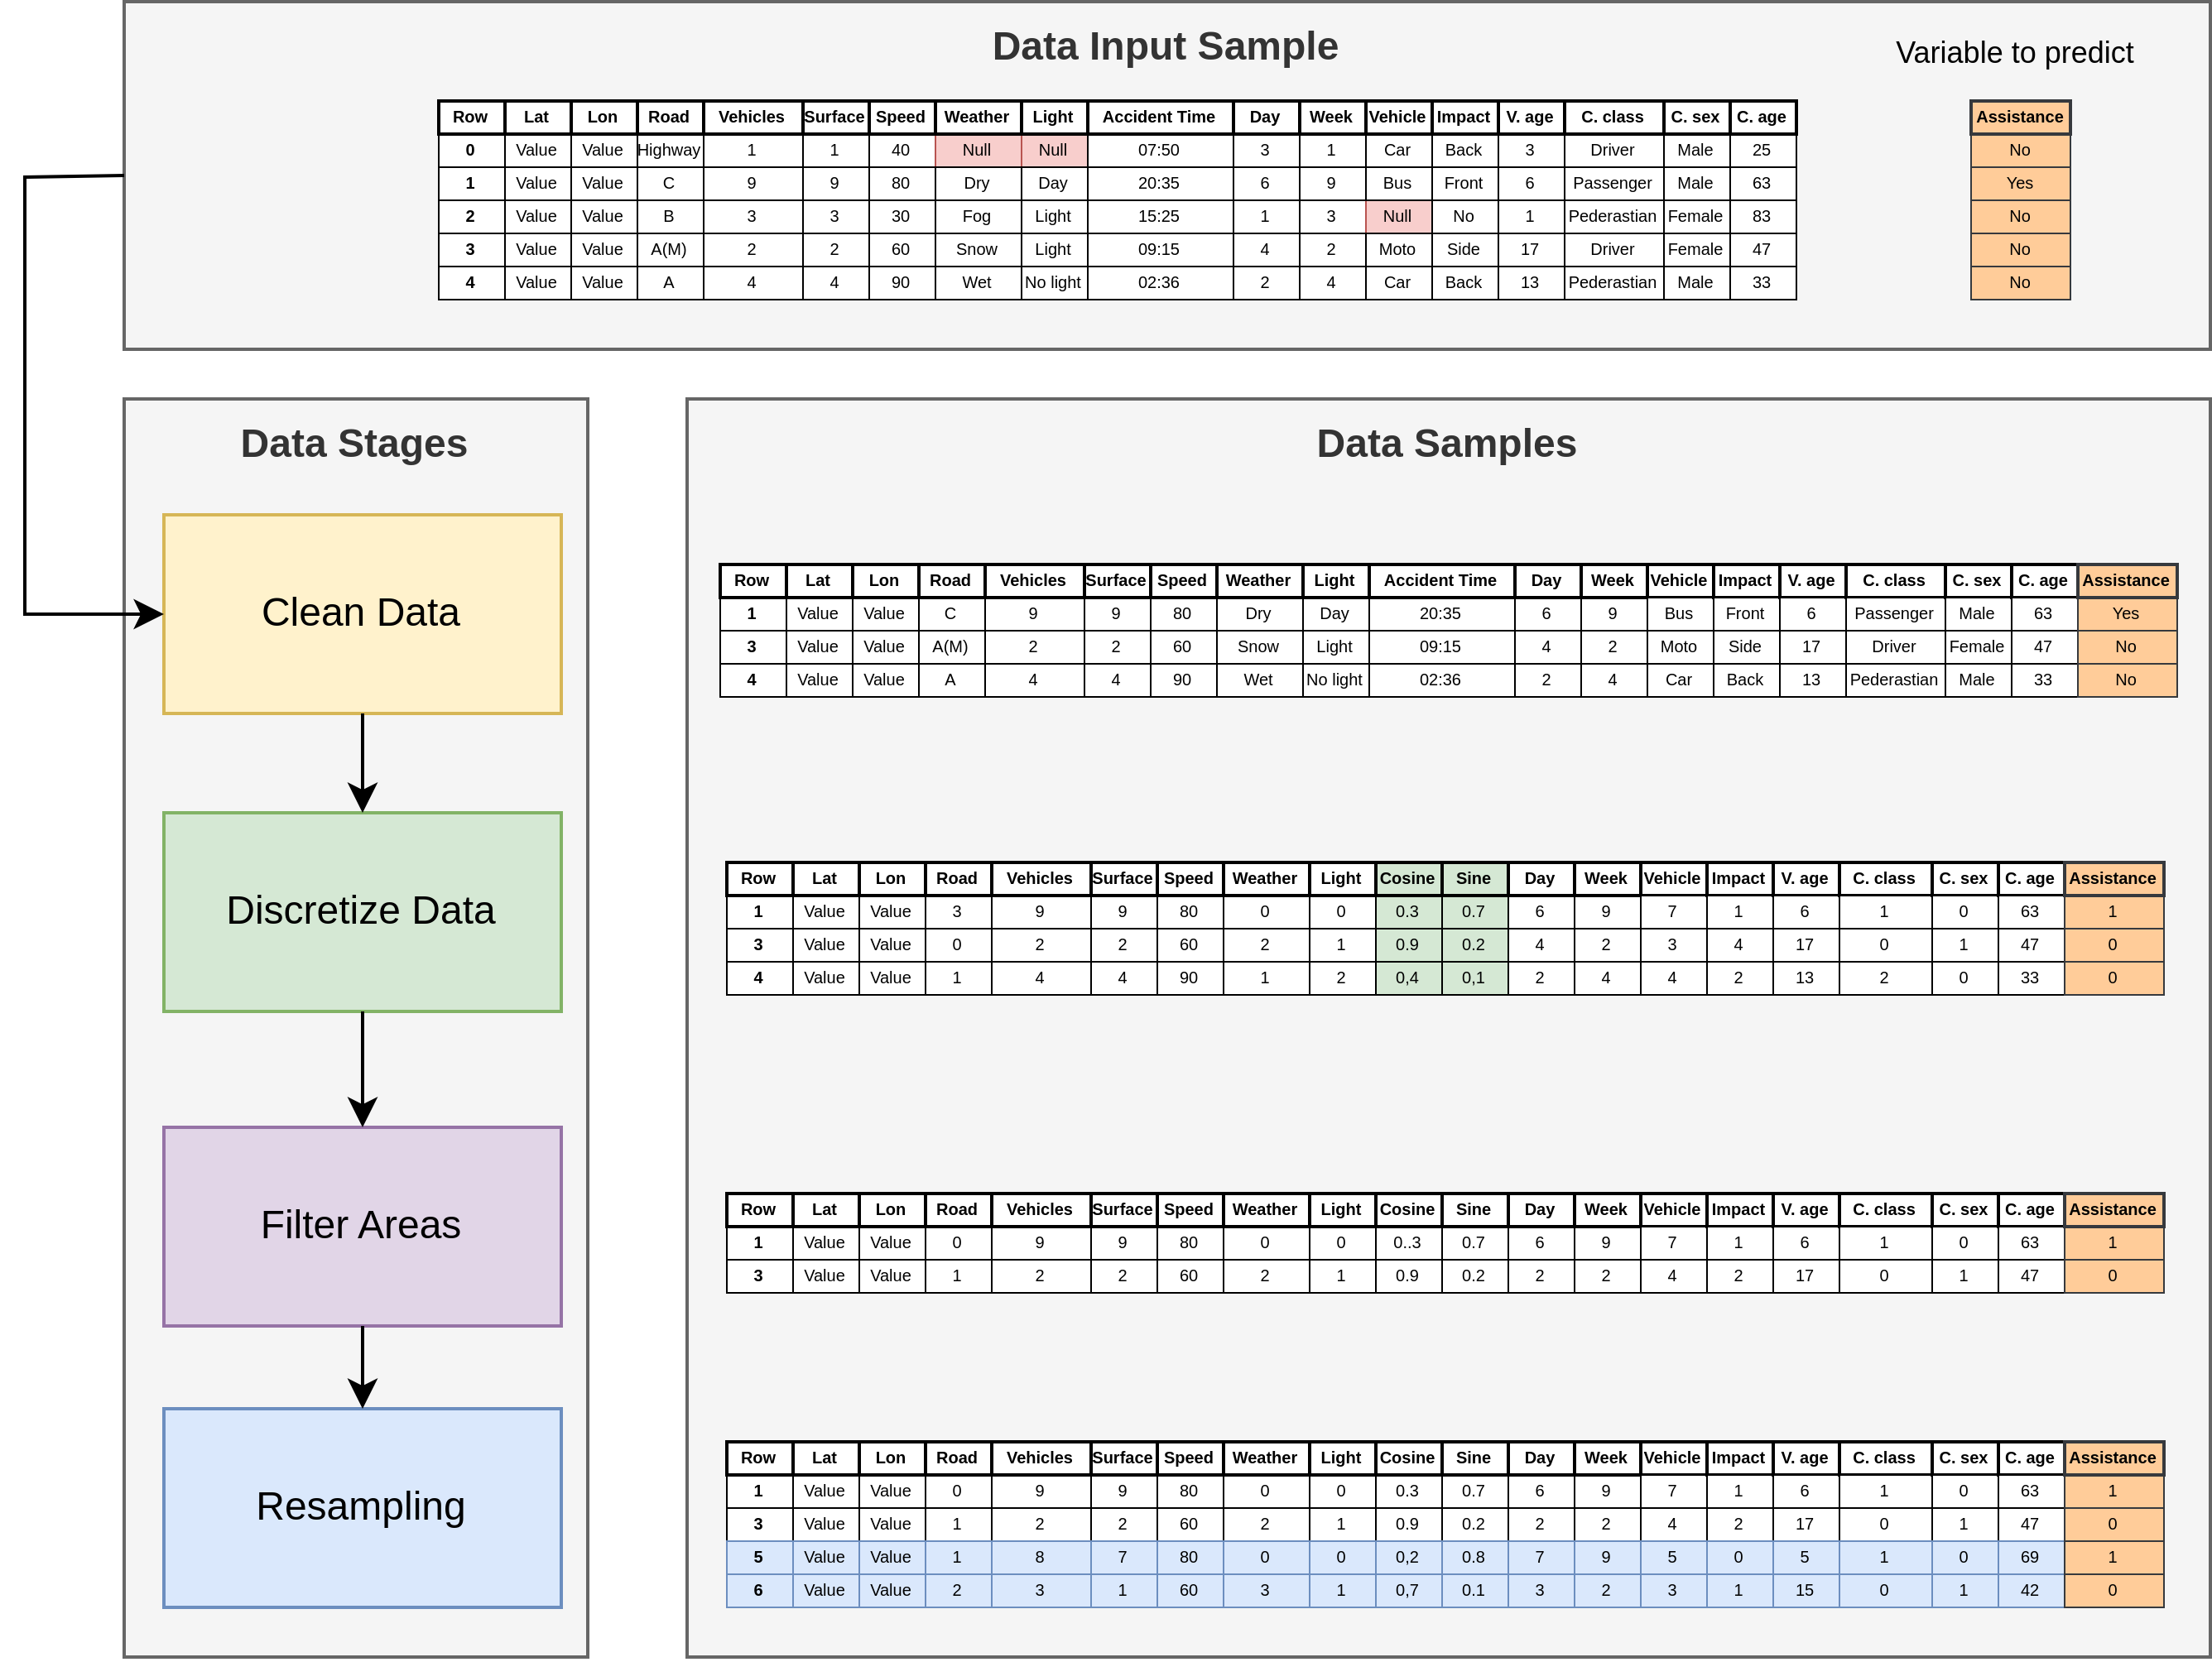
\includegraphics[width=14cm]{Figures/Preprocessing.png}
	\caption[Diagrama de flujo del Preprocesamiento de la metodología GTAAF] {Diagrama de flujo del Preprocesamiento de la metodología GTAAF. Consta de cuatro fases: (1) limpieza, (2) discretización, (3) filtrado de áreas y (4) \textit{resampling}}
	\label{PreprocessingStage}
\end{figure}

\subsubsection{Limpieza}

La limpieza de datos es un proceso esencial en cualquier proyecto de análisis de datos o inteligencia artificial. Esta fase tiene como objetivo tratar los datos de tal forma que el dataset procesado no disponga de valores ausentes, atípicos, presenten inconsistencias o errores. Este proceso asegura que los datos estén listos para análisis y modelado. Un conjunto de datos limpio y refinado es la base para comenzar a trabajar con modelos predictivos, ya que de otra forma los datos pueden no llegar a ser fiables debido a la incertidumbre presente en ellos \cite{ilyas2019data}.

La primera fase de la metodología contempla un proceso de limpieza, en el que aquellos registros de los datos que presenten valores nulos o aquellos que se muestren atípicos sobre las variables escogidas serán eliminados del dataset. Esto provoca que haya un porcentaje de los datos que son eliminados. Estos casos se encuentran representados de color rojo en la primera etapa de la figura \ref{PreprocessingStage}-naranja, donde los registros de accidentes con identificador $0$ y $2$ son eliminados del conjunto de datos al presentar valores vacíos en alguna de las características de interés seleccionadas.


\subsubsection{Discretización}

Los modelos predictivos trabajan con datos numéricos, que son los que están diseñados para interpretar, sobre los que realizan operaciones matemáticas para adquirir conocimiento y poder realizar inferencias sobre muestras nunca antes vistas. Es por esto que las características ofrecidas en los conjuntos de datos deben ser transformadas a estos valores sin perder el utilidad que representa la información. A la hora de describir un accidente, gran parte de la información que se obtiene tiene una naturaleza cualitativa y/o descriptiva. Esto se puede intuir de forma clara con el ejemplo de una característica que describa el punto de impacto del accidente, donde los valores que esta variable pudiera tomar se refiriesen a una descripción cualitativa del punto de impacto del vehículo, como pudieran ser: frontal, lateral o por alcance, entre otras. Por este motivo es necesario aplicar un proceso de cuantificación y discretización que busque transformar estos valores descriptivos en valores numéricos, de tal forma que los datos puedan ser interpretados por los modelos. Se busca representar de forma jerárquica la importancia de cada uno de los posibles valores descriptivos asignando un valor numérico que contemple la importancia ascendente de cada descripción, teniendo como objetivo que la información descriptiva contenida sea coherente con su representación numérica.

% Por este motivo, en esta sección se expondrán el proceso que se ha seguido para transformar las variables cualitativas a cuantitativas, realizando una propuesta de cuantificación en la que se asigna un valor numérico a cada variable en función de la importancia dentro del total de valores que cada una de estas puede contener.

En este trabajo se ha seguido un procedimiento de discretización incremental, donde a cada posible valor del conjunto de datos se le ha asignado un valor numérico en función de la importancia que se le ha asignado, véase \ref{PreprocessingStage}-verde.

%\textcolor{green}{MANU: corregidme si me equivoco, pero en este apartado dijimos que no deberían salir nombre de caracteristicas como aparecen en los datasets, sino mas genérico tipo 'donde los valores que esta variable pudiera tomar se referirían a una descripción cualitativa del punto de impacto del vehículo, como podrían ser frontal o lateral, por ejemplo.'}

%\textcolor{orange}{Luis: había puesto los valores, lo cambiado}

\subsubsection{Transformación (Sin/Cos)}

%\textcolor{blue}{\textbf{Luis: esto yo creo que estaría, a la espera de poner más bonito el dibujo.}}\\

Como se ha comentado anteriormente, los modelos de inteligencia artificial y aprendizaje estadístico interpretan los datos en forma numérica. El valor numérico que se le asigna a cada campo es crítico, ya que será así como el modelo interprete el orden de los valores cualitativos que los humanos somos capaces de comprender. La representación del formato de la horas y minutos del día, por su naturaleza, no es una excepción. El concepto de la hora del día tiene un componente cíclico que es necesario representar para que el modelo comprenda que las 11:59 de la noche es una hora muy próximas a las 00:00. Esto es algo a lo que los seres humanos estamos acostumbrados, pero debe ser indicado de forma coherente para los modelos de inteligencia artificial que interpretarían que estas dos horas muy parejas son valores totalmente opuestos en el rango numérico que puede contener la característica con el formato 24 horas que conocemos. Con el objetivo de representar de forma consistente la información de la hora del accidente, es necesario aplicar una transformación que interprete las horas y minutos en formato 24h a un formato cíclico, y para ello se transformará este campo inicialmente de una dimensión, a dos dimensiones sinusoidales. Para realizar este proceso en primer lugar se transforma la hora y el minuto en el que se ha producido cada accidente a segundos. Posteriormente se aplican las siguientes fórmulas sobre los segundos para representar la hora del accidente en dos componentes, el senosoidal y el cosenoidal (ecuaciones \ref{SIN_EQUATION} y \ref{COS_EQUATION} respectivamente).


\begin{equation}
	\sin((2 \cdot \pi \cdot DaySeconds)/SecondsInDay)
	\label{SIN_EQUATION}
\end{equation}
\begin{equation}
	\cos((2 \cdot \pi \cdot DaySeconds)/SecondsInDay)
	\label{COS_EQUATION}
\end{equation}

%(Dibujito explicativo de senos y cosenos)[puedo poner las 23:59 de la noche representada en seno y coseno, las 00:00 y las 15:00 para que se vean las diferencias].

En la figura \ref{HoursPlot} se muestra un ejemplo de la naturaleza cíclica de la representación de la variable Hora en forma de seno (eje de ordenadas) y coseno (eje de coordenadas), donde se observa que la hora 22:20 en el espacio bidimensional se encuentra más cercana a la hora 01:45 respecto a cualquier otra posible representación unidimensional.

\begin{figure}[h]
	\centering
	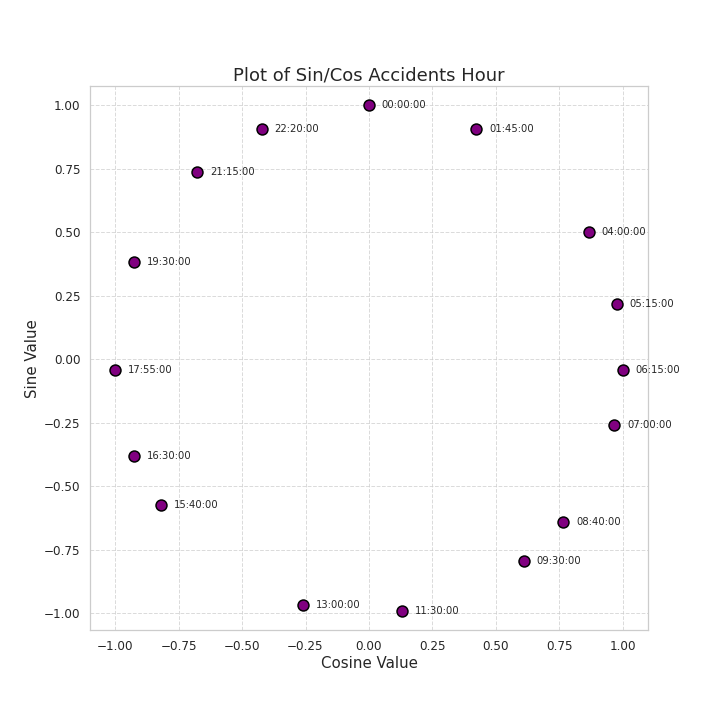
\includegraphics[width=10cm]{Figures/normal_plot.png}
	\caption{Representación de las horas en formato de seno y coseno}
	\label{HoursPlot}
\end{figure}

Esta transformación sobre los datos puede apreciarse en el diagrama de flujo de Preprocesado \ref{PreprocessingStage}-verde, donde se incluyen las nuevas componentes temporales y se elimina la hora del accidente.

\subsubsection{Filtrado de Áreas}

Uno de los retos más comunes en el campo de la inteligencia artificial es disponer de un conjunto de datos no balanceado. Este problema implica tener una desproporción del número de muestras en base a la variable a predecir. Esta casuística afecta negativamente al entrenamiento de los modelos, ya que estos en su etapa de entrenamiento adquieren el conocimiento prediciendo sobre estas muestras y son penalizados cuando sus predicciones durante esta fase son erróneas. Si la distribución de datos de entrenamiento dispone de muchas más muestras de una clase que de otra, el modelo tenderá a aprender durante su entrenamiento a predecir siempre aquella clase mayoritaria, ya que se le ha penalizado en menos ocasiones durante esta fase, obteniendo así un modelo sesgado que está condicionado por naturaleza a predecir sobre la clase más común.

En lo que respecta la naturaleza de la distribución de datos de accidentes de tráfico, siempre existirán muchos más accidentes que no han necesitado asistencia respecto a los que sí. Por lo que durante esta fase de la metodología se busca paliar este efecto tratando de reducir la diferencia entre el número de registros de la clase mayoritaria (sin necesidad de asistencia) y la clase minoritaria (necesidad de asistencia).

Para solventar esto se aplica un filtrado basado en áreas, que buscará balancear los datos escogiendo áreas estratégicas donde coexistan accidentes con ambos tipos de consecuencias. Para cada población se establece una ventana de dimensiones (\textit{X,Y}) que recorrerá secuencialmente el área total que engloba cada una de las regiones escogidas en esta tesis. Esta ventana buscará si en ese área coexisten accidentes de tipo No-Asistencia y Asistencia, de tal forma que si esto se cumple, dicha subárea se mantendrá en el dataset, y en caso contrario se eliminará. Esto consigue un balanceo de los datos que minimiza el número de accidentes de tipo No-Asistencia en el dataset que no sean estrictamente necesarios. En la figura \ref{Areas} se muestra un ejemplo del criterio seguido para aplicar este filtrado, donde se seleccionan únicamente aquellas regiones donde coexisten accidentes sin necesidad de asistencia (verde) y con necesidad de asistencia (rojo).


\begin{figure}[H]
	\centering    
	\subfloat[Ejemplo de muestras de accidentes originales]{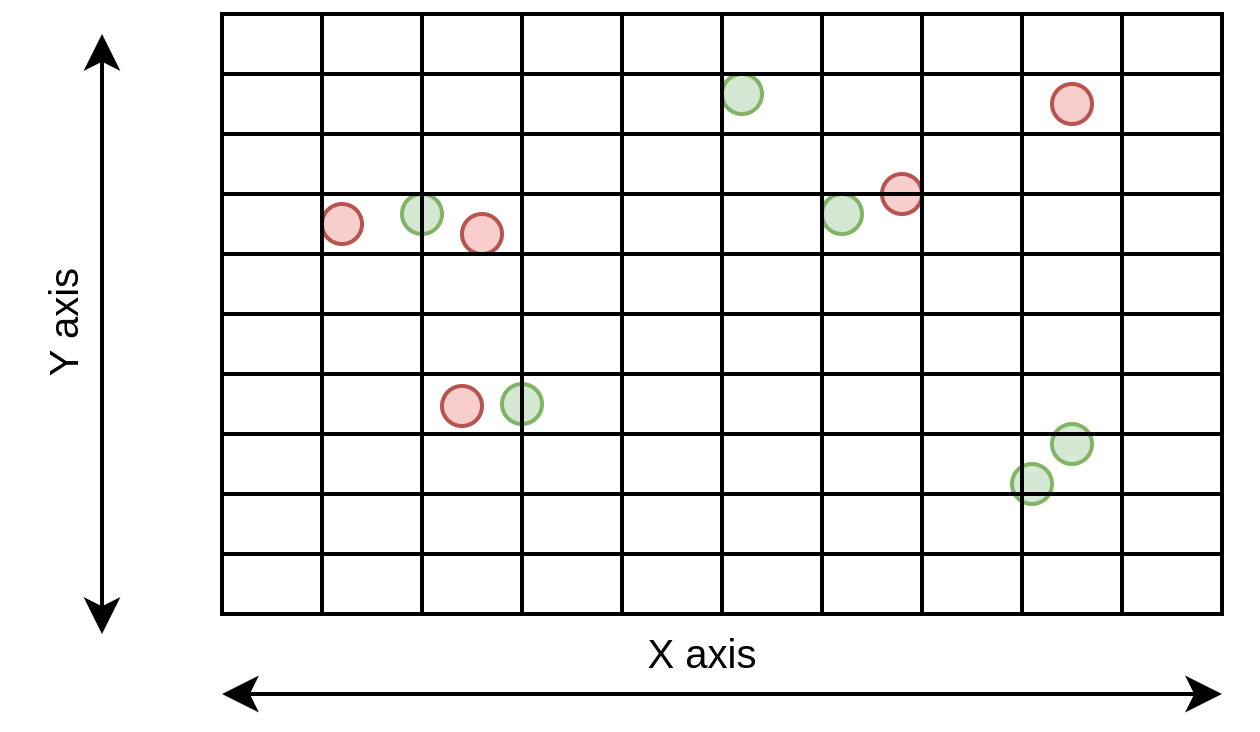
\includegraphics[width=7cm]{Figures/areas-points.png}}
	\subfloat[Ejemplo de muestras de accidentes filtradas]{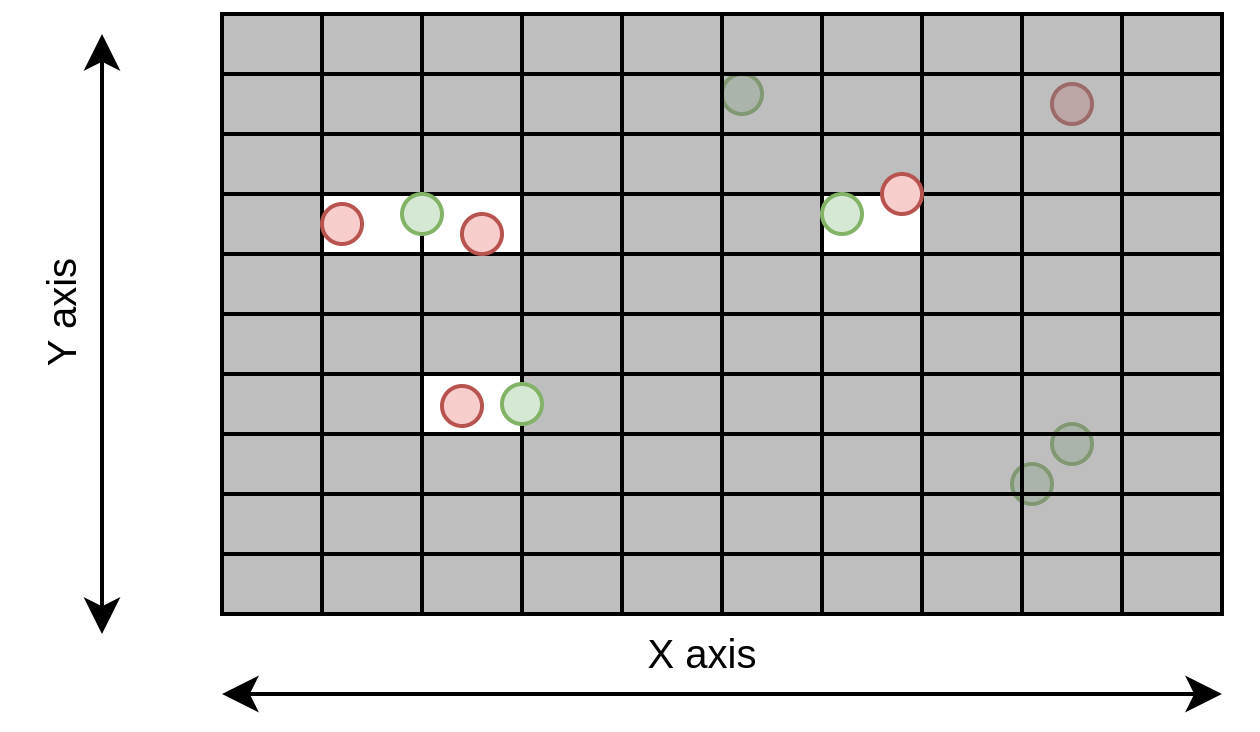
\includegraphics[width=7cm]{Figures/areas-points-filtered.png}}
	\caption[Ejemplo de filtrado de áreas]{Ejemplo de filtrado de áreas. Los puntos verdes representan accidentes que no requieren asistencia, mientras que los puntos rojos representan accidentes que necesitan asistencia}
	\label{Areas}
\end{figure}

En la Figura \ref{PreprocessingStage}-morado se muestra el ejemplo donde el accidente sin necesidad de asistencia con identificador $4$ se elimina del conjunto de datos porque no convive con otro accidente de tipo asistencia dentro de su mismo área.

\subsubsection{División de datos}

%\textcolor{blue}{\textbf{Luis: esto yo creo que estaría, lo único hacer inciso en lo último.}}\\

Los modelos supervisados de inteligencia artificial aprenden patrones sobre datos que son ofrecidos en la etapa de entrenamiento del modelo. Durante esta fase los modelos realizan predicciones sobre de datos y posteriormente se les enseña la clase a la que pertenecía cada uno de los datos que ha predicho, de esta forma se mide el error que han cometido durante este proceso y los pesos de la red son actualizados para minimizar el error en la siguiente fase. Si este aprendizaje se repite durante muchas etapas, el modelo tiende a aprender los datos de memoria, lo que se conoce como sobreajuste de la red u \textit{overtfitting}, provocando que la red no sea capaz de generalizar ante nuevas muestras tras su entrenamiento. Por este motivo es importante mantener el control del aprendizaje de la red mediante la evaluación de su rendimiento en cada época de entrenamiento mediante un conjunto de datos que nunca ha visto durante su fase de aprendizaje, este conjunto de datos es conocido como conjunto de validación, y es utilizado como referencia para limitar el entrenamiento cuando el modelo no sea capaz de generalizar sobre estas nuevas muestras. Por otra parte, existe un conjunto de datos de test, utilizado para medir el rendimiento del modelo final una vez ha acabado su fase de aprendizaje. Este conjunto pertenece a muestras que la red no ha visto durante su fase de aprendizaje ni ha sido utilizado como validación.

En este trabajo se ha dividido el conjunto de datos original de cada una de las ciudades mediante el porcentaje $80\%$ para entrenamiento y $20\%$ para validación y test.


\subsubsection{Resampling}

Una vez se disponen de los datos refinados, es necesario aplicar algún proceso que logre balancear los datos en función de la clase a la que pertenecen. El conjunto de datos, una vez se han reducido considerablemente el desbalanceo entre las dos clases gracias al proceso de filtrado de áreas, sigue presentando cierto desbalanceo. Por mucho que se haya acotado el problema a regiones individuales, es lógico que se hayan producido más accidentes sin necesidad de asistencia respecto a los que sí la requieren.

En el caso de estudio de esta tesis, aplicar técnicas de \textit{Undersampling} que eliminen accidentes sin necesidad de asistencia hasta igualar el número de aquellos que sí la requieren es un inconveniente, ya que al disponer de tan pocas muestras de la segunda clase, el conjunto de datos resultante se vería notablemente reducido y afectaría negativamente al entrenamiento de la red que requiere de un conjunto de datos lo más extenso posible para favorecer la generalización en sus predicciones.

Por este motivo, se opta por métodos de aumentado de datos (\textit{Upsampling}), que mantienen el valor que aportan las muestras de los accidentes sin necesidad de asistencia, aumentando los datos de aquellos que sí la requieren. Se ha optado por una técnica de generación de datos sintética denominada \textit{Synthetic Minority Oversampling Technique (SMOTE-II)}, que busca incrementar el número de clases de las muestras minoritarias mediante la generación de nuevas muestras artificiales.

En la Figura \ref{PreprocessingStage}-azul se observan, marcados en azul, cómo los registros con identificadores $5$ y $6$ han sido generados en base a las modificaciones de los valores de los registros $1$ y $3$ para balancear el dataset.



\subsubsection{Normalización}

En cualquier modelo de inteligencia artificial es imprescindible normalizar los datos. Los modelos predictivos trabajan con valores numéricos realizando operaciones sobre ellos. En los conjuntos de datos suelen coexistir variables cuyos valores se encuentran representados en distintas escalas, es decir, que los valores que pueden tomar ciertas características suelen presentar un rango de valores mucho más amplio que otras de ellas dentro del mismo conjunto de datos, haciendo que las características sean incomparables entre sí debido a la diferencia entre su magnitud. Un ejemplo de esto puede observarse en una característica que pudiera describir la semana dentro del año en el que se ha producido el accidente y, por otra parte, el sexo de la víctima. La primera de estas variables puede contener un amplio rango de posibles valores (desde el $0$ hasta el $51$), en función de la semana en la que se ha producido el accidente, mientras que la segunda variable únicamente puede tomar dos valores ($0$ ó $1$). Esta diferencia numérica en los posibles valores de los datos provoca que las operaciones matemáticas que aplican los modelos durante su fase de entrenamiento sean desproporcionadas en las características con rango de valores más altos, produciendo una desproporción en estas operaciones y provocando que los datos incomparables entre sí, dándole más importancia a unas características que a otras. Es por esto por lo que es necesario un proceso de logre acotar el rango de posibles valores del conjunto total de datos para poder operar sobre todos los descriptores con la misma importancia. Existen distintas técnicas para aplicar la normalización en los datos, como \textit{Mean Centered (MC)}, \textit{Variable Stability Scaling (VSS)} o \textit{Min-Max Normalization (MMN)}, entre otras \cite{DataNormalizationInvestigation}. En este trabajo para normalizar los datos y hacerlos comparables entre sí se ha utilizado la técnica de \textit{Z-Score (ZSN)} (ecuación \ref{Z_SCORE_EQUATION}) debido a que logra representaciones de acuerdo con una distribución normal. Para hacerlo, se utilizan la media y la desviación estándar para reescalar los datos de manera que su distribución esté definida por una media de cero y una desviación estándar unitaria.

\begin{equation}
	\label{Z_SCORE_EQUATION}
	Z = \frac{(X - \mu)}{\sigma}
\end{equation}




\subsection{Post-procesamiento}

La segunda fase de la metodología implica transformar los datos refinados y balanceados en matrices interpretables por el modelo GTAAF propuesto. Este proceso conlleva asignar los atributos de las muestras tabulares en posiciones dentro de estas matrices. Para realizar esto, se hace uso de un método de transformación que toma en consideración la importancia de cada característica dentro del conjunto de datos. El objetivo es posicionar estratégicamente las características más relevantes en la matriz para maximizar su impacto en el modelo GTAAF, como se ilustra en la Figura \ref{PostprocessingStage}. La determinación de la importancia de las características se basa en un algoritmo tipo boosting, \textit{XGBoost}, que asigna pesos a las variables según su relevancia en la separación de datos durante el entrenamiento de este. Para garantizar un entrenamiento óptimo del modelo, se realiza una optimización de hiperparámetros utilizando algoritmos evolutivos. A lo largo de generaciones sucesivas, este algoritmo genético hace evolucionar los hiperparámetros, guiado por la métrica de \textit{F1-Score}, que actúa como función heurística a optimizar.

\begin{figure}[H]
	\centering
	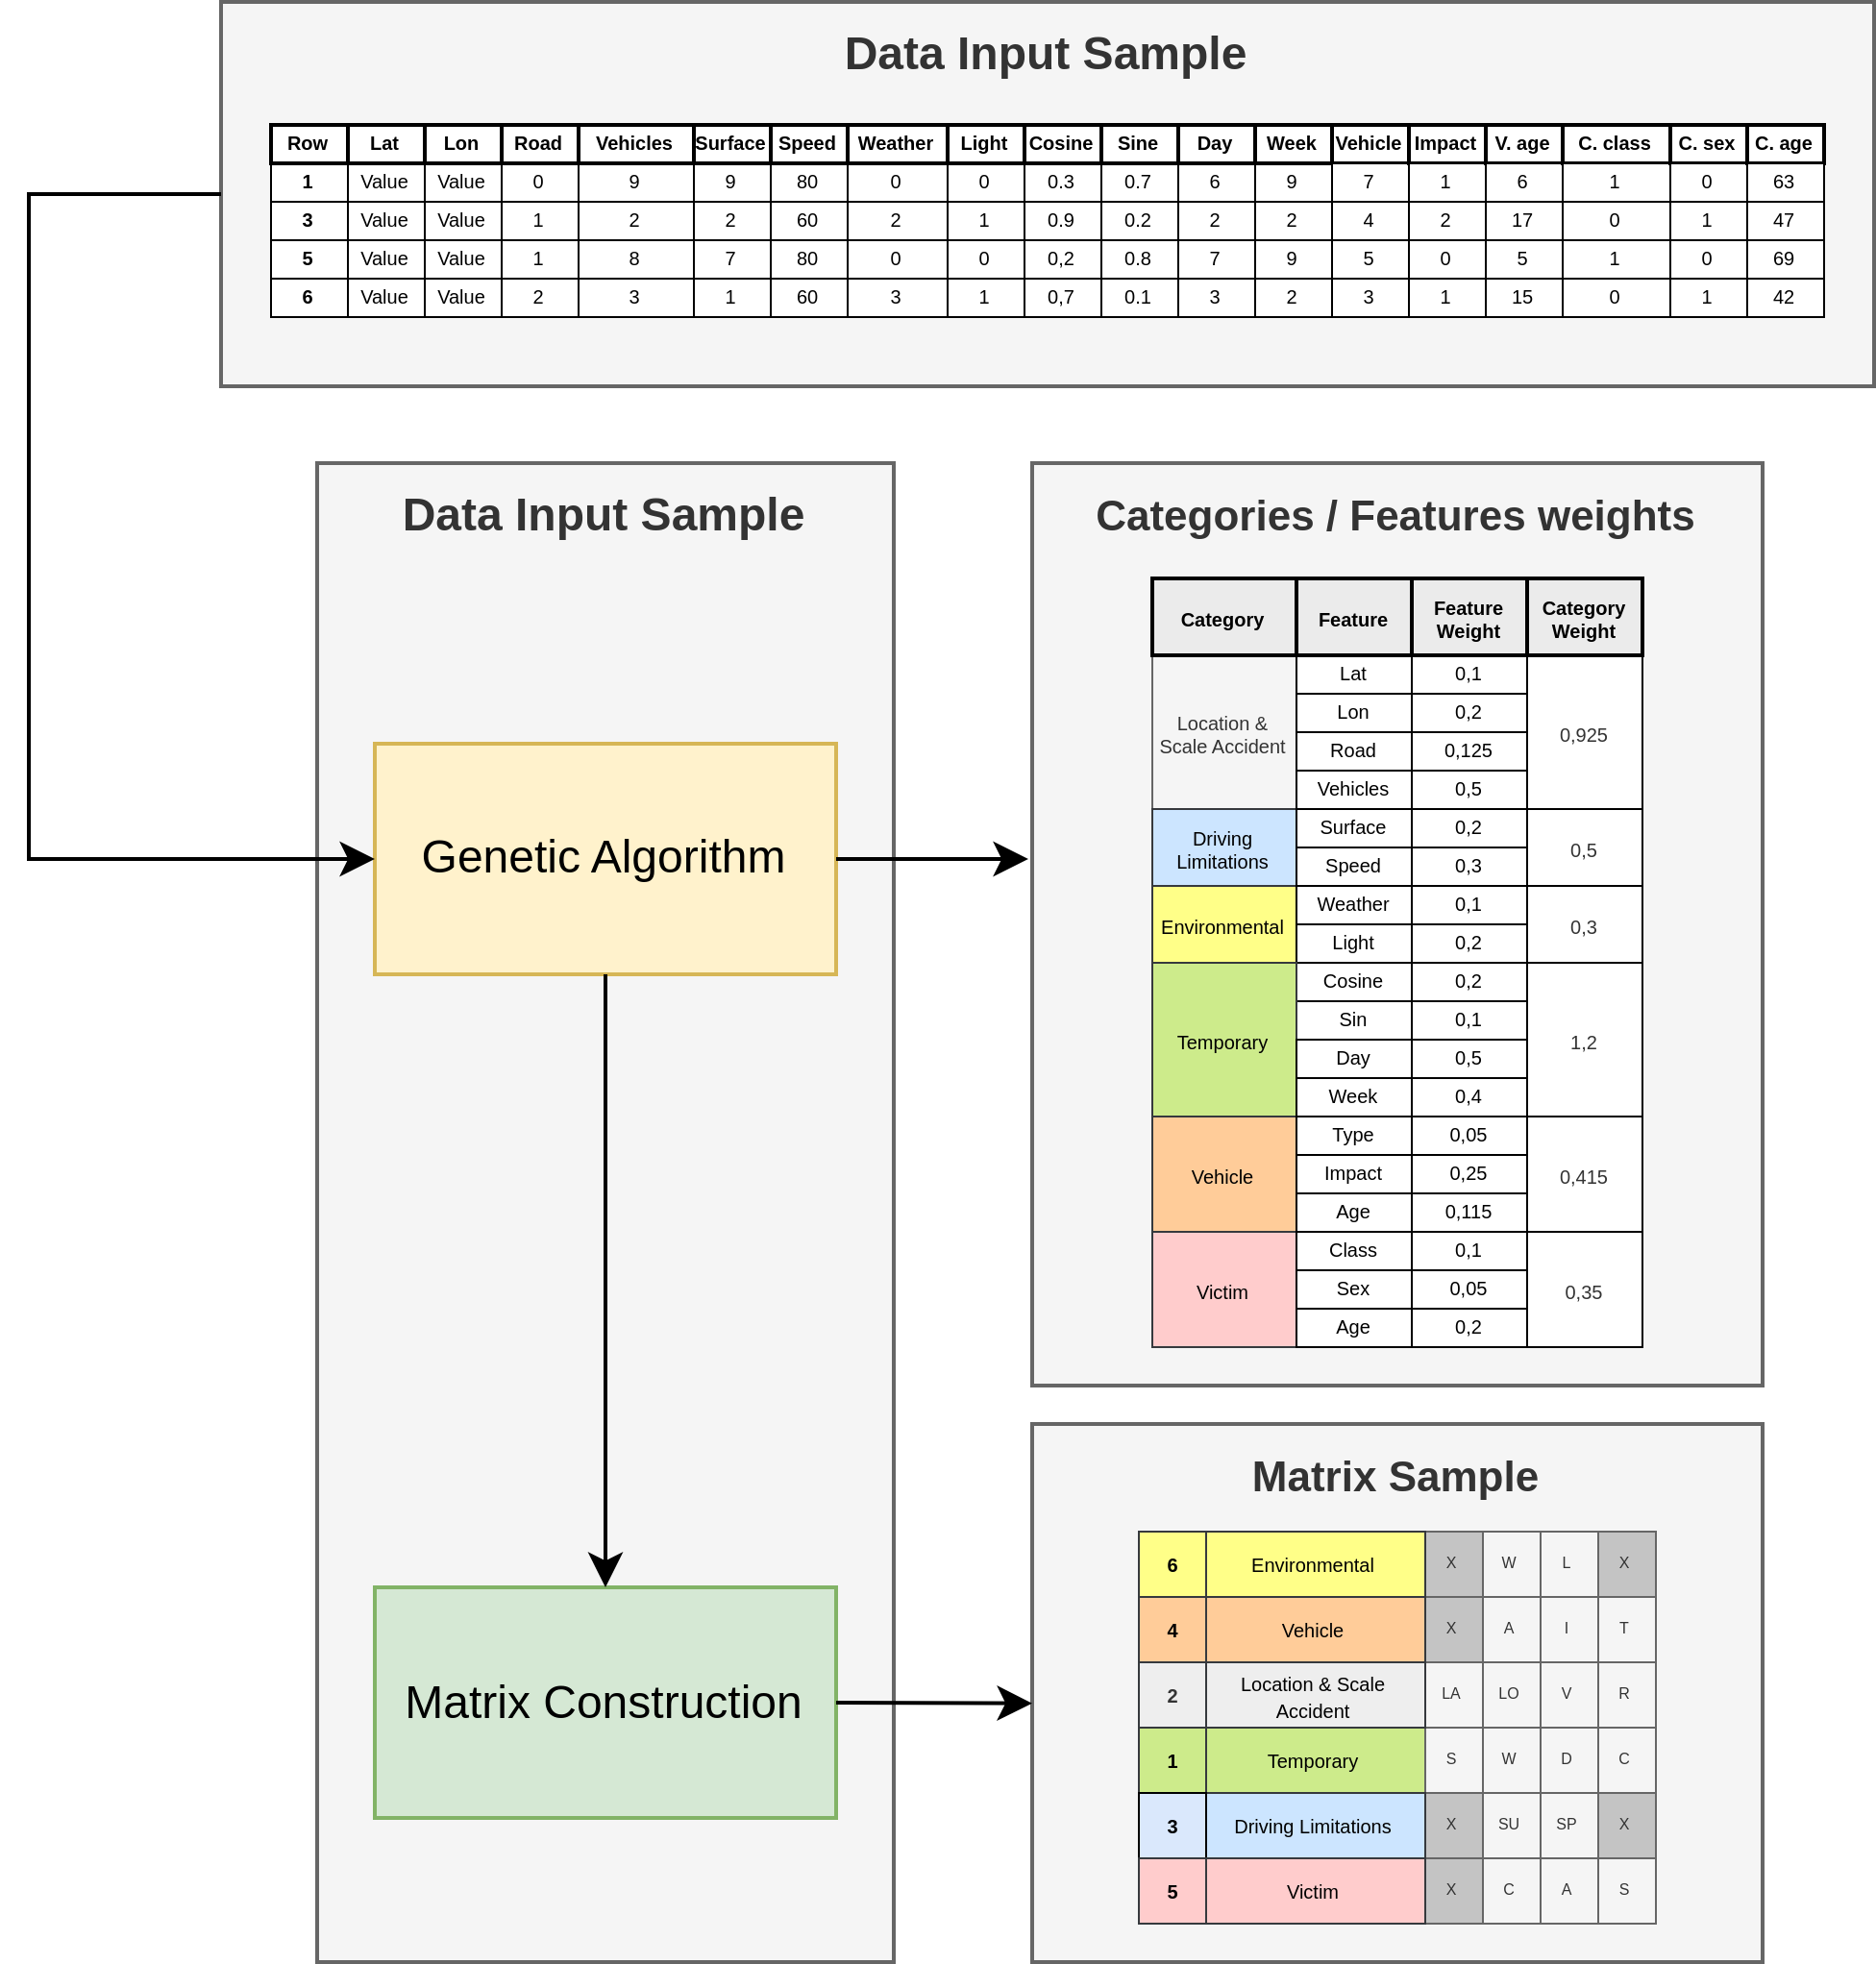
\includegraphics[width=14cm]{Figures/Postprocessing_2.png}
	\caption[Diagrama de flujo del Postprocesamiento de la metodología GTAAF]{Diagrama de flujo del Postprocesamiento de la metodología GTAAF. Consta de dos fases: (1) aplicación del algoritmo genético para la optimización de hiperparámetros de \textit{XGBoost}, y (2) construcción de matrices en base a los pesos de las categorías}
	\label{PostprocessingStage}
\end{figure}

\subsubsection{Construcción de Matrices}

En este trabajo, se presenta un método para transformar datos, inicialmente tabulares, a datos matriciales con los que podrá trabajar el modelo GTAAF. Esta transformación hace uso de la categorización de las características y la importancia de cada una de ellas individualmente dentro del conjunto de datos a las que pertenecen. En secciones anteriores se ha explicado el funcionamiento del proceso de categorización propuesto, que busca poder aplicar esta metodología a cualquier conjunto de datos de accidentes, agrupando las características en conceptos básicos y de fácil obtención. El siguiente paso para lograr la transformación de los datos, inicialmente en filas y columnas, a datos matriciales es asignar cada una de las características del conjunto de datos a una posición dentro de la matriz, de tal forma que los datos puedan ser interpretados por el modelo convolucional. Para tener un contexto de la importancia en el orden en el que se asignan estas características, se explica brevemente la intuición sobre la que trabajan las redes neuronales convolucionales. Los píxeles que componen una imagen representan patrones que, para los seres humanos, son reconocibles, las redes convolucionales aprenden a reconocer estas variaciones inicialmente en una escala pequeña (pocos píxeles) y, a medida que aumenta el número de capas de las que se componen estas redes son capaces de aprender patrones más complejos en base a la composición de aquellos más simples. Este funcionamiento, por definición, implica que la forma en la que se construye una imagen artificial sea crítica, es decir, que el contenido que representa la imagen debe estar formado de manera coherente para que las redes puedan aprender estos patrones, requiriendo un sentido y/o contexto completo en su composición.

Existen distintos métodos que logran transformar datos tabulares a una representación matricial de los mismos, buscando dar un sentido a la asignación de las características en posiciones de la matriz. En la sección \ref{SOAT_MATRIX_ALGORITHM_CONSTRUCTION} se presentaron distintos métodos como \textit{REFINED, DeepInsight} o \textit{IGTD}, que buscan optimizar la posición de las características en base a la similaridad que presenten entre ellas, principalmente en datos orientados a la descripción genética. Sin embargo, estas técnicas presentan distintas limitaciones debido a la magnitud de los datos para las que han sido diseñadas (del orden de $2500$ características), esto provoca que estos métodos sean difícilmente aplicables a datos de baja dimensionalidad, pudiendo asignar espacios en blanco ante la falta de características o que los métodos no sean capaces de converger al trabajar con tan pocos datos. En el caso de estudio de esta tesis las características disponibles son mucho menores, del orden de $20$ variables.

Debido a las limitaciones de los métodos anteriores, en este trabajo se presenta un método de composición de matrices en base a la importancia de las características, que permite asignar cada una de las variables del dataset a posiciones estratégicas dentro de la matriz haciendo uso de dos conceptos fundamentales: los algoritmos genéticos y los algoritmos de medición de importancia de características.

\subsubsection{Algoritmos de medición de importancia de características}
%\subsubsection{Feature Importance Algorithm}
\label{FEATURE_IMPORTANCE:ALGORITM_JUSTIFICATION}
%\textcolor{blue}{\textbf{Luis: Floja la justificación, pero van por ahí los tiros.}}\\

Como se ha presentado en la sección \ref{SOAT_FEATURE_IMPORTANCE_METHODS}, existen distintos métodos que permiten evaluar la importancia de las variables en función de distintos criterios, como la correlación que presentan las variables entre sí o el nivel de importancia de cada característica a la hora de entrenar un modelo predictivo. Ejemplos como estos son la Regresión Logística, técnicas de \textit{ensembles} de tipo \textit{Bagging} como los \textit{Random Forest} o métodos \textit{ensembles} tipo \textit{Boosting}.

En esta tesis se trabaja con conjunto de datos desbalanceados, por lo que a la hora de aplicar algoritmos de medición de características es importante escoger técnicas que sean insensibles a esto. Una de las muchas propiedades que ofrecen de los métodos de \textit{ensembles} es que se adaptan especialmente bien a conjuntos de datos sesgados. Estos modelos, en sus distintas formas, se benefician de estar compuestos de una combinación de modelos que, mediante distintas técnicas de muestreo, consiguen reducir considerablemente el sobreajuste que pueda darse con otros métodos.

Dentro de estos modelos, los \textit{ensembles} tipo \textit{Boosting} son ampliamente conocidos por adaptarse especialmente bien en estos casos. Estos modelos utilizan técnicas de regularización durante su entrenamiento y se centran en minimizar el error producido cuando clasifican muestras de aquellas clases más conflictivas, que en el caso de un dataset desbalanceado serían las muestras minoritarias. Por otra parte, son modelos muy robustos que generalmente ofrecen un mayor rendimiento respecto a otros tipos de \textit{ensembles} como los \textit{Random Forest}, que únicamente ofrece que cada uno de los modelos sea entrenado con un subconjunto de los datos originales.

En esta metodología se utilizará el algoritmo tipo \textit{Boosting XGBoost}, donde se minimizará el error del modelo mediante la métrica \textit{F1-Score} resultante de la clasificación de ambas clases de accidentes (sin necesidad de asistencia y con necesidad de asistencia).

Este algoritmo ofrece una serie de hiperparámetros, que permiten configurar el método para maximizar su rendimiento. Del total de hiperparámetros disponibles para su configuración, se escogerán aquellos más relevantes, concretamente la profundidad máxima que puede tomar el árbol, el número de árboles que minimizarán el error de sus predecesores y  la tasa de aprendizaje (\textit{learning rate}). Para ello se aplicarán técnicas de optimización de hiperparámetros basadas en algoritmos evolutivos.


% Existen múltiples algoritmos que implementan esta filosofía, entre los que destacan: (1) AdaBoost, orientado a clasificación, que en cada iteración , (2) Random Forest () y (3) XGboost. Para la metodología presentada en esta tesis se ha escogido la técnica XGBoost, ya que las características de este algoritmo son las más adecuadas a este contexto. XGBoost es menos sensible a datos que presentan una alta variabilidad y un importante desbalanceo entre ellos. Además, este algoritmo permite una mejor optimización en sus árboles sucesores al configurar los hiperparámetros con los que se entrena únicamente una única vez para el árbol inicial (profundidad del árbol, número de árboles y learning rate) [2]. El funcionamiento del XGBoost escogido es el siguiente...


\subsubsection{Algoritmo Genético}

Como se ha comentado en la sección \ref{HYPERPARAMETERS_OPTIMIZATION_METHODS}, existen numerosos métodos para optimizar hiperparámetros, cada uno con sus ventajas y desventajas dependiendo del contexto y los datos en el que se apliquen.

Debido a las limitaciones computacionales que supone la combinación de todos los posibles valores de los hiperparámetros, el método \textit{Grid Search} no se adapta adecuadamente al caso de uso contemplado en esta tesis. Por otra parte, siguiendo la línea de probar combinaciones de hiperparámetros sin una evolución en su convergencia, el método \textit{Random Search} aunque ses más eficiente que la búsqueda de cuadrícula, no es idóneo para este caso, ya que no sigue ningún patrón que explote las mejores soluciones que se van obteniendo, siendo estas combinaciones meramente aleatorias.

Debido a esto, en esta tesis se utilizan algoritmos genéticos para optimizar los hiperparámetros de entrenamiento del algoritmo \textit{XGBoost}. Este tipo de algoritmos permiten una exploración amplia del espacio de búsqueda de los hiperparámetros óptimos, acentuando además la explotación en soluciones cercanas al óptimo ideal. El algoritmo con los hiperparámetros optimizados \textit{XGBoost} ofrecerá la importancia de las características, necesaria para la construcción de las matrices de entrada al modelo GTAAF. Donde cada uno de los individuos de la población del algoritmo genético representará una posible combinación de hiperparámetros, concretamente los valores de (\textit{Max Depth}, \textit{ETA} y el número de árboles). La función heurística que será optimizada será el \textit{F1-Score} otorgado sobre los datos de test de cada uno de los conjuntos de datos.

\subsubsection{Construcción de Matrices}

Una vez se dispone de la categorización de los datos y de los pesos de las características gracias al modelo \textit{XGBoost}, se aplica el proceso de asignación de cada una de las variables a posiciones de la matriz. Como se ha comentado en secciones anteriores, la forma en la que se compone una matriz sobre la que opera una red convolucional es de vital importancia y por esto es necesario aplicar un método que logre transformar estos datos de manera coherente y eficiente. Existen diferentes enfoques para construir matrices en base a datos tabulares, pero estos enfoques como se ha comentado en la sección \ref{FEATURE_IMPORTANCE:ALGORITM_JUSTIFICATION} sufren de limitaciones aplicados a nuestro caso de uso, ya sea porque necesitan conocimiento del dominio o porque han sido diseñados para un número de características mucho mayor respecto a las disponibles en los conjuntos de datos de accidentes de tráfico. Para solventar estos inconvenientes se ha diseñado una estrategia que pretende posicionar las características más relevantes de cualquier conjunto de datos (definidas por el algoritmo \textit{XGBoost}) a posiciones cercanas al centro de la matriz, que son las zonas de importancia para los filtros de las redes convolucionales. Este proceso, teniendo en cuenta la categorización inicial que permite aplicar esta metodología a cualquier región, es tolerante a la falta de características en la disponibilidad de los datos que se ofrezcan.

El método diseñado sigue los siguientes pasos:
\begin{enumerate}
	\item En primer lugar, las características son asociadas a sus categorías, de tal forma que pueda medirse la importancia de cada categoría dentro del conjunto de datos. Esta es obtenida mediante la suma del peso total de cada característica individual que la contiene.
	\item El segundo paso es asignar cada categoría con una fila de la matriz según su peso, donde aquella con el mayor peso se posiciona en la fila central, la segunda categoría más importante se asocia a la fila inmediatamente superior, la siguiente a la fila inmediatamente inferior y así sucesivamente (ver Figura \ref{CategoriesFeaturesWeights}).
	\item Una vez que las categorías están asociadas a una fila de la matriz, cada una de las características dentro de su categoría se asigna en cada columna siguiendo un procedimiento similar al definido en el apartado anterior. La característica de mayor relevancia dentro de la categoría se posiciona en el centro, la segunda característica más importante se sitúa inmediatamente a su izquierda, mientras que la siguiente característica más importante ocupa el lugar a su derecha y así sucesivamente (ver Figura \ref{MatrixIndexes}).
\end{enumerate}


\begin{figure}[H]
	\centering
	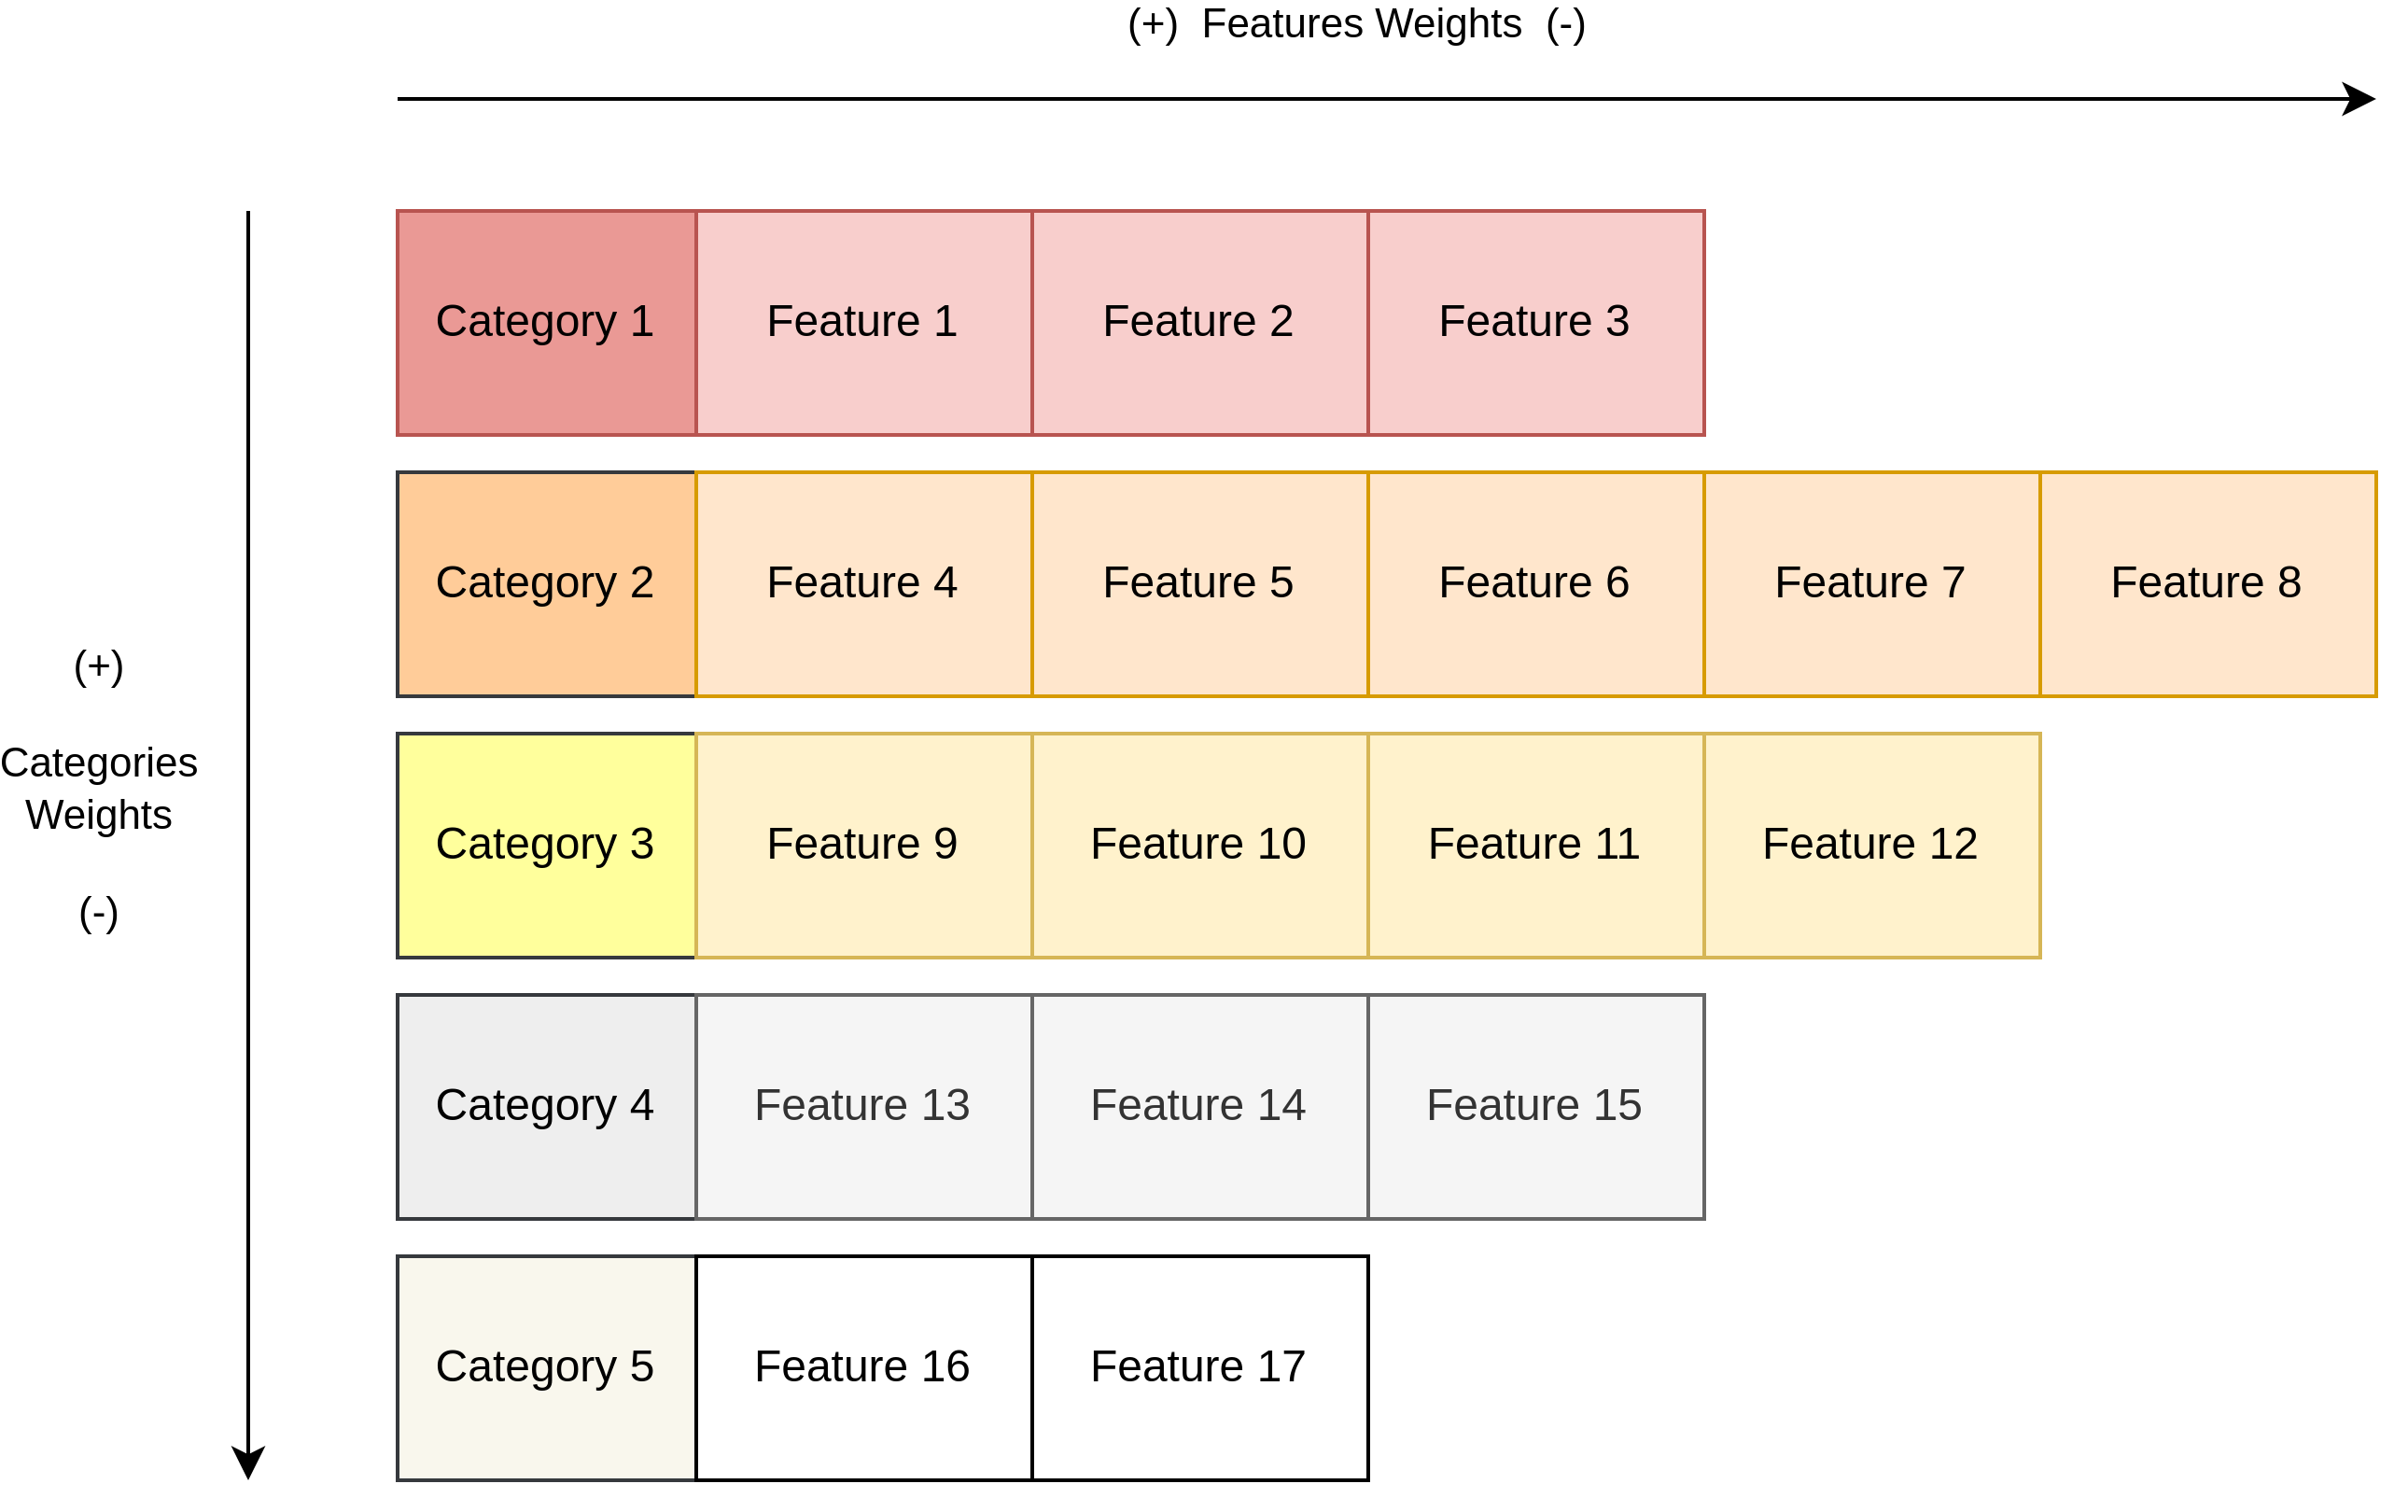
\includegraphics[width=12cm]{Figures/indexing_positions_1_2.png}
	\caption[Asignación de pesos a las categorías en base a las características]{Asignación de pesos a las categorías en base a las características. El peso de las categorías es la suma del peso de las características que la conforman}
	\label{CategoriesFeaturesWeights}
\end{figure}

El resultado de este proceso es una transformación de datos inicialmente tabulares en una matriz $n \times m$, donde $n$ es el número de categorías disponibles en los datos y $m$ es el número de máximo de características que contienen las categorías. Estas matrices están conformadas siguiendo la máxima de que las variables más importantes para los datos se encuentran en las posiciones centrales, como se muestra en la Figura \ref{MatrixIndexes}.


\begin{figure}[H]
	\centering
	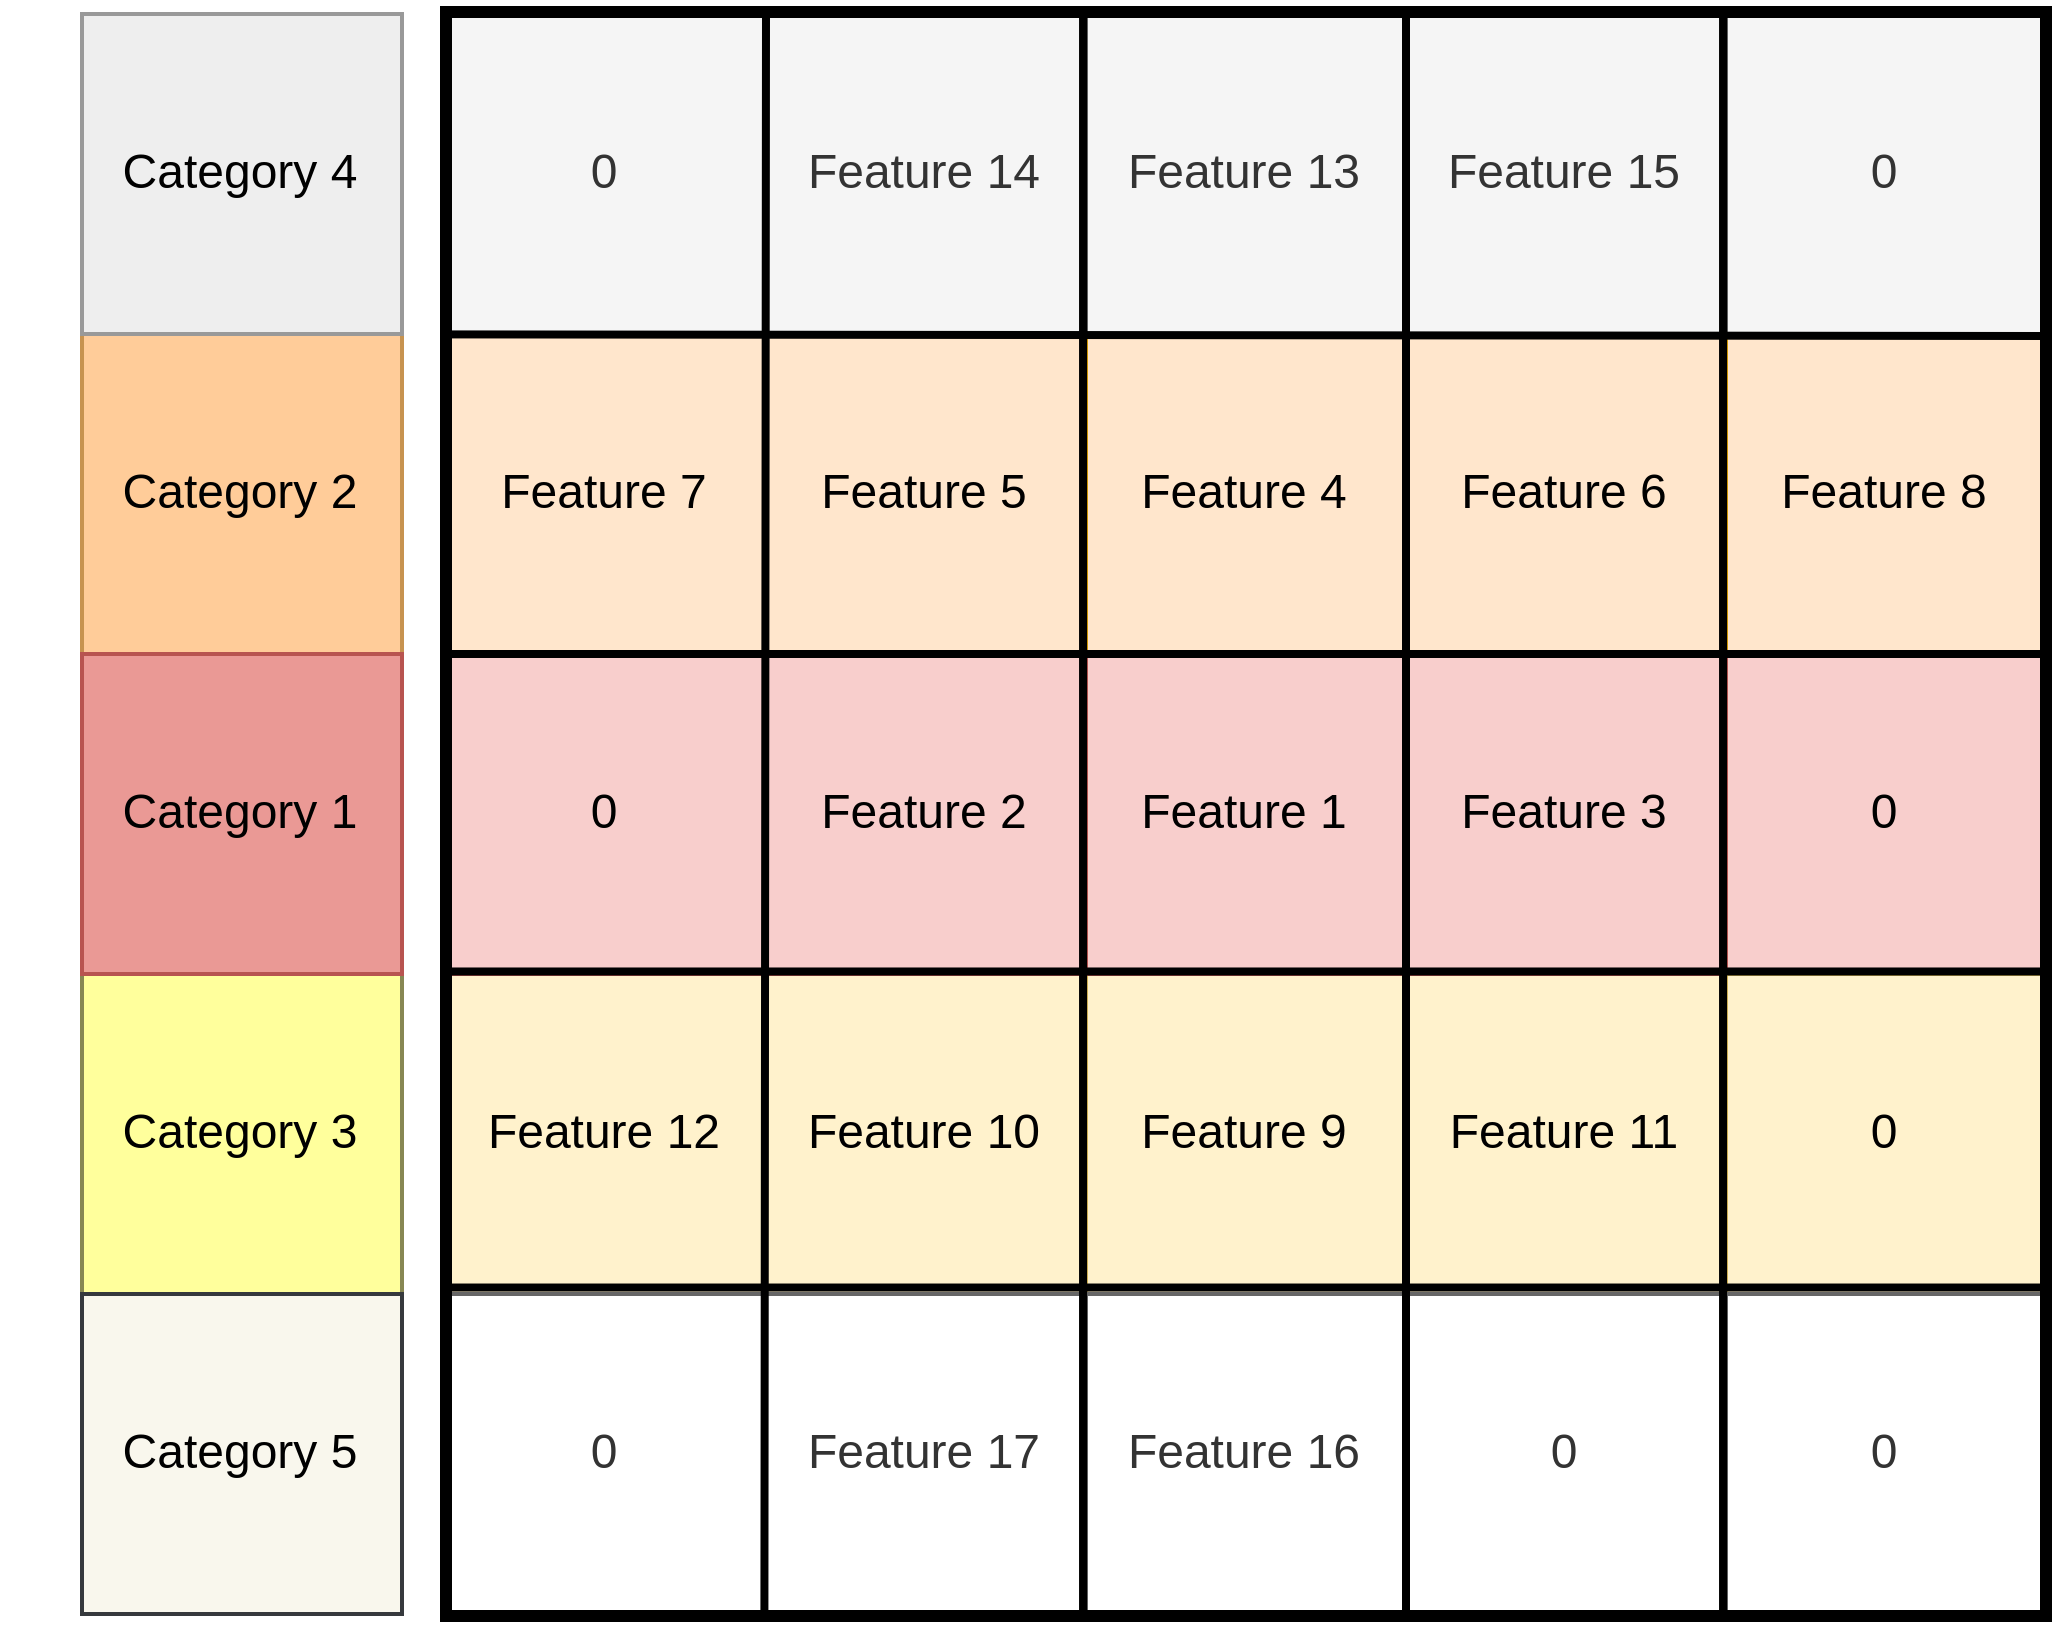
\includegraphics[width=10cm]{Figures/indexing_positions_2.png}
	\caption{Posición de las categorías y características en base a sus pesos}
	\label{MatrixIndexes}
\end{figure}

En la Figura \ref{MatrixConstruction} se muestra un ejemplo de la ejecución de este procedimiento siguiendo el flujo de ejecución del ejemplo de la figura \ref{PostprocessingStage}.

\begin{figure}[H]
	\centering
	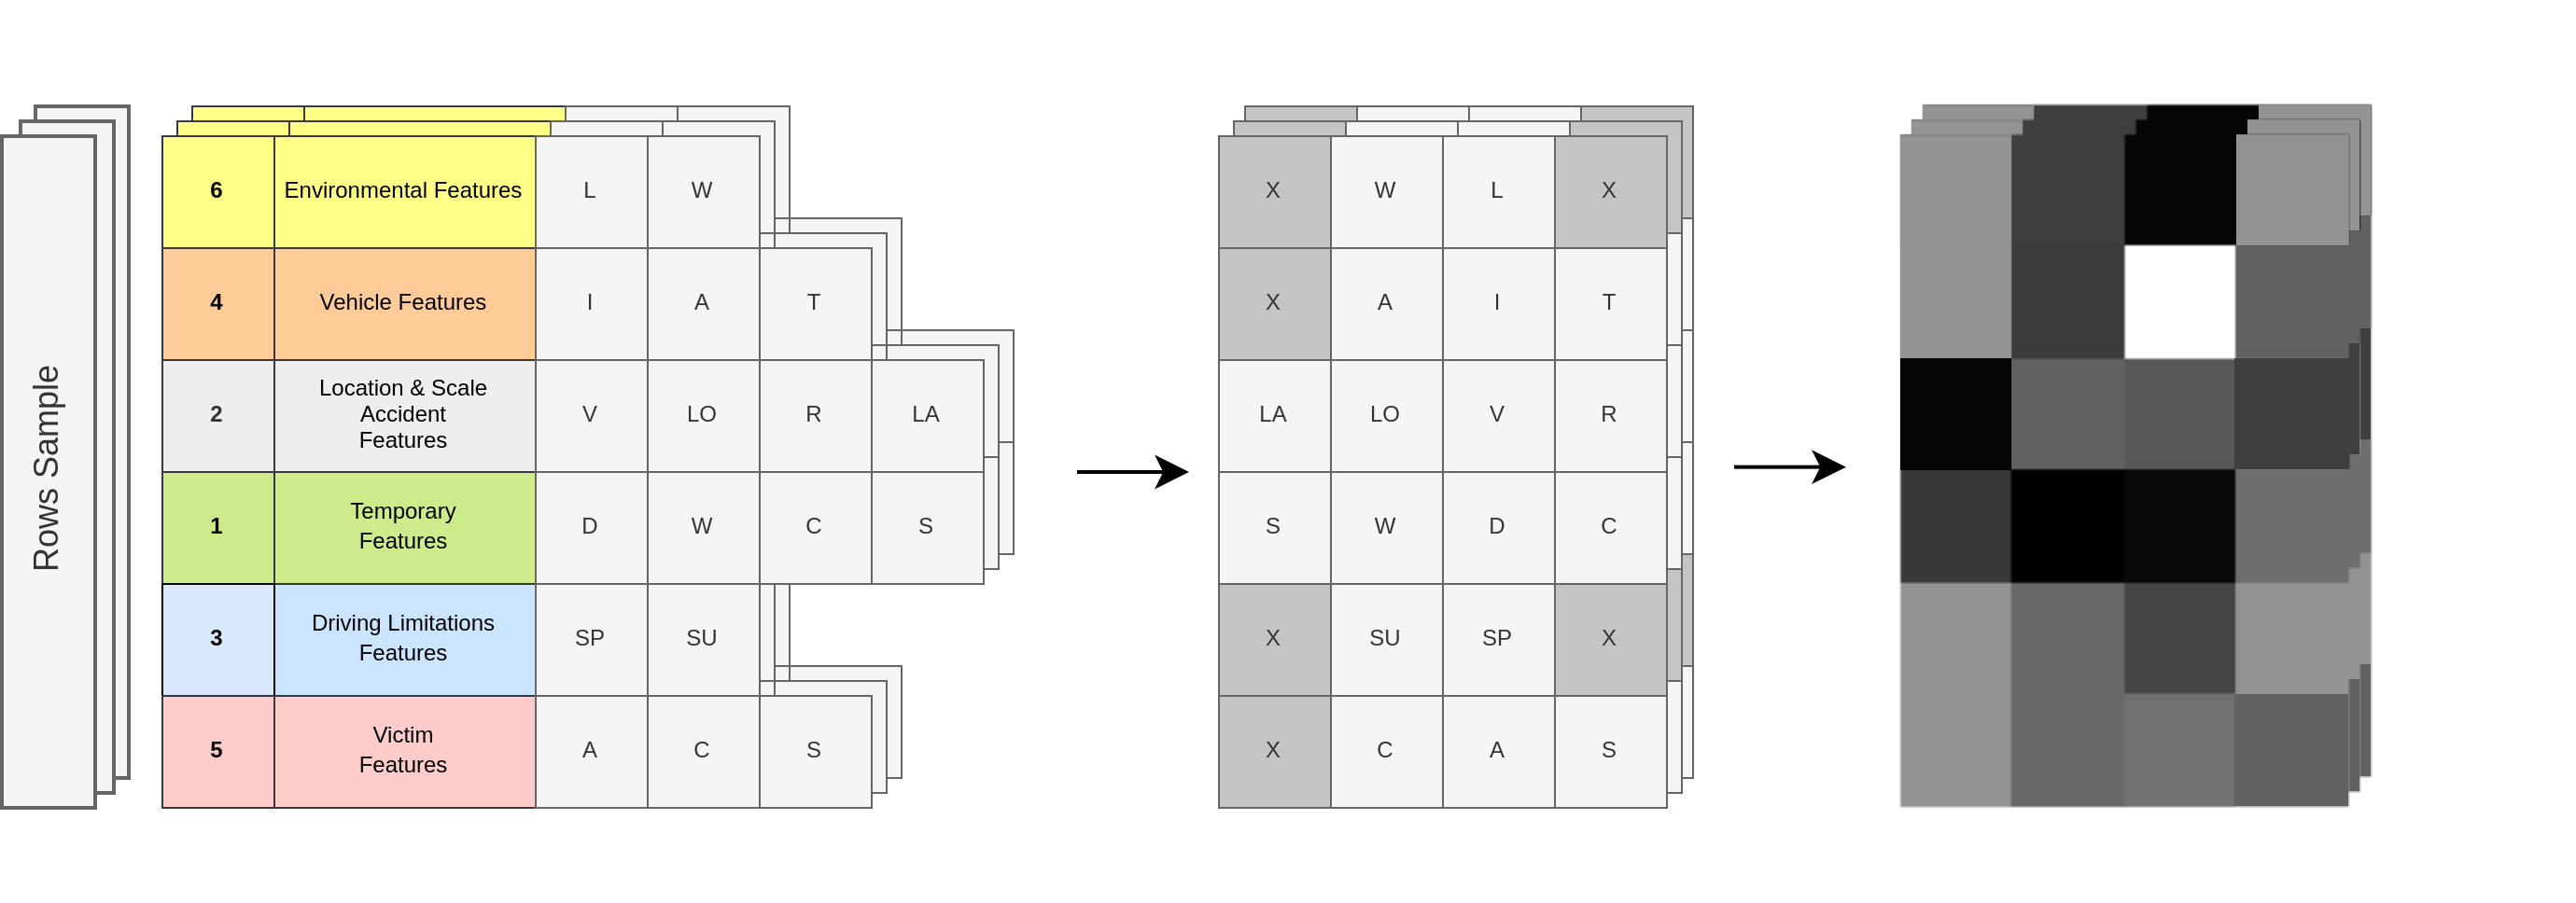
\includegraphics[width=15cm]{Figures/Matrix Construction_2.png}
	\caption[Asignación de características a posiciones de las matrices]{Asignación de características a posiciones de las matrices. Las categorías se asignan a las filas de la matriz en base a su peso; seguidamente, las características de cada categoría se posicionan en las columnas}
	\label{MatrixConstruction}
\end{figure}

\subsubsection{Diseño del modelo}

El nuevo modelo propuesto presenta una arquitectura de cuatro capas convolucionales de dos dimensiones cada una, con un tamaño de \textit{kernel} de $3 \times 3$ y una función de activación \textit{ReLU}. A la salida de cada capa convolucional se aplica un proceso de \textit{Batch Normalization}.

La primera capa convolucional de la red consta de $64$ \textit{kernels}, la segunda de $512$, la tercera de $128$ y la cuarta de $256$. Estos \textit{kernels} contienen los pesos que se entrenan durante la fase de ajuste del modelo a partir de la salida conocida de los datos etiquetados, aprendiendo qué multiplicaciones en los datos minimizan la función de pérdida definida de la red (\textit{Binary Cross Entropy}) gracias al proceso de \textit{Back Propagation}. La salida de cada capa convolucional son los mapas de características (\textit{feature maps}), que son el resultado de aplicar la multiplicación de estos filtros a su entrada. El paso, o número de unidades que avanzan los \textit{kernels}, para un mapa de características, es $1$. También se aplica un relleno en las convoluciones (\textit{padding}), es decir, si la multiplicación del \textit{kernel} excede los límites de la matriz, se agregarán ceros a estos límites para realizar la convolución. Los mapas de características resultantes de la última capa pasan a través de una capa de aplanamiento (\textit{flatten}), que transforma los datos a una sola dimensión una vez que han finalizado las convoluciones. Cada uno de estos datos aplanados está interconectado con los $256$ nodos definidos de la capa densa (\textit{Fully Connected Network}). Finalmente, la capa densa está conectada a una capa final con la función de activación \textit{Softmax}, que da la probabilidad de que cada nueva muestra pertenezca a una de las dos clases. En la figura \ref{CNN2DArchitecture} se puede observar, a modo de diagrama, la arquitectura básica de la red.

\begin{figure}[H]
	\centering
	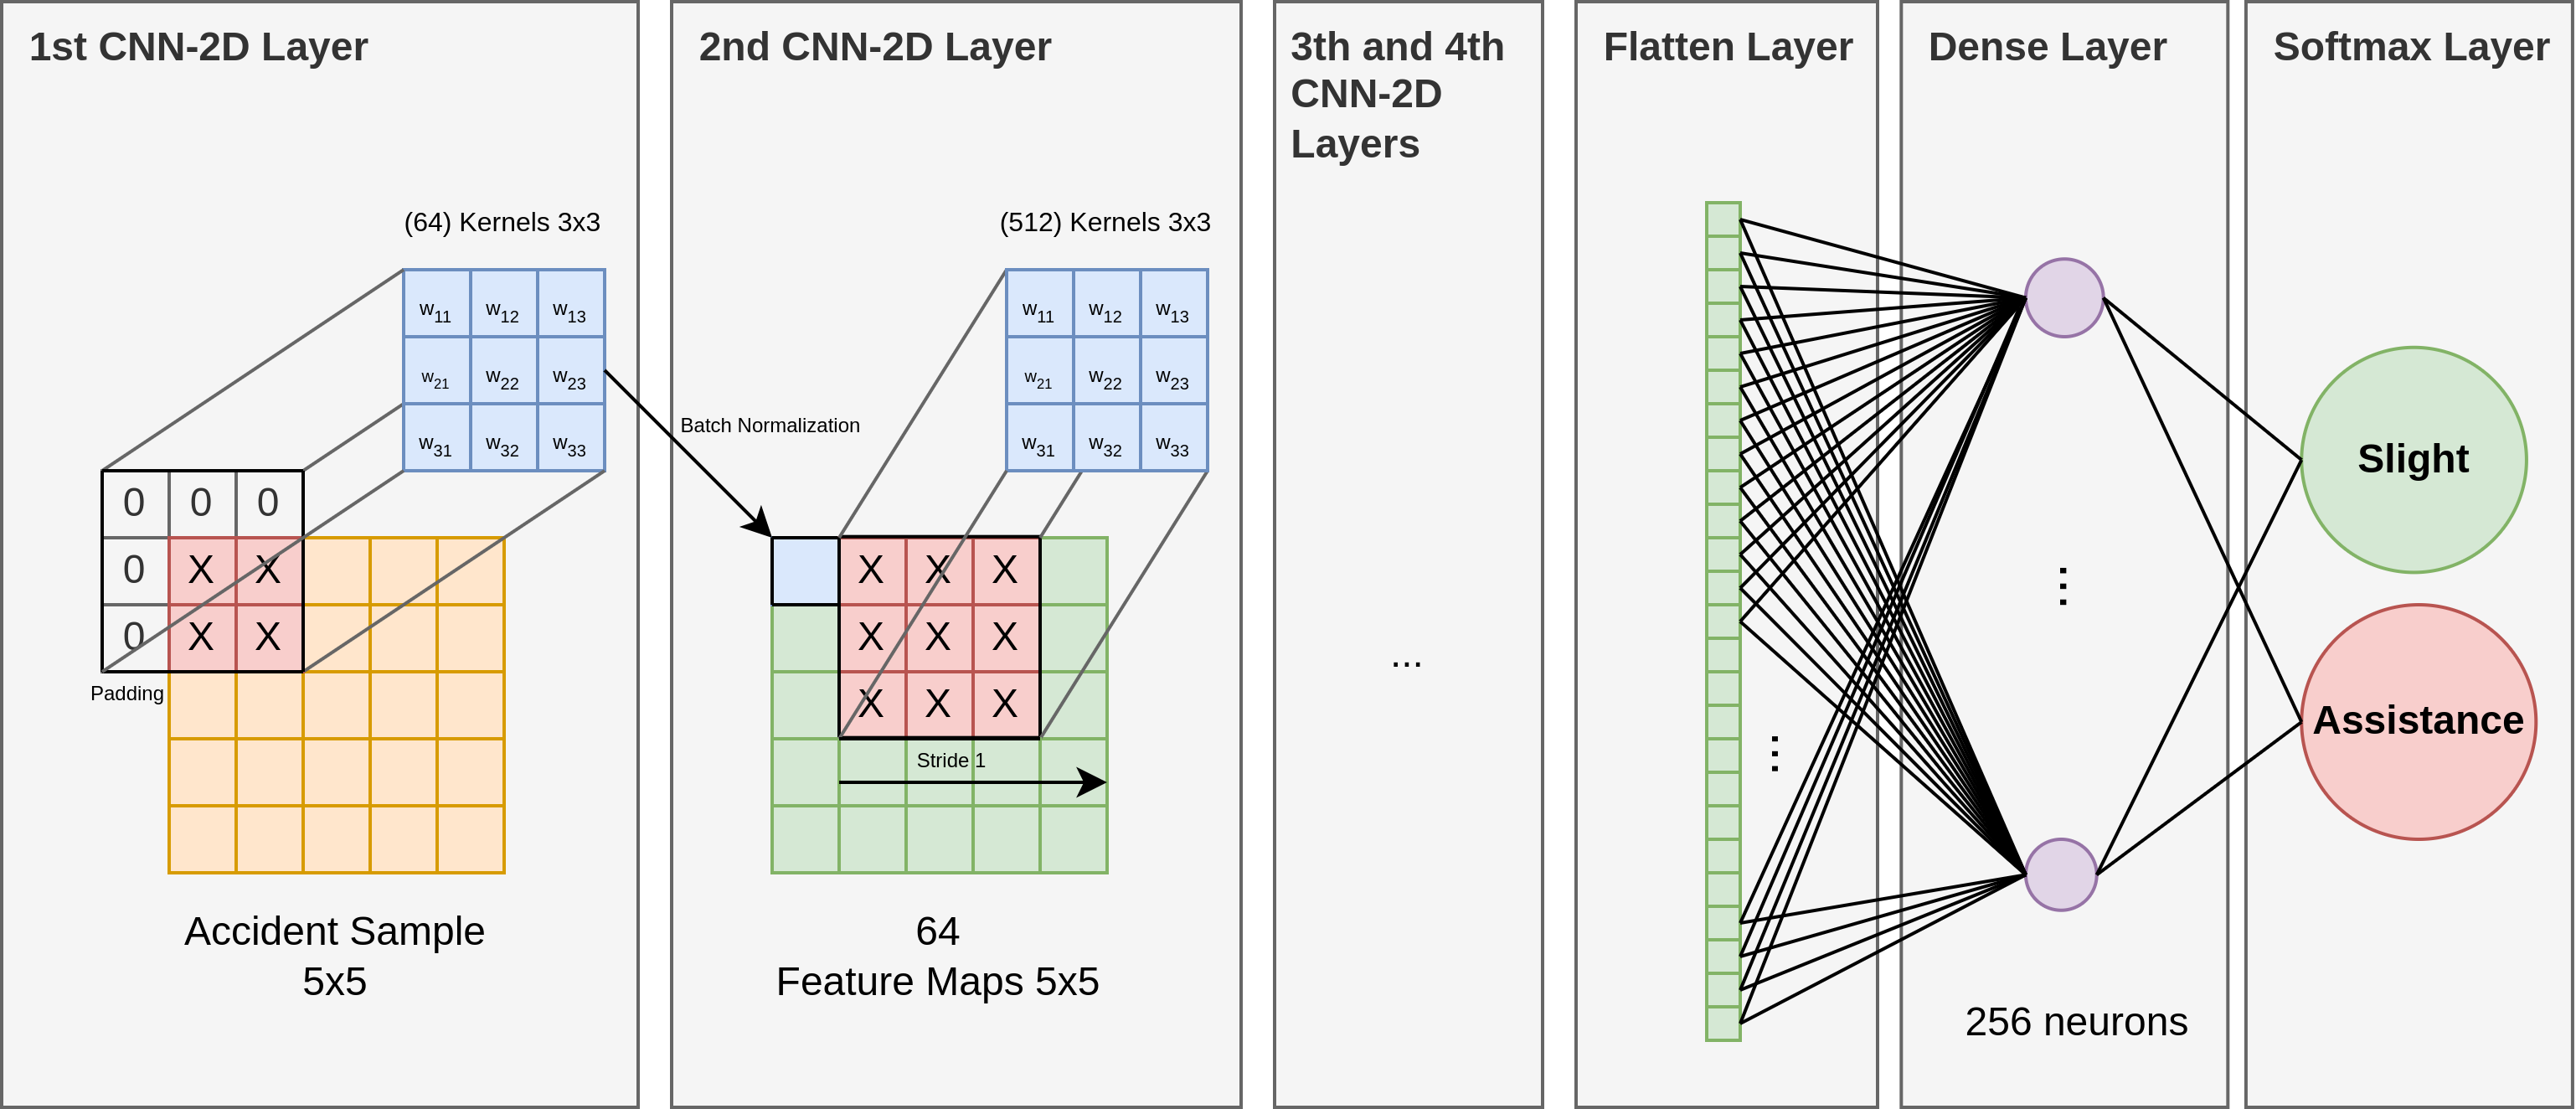
\includegraphics[width=15cm]{Figures/SIMPLE.png}
	\caption{Arquitectura del modelo GTAAF propuesto}
	\label{CNN2DArchitecture}
\end{figure}


\section{Evaluación del modelo: Eficiencia y Robustez}

Para medir el rendimiento y evaluar la capacidad de generalización de la metodología GTAAF, se compararán los resultados ofrecidos por este respecto a otros seis modelos de clasificación del estado del arte (\textit{SVC, Naive Bayes, Random Forest, KNN, Regresión Logística y MLP}) a lo largo de tres datasets de accidentes de tráfico de ocho áreas situadas en distintos lugares del mundo. Concretamente España (Madrid), Reino Unido (Southwark, Manchester, Birmingham, Liverpool, Sheffield y Cornwall), y Australia (estado de Victoria).

Con el objetivo de medir la precisión del modelo en distintos contextos, estas regiones han sido seleccionadas debido a que presentan una alta variabilidad, tanto en los datos que contienen, como la extensión de las regiones y en la densidad de población que presentan. De esta forma es posible evaluar el rendimiento de la metodología distinguiendo entre tres casos de estudio claramente definidos: (1) alta concentración de población, (2) concentración media y (3) concentración dispersa. Con esta variabilidad en los datos se busca medir la robustez y generalización de la técnica desarrollada.

Por otra parte, se han realizado una serie de experimentos ejecutado el modelo GTAAF sobre los conjuntos de datos eliminando características para comprobar la robustez del modelo. En primer lugar, se prescinde aquella que más relevancia tiene para la metodología (mayor peso), en segundo lugar, aquella que menos relevancia tiene (menor peso) y, en un tercer experimento, quitando ambas. Estas pruebas tienen un doble objetivo: evaluar la robustez de la metodología y simular la aplicación del modelo a futuros conjuntos de datos donde no se disponga de valores de todas las características de los conjuntos de datos seleccionados, "eliminando variables significativamente poderosas para los resultados de esta tesis".

Para medir la eficiencia de los modelos se utilizará la métrica \textit{F1-Score}, ya que es una métrica ampliamente utilizada en problemas de clasificación y que representa una buena aproximación a la generalización del modelo, ya que para su cálculo se tienen en cuenta componentes más básicas como la precisión y el recuerdo, indicadores esenciales para una evaluación robusta de cualquier modelo predictivo.
 
      
\chapter{Experimentos y resultados}

En este capítulo se expone la información técnica de interés relativa a los experimentos y resultados realizados en este trabajo. En primer lugar se presentarán los datos sobre los que se han realizado los experimentos. Posteriormente se expondrán los resultados obtenidos por un \textbf{prototipo preliminar} tras su ejecución bajo una población específica, Madrid, que sirve como base para los experimentos relativos al cuarto apartado, donde se presentarán los resultados del modelo final \textbf{GTAAF} aplicado a datos de ocho regiones distintas. La finalidad de esto será validar la generalización del modelo propuesto a través de conjuntos de datos de distintas regiones, concretamente Reino Unido o United Kingdom (UK) para el municipio de Southwark, la ciudad de Manchester, la ciudad de Birmingham, la ciudad de Liverpool, la ciudad de Sheffield y el condado de Cornwall, España (Madrid) y Australia (Estado de Victoria).

% \section{Tecnologías}

% \textcolor{green}{MANU: Tengo dudas de que este apartado vaya aquí o antes. Necesito confirmación. Es que realmente en una tesis doctoral no se si tiene relevancia decir que se ha usado Meets para las reuniones y Diagrams para las figuras, por ejemplo. Creo que son cosas mas de memoria técnica de un TFG/TFM, pero en tesis creo que no...}

% \textcolor{purple}{JOSE: \textbf{opino que no se debe poner}}

% \textcolor{orange}{LUIS: \textbf{pues se quita}}

% En esta sección, se enumeran las herramientas de las que se ha hecho uso durante el trascurso de esta tesis. Como herramienta principal, se ha hecho un uso extensivo de \textit{Python}, un lenguaje de programación de alto nivel y multiparadigma. La versión utilizada para el desarrollo del proyecto fue la 3.9.11 \cite{Python}. Dentro de este lenguaje, las bibliotecas más utilizadas fueron:

% \begin{description}
	%     \item[Pandas:] Ofrece herramientas para el análisis y manipulación de datos. Se usó la versión 1.3.5 \cite{Pandas}.
	
	%     \item[GeoPandas:] Permite la manipulación y análisis de datos que incluyen información espacial, facilitando tareas como la visualización de mapas. La versión utilizada en este trabajo es la 0.12.2 \cite{GeoPandas}.
	
	%     \item[Tensorflow:] Utilizada para implementar redes neuronales y ejecutarlas. Este proyecto se basa en la versión 2.8.0 \cite{Tensorflow}.
	
	%     \item[Sklearn:] Contiene múltiples modelos predictivos implementados, basados en NumPy, SciPy y Matplotlib. La versión configurada para este proyecto es la 1.0.2 \cite{Scikit-Learn}.
	
	%     \item[XGboost:] Implementa el algoritmo XGBoost y ofrece configuraciones para ejecución en \textit{CPU, GPU y GPU paralelizada}. La versión utilizada fue la 1.5.0 \cite{XGBoostLibrary}.
	% \end{description}

% En cuanto a otras herramientas de \textit{software} utilizadas, se destacan las siguientes:

% \begin{description}
	%     \item[CUDA:] Una plataforma de computación paralela que posibilita la ejecución de código en unidades de procesamiento gráfico (\textit{GPU}), lo cual acelera el entrenamiento de redes neuronales en comparación con la unidad central de procesamiento (\textit{CPU}) debido a la rapidez con la que se llevan a cabo las operaciones sobre datos en las tarjetas gráficas. La versión empleada fue la 11.6 \cite{CUDA}.
	
	%     \item[Anaconda:] Una distribución de código abierto que permite mantener múltiples entornos con distintas configuraciones y versiones de diversas bibliotecas, facilitando la migración entre sistemas. La versión utilizada fue la 4.12.0 \cite{Anaconda}.
	
	%     \item[Jupyter Notebook:] Un entorno interactivo que permite la creación, edición y ejecución de cuadernos de manera local o remota. La versión utilizada para este proyecto fue la 6.4.10 \cite{JupyterNotebook}.
	
	%     \item[Jupyter Lab:] Una interfaz de usuario moderna que complementa al entorno Jupyter Notebook y ofrece varias funcionalidades, como la navegación entre diferentes repositorios dentro de la interfaz. La versión utilizada durante el proyecto fue la 3.3.2 \cite{JupyterLab}.
	
	%     \item[DiagramsNet:] Una plataforma empleada para la elaboración de figuras mostradas en este documento \cite{DiagramsNet}.
	
	%     \item[Google Meets:] Una plataforma utilizada para llevar a cabo reuniones mensuales con los tutores \cite{GoogleMeet}.
	% \end{description}


%     Como sistema de control de versiones se ha utilizado \textit{Github} \cite{Github}, repositorio donde es posible subir versiones del proyecto.


% Los experimentos de esta tesis se han dividido en varios entornos. El primero de ellos, utilizado para el entrenamiento del primer prototipo, se trataba de un servidor con CPU \textit{Dual AMD Rome 7742} (128 cores) y contando con una GPU \textit{DGX NVIDIA A100} de  40 GigaBytes (\textit{GB}). Para el entrenamiento del modelo definitivo propuesto se hizo uso de una máquina con un procesador Intel Core i7-12700F, con 64 GB de RAM VENGEANCE LPX (2 x 32GB) DDR4 DRAM a 3200MHz y una tarjeta gráfica NVIDIA GeForce RTX 3090 Ti.




\section{Adaptación de los datos}
\label{DATA_PRESENTATION_RESULTS}

% \textcolor{red}{Luis: Este párrafo está regular. Por otra parte colapsa con el apartado Evaluación del modelo: Eficiencia y Robustez. Aunque no sé si está mal que sea así..}
% \textcolor{purple}{JOSE: \textbf{ahora lo veo bien}}

En este punto se presentan los datos sobre los que se han trabajado en esta tesis. Los datos escogidos para la validación pertenecen a tres regiones diferentes, donde cada una de ellas presenta distintas singularidades. El criterio escogido para la selección de estos datos se basa en la búsqueda de la variabilidad a lo largo de distintos contextos y casos de uso con el objetivo de validar que el modelo propuesto es capaz de generalizar a través de múltiples circunstancias. Esta evaluación se basará en dos factores principales: (1) la distinta disponibilidad de información en los conjuntos de datos y (2) en función de la densidad de población de las regiones escogidas. A su vez, para este último factor de la densidad de población, distinguiremos tres casos de estudio claramente diferenciados: alta concentración de población, concentración media y concentración dispersa. Con esta variabilidad en los datos se busca medir la robustez y generalización del modelo GTAAF desarrollado.



\subsection*{Madrid}

El primer conjunto de datos seleccionado para su adaptación contiene información de accidentes de tráfico sobre la Comunidad de Madrid, comprendidos entre los años $2019$ y $2022$ a lo largo de toda la ciudad. Estos datos describen los accidentes mediante 18 características para $73\,514$ registros totales, extraídos desde el Portal de Datos Abiertos del Ayuntamiento de Madrid \cite{InfoDatasetMadrid}. 

La alta densidad de población de Madrid convierte a este conjunto de datos en un caso de estudio de alta concentración de población, en la Tabla \ref{Madrid_statistics} se pueden observar los datos de geográficos y de accidentes sobre esta ciudad.

\begin{table}[ht]
	\caption[Descripción de las propiedades geográficas de acuerdo a los accidentes de Madrid]{Descripción de las propiedades geográficas de acuerdo a los accidentes de Madrid. El \textit{Ratio de accidentes} representa el número de accidentados por año}
	\begin{center}
		\begin{tabular}{|c|c||c|c|c|c|c|c|}
			\hline
			\textbf{Dataset} & \textbf{$Km^2$} & \textbf{Habitantes} & \textbf{Habitantes por $km^2$} & \textbf{Ratio de accidentes}
			\\ \hline \hline
			
			Madrid & 604,3 & 3.339.931 & 5.530 & 0,0055 \\ \hline
			
		\end{tabular}
	\end{center}
	\label{Madrid_statistics}
\end{table}

Las características originales presentes en este conjunto de datos se encuentran descritas en la Tabla \ref{Datadescription}:

%%%%%%%%%%%%%%%%%%%%%%%%%%%%%%%%%%%%%%%%%%%%%%%%%%%%%%%%%%%%%%%%%%%%%%%%%%%%%%%%%
\begin{table}[ht]
	\caption{Variables del conjunto de datos de Madrid y sus descripciones}
	\begin{center}
		\begin{tabular}{|p{3cm}|p{10cm}|}
			\hline
			\textbf{Atributo} & \textbf{Descripción} \\ \hline \hline
			ID de Incidente  & Identificador del incidente, si varios registros tienen el mismo número de archivo, se consideran el mismo accidente y cada registro representa a cada una de las personas involucradas en él (conductor, pasajero o peatón)  \\ \hline
			Fecha  & Día/mes/año del accidente \\ \hline
			Hora  & Hora exacta en la que ocurrió el accidente \\ \hline
			Tipo de Carretera & Tipo de carretera donde ocurrió el incidente \\ \hline
			Nombre & Nombre de la calle donde ocurrió el incidente \\ \hline
			Número de Calle & Número de la calle donde ocurrió el incidente  \\ \hline
			Distrito & Nombre del distrito donde ocurrió el incidente \\ \hline
			Tipo de Accidente  & Puede ser: doble colisión, colisión múltiple, alcance, colisión con un obstáculo, atropello, vuelco, caída u otras causas \\ \hline
			Clima  & Condiciones climáticas en el momento del incidente \\ \hline
			Vehículo  & Clasificación según tipos de vehículos \\ \hline
			Persona  & Rol de la persona involucrada: conductor, pasajero o peatón \\ \hline
			Edad  & Rango de edad de la persona involucrada \\ \hline
			Género  & Mujer u hombre \\ \hline
			Gravedad & Consecuencias físicas de la persona involucrada, si han necesitado atención médica, si han sido hospitalizados o si han sido fatales \\ \hline
			X   & Coordenada X - UTM \\ \hline
			Y   & Coordenada Y - UTM \\ \hline
			Alcohol & Si la persona involucrada ha dado positivo en alcohol (S o N) \\ \hline
			Drogas & Si la persona involucrada ha dado positivo en drogas (S o N) \\ \hline \hline
		\end{tabular}
	\end{center}

	\label{Datadescription}
\end{table}
%%%%%%%%%%%%%%%%%%%%%%%%%%%%%%%%%%%%%%%%%%%%%%%%%%%%%%%%%%%%%%%%%%%%%%%%%%%%%%%%%

En lo que respecta a la variable a predecir, la \textbf{Gravedad} del accidente, en este conjunto de datos se presentan distintos valores que puede tomar. A continuación se presentan las descripciones que puede tomar esta característica junto con su valor numérico original:

\begin{itemize}
	\item Atención de emergencia sin posterior admisión hospitalaria: $1$.
	\item Admisión hospitalaria menor o igual a 24 horas: $2$.
	\item Hospitalización por más de $24$ horas: $3$.
	\item Fallecido dentro de las $24$ horas: $4$.
	\item Atención médica ambulatoria después del accidente: $5$.
	\item Atención médica solo en el lugar del accidente: $6$.
	\item Sin atención médica: $7$.
\end{itemize}

Hay que resaltar que el conjunto de datos de la ciudad de Madrid se utilizará para validar ambos modelos (preliminar y GTAAF). Por este motivo, la interpretación de los valores que toma la variable de la gravedad del accidente serán considerados de forma distinta en cada una de ellas. En el modelo preliminar se interpretará como tres posibles clases (\textbf{leves}, \textbf{severos} y \textbf{fatales}), y  en el modelo GTAAF se considerará como dos (\textbf{con necesidad de asistencia} y \textbf{sin necesidad de asistencia}).


\subsection*{Victoria}

El segundo caso de estudio contempla una situación de concentración de población dispersa, concretamente a lo largo del Estado de Victoria, Australia. Este conjunto de datos contempla accidentes producidos entre el año $2000$ y el $2005$, contando con un total de $14\,123$ registros. Este conjunto de datos ha sido obtenido a través del Departamento de Transportes y Planificación del Gobierno del estado de Victoria \cite{InfoDatasetVictoria}.

Como se puede apreciar en la tabla \ref{Victoria_statistics}, el caso de uso aplicado del estado de Victoria se muestra como una situación de baja concentración de población. Al ser un estado muy extenso, las densidades de población se encuentran en los núcleos urbanos, siendo el número de habitantes por kilómetro cuadrado considerablemente bajo en comparación con el resto de datos estudiados en esta tesis.

\begin{table}[H]
	\caption[Descripción de las propiedades geográficas de acuerdo a los accidentes de Victoria]{Descripción de las propiedades geográficas de acuerdo a los accidentes de Victoria. El \textit{Ratio de accidentes} representa el número de accidentados por año}
	\begin{center}
		\begin{tabular}{|c|c||c|c|c|c|c|c|}
			\hline
			\textbf{Dataset} & \textbf{$Km^2$} & \textbf{Habitantes} & \textbf{Habitantes por $km^2$} & \textbf{Ratio de accidentes}
			\\ \hline \hline
			Victoria & 227.416 &  5.603.100  & 25  & 0,0004\\ \hline
		\end{tabular}
	\end{center}

	\label{Victoria_statistics}
\end{table}


En este caso, se disponen de $140$ características divididas en varias bases de datos sobre las que se han realizado operaciones de unión para disponer de los datos en su totalidad. Gran parte de estas características contemplan información que no aporta valor descriptivo para los accidentes, ya que se tratan de definiciones de los valores numéricos asignados en otras columnas, identificadores para hacer uniones entre las tablas, entre otros. Estas tablas contienen información relativa a:

\begin{itemize}
	\item \textbf{Víctimas del accidente} \ref{Victoria_CASUALTY_TABLE}
	\item \textbf{Descriptores del accidente} \ref{Victoria_ACCIDENT_TABLE}
	\item \textbf{Características de la carretera} \ref{Victoria_ROAD_SURF_TABLE}
	\item \textbf{Condiciones atmosféricas} \ref{Victoria_ATMOS_COND_TABLE}
	\item \textbf{Vehículos implicados} \ref{Victoria_VEHICLE_TABLE}
	\item \textbf{Evento del accidente} \ref{Victoria_ACCIDENT_EVENT_TABLE}
	\item \textbf{Localización del accidente} \ref{Victoria_ACCIDENT_LOCATION_TABLE}
	\item \textbf{Características del nodo} \ref{Victoria_NODE_TABLE}
\end{itemize}

A continuación se describirán los datos contemplados en cada una de estas tablas.

\begin{table}[H]
	\caption{Descripción de características de la tabla Víctima de los datos de Victoria}
	\begin{center}
		\begin{tabular}{|c|l|}
			\hline
			\multicolumn{2}{ |c| }{\textbf{Tabla Víctima}} \\ \hline
			\textbf{Atributo} & \textbf{Descripción} \\ \hline
			\hline
			ACCIDENT\_NO & Número de accidente \\ \hline
			PERSON\_ID & ID de la persona \\ \hline
			VEHICLE\_ID & ID del vehículo \\ \hline
			SEX & Género \\ \hline
			AGE & Edad \\ \hline
			AGE\_GROUP & Grupo de edad \\ \hline
			\textbf{INJ\_LEVEL} & \textbf{Nivel de lesión} \\ \hline
			INJ\_LEVEL\_DESC & Descripción del nivel de lesión \\ \hline
			SEATING\_POSITION & Posición en el asiento \\ \hline
			HELMET\_BELT\_WORN & Uso de casco o cinturón de seguridad \\ \hline
			ROAD\_USER\_TYPE & Tipo de usuario de la carretera \\ \hline
			ROAD\_USER\_TYPE\_DESC & Descripción del tipo de usuario de la carretera \\ \hline
			LICENCE\_STATE & Estado de la licencia \\ \hline
			PEDEST\_MOVEMENT & Movimiento del peatón \\ \hline
			POSTCODE & Código postal \\ \hline
			TAKEN\_HOSPITAL & Hospital al que fue llevado \\ \hline
			EJECTED\_CODE & Código de expulsión \\ \hline
		\end{tabular}
	\end{center}

	\label{Victoria_CASUALTY_TABLE}
\end{table} 

\begin{table}[H]
	\caption{Descripción de características de la tabla Accidente de los datos de Victoria}
	\begin{center}
		\begin{tabular}{|c|l|}
			\hline
			\multicolumn{2}{ |c| }{\textbf{Tabla Accidente}} \\ \hline
			\textbf{Atributo} & \textbf{Descripción} \\ \hline
			\hline
			ACCIDENT\_NO & Número de accidente \\ \hline
			ACCIDENT\_DATE & Fecha del accidente \\ \hline
			ACCIDENT\_TIME & Hora del accidente \\ \hline
			ACCIDENT\_TYPE & Tipo de accidente \\ \hline
			ACCIDENT\_TYPE\_DESC & Descripción del tipo de accidente \\ \hline
			DAY\_OF\_WEEK & Día de la semana \\ \hline
			DAY\_OF\_WEEK\_DESC & Descripción del día de la semana \\ \hline
			DCA\_CODE & Código DCA \\ \hline
			DCA\_DESCRIPTION & Descripción DCA \\ \hline
			DIRECTORY & Directorio \\ \hline
			EDITION & Edición \\ \hline
			PAGE & Página \\ \hline
			GRID\_REFERENCE\_X & Referencia de cuadrícula (X) \\ \hline
			GRID\_REFERENCE\_Y & Referencia de cuadrícula (Y) \\ \hline
			LIGHT\_CONDITION & Condición de luz \\ \hline
			LIGHT\_CONDITION\_DESC & Descripción de la condición de luz \\ \hline
			NODE\_ID & ID de nodo \\ \hline
			NO\_OF\_VEHICLES & Número de vehículos \\ \hline
			NO\_PERSONS & Número de personas \\ \hline
			NO\_PERSONS\_INJ\_2 & Número de personas heridas levemente \\ \hline
			NO\_PERSONS\_INJ\_3 & Número de personas heridas gravemente \\ \hline
			NO\_PERSONS\_KILLED & Número de personas fallecidas \\ \hline
			NO\_PERSONS\_NOT\_INJ & Número de personas no heridas \\ \hline
			POLICE\_ATTEND & Asistencia policial presente \\ \hline
			ROAD\_GEOMETRY & Geometría de la carretera \\ \hline
			ROAD\_GEOMETRY\_DESC & Descripción de la geometría de la carretera \\ \hline
			SEVERITY & Gravedad del accidente \\ \hline
			SPEED\_ZONE & Zona de velocidad \\ \hline
		\end{tabular}
	\end{center}

	\label{Victoria_ACCIDENT_TABLE}
\end{table} 


\begin{table}[H]
	\caption{Descripción de características de la tabla Características de la Carretera de los datos de Victoria}
	\begin{center}
		\begin{tabular}{|c|l|}
			\hline
			\multicolumn{2}{ |c| }{\textbf{Tabla Características de Carretera}} \\ \hline
			\textbf{Atributo} & \textbf{Descripción} \\ \hline
			\hline
			ACCIDENT\_NO & Número de accidente \\ \hline
			SURFACE\_COND & Condición de la superficie \\ \hline
			SURFACE\_COND\_DESC & Descripción de la condición de la superficie \\ \hline
			SURFACE\_COND\_SEQ & Secuencia de la condición de la superficie \\ \hline
		\end{tabular}
	\end{center}

	\label{Victoria_ROAD_SURF_TABLE}
\end{table} 


\begin{table}[H]
	\caption{Descripción de características de la tabla Características Atmosféricas de los datos de Victoria}
	\begin{center}
		\begin{tabular}{|c|l|}
			\hline
			\multicolumn{2}{ |c| }{\textbf{Tabla Características Atmosféricas}} \\ \hline
			\textbf{Atributo} & \textbf{Descripción} \\ \hline
			\hline
			ACCIDENT\_NO & Número de accidente \\ \hline
			ATMOSPH\_COND & Condición atmosférica \\ \hline
			ATMOSPH\_COND\_SEQ & Secuencia de la condición atmosférica \\ \hline
			ATMOSPH\_COND\_DESC & Descripción de la condición atmosférica \\ \hline
		\end{tabular}
	\end{center}

	\label{Victoria_ATMOS_COND_TABLE}
\end{table} 

\begin{table}[H]
	\caption{Descripción de características de la tabla Vehículo de los datos de Victoria}
	\begin{center}
		\begin{tabular}{|c|l|}
			\hline
			\multicolumn{2}{ |c| }{\textbf{Tabla Vehículo}} \\ \hline
			\textbf{Atributo} & \textbf{Descripción} \\ \hline
			\hline
			ACCIDENT\_NO & Número de accidente \\ \hline
			VEHICLE\_ID & ID del vehículo \\ \hline
			VEHICLE\_YEAR\_MANUF & Año de fabricación del vehículo \\ \hline
			VEHICLE\_DCA\_CODE & Código DCA del vehículo \\ \hline
			INITIAL\_DIRECTION & Dirección inicial \\ \hline
			ROAD\_SURFACE\_TYPE & Tipo de superficie de la carretera \\ \hline
			ROAD\_SURFACE\_DESC & Descripción del tipo de superficie de la carretera \\ \hline
			REG\_STATE & Estado de registro \\ \hline
			VEHICLE\_BODY\_STYLE & Estilo del cuerpo del vehículo \\ \hline
			VEHICLE\_MAKE & Marca del vehículo \\ \hline
			VEHICLE\_MODEL & Modelo del vehículo \\ \hline
			VEHICLE\_POWER & Potencia del vehículo \\ \hline
			VEHICLE\_TYPE & Tipo de vehículo \\ \hline
			VEHICLE\_TYPE\_DESC & Descripción del tipo de vehículo \\ \hline
			VEHICLE\_WEIGHT & Peso del vehículo \\ \hline
			CONSTRUCTION\_TYPE & Tipo de construcción \\ \hline
			FUEL\_TYPE & Tipo de combustible \\ \hline
			NO\_OF\_WHEELS & Número de ruedas \\ \hline
			NO\_OF\_CYLINDERS & Número de cilindros \\ \hline
			SEATING\_CAPACITY & Capacidad de asientos \\ \hline
			TARE\_WEIGHT & Peso tara \\ \hline
			TOTAL\_NO\_OCCUPANTS & Número total de ocupantes \\ \hline
			CARRY\_CAPACITY & Capacidad de carga \\ \hline
			CUBIC\_CAPACITY & Capacidad cúbica \\ \hline
			FINAL\_DIRECTION & Dirección final \\ \hline
			DRIVER\_INTENT & Intención del conductor \\ \hline
			VEHICLE\_MOVEMENT & Movimiento del vehículo \\ \hline
			TRAILER\_TYPE & Tipo de remolque \\ \hline
			VEHICLE\_COLOUR\_1 & Color del vehículo 1 \\ \hline
			VEHICLE\_COLOUR\_2 & Color del vehículo 2 \\ \hline
			CAUGHT\_FIRE & Incendio del vehículo \\ \hline
			INITIAL\_IMPACT & Impacto inicial \\ \hline
			LAMPS & Lámparas \\ \hline
			LEVEL\_OF\_DAMAGE & Nivel de daño \\ \hline
			OWNER\_POSTCODE & Código postal del propietario \\ \hline
			TOWED\_AWAY\_FLAG & Indicador de remolque \\ \hline
			TRAFFIC\_CONTROL & Control de tráfico \\ \hline
			TRAFFIC\_CONTROL\_DESC & Descripción del control de tráfico \\ \hline
		\end{tabular}
	\end{center}

	\label{Victoria_VEHICLE_TABLE}
\end{table} 

\begin{table}[H]
	\caption{Descripción de características de la tabla Evento-Accidente de los datos de Victoria}
	\begin{center}
		\begin{tabular}{|c|l|}
			\hline
			\multicolumn{2}{ |c| }{\textbf{Tabla Evento Accidente}} \\ \hline
			\textbf{Atributo} & \textbf{Descripción} \\ \hline
			\hline
			ACCIDENT\_NO & Número de accidente \\ \hline
			EVENT\_SEQ\_NO & Número de secuencia del evento \\ \hline
			EVENT\_TYPE & Tipo de evento \\ \hline
			EVENT\_TYPE\_DESC & Descripción del tipo de evento \\ \hline
			VEHICLE\_1\_ID & ID del vehículo 1 \\ \hline
			VEHICLE\_1\_COLL\_PT & Punto de colisión del vehículo 1 \\ \hline
			VEHICLE\_1\_COLL\_PT\_DESC & Descripción del punto de colisión del vehículo 1 \\ \hline
			VEHICLE\_2\_ID & ID del vehículo 2 \\ \hline
			VEHICLE\_2\_COLL\_PT & Punto de colisión del vehículo 2 \\ \hline
			VEHICLE\_2\_COLL\_PT\_DESC & Descripción del punto de colisión del vehículo 2 \\ \hline
			PERSON\_ID & ID de la persona \\ \hline
			OBJECT\_TYPE & Tipo de objeto \\ \hline
			OBJECT\_TYPE\_DESC & Descripción del tipo de objeto \\ \hline
		\end{tabular}
	\end{center}

	\label{Victoria_ACCIDENT_EVENT_TABLE}
\end{table} 

\begin{table}[H]
	\caption{Descripción de características de la tabla Localización de Accidente de los datos de Victoria}
	\begin{center}
		\begin{tabular}{|c|l|}
			\hline
			\multicolumn{2}{ |c| }{\textbf{Tabla Localización de Accidente}} \\ \hline
			\textbf{Atributo} & \textbf{Descripción} \\ \hline
			\hline
			ACCIDENT\_NO & Número de accidente \\ \hline
			NODE\_ID & ID del nodo \\ \hline
			ROAD\_ROUTE\_1 & Ruta de la carretera 1 \\ \hline
			ROAD\_NAME & Nombre de la carretera \\ \hline
			ROAD\_TYPE & Tipo de carretera \\ \hline
			ROAD\_NAME\_INT & Nombre de la carretera (intersección) \\ \hline
			ROAD\_TYPE\_INT & Tipo de carretera (intersección) \\ \hline
			DISTANCE\_LOCATION & Distancia de la ubicación \\ \hline
			DIRECTION\_LOCATION & Dirección de la ubicación \\ \hline
			NEAREST\_KM\_POST & Kilómetro de poste más cercano \\ \hline
			OFF\_ROAD\_LOCATION & Ubicación fuera de la carretera \\ \hline
		\end{tabular}
	\end{center}

	\label{Victoria_ACCIDENT_LOCATION_TABLE}
\end{table} 


\begin{table}[H]
	\caption{Descripción de características de la tabla Nodo de los datos de Victoria}
	\begin{center}
		\begin{tabular}{|c|l|}
			\hline
			\multicolumn{2}{ |c| }{\textbf{Tabla Nodo}} \\ \hline
			\textbf{Atributo} & \textbf{Descripción} \\ \hline
			\hline
			ACCIDENT\_NO & Número de accidente \\ \hline
			NODE\_ID & ID del nodo \\ \hline
			NODE\_TYPE & Tipo de nodo \\ \hline
			AMG\_X & Coordenada AMG-X \\ \hline
			AMG\_Y & Coordenada AMG-Y \\ \hline
			LGA\_NAME & Nombre del área del gobierno local (LGA) \\ \hline
			REGION\_NAME & Nombre de la región \\ \hline
			DEG\_URBAN\_NAME & Nombre del área urbana \\ \hline
			LAT & Latitud \\ \hline
			LONG & Longitud \\ \hline
			POSTCODE\_N0 & Código postal \\ \hline
		\end{tabular}
	\end{center}

	\label{Victoria_NODE_TABLE}
\end{table} 

% \textcolor{red}{\textbf{Luis, inquietud:} He visto la documentación de los datos, esta es la única información que hay, no describen qué casos exactos van a cada una de las clases...}
% \textcolor{green}{MANU: no puedes inventarte cosas. Si en la documentacion es lo que hay, no hay mas vuelta de tuerca...}
% \textcolor{purple}{JOSE: \textbf{inquietud resuleta}}

En lo que respecta a la variable predictiva que indica la gravedad de las víctimas en los accidentes, este conjunto de datos categoriza las lesiones en cuatro clases:

\begin{enumerate}
	\item Fatales
	\item Graves
	\item Otro tipo de lesiones
	\item Sin lesiones
\end{enumerate}


\subsection*{Reino Unido}

El tercer conjunto de datos pertenece al Departamento de Transportes de Reino Unido \cite{DatasetUK}, donde se contempla información de los accidentes producidos entre el año $2005$ y $2020$ a lo largo de todo el país. Sobre este conjunto de datos se han seleccionado 6 regiones diferentes: Southwark, Manchester, Birmingham, Liverpool, Sheffield y Cornwall. Cada una de ellas presenta un caso de uso distinto en función de su densidad de población. 

Estos datos disponen, en su versión original, de $77$ características que describen información acerca de los accidentes, las víctimas y los vehículos implicados en ellos en bases de datos separadas. Por lo que para obtener la información total desglosada por víctima se realizan operaciones de unión entre ellas. En la tabla \ref{UK_DATASET_SAMPLES_NUMBERS} se puede observar la cantidad de registros resultantes tras realizar estas operaciones en cada una de las regiones seleccionadas.

%%%%%%%%%%%%%%%%%%%%%%%%%%%%%%%%%%%%%%%%%%%%%%%%%%%%%%%%%%%%%%%%%%%%%%%%%%%%%%%%%
\begin{table}[h!]
	\caption{Número original de muestras de las regiones del Reino Unido}
	\centering
	\begin{tabular}{|c|c|}
		\hline
		\multicolumn{2}{ |c| }{\textbf{Distribución de datos de Reino Unido}} \\ \hline
		\textbf{Región} & \textbf{Número de muestras} \\ \hline
		\hline
		Southwark  & 30.214 \\ \hline
		Manchester & 53.341 \\ \hline
		Birmingham & 119.910 \\ \hline
		Liverpool  & 54.452 \\ \hline
		Sheffield  & 49.466 \\ \hline
		Cornwall   & 37.846 \\ \hline \hline
	\end{tabular}

	\label{UK_DATASET_SAMPLES_NUMBERS}
\end{table}
%%%%%%%%%%%%%%%%%%%%%%%%%%%%%%%%%%%%%%%%%%%%%%%%%%%%%%%%%%%%%%%%%%%%%%%%%%%%%%%%%

En la tabla \ref{UK_statistics} se observan datos geográficos acerca de cada una de las regiones escogidas de Reino Unido, cada una de ellas presentando una densidad de población distinta y un ratio de accidentes por habitante diferente.

\begin{table}[h!]
	\caption[Descripción de las propiedades geográficas de acuerdo a los accidentes de las regiones de Reino Unido]{Descripción de las propiedades geográficas de acuerdo a los accidentes de las regiones de Reino Unido. El \textit{Ratio de accidentes} representa el número de accidentados por año}
	\begin{center}
		\begin{tabular}{|c|c||c|c|c|c|c|c|}
			\hline
			\textbf{Dataset} & \textbf{$Km^2$} & \textbf{Habitantes} & \textbf{Habitantes por $km^2$} & \textbf{Ratio de accidentes}
			\\ \hline \hline
			Southwark   &  29   &   317.256  & 10.997  & 0,006 \\ \hline
			Manchester  &  116  &   547.627  &  4.721  & 0,006 \\ \hline
			Birmingham  &  268  & 1.144.919  &    429  & 0,007 \\ \hline
			Liverpool   &  116  &   500.500  &   4315  & 0,007 \\ \hline
			Sheffield   &  368  &   534.500  &  1.452  & 0,006  \\ \hline
			Cornwall    & 3.563 &   569.578  &    160  & 0,004 \\ \hline
		\end{tabular}
	\end{center}

	\label{UK_statistics}
\end{table}


En las siguientes tablas se muestran las características originales disponibles en el conjunto de datos de Reino Unido, cada una de estas tablas incluye información descriptiva de los accidentes \ref{UK_ACCIDENT_TABLE}, de los vehículos implicados \ref{UK_VEHICLE_TABLE} y de las víctimas \ref{UK_CASUALTY_TABLE}.

\begin{table}[H]
	\caption{Descripción de características de la tabla Accidente de los datos de Reino Unido}
	\begin{center}
		\begin{tabular}{|c|l|}
			\hline
			\multicolumn{2}{ |c| }{\textbf{Tabla Accidente}} \\ \hline
			\textbf{Atributo} & \textbf{Descripción} \\ \hline
			\hline
			accident\_index & Índice del accidente \\ \hline
			accident\_year & Año del accidente \\ \hline
			accident\_reference & Referencia del accidente \\ \hline
			location\_easting\_osgr & Coordenada este de la ubicación (OSGR) \\ \hline
			location\_northing\_osgr & Coordenada norte de la ubicación (OSGR) \\ \hline
			longitude & Longitud \\ \hline
			latitude & Latitud \\ \hline
			police\_force & Fuerza policial \\ \hline
			accident\_severity & Gravedad del accidente \\ \hline
			number\_of\_vehicles & Número de vehículos \\ \hline
			number\_of\_casualties & Número de víctimas \\ \hline
			date & Fecha \\ \hline
			day\_of\_week & Día de la semana \\ \hline
			time & Hora \\ \hline
			local\_authority\_district & Distrito de la autoridad local \\ \hline
			local\_authority\_ons\_district & Distrito de la autoridad local \\ \hline
			local\_authority\_highway & Carretera de la autoridad local \\ \hline
			first\_road\_class & Clase de la primera carretera \\ \hline
			first\_road\_number & Número de la primera carretera \\ \hline
			road\_type & Tipo de carretera \\ \hline
			speed\_limit & Límite de velocidad \\ \hline
			junction\_detail & Detalle de la intersección \\ \hline
			junction\_control & Control de la intersección \\ \hline
			second\_road\_class & Clase de la segunda carretera \\ \hline
			second\_road\_number & Número de la segunda carretera \\ \hline
			pedestrian\_crossing\_human\_control & Control humano del cruce peatonal \\ \hline
			pedestrian\_crossing\_physical\_facilities & Instalaciones físicas del cruce peatonal \\ \hline
			light\_conditions & Condiciones de iluminación \\ \hline
			weather\_conditions & Condiciones meteorológicas \\ \hline
			road\_surface\_conditions & Condiciones de la superficie de la carretera \\ \hline
			special\_conditions\_at\_site & Condiciones especiales en el sitio \\ \hline
			carriageway\_hazards & Peligros en la calzada \\ \hline
			urban\_or\_rural\_area & Área urbana o rural \\ \hline
			did\_police\_officer\_attend\_scene\_of\_accident & Asistencia de policía en el accidente \\ \hline
			trunk\_road\_flag & Indicador de carretera principal \\ \hline
			lsoa\_of\_accident\_location & LSOA de la ubicación del accidente \\ \hline
		\end{tabular}
	\end{center}

	\label{UK_ACCIDENT_TABLE}
\end{table} 

\begin{table}[H]
	\caption{Descripción de características de la tabla Vehículo de los datos de Reino Unido}
	\begin{center}
		\begin{tabular}{|c|l|}
			\hline
			\multicolumn{2}{ |c| }{\textbf{Tabla Vehículo}} \\ \hline
			\textbf{Atributo} & \textbf{Descripción} \\ \hline
			\hline
			accident\_index & Índice del accidente \\ \hline
			accident\_year & Año del accidente \\ \hline
			accident\_reference & Referencia del accidente \\ \hline
			vehicle\_reference & Referencia del vehículo \\ \hline
			vehicle\_type & Tipo de vehículo \\ \hline
			towing\_and\_articulation & Remolque y articulación \\ \hline
			vehicle\_manoeuvre & Maniobra del vehículo \\ \hline
			vehicle\_direction\_from & Dirección del vehículo desde \\ \hline
			vehicle\_direction\_to & Dirección del vehículo hacia \\ \hline
			vehicle\_location\_restricted\_lane & Ubicación del vehículo en carril restringido \\ \hline
			junction\_location & Ubicación en la intersección \\ \hline
			skidding\_and\_overturning & Derrape y vuelco \\ \hline
			hit\_object\_in\_carriageway & Objeto golpeado en la calzada \\ \hline
			vehicle\_leaving\_carriageway & Vehículo abandonando la calzada \\ \hline
			hit\_object\_off\_carriageway & Objeto golpeado fuera de la calzada \\ \hline
			first\_point\_of\_impact & Primer punto de impacto \\ \hline
			vehicle\_left\_hand\_drive & Vehículo de conducción izquierda \\ \hline
			journey\_purpose\_of\_driver & Propósito del viaje del conductor \\ \hline
			sex\_of\_driver & Sexo del conductor \\ \hline
			age\_of\_driver & Edad del conductor \\ \hline
			age\_band\_of\_driver & Grupo de edad del conductor \\ \hline
			engine\_capacity\_cc & Capacidad del motor (cc) \\ \hline
			propulsion\_code & Código de propulsión \\ \hline
			age\_of\_vehicle & Edad del vehículo \\ \hline
			generic\_make\_model & Modelo genérico del vehículo \\ \hline
			driver\_imd\_decile & Decil de IMD del conductor \\ \hline
			driver\_home\_area\_type & Tipo de área de residencia del conductor \\ \hline
		\end{tabular}
	\end{center}

	\label{UK_VEHICLE_TABLE}
\end{table}

\begin{table}[H]
	\caption{Descripción de características de la tabla Víctima de los datos de Reino Unido}
	\begin{center}
		\begin{tabular}{|c|l|}
			\hline
			\multicolumn{2}{ |c| }{\textbf{Tabla Víctima}} \\ \hline
			\textbf{Atributo} & \textbf{Descripción} \\ \hline
			\hline
			accident\_index & Índice del accidente \\ \hline
			accident\_year & Año del accidente \\ \hline
			accident\_reference & Referencia del accidente \\ \hline
			vehicle\_reference & Referencia del vehículo \\ \hline
			casualty\_reference & Referencia de la víctima \\ \hline
			casualty\_class & Clase de la víctima \\ \hline
			sex\_of\_casualty & Sexo de la víctima \\ \hline
			age\_of\_casualty & Edad de la víctima \\ \hline
			age\_band\_of\_casualty & Grupo de edad de la víctima \\ \hline
			\textbf{casualty\_severity} & Gravedad de la víctima \\ \hline
			pedestrian\_location & Ubicación del peatón \\ \hline
			pedestrian\_movement & Movimiento del peatón \\ \hline
			car\_passenger & Pasajero de automóvil \\ \hline
			bus\_or\_coach\_passenger & Pasajero de autobús o autocar \\ \hline
			pedestrian\_road\_maintenance\_worker & Trabajador de mantenimiento de carreteras peatonal \\ \hline
			casualty\_type & Tipo de víctima \\ \hline
			casualty\_home\_area\_type & Tipo de área de residencia de la víctima \\ \hline
			casualty\_imd\_decile & Decil de IMD de la víctima \\ \hline
		\end{tabular}
	\end{center}

	\label{UK_CASUALTY_TABLE}
\end{table}

Sobre este conjunto de datos, la variable a predecir puede tomar tres valores distintos que contemplan las consecuencias del accidente en las víctimas:

\begin{itemize}
	\item Fatal: persona fallecida debido a consecuencias del accidente, categorización $1$.
	\item Grave: víctimas que han sufrido consecuencias moderadas como fracturas, cortes profundos o lesiones internas, categorización $2$.
	\item Leve: víctimas que han tenido consecuencias livianas y de fácil recuperación, entre estos casos pueden destacar los esguinces, moratones o shock emocional, categorización $3$.
\end{itemize}

Los detalles de lo que engloban estas clases puede consultarse en la web de Departamento de Transportes de Reino Unido \cite{UKDepartmentSeverityDefinition}.


\section{Prototipo. Resultados preliminares}

% \textcolor{purple}{\textbf{Luis: }Esto entra en colapso con la sección de Introducción a la Metodología Prototipo}

% \sout{Como etapa previa al modelo final, y a modo de prototipo, se construyó un modelo primigenio que fue evolucionando hasta llegar a la metodología final expuesta en esta tesis. Sobre este primer modelo, se fueron aplicando modificaciones y mejoras en base al análisis de los resultados obtenidos durante su ciclo de vida hasta llegar a la "versión definitiva" de esta tesis. A modo de justificar las decisiones y criterios expuestos en este documento, en esta sección se expondrá el procedimiento inicial, los análisis de resultados y las mejoras propuestas que dan lugar a la versión final.}


% \sout{Este prototipo se presentó en el artículo \cite{PEREZSALA2023113245}, y se construyó con el objetivo de predecir la gravedad de los accidentes de tráfico en la ciudad de Madrid, dividiendo la severidad de los accidentes en tres clases (Leves, Severos y Fatales). }

% \textcolor{orange}{\textbf{Luis: } Nueva redacción..}

En esta sección se exponen los resultados sobre el modelo preliminar, aplicándolo sobre los datos de la ciudad de Madrid y presentada en el artículo \cite{PEREZSALA2023113245}. Como se ha comentado en la sección de metodología \ref{METODOLOGIA_MODELO_PRELIMINAR}, este desarrollo tenía como objetivo crear un método que transformase datos tabulares en datos matriciales para aplicar dos redes neuronales convolucionales, de una y dos dimensiones. Este método tenía el fin predecir la gravedad de las víctimas en los accidentes de tráfico divididos en tres clases claramente diferenciadas (\textbf{leves, severos y fatales}). 

Para llegar a esta clasificación, se realizaron transformaciones sobre los valores de la variable a predecir, la gravedad del accidentado, reasignando las 7 clases originales disponibles en el conjunto de datos a tres, en función de su importancia. Esta asignación se ha realizado en base al siguiente criterio:

\begin{enumerate}
	\item Leve: esto varía desde aquellos que no han sido heridos hasta aquellos que han necesitado ser admitidos en un hospital por no más de 24 horas. La cuantificación numérica es:
	\begin{itemize}
		\item Atención de emergencia sin posterior admisión hospitalaria: $1$.
		\item Admisión hospitalaria menor o igual a 24 horas: $2$.
		\item Atención médica ambulatoria después del accidente: $5$.
		\item Atención médica solo en el lugar del accidente: $6$.
		\item Sin atención médica: $7$.
	\end{itemize}
	\item Grave: aquellos involucrados que han requerido hospitalización por más de 24 horas. En este caso, la cuantificación numérica es:
	\begin{itemize}
		\item Hospitalización por más de $24$ horas: $3$.
	\end{itemize}
	\item Fatal: fatalidades dentro de las $24$ horas posteriores al accidente. La asignación numérica para este campo es:
	\begin{itemize}
		\item Fallecido dentro de las $24$ horas: $4$.
	\end{itemize}
\end{enumerate}

Para describir los resultados, se acompañará cada etapa por la que ha pasado los datos a través de la ejecución del modelo.

\subsection*{Limpieza}

% \sout{El resto de características describían información del accidente, como el lugar en el que se había producido, información del vehículo o información sobre la víctima. No obstante, existían conjuntos de variables que presentaban correlaciones entre sí (algo que afecta negativamente al rendimiento de los modelos) y contenían valores atípicos o nulos. Es por esto por lo que en primer lugar era necesario aplicar un proceso de análisis para evaluar el alcance y la calidad los datos aplicar que comenzaba por un proceso de limpieza que pretendía disponer de un dataset refinado e interpretable por distintos métodos, por lo que se eliminaron los registros con valores atípicos y aquellos que presentaban valores nulos, resultando un dataset final con 54.364 registros, un 10.82\% de pérdida de información respecto al original.}

% \textcolor{orange}{\textbf{Luis: } Nueva redacción.}

En un primer lugar, se analizaron las características de los datos en bruto que describían información de los accidentes. Gracias a esto, se observó que existían conjuntos de variables que contenían valores atípicos (\textit{outliers}) y/o valores nulos. Es por esto por lo que se requería de aplicar un proceso de limpieza que ofreciese un dataset refinado e interpretable por los distintos métodos. Para ello se eliminaron los registros con valores atípicos y aquellos que presentaban valores en blanco, resultando un dataset final con $65\,158$ registros, un $11.38\%$ de pérdida de información respecto al original ($73\,514$).

% \textcolor{purple}{\textbf{Luis: Comentario} Esto queda obsoleto con la nueva estructura}

% \sout{Para entrenar un modelo de Inteligencia Artificial es necesario analizar la dependencia entre cada par de variables, por esto se analizó la relación entre variables mediante una matriz de correlación.}
Además, se eliminaron aquellas características que no aportaban valor a los modelos predictivos, como el Identificador del accidente. Por otra parte, se analizó la dependencia entre cada par de variables mediante matrices de correlación, mostrando la intensidad con la que las variables eran dependientes entre sí. Es importante remarcar en este punto que los coeficientes de correlación varían entre $-1$ y $1$, indicando la magnitud y dirección de esta dependencia. Después, se aplicó un umbral de correlación entre variables del $\pm 0.44$, lo que quiere decir que aquellas que presentasen una correlación superior a este valor eran excluidas. En la figura \ref{CorrelationMatrix} se muestra la matriz de correlación resultante tras eliminar las características que superasen este límite de dependencia entre sí, pasando a ser $14$ de las $18$ originales.

\begin{figure}[H]
	\centering
	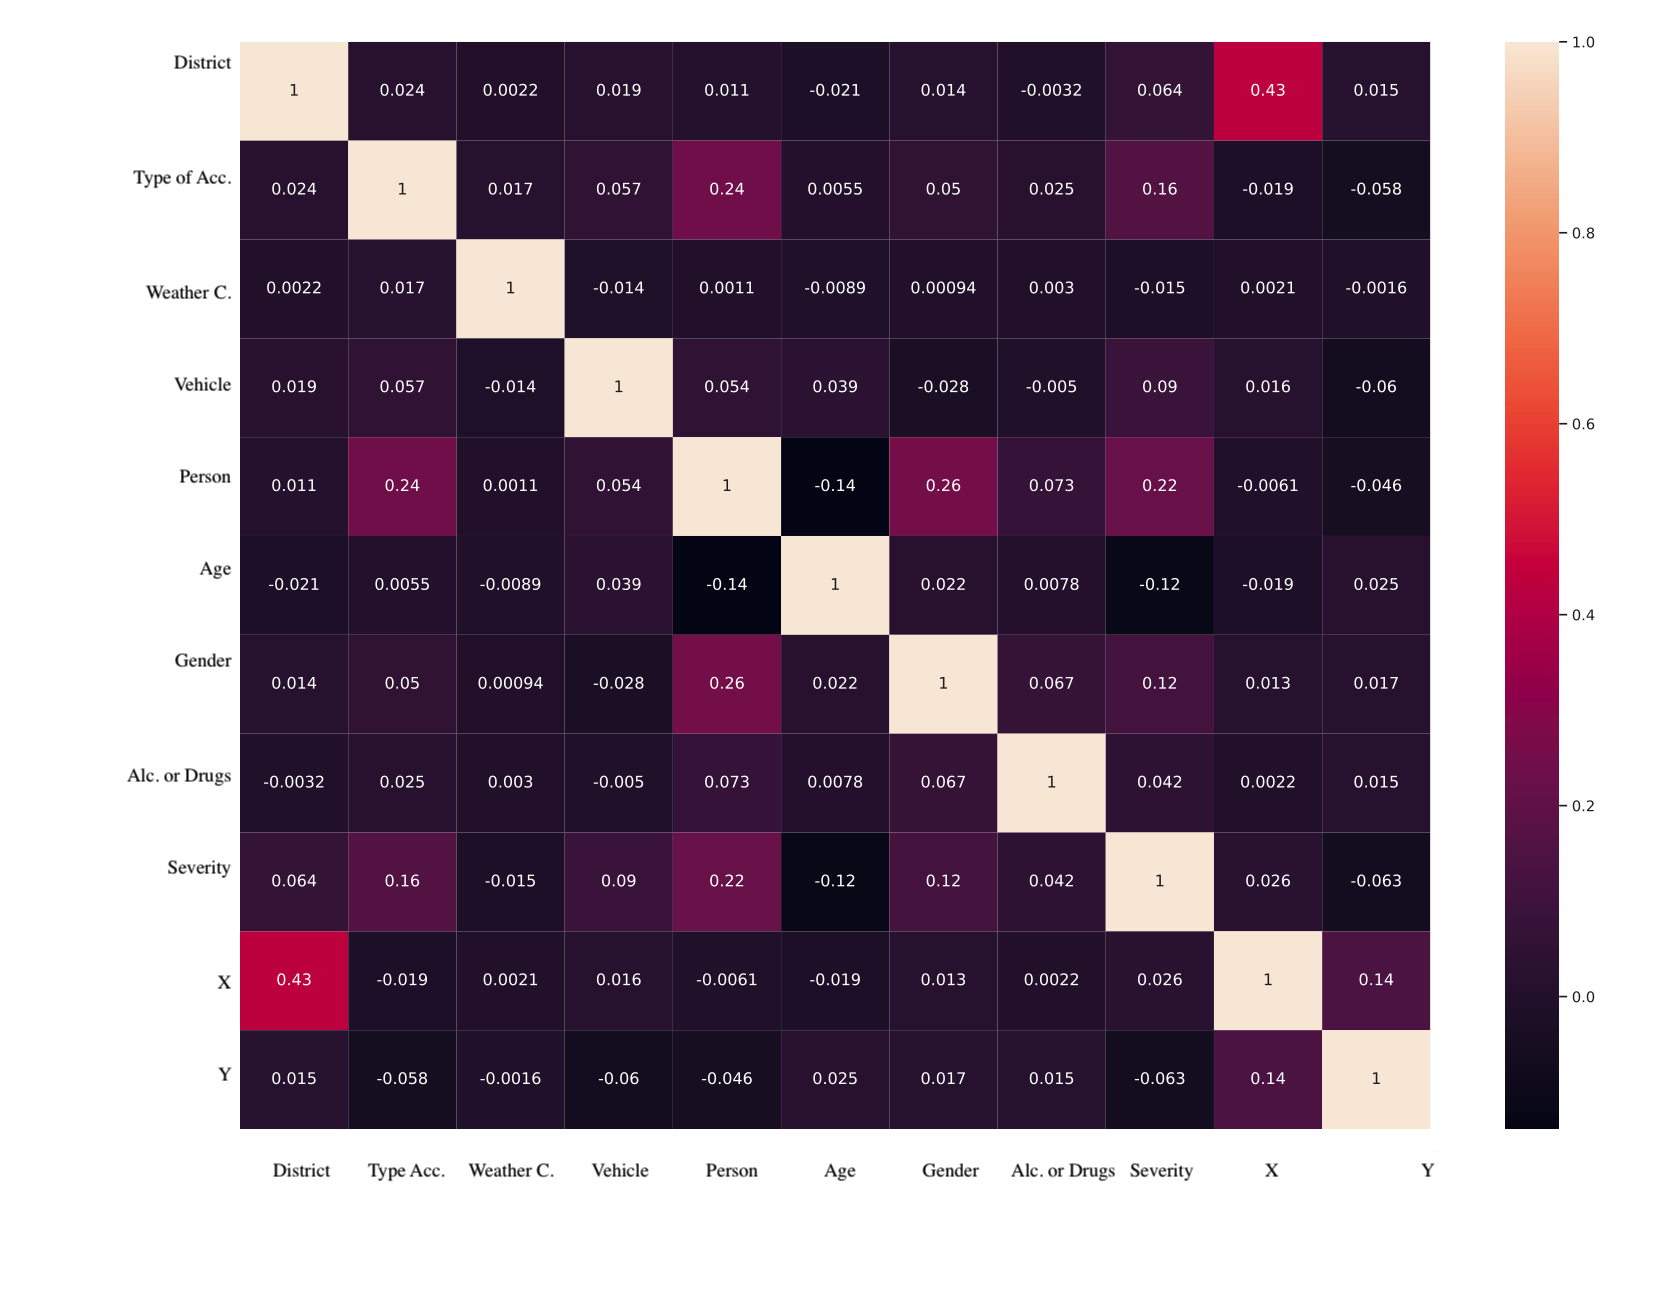
\includegraphics[width=12cm]{Figures/1stPaper/CorrelationMatrix.png}
	\caption{Matriz de correlación entre las variables del conjunto de datos de Madrid}
	\label{CorrelationMatrix}
\end{figure}


\subsection*{Discretización}

Una vez se disponían de los datos refinados y las características adecuadas seleccionadas, era necesario transformar los valores para hacerlos interpretables por los modelos. Este proceso se hizo mediante la asignación de valores numéricos a cada una de las variables cualitativas del dataset en función de la fuerza que representaban los valores de cada característica. Por otra parte, las variables originales \textit{Positivo en Drogas} y \textit{Positivo en Alcohol} se unieron en una nueva característica \textit{Alcohol o Drogas}, con el objetivo de recoger esta información en un único campo y no descartar registros que presentaban valores nulos en ambas columnas. En la Tabla \ref{TransformacionDatosTabla} se muestra la discretización realizada para cada una de las variables.

\textcolor{purple}{Si pones dos columnas en vez de cuatro quedará mejor}
%%%%%%%%%%%%%%%%%%%%%%%%%%%%%%%%%%%%%%%%%%%%%%%%%%%%%%%%%%%%%%%%%%%%%%%%%%%%%%%%%

\begin{table}[H]
	\centering
	\renewcommand{\arraystretch}{1.2}
	\small
	
	\begin{tabular}{|c|l|c|l|}\hline
		\textbf{Característica} & \textbf{Tipificación} & \textbf{Característica} & \textbf{Tipificación} \\ \hline
		\multirow{3}{*}{\textbf{Gravedad}} & 0: Leve (\textit{1, 2, 5, 6, 7}) & \multirow{2}{*}{Tiempo} & 1: Noche (\textit{6 PM - 6 AM}) \\
		& 1: Grave (\textit{3}) & & 2: Día (\textit{6 AM - 6 PM}) \\ \cline{3-4}
		& 2: Fatal (\textit{4}) & Distrito & En base al orden de aparición \\ \hline
		\multirow{1}{*}{X} & Posición Coordenada UTM X & \multirow{12}{*}{Tipo de Accidente} & 1: Colisión frontal \\ \cline{1-2}
		\multirow{1}{*}{Y} & Posición Coordenada UTM Y & & 2: Colisión trasera \\ \cline{1-2}
		\multirow{9}{*}{Tipo de Carretera} & 1: Estacionamiento & & 3: Choque lateral \\
		& 2: Aeropuerto & & 4: Colisión contra obstáculo fijo \\
		& 3: Parque & & 5: Choque en cadena \\
		& 4: Túnel & & 6: Atropello a peatón \\
		& 5: Zona industrial & & 7: Colisión frontal \\
		& 6: Pista & & 8: Otro \\
		& 7: Rotonda & & 9: Salida de la carretera \\
		& 8: Glorieta & & 10: Vuelco de vehículo \\
		& 9: Puerta & & 11: Atropello a animal \\
		& 10: Puente & & 12: Caída \\ \hline
		\multirow{7}{*}{Condiciones Meteorológicas} & 1: Soleado & \multirow{1}{*}{Vehículo} & En base al orden de aparición \\ \cline{3-4}
		& 2: Nublado & \multirow{3}{*}{Persona} & 1: Conductor \\
		& 3: Lluvia ligera & & 2: Pasajero \\
		& 4: Lluvia intensa & & 3: Peatón \\ \cline{3-4}
		& 5: Granizo & \multirow{5}{*}{Edad} & 1: Menos de 18 años \\
		& 6: Nevando & & 2: De 18 a 25 años \\
		& 7: Desconocido & & 3: De 25 a 65 años \\ \cline{1-2}
		\multirow{3}{*}{Género} & 1: Masculino & & 4: Más de 65 años \\
		& 2: Femenino & & 5: Desconocida \\ \cline{3-4}
		& 3: Desconocido & \multirow{1}{*}{Alcohol o Drogas} & 1: Sí / 2: No\\ \hline
	\end{tabular}
	
	\caption{Asignación numérica de las variables del conjunto de datos}
	\label{TransformacionDatosTabla}
\end{table}

%%%%%%%%%%%%%%%%%%%%%%%%%%%%%%%%%%%%%%%%%%%%%%%%%%%%%%%%%%%%%%%%%%%%%%%%%%%%%%%%%

\subsection*{División de datos}


Como es habitual en el diseño de los modelos predictivos, es común dividir los datos en subconjuntos para el aprendizaje de los modelos y su evaluación real sobre registros que nunca ha visto. Del total de muestras resultantes del proceso de filtrado ($65\,158$) se asignan el 80\% de ellas para el conjunto de entrenamiento ($54\,211$), resultando en $53\,213$ accidentes leves, $984$ graves y $50$ fatales. El $20\%$ de los datos restantes se asignaron al conjunto validación o test ($10\,911$), concretamente $10\,640$ accidentes leves, $256$ graves y $15$ fatales.

\subsection*{Normalización}

% \textcolor{red}{\textbf{Luis: Inquietud} Si pongo un ejemplo de normalización random en eta sección, qué pondríamos en resultados GTAAF en esta fase para no repetirnos? Veo lagunas}

% \textcolor{orange}{\textbf{Luis: Propuesta} Lo mencionamos en el resampling como una última frase y listo?}
% \textcolor{purple}{Pon un ejemplo random aquí y en GTAAF se comenta que la normalización es idéntica. Además, deberías poner el rango de normalización}

Una vez aplicado el proceso de limpieza de datos y elección de características del dataset, se aplica la normalización en base a la técnica \textit{Z-Score}, que transformará los datos a una distribución normal con media 0 y desviación 1 de cada valor. Este proceso se aplica para cada una de las muestras de tal forma que la dimensión de los datos quede bajo la misma magnitud, para poder ser  interpretarse eficientemente por los modelos. Una vez se dispone de todos los datos normalizados, pueden ser utilizados para el entrenamiento de cualquier modelo predictivo.


\subsection*{Resampling}


En el punto en el que se disponían de los datos normalizados e interpretables por los modelos, se analizó la distribución final de los datos de entrenamiento en base a la clase a predecir, la gravedad del accidente. Atendiendo a los registros resultantes (Leve, Grave y Fatal), se pudo observar que el conjunto de datos estaba claramente desbalanceado. Se disponían de $53\,213$ accidentes leves, $984$ graves y $50$ fatales. Esto, como se ha comentado en la sección \ref{SOAT_RESAMPLING}, se convierte en un problema para los modelos de clasificación, ya que en estos casos tienden a predecir las nuevas muestras como aquellas que pertenecen a la clase mayoritaria. Para paliar este problema se aplicó la técnica de remuestreo \textit{Borderline SMOTE-II}, con el objetivo de generar más muestras de accidentes pertenecientes a clases minoritarias (Grave y Fatal) hasta llegar a la mayoritaria (Leves), evitando que el modelo se sobreajuste. Una vez aplicado el algoritmo, se disponen de $53\,213$ muestras de la clase leve, $53\,213$ de la clase grave y $53\,213$ de la clase fatal, haciendo un total de $159\,639$ registros en el nuevo conjunto de datos de entrenamiento balanceado.



\subsection*{Categorización}

Como se ha comentado en secciones anteriores, las redes neuronales convolucionales aprenden patrones utilizando matrices como datos de entrada. Así pues, como se disponen de datos tabulares, se hace necesario transformarlos en matrices.

Uno de los requisitos de esta transformación era asignar cada característica a una categoría del dataset. Sobre este conjunto de datos de Madrid, las variables eran asignadas a $5$ categorías en base a la información de la que se disponía: (1) Características del accidente, (2) Condiciones de la carretera, (3) Condiciones meteorológicas, (4) Características del vehículo y (5) Características del conductor. En la Tabla \ref{JC} se observa la categorización de cada característica en función de la información que describen.

% \textcolor{red}{\textbf{Luis: Comentario} Exponer la categorización no me termina de cuadrar aquí, principalmente porque en el siguiente (GTAAF) esto se pone en la descripción de los datos. A lo mejor no está mal dejarlo como está... Porque así el lector le daría más importancia a la categorización en el modelo GTAAF, porque aparece lo primero. No sé, también es verdad que si lo dejamos así queda un poco caótico a la hora de comparar la metodología preliminar y la GTAAF. Siento el rollo, hay alguna opinión? :-(}

% \textcolor{purple}{Lo dejamos así y cuando se explique GTAAF hay que decir que esta categorización es fundamental para generalizar el modelo por eso se explica en la descripciónd e los datos.}


% \textcolor{red}{\textbf{Luis: CUIDADO} En el paper 1 en esta tabla se pone severidad dentro de accidente... y no es el único sitio. Es posible solicitar correcciones del otro paper?}
% \textcolor{green}{MANU: se que se puede de alguna forma, pero nunca lo he hecho...}

\begin{table}[H]
	\centering
	
	\begin{tabular}{ |c|c| }
		\hline
		\textbf{Categoría} & \textbf{Característica} \\
		\hline
		\hline
		\multirow{5}{*}{Accidente} & X \\
		& Y \\
		& Hora \\
		& Tipo de accidente \\
		& Vehículos implicados \\
		\hline
		\hline
		\multirow{2}{*}{Carretera} & Tipo de carretera \\
		& Distrito \\
		\hline
		\hline
		Clima & Condiciones climáticas \\
		\hline
		\hline
		Vehículo & Tipo de Vehículo \\
		\hline
		\hline
		\multirow{4}{*}{Conductor}  & Tipo de Persona \\
		& Género \\
		& Edad \\
		& Alcohol o Drogas \\
		\hline
		\hline
	\end{tabular}
	
	\caption{Clasificación de características (variables del conjunto de datos) en categorías. Modelo Preeliminar}
	\label{JC}
\end{table}



\subsection*{Algoritmo Genético}

% \textcolor{red}{\textbf{Luis: CUIDADO} En el paper 1 dijimos que se optimizaron cinco hiperparámetros del XGBoost cuando esto es falso. Aquí he puesto la realidad. Qué hacemos?}

% \textcolor{purple}{Déjalo como está, no creo que nadie se mire el paper 1 para comparar. Si te preguntan en el tribunal, puedes decir que al principio se optimizaron 5 pero que el resultado de 2 de ellos siempre era el mismo, con lo que se decidió optimizar solo 3}

En este punto, se analiza la optimización de los hiperparámetros del algoritmo \textit{XGBoost} a través del algoritmo genético mediante la maximización de la métrica \textit{F1-Score} de los datos de entrenamiento. Los hiperparámetros del algoritmo \textit{XGBoost} a optimizar fueron: profundidad máxima del árbol, peso mínimo de los hijos y el ratio de aprendizaje. El algoritmo genético se configuró para optimizar esta función durante $80$ generaciones, con un máximo de $40$ individuos en la población y los $10$ mejores en cada iteración eran seleccionados para reproducirse mediante una estrategia de cruce aleatorio.

La figura \ref{EvolucionHiperparametrosImage} muestra la evolución de  los tres hiperparámetros del \textit{XGBoost} a lo largo de las generaciones. Como se puede observar, los hiperparámetros toman distintos valores en función del mejor individuo evaluado en la población en cada etapa, estos hiperparámetros convergían aproximadamente en la iteración $42$, donde no se observaron incrementos en este métrica a partir de esta generación.

\begin{figure}[H]
	\centering
	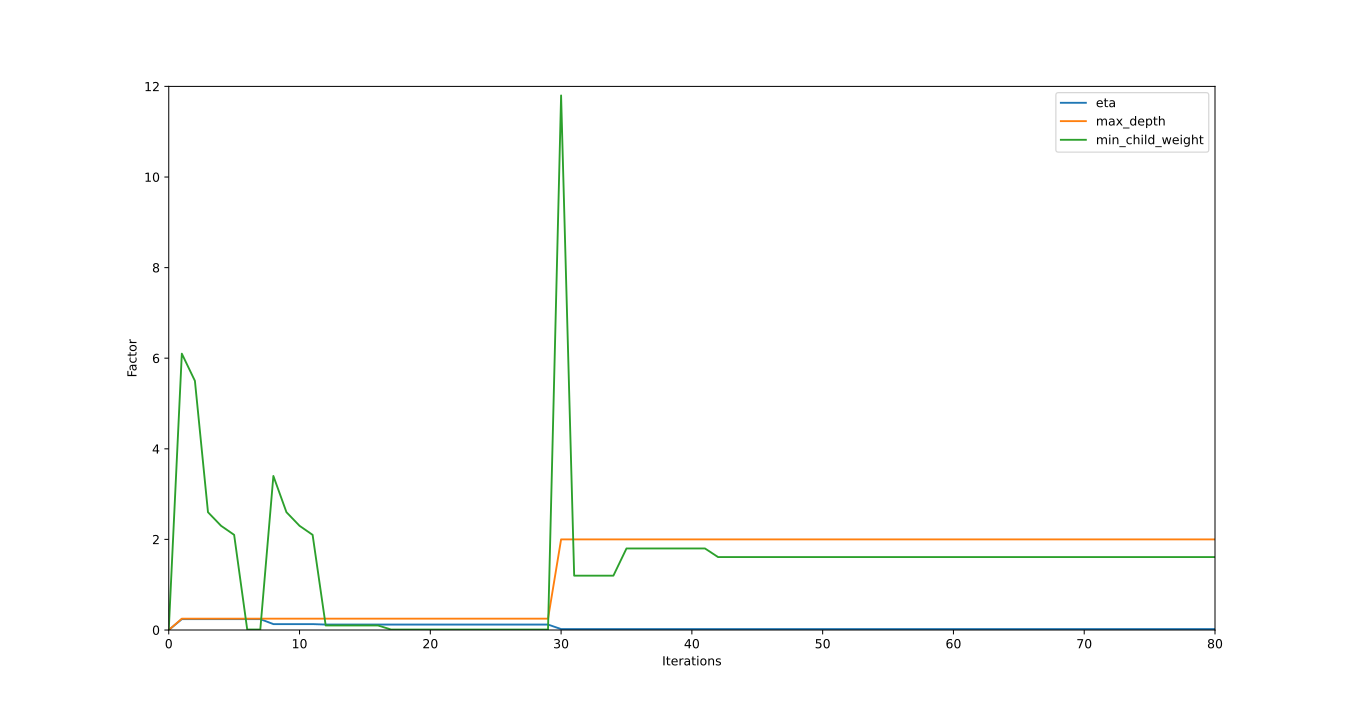
\includegraphics[width=14cm]{Figures/1stPaper/EvolutionH.png}
	\caption{Evolución de los hiperparámetros del \textit{XGBoost} a lo largo de las generaciones}
	\label{EvolucionHiperparametrosImage}
\end{figure}

En la tabla \ref{BestGASolutionTable} se observa el valor tomado por el mejor individuo resultante de la ejecución de las distintas generaciones para cada uno de los hiperparámetros del \textit{XGBoost}. 

%%%%%%%%%%%%%%%%%%%%%%%%%%%%%%%%%%%%%%%%%%%%%%%%%%%%%%%%%%%%%%%%%%%%%%%%%%%%%%%%%
\begin{table}[h]
	\caption{Valores optimizados de los parámetros del \textit{XGBoost} después de aplicar el algoritmo genético del modelo preliminar}
	\centering
	\begin{tabular}{ |c|c| } 
		\hline
		\textbf{Hiperparámetro} & \textbf{Valor}\\
		\hline
		Profundidad Máxima & 2 \\
		Peso Mínimo de Hijos & 1.6 \\ 
		ETA & 0.007 \\
		\hline
	\end{tabular}

	\label{BestGASolutionTable}
\end{table}
%%%%%%%%%%%%%%%%%%%%%%%%%%%%%%%%%%%%%%%%%%%%%%%%%%%%%%%%%%%%%%%%%%%%%%%%%%%%%%%%%

%\underline{Pesos de categorías}

Con la configuración de hiperparámetros mostrada en la Tabla \ref{BestGASolutionTable} se entrena el algoritmo \textit{XGBoost} para obtener el peso de todas las  características del conjunto de datos. Así, en la Tabla \ref{1stPaperWeightsFinalCharacteristics} se muestra el peso asignado a cada una de las características individuales, donde la columna peso de la Categoría muestra el peso de cada categoría como suma de los peso de cada una de las características individuales que la componen.

% \textcolor{red}{\textbf{Luis: CUIDADO} En el paper 1 en esta tabla se pone severidad dentro de accidente... y no es el único sitio. Es posible solicitar correcciones del otro paper?}

%%%%%%%%%%%%%%%%%%%%%%%%%%%%%%%%%%%%%%%%%%%%%%%%%%%%%%%%%%%%%%%%%%%%%%%%%%%%%%%%%
\begin{table}[ht]
	\caption{Ejemplo con los pesos de todas las características estudiadas, así como los pesos de las cinco categorías}
	\centering
	\begin{tabular}{ |c|c||c|c| }
		\hline
		\textbf{Categoría} & \textbf{Peso} & \textbf{Característica} & \textbf{Peso}\\
		\hline
		\hline
		\multirow{5}{*}{Accidente}   & \multirow{5}{*}{0.299} & Coordenada X & 0.071\\
		&  & Coordenada Y  & 0.066\\
		&  & Hora & 0.055\\
		&  & Tipo de accidente  & 0.051\\
		&  & Vehículos implicados & 0.057\\
		\hline
		
		\multirow{2}{*}{Carretera} & \multirow{2}{*}{0.187} & Distrito  & 0.059\\      
		&  & Tipo de Carretera & 0.127\\
		\hline
		
		\multirow{1}{*}{Clima}  & \multirow{1}{*}{0.050}  & Condiciones Climáticas  & 0.050\\
		\hline
		
		\multirow{1}{*}{Vehículo}  & \multirow{1}{*}{0.070} & Tipo de Vehículo  & 0.070\\
		\hline
		
		\multirow{4}{*}{Conductor}   & \multirow{4}{*}{0.394} & Tipo de Persona & 0.177\\
		&      & Género      & 0.111\\
		&      & Edad      & 0.050\\
		&      & Alcohol o Drogas  & 0.056\\
		\hline
		
	\end{tabular}

	\label{1stPaperWeightsFinalCharacteristics}
\end{table}

\subsection*{Construcción de matrices}


Una vez se disponían de las características y categorías evaluadas, se aplicaba el proceso de asignación de posiciones de cada característica a las respectivas coordenadas dentro de la matriz, aplicando el algoritmo de construcción de matrices.

En la Tabla \ref{ProcesoMatriz:Array} se observa un ejemplo de un registro transformado a formato matricial una vez se ha aplicado el algoritmo de construcción haciendo uso de la importancia de las características de la tabla \ref{1stPaperWeightsFinalCharacteristics}. Igualmente, en la figura \ref{ProcesoMatriz:VisualizacionDeMatriz}, se observa la representación en imagen de escala de grises de dicha matriz.


\begin{table}[H]
	\caption{Matriz resultante tras la transformación de un registro a formato matricial. Las filas representan las categorías y las columnas las características que la componen, ordenadas en función de los pesos mediante el criterio presentado en la sección \ref{METODOLOGIA_MODELO_PRELIMINAR}}
	\begin{center}
		\begin{tabular}{|c|c|c|c|c|}
			\hline
			$0.0$ & $0.0$ &  $-0.1621$  & $0.0$ & $0.0$\\
			$1.2548$ & $0.0081$ &  $-0.0524$  & $-1.4528$ & $-1.4591$\\
			$0.2129$ & $-0.7004$ &  $-0.5316$  & $0.1488$ & $0.0$\\
			$0.0$ & $-0.0297$ &  $0.4597$  & $0.0$ & $0.0$\\
			$0.0$ & $0.0$ &  $-0.2508$  & $0.0$ & $0.0$\\
			\hline
		\end{tabular}
	\end{center}

	\label{ProcesoMatriz:Array}
\end{table}

\begin{figure}[H]
	\centering
	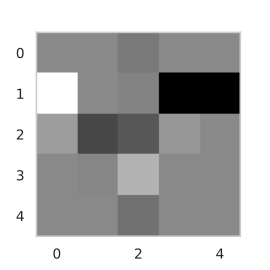
\includegraphics[width=6cm]{Figures/TFM/accidente_fatal.png}
	\caption{Imagen de la matriz en escala de grises.}
	\label{ProcesoMatriz:VisualizacionDeMatriz}
\end{figure}


%\begin{figure}[H]
%   \centering
%   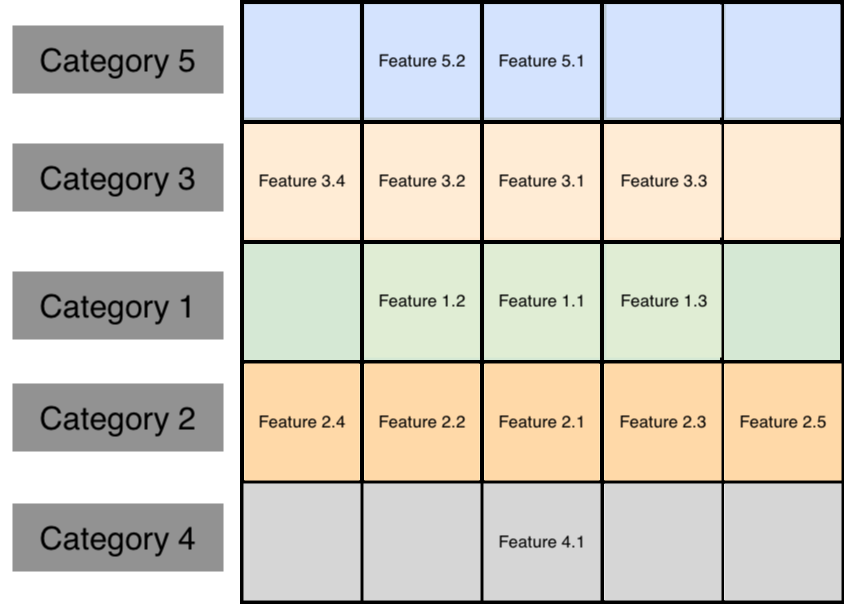
\includegraphics[width=10cm]{Figures/1stPaper/FV2I.png}
%   \caption{Example of positioning the elements in a matrix. Categories are assigned in rows based on their weight, and Features are assigned in the columns of the corresponding category based on their weight.}
%   \label{FV2IExample}
%\end{figure}

\subsection*{Entrenamientos}

Una vez que las matrices han sido construidas, se describe la red convolucional utilizada en el modelo propuesto. En esta sección se presenta la información resultante de los entrenamientos realizados para los dos modelos convolucionales, de una y dos dimensiones, sobre los que trabaja el modelo preliminar. De esta forma se analizará la evolución de la función de pérdida en cada uno de estos modelos. Ambos fueron entrenados con $100$ épocas, al analizar la evolución del entrenamiento de la red convolucional unidimensional (CNN-1D), se puedo verificar que la puntuación \textit{F1-Score} de entrenamiento incrementaba ínfimamente a lo largo de las épocas, sufriendo además altibajos sobre el conjunto de validación a medida que el modelo se entrenaba, comenzando inicialmente con un valor de entrenamiento inferior a $0.58$ y llegando hasta $0.68$, mostrando poca capacidad de aprendizaje y generalización ante nuevas muestras.

Por otro lado, sobre el modelo convolucional bidimensional (CNN-2D) observó que la tendencia de la función de pérdida en el conjunto de datos de entrenamiento era más estable. Se pudo comprobar cómo la red, en la primera ejecución, comenzaba con una puntuación \textit{F1-Score} de $0.62$ hasta alcanzar $0.78$ en la iteración $100$, por lo que se puedo deducir que esta red lograba un mejor rendimiento en el conjunto de entrenamiento en comparación con la red convolucional unidimensional, sufriendo menos altibajos en el conjunto de validación.


\subsection*{Evaluación}

% \textcolor{red}{\textbf{Luis: quitaría incluso el análisis de los datos de entrenamiento}}

Para evaluar el rendimiento del modelo preeliminar, se realizó una comparación con tres modelos del estado del arte, \textit{Gaussian Naive Bayes (GNB), Support Vector Classifier (SVC)} y \textit{K-Nearest Neighbor (KNN)}. En esta sección se utilizarán las métricas obtenidas tras la ejecución de los cinco modelos sobre el conjunto de datos de test (\textit{CNN-1D, CNN-2D, GNB, SVC} y \textit{KNN}).

Las Tablas \ref{ClassificationReportCNN:TrainCNN} y \ref{ClassificationReportCNN:TestCNN} detallan las métricas resultantes de la clasificación de las redes para los conjuntos de entrenamiento y test respectivamente. Se observó que, para el conjunto de entrenamiento, el modelo CNN-1D obtenía un mejor \textit{F1-Score} en la clasificación de todas las clases de accidentes en comparación con la red CNN-2D. Sin embargo, al analizar las métricas de los datos de test, el modelo que presentaba mejor \textit{F1-Score} para accidentes leves y graves era el CNN-2D, con $0.950$ y $0.148$ respectivamente, mientras que en accidentes fatales ambas redes ofrecían el mismo rendimiento con un $0.004$ de \textit{F1-Score}.

\begin{table}[H]
	\caption{Métricas sobre el conjunto de entrenamiento para los modelos CNN-1D y CNN-2D}
	\begin{center}
		\begin{tabular}{|c||c|c|c||c|c|c|}
			\hline
			\multicolumn{1}{ |c|| }{} & \multicolumn{3}{ |c|| }{\textbf{CNN-1D}} & \multicolumn{3}{ |c| }{\textbf{CNN-2D}} \\ \hline
			\textbf{Métrica/Gravedad} & Leve & Grave & Fatal & Leve & Grave & Fatal
			\\ \hline \hline 
			Precision & 0.701 & 0.696 & 0.754 & 0.488 & 0.646 & 0.966 \\ \hline 
			Recall & 0.724 & 0.523 & 0.917 & 0.974 & 0.299 & 0.524\\ \hline 
			F1-score & 0.712 & 0.597 & 0.828 & 0.650 & 0.409 & 0.679\\ \hline 
		\end{tabular}
	\end{center}

	\label{ClassificationReportCNN:TrainCNN}
\end{table}

\begin{table}[H]
	\caption{Métricas sobre el conjunto de test para los modelos CNN-1D y CNN-2D}
	\begin{center}
		\begin{tabular}{|c||c|c|c||c|c|c|}
			\hline
			\multicolumn{1}{ |c|| }{} & \multicolumn{3}{ |c|| }{\textbf{CNN-1D}} & \multicolumn{3}{ |c| }{\textbf{CNN-2D}} \\ \hline
			\textbf{Métrica/Gravedad} & Leve & Grave & Fatal & Leve & Grave & Fatal
			\\ \hline \hline 
			Precision & 0.984 & 0.031 & 0.002 & 0.982 & 0.097 & 0.002\\ \hline 
			Recall & 0.429 & 0.394 & 0.333 & 0.919 & 0.313 & 0.1\\ \hline 
			F1-score & 0.596 & 0.058 & 0.004 & 0.950 & 0.148 & 0.004\\ \hline 
		\end{tabular}
	\end{center}

	\label{ClassificationReportCNN:TestCNN}
\end{table}

% \textcolor{red}{\textbf{Luis: Percepción} me da la sensación de que hay mucho contenido aquí. La forma de exponer los resultados (primero los de las CNNs y luego los modelos del estado del arte) provoca que esto sea muy largo cuando en mi opinión, estos resultados no tienen mucha importancia. Lo reestructuramos o qué pensais?}

% \textcolor{purple}{Jose: Tienes razón, se me está haciendo un poco pesado de leer, lo que significa que deberíamos reducirlo. ¿Quitamos lo referente a las matrices de confusión y lo centramos en los resultados del F1-score?}

% \textcolor{orange}{Luis: Me parece buena idea, he quitado lo relativo a las matrices. Además creo que deberíamos reducir todo lo referente a los resultados preliminares..}

% La Figura \ref{ConfusionMatricesImages} muestra las matrices de confusión para los conjuntos de entrenamiento y test de ambos modelos, donde se pueden analizar las tendencias predictivas. Para los datos de entrenamiento de CNN-2D, tendía a una mayor propensión de predecir observaciones como accidentes leves en comparación con la red CNN-1D. Esto provocaba que la CNN-1D clasificase correctamente más accidentes graves y fatales. Para el conjunto de datos de test, la red CNN-2D clasificaba más observaciones como accidentes leves que el modelo CNN-1D, prediciendo menos accidentes graves pero con mayor confianza.

% %%%%%%%%%%%%%%%%%%%%%%%%%%%%%%%%%%%%%%%%%%%%%%%%
% \begin{figure}[H]
	%     \centering
	%     \subfigure[Training CNN-1D]{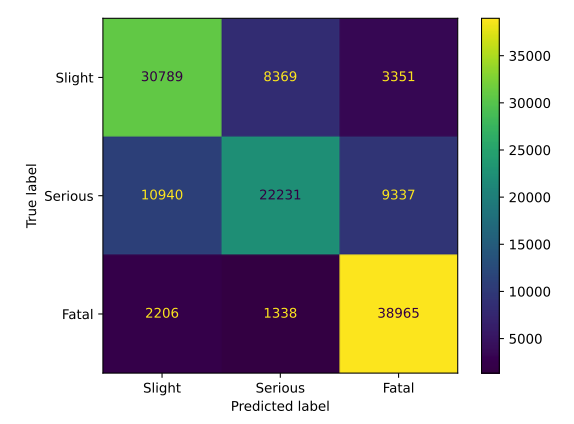
\includegraphics[width=60mm]{Figures/1stPaper/1DConfusionMatrixTrain}}
	%     \subfigure[Training CNN-2D]{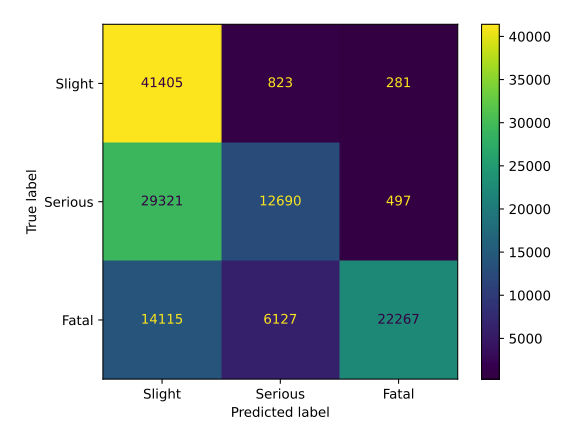
\includegraphics[width=60mm]{Figures/1stPaper/2DConfusionMatrixTrain}}
	%     \subfigure[Test CNN-1D]{\includegraphics[width=60mm]{Figures/1stPaper/1DConfusionMatrixTest}}
	%     \subfigure[Test  CNN-2D]{\includegraphics[width=60mm]{Figures/1stPaper/Diagrama sin título.drawio}}
	%     \caption{Matrices de confusión de entrenamiento y test para las redes neuronales convolucionales.}
	%     \label{ConfusionMatricesImages}
	% \end{figure}
% %%%%%%%%%%%%%%%%%%%%%%%%%%%%%%%%%%%%%%%%%%%%%%%%


La información con la que se evalúan los modelos, es decir, las métricas de clasificación resultantes para el conjunto de test se muestran en la Tabla \ref{ClassificationReportCNN:Test} para cada una de las clases predichas. Como se puede ver en esta tabla, el modelo \textit{KNN} obtiene mejores resultados en todas las medidas de todas las clases, excepto en \textit{Recall} en accidentes graves, donde el \textit{GNB} es un ligeramente mejor.

Si analizamos la métrica de \textit{Precision} en los cinco modelos comparados, se puede observar que el modelo que presenta el mejor promedio para las clases de accidentes leves es la Red Neuronal Convolucional 1D (CNN-1D) con $0.984$, seguida por la Red Neuronal Convolucional 2D (CNN-2D) y el modelo \textit{KNN} con $0.982$. Además, la CNN-2D también ofrece la mejor métrica para accidentes graves, $0.097$, con una gran diferencia respecto al modelo que le sigue, \textit{KNN} con $0.042$. En cuanto a los accidentes fatales, ambos modelos CNN-1D y CNN-2D tienen un valor similar, obteniendo $0.002$.

Con respecto a la métrica de \textit{Recall}, el mejor promedio para las clases de accidentes leves es la Red Neuronal Convolucional 2D (CNN-2D) con $0.919$, seguida por el modelo \textit{KNN} con $0.689$. Además, el modelo \textit{GNB} ofrece la mejor métrica para accidentes graves, $0.699$. En accidentes fatales, CNN-2D presenta el mejor valor con $0.1$.

Es necesario señalar que el \textit{F1-score} es una forma de combinar las métricas de \textit{Precision} y \textit{Recall}, y se define como la media armónica de ambas. Teniendo esto en cuenta, analizando el \textit{F1-Score} de los reportes, el modelo que presenta el mejor promedio para las clases de accidentes leves es la red CNN-2D, alcanzando $0.950$, muy por encima del siguiente modelo \textit{KNN}, que ofrece un valor de $0.810$. Además, la CNN-2D también ofrece la mejor métrica para accidentes graves, $0.148$, alcanzando el doble de rendimiento en comparación con el modelo que le sigue, \textit{KNN} con $0.076$. En cuanto a los accidentes fatales, los modelos con mejor clasificación son tanto la CNN-1D como la CNN-2D, obteniendo $0.004$, el doble que \textit{KNN}, que son los siguientes mejores modelos en esta clase con $0.002$.

Podemos concluir que el modelo preliminar propuesto, basado en redes neuronales convolucionales (CNN-1D y CNN-2D), presentaba mejores predicciones con respecto a la métrica \textit{F1-score}, aunque con gran potencial de mejora.

\begin{table}[H]
	\caption{Métricas de clasificación sobre el conjunto de test de los modelos \textit{GNB}, \textit{SVC} y \textit{KNN} en comparación con el modelo preliminar.}
	\begin{center}
		\begin{tabular}{|c||c|c|c|}
			\hline
			 \multicolumn{4}{ |c| }{\textbf{GNB}} \\
			  \hline \hline
			\textbf{Métrica/Gravedad} & Leve & Grave & Fatal \\  \hline 
			Precision & 0.980 & 0.025 & 0  \\ \hline 
			Recall & 0.369 & 0.699 & 0  \\ \hline 
			F1-score & 0.536 & 0.048 & 0 \\ \hline
			 \multicolumn{4}{ c }{} \\ 
			 
			 \hline
			 \multicolumn{4}{ |c| }{\textbf{SVC}} \\ 
			 \hline \hline
			\textbf{Métrica/Gravedad} & Leve & Grave & Fatal \\  \hline 
			Precision  & 0.979 & 0.029 & 0  \\ \hline 
			Recall  & 0.644 & 0.411 & 0  \\ \hline 
			F1-score & 0.777 & 0.054 & 0 \\ \hline
			\multicolumn{4}{ c }{} \\ 
			
			\hline
			\multicolumn{4}{ |c| }{\textbf{KNN}} \\ 
			\hline \hline
			\textbf{Métrica/Gravedad} & Leve & Grave & Fatal \\  \hline 
			Precision & 0.982 & 0.042 & 0.001 \\ \hline 
			Recall & 0.689 & 0.382 & 0.067 \\ \hline 
			F1-score  & 0.810 & 0.076 & 0.002\\ \hline 
		\end{tabular}
	\end{center}
	\label{ClassificationReportCNN:Test}
\end{table}


% \textcolor{purple}{Jose: ¿Quitamos lo de las matrices de confusión en este apartado?}

% \textcolor{orange}{Luis: Quitado}

% La Figura \ref{ClassificationReportCNN:Test} muestra las matrices de confusión aplicadas al conjunto de prueba, presentando una representación visual de las métricas de clasificación. Esto permite abordar el hecho de que los modelos GNB y SVC no clasifican correctamente ninguna de las observaciones de accidentes fatales, mientras que KNN clasifica una. En cuanto a los accidentes leves, el modelo CNN-2D es el que clasifica correctamente el mayor número, al igual que en los accidentes graves. Esto se debe a la naturaleza de las redes aplicadas a la complejidad del problema, cada una de ellas encuentra patrones diferentes según los mapas característicos resultantes de las convoluciones de cada red.


% % \textcolor{red}{\textbf{Luis: CUIDADO} Cuidado con el CNN-2D test, el nº de muestras de accidentes fatales no concuerda con el resto. Sigo sin saber cómo nos aprobaron ese paper.}

% %%%%%%%%%%%%%%%%%%%%%%%%%%%%%%%%%%%%%%%%%%%%%%%%
% \begin{figure}[H]
	% \centering
	% %\subfigure[Training CNN-1D]{\includegraphics[width=70mm]{Figures/1DConfusionMatrixTest}}
	% %\subfigure[Training CNN-2D]{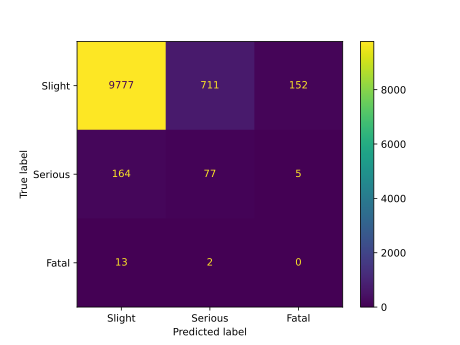
\includegraphics[width=70mm]{Figures/2DConfusionMatrixTest}}
	% \subfigure[Test GNB]{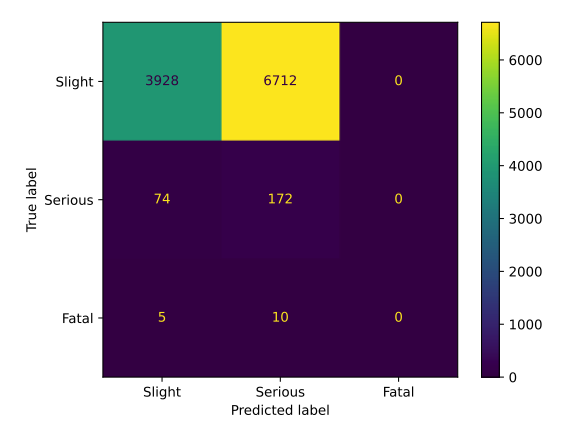
\includegraphics[width=60mm]{Figures/1stPaper/NBConfusionMatrixTest.png}}
	% \subfigure[Test KNN]{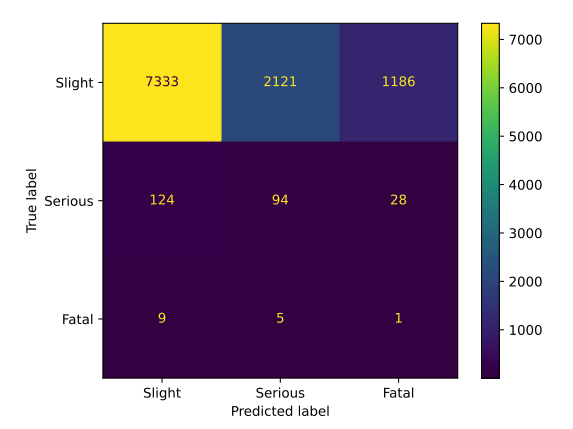
\includegraphics[width=60mm]{Figures/1stPaper/KNNConfusionMatrixTest.png}}
	% \subfigure[Test SVC]{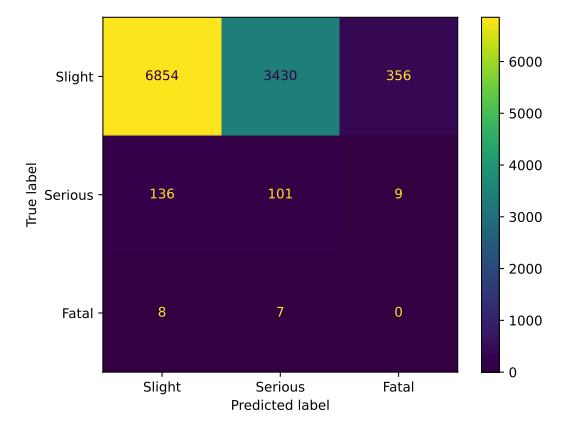
\includegraphics[width=60mm]{Figures/1stPaper/SVCConfusionMatrixTest.png}}
	% \caption{Matrices de confusión aplicadas para el conjunto de test de los modelos GNB, SVC y KNN.}
	% \label{ConfusionMatrixCNNImages}
	% \end{figure}
% %%%%%%%%%%%%%%%%%%%%%%%%%%%%%%%%%%%%%%%%%%%%%%%%

% Como se puede observar en los resultados de los experimentos, las dos arquitecturas convolucionales propuestas superan al resto de los modelos de referencia para cada una de las clases de accidentes (Leves, Graves y Fatales). La ventaja de contar con estas dos nuevas arquitecturas es que cada una de ellas funciona mejor según el tipo de clase que se va a predecir. Esto permite el diseño de un sistema en el cual las dos redes entrenadas se utilicen para combinar sus resultados, de manera que la red CNN-1D se usaría para predecir accidentes leves y fatales, mientras que la red CNN-2D clasificaría accidentes graves.

\subsection*{Discusión de resultados del modelo preliminar}

% \textcolor{red}{\textbf{Luis: } esto es realmente lo mismo que la introducción al modelo GTAAF pero más justificado en base al análisis de resultados, no sé si estaría bien repetirse.}

% \textcolor{purple}{\textbf{Jose: Aquí pondría esto}}

Analizando los resultados finales de este modelo preliminar se propusieron una serie de mejoras a desarrollar para crear un modelo general en la gravedad de los accidentes de tráfico, aportando así un posible valor a las administraciones públicas para asignar recursos médicos en los accidentes de tráfico. En primer lugar, se detectó que la decisión de disgregar la clasificación de la gravedad de los accidentes en tres clases provocaba un efecto conflictivo en la clasificación de los modelos debido a que dos de las clases en las que se dividía la gravedad de los accidentes eran minoritarias, lo que penalizaba el aprendizaje del modelo. Por otra lado, al intentar generalizar el modelo, la adaptación del modelo para poder aplicarla en cualquier conjunto de datos era prioritaria. De esta forma, cualquier información que pudiese ser relevante en la predicción de la gravedad de los accidentes, orientado a la falta de disponibilidad de datos en cada región, debería ser añadida. Finalmente se comprobó que había datos ya existentes de los que se podían sacar más características importantes. Por ejemplo, la hora del accidente no estaba representada debido a su naturaleza cíclica. Todos estas debilidades hicieron necesario la implantación de soluciones que aportaran generalidad al modelo definitivo.

% \textcolor{purple}{\textbf{Jose: Los siguientes párrafos los pasaría al modelo definitivo, al principio de la sección siguiente}}


%%%%%%%%%%%%%%%%%%%%%%%%%%%%%%%%%%%%%%%%%%%%%%%%%%%%%%%%%%%%%%%%%%%%%%%%%%%%%%%%%%%%%%%%%%%%%%%%%%%%%%%%%%%%%%%%%%%%%%%%%%%%%%%%%%%%%%%%%%%%%%%%%%%%%%%%%%%%%%%%%%%%%%%%%%%%%%%%%%%%%%%%%%%%%%%%%%%%%%%%%%%%%%%%%%%%%%%%%%%%%%%%%%%%%%%%%%%%%%%%%%%%%%%%%%%%%%%%%%%%%%%%%%%%%%%%%%%%%%%%%%%%%%%%%%%%%%%%%%%%%%%%%%%%%%%%%%%%%%%%%%%%%%%%%%%%%%%%%%%%%%%%%%%%%%%%%%%%%%%%%%%%%%%%%%%%%%%%%%%%%%%%%%%%%%%%%%%%%%%%%%%%%%%%%%%%%%%%%%%%%%%%%%%%%%%%%%%%%%%%%%%%%%%%%%%%%%%%%%%%%%%%%%%%%%%%%%%%%%%%%%%%%%%%%%%%%%%%%%%%%%%%%%%%%%%%%%%%%%%%%%%%%%%%%%%%%%%%%%%%%%%%%%%%%%%%%%%%%%%%%%%%%%%%%%%%%%%%%%%%%%%%%%%%%%%%%%%%%%%%%%%%%%%%%%%%%%%%%%%%%%%%
%%%%%%%%%%%%%%%%%%%%%%%%%%%%%%%%%%%%%%%%%%%%%%%%%%%%%%%%%%%%%%%%%%%%%%%%%%%%%%%%%%%%%%%%%%%%%%%%%%%%%%%%%%%%%%%%%%%%%%%%%%%%%%%%%%%%%%%%%%%%%%%%%%%%%%%%%%%%%%%%%%%%%%%%%%%%%%%%%%%%%%%%%%%%%%%%%%%%%%%%%%%%%%%%%%%%%%%%%%%%%%%%%%%%%%%%%%%%%%%%%%%%%%%%%%%%%%%%%%%%%%%%%%%%%%%%%%%%%%%%%%%%%%%%%%%%%%%%%%%%%%%%%%%%%%%%%%%%%%%%%%%%%%%%%%%%%%%%%%%%%%%%%%%%%%%%%%%%%%%%%%%%%%%%%%%%%%%%%%%%%%%%%%%%%%%%%%%%%%%%%%%%%%%%%%%%%%%%%%%%%%%%%%%%%%%%%%%%%%%%%%%%%%%%%%%%%%%%%%%%%%%%%%%%%%%%%%%%%%%%%%%%%%%%%%%%%%%%%%%%%%%%%%%%%%%%%%%%%%%%%%%%%%%%%%%%%%%%%%%%%%%%%%%%%%%%%%%%%%%%%%%%%%%%%%%%%%%%%%%%%%%%%%%%%%%%%%%%%%%%%%%%%%%%%%%%%%%%%%%%%%%%%%%%%%%%%%%%%%%%%%%%%%%%%%%%%%%%%%%%%%%%%%%%%%%%%%%%%%%%%%%%%%%%%%%%%%%%%%%%%%%%%%%%%%%%%%%%%%%%%%%%%%%%%%%%%%%%%%%%%%%%%%%%%%%%%%%%%%%%%%%%%%%%%%%%%%%%%%M Me he quedado  por aquí %%%%%%%%%%%%%%%%%%%%%%%%%%%%%%%%%%%%%%%%%%%%%%%%%%%%%%%%%%%%%%%%%%%%%%%%%%%%%%%%%%%%%%%%%%%%%%%%%%%%%%%%%%%%%%%%%%%%%%%%%%%%%%%%%%%%%%%%%%%%%%%%%%%%%%%%%%%%%%%%%%%%%%%%%%%%%%%%%%%%%%%%%%%%%%%%%%%%%%%%%%%%%%%%%%%%%%%%%%%%%%%%%%%%%%%%%%%%%%%%%%%%%%%%%%%%%%%%%%%%%%%%%%%%%%%%%%%%%%%%%%%%%%%%%%%%%%%%%%%%%%%%%%%%%%%%%%%%%%%%%%%%%%%%%%%%%%%%%%%%%%%%%%%%%%%%%%%%%%%%%%%%%%%%%%%%%%%%%%%%%%%%%%%%%%%%%%%%%%%%%%%%%%%%%%%%%%%%%%%%%%%%%%%%%%%%%%%%%%%%%%%%%%%%%%%%%%%%%%%%%%%%%%%%%%%%%%%%%%%%%%%%%%%%%%%%%%%%%%%%%%%%%%%%%%%%%%%%%%%%%%%%%%%%%%%%%%%%%%%%%%%%%%%%%%%%%%%%%%%%%%%%%%%%%%%%%%%%%%%%%%%%%%%%%%%%%%%%%%%%%%%%%%%%%%%%%%%%%%%%%%%%%%%%%%%%%%%%%%%%%%%%%%%%%%%%%%%%%%%%%%%%%%%%%%%%%%%%%%%%%%%%%%%%%%%%%%%%%%%%%%%%%%%%%%%%%%%%%%%%%%%%%%%%%%%%%%%%%%%%%%%%%%%%%%%%%%%%%%%%%%%%%%%%%%%%%%%%%%%%%%%%%%%%%%%%%%%%

\section{Configuración GTAAF}

% \textcolor{red}{\textbf{Luis: Inquietud} Me preocupa que no se entienda que son 8 entrenamientos distintos en esta sección y se pueda dar lugar a pensar que es un modelo general entrenado con todos los datos de las tres regiones...}

%\textcolor{orange}{\textbf{Luis:} Estos párrafos me quedan raros. Esto inicialmente estaba en la sección de conclusiones anterior (se puede ver en el overleaf), a mí al leerlo me está pareciendo raro, opiniones?}

%\textcolor{orange}{\textbf{Desde aquí}}

Como se ha comentado, al analizar los resultados del modelo preliminar se detectaron una serie de deficiencias que era necesario atajar si se quería crear un modelo general que aportase un valor real a las administraciones públicas y servicios de emergencia.

En primer lugar, se detectó que la decisión de disgregar la clasificación de la gravedad de los accidentes en tres clases provocaba un efecto conflictivo en la clasificación de los modelos. Al tener dos clases minoritarias con tan pocas muestras, el efecto del \textit{resmapling} datos no presentaba el rendimiento esperado, ya que la diferencia entre dos clases con tan pocas muestras penalizaba el aprendizaje del modelo. Además, el valor que aporta la distinción entre accidentes graves y fatales es insignificante, ya que en ambos casos la asistencia de los organismos de emergencia es necesaria. Por este motivo, con la finalidad de aumentar la utilidad del modelo y paliar el efecto de superposición, se agruparon las de consecuencias graves y fatales en una sola, \textbf{necesidad de asistencia}.

% \textcolor{red}{\textbf{Luis: } Cuidado con este párrafo que en Madrid nos quedamos con 5x4 y estamos diciendo que tenemos 6 categorías..}

% \textcolor{purple}{Jose: \textbf{Lo que hay que insistir es en que tennos siempre matrices 6x4 y si hay alguna categoría de la que no se tienen datos, pues una fila de ceros pero el tamaño de la matriz es siempre la misma}}


Por otra parte, la adaptación del modelo para poder aplicarla en cualquier población era prioritaria, y cualquier información que pudiese ser relevante en la predicción de la gravedad de los accidentes, orientado a la falta de disponibilidad de datos en cada región, debería ser añadida. Para llegar a esto en futuros conjuntos de datos, se redefinieron las categorías para que contemplasen información que pudieran describir conceptos más genéricos y de fácil asignación. Se propuso un replanteamiento de las categorías, pasando de ser de 5 a 6 potenciales, dejando alguna de estas sin información en caso de que no existiesen características que la describiesen: (1) Información del accidente, (2) limitaciones en la conducción, (3) factores ambientales, (4) información temporal, (5) información del vehículo y (6) información de la víctima. Esto implica que la dimensionalidad de la matriz de características crezca verticalmente, pudiendo agregar más información para aumentar su dimensión en distintos conjuntos de datos, pasando de ser de $5 \times 5$ a $6 \times 5$.

Por otra parte, se planteó aplicar transformaciones sobre los datos ya existentes para aumentar el número de características en base a la información ya seleccionada. Por ejemplo, una de las principales debilidades del modelo anterior es que la hora del accidente no estaba representada en base a su naturaleza cíclica. Para discretizar mejor esta variable se aplicaron transformaciones en forma de senos y cosenos para contemplar esta información, que gracias a la propuesta de la nueva categorización, esta, junto a muchas otras, podría ser incluida.

En base al análisis de resultados, se planteó abordar el problema del desbalanceo de los datos añadiendo un componente más. El número de muestras originales evidenciaban que aún con el método de \textit{resampling} no era posible conseguir una generalización en las predicciones. Para este efecto sobre los datos originales, se propuso un método que filtrase los datos de forma que se redujesen el número de muestras de accidentes leves en comparación con el resto, mediante un sistema de selección de áreas donde coexistiesen todos los tipos de accidente.

Por último, en base a los resultados preliminares, el modelo CNN-2D presentaba mejores métricas sobre el entrenamiento de los datos, evidenciando que esta arquitectura era capaz de capturar patrones más representativos en este problema, por lo que se propuso centrar los esfuerzos en el desarrollo de este modelo, descartando así la red CNN-1D. 

%\textcolor{orange}{\textbf{Hasta aquí}}

En esta sección se presentan los resultados del modelo GTAAF sobre los tres conjuntos de datos descritos en la sección \ref{DATA_PRESENTATION_RESULTS}. Como se ha comentado en apartados anteriores, este modelo es una evolución del prototipo anterior, por lo que presentará diferencias respecto a su predecesor.  Como consideración importante a tener en cuenta en este punto es que una de las principales diferencias de este modelo es la clasificación de la gravedad del accidente en \textbf{dos clases: sin necesidad de asistencia y con necesidad de asistencia}, donde a partir de ahora estas variables se denominarán Con Asistencia y Sin Asistencia respectivamente. En la siguiente tabla \ref{MAPPING_ASSISTANCE} se muestra la asignación del valor de la gravedad del accidente original de cada uno de los tres conjuntos de datos a estas dos clases.

% \textcolor{red}{\textbf{Luis: Inquietud Viendo lo de Madrid.... Lo hemos hecho mal... Qué hacemos?}}

% \textcolor{purple}{\textbf{Jose: no hacemos nada, callarnos como...}}

% \textcolor{orange}{\textbf{Luis: se cambian los valores de tabla después de coordinarlo con Manuel}}

%%%%%%%%%%%%%%%%%%%%%%%%%%%%%%%%%%%%%%%%%%%%%%%%%%%%%%%%%%%%%%%%%%%%%%%%%%%%%%%%%
\begin{table}[H]
	\caption{Asignación de los valores de la gravedad a las clases Sin Asistencia y Con Asistencia. Modelo GTAAF}
	\begin{center}
		\begin{tabular}{|c|c||c|c|}
			\hline
			\multicolumn{3}{ |c| }{\textbf{Asignación de valores de Asistencia}} \\ \hline
			
			\textbf{Región} & \textbf{Valor Final} & \textbf{Valor Original}
			\\ \hline \hline
			
			\multirow{7}{*}{\textbf{Madrid}} & 
			\multirow{1}{*}{Sin Asistencia} & Sin atención médica \\ \cline{2-3} &
			\multirow{6}{*}{Con Asistencia} & Admisión hospitalaria menor o igual a 24 horas  \\ &
			& Atención médica solo en el lugar del accidente  \\ &
			& Atención médica ambulatoria después del accidente \\ &
			& Atención de emergencia sin posterior admisión hospitalaria \\ &
			& Hospitalización por más de 24 horas \\ &
			& Fallecido dentro de las 24 horas \\ \hline
			\hline
			
			\multirow{3}{*}{\textbf{Reino Unido}} &
			Sin Asistencia & Leve \\ \cline{2-3} &
			\multirow{2}{*}{Con Asistencia} & Grave \\ &
			& Fatal  \\ \hline
			\hline
			
			\multirow{4}{*}{\textbf{Victoria}} &
			Sin Asistencia & Sin lesiones \\ \cline{2-3} &
			\multirow{3}{*}{Con Asistencia} & Otro tipo de lesiones \\ &
			& Grave  \\ &
			& Fatal \\ \hline
			\hline
			
		\end{tabular}
	\end{center}

	\label{MAPPING_ASSISTANCE}
\end{table}
%%%%%%%%%%%%%%%%%%%%%%%%%%%%%%%%%%%%%%%%%%%%%%%%%%%%%%%%%%%%%%%%%%%%%%%%%%%%%%%%%

% \textcolor{purple}{\textbf{Luis: } No sé por qué he vuelto a redactar esto si ya estaba muy bien en el paper 3.}

% \sout{Como se ha comentado anteriormente, cada población dispondrá de distinta infrormación en los datos en función de distintos factores; como recursos de los disponga para recoger ciertos datos (ej: pruebas de alcoholemia, límites de velocidad, etc.), sus condiciones socioeconómicas, o \textcolor{red}{otras...}, entre otras. Esto provoca una heterogeneidad en la información disponible que debe ser tratada de forma individual para cada población para la composición de un modelo general. Para abarcar este reto, y con el objetivo de crear una metodología y modelo predictivo generalizables a cualquier población independientemente a las características singulares que estas contengan, se propone agrupar cualquier característica disponible en el dataset en categorías fácilmente reconocibles. De esta forma, todos aquellos descriptores del accidente serán asignados a un concepto, donde cada uno de estos permite asignar características de muy fácil obtención, permitiendo así utilizar la metodología tanto para conjuntos de datos donde se disponga de información muy específica como para conjuntos de datos donde se contemple información más simplificada. Las categorías propuestas donde serán englobadas las características son las siguientes:}

% \textcolor{orange}{\textbf{Luis: } Paper 3.}

Como se ha comentado en las secciones anteriores, la variación entre la disponibilidad de información es un problema común entre distintos conjuntos de datos. En función de las condiciones sociales y económicas de las poblaciones alrededor de todo el mundo, la disponibilidad de la información es variable. El esfuerzo que supone la recogida de ciertos datos puede suponer un coste más alto en comparación a otras regiones, lo que se traduce en una heterogeneidad en la información disponible. Para paliar este problema y con el objetivo de proponer un proceso consistente, escalable, e invariante a las condiciones particulares de cada población, en el modelo GTAAF se propone agrupar la información disponible en un máximo de 6 categorías, las cuales engloban conceptos donde es fácilmente asignar los datos asumiendo que estos no tienen por qué estar siempre disponibles ni que deban representar exactamente la misma información entre distintos conjuntos de datos:

\begin{enumerate}
	\item \textbf{Localización y Escala del Accidente:} enfocado en información relativa a la localización y magnitud del accidente, como datos geográficos.
	\item \textbf{Limitaciones de Conducción:} abarcan características que limitan al conductor, como regulaciones relativas a los límites de velocidad o condiciones actuales de la carretera.
	\item \textbf{Factores ambientales:} condiciones climáticas y de visibilidad.
	\item \textbf{Información Temporal:} relacionada con el momento del accidente.
	\item \textbf{Vehículo:} características que describan al vehículo objeto del accidente.
	\item \textbf{Víctima:} descriptores que definan a la víctima en el momento del incidente, factores como la edad, sexo, positivo en sustancias estupefacientes, etc.
\end{enumerate}

Este enfoque permite aplicar este modelo incluso en casos donde no se dispongan de las seis categorías propuestas, proponiendo un sistema tolerante a información inconsistente entre distintos conjuntos de datos. Para visualizar esta casuística, en la Figura \ref{FeaturesClassification} se presentan las características disponibles en cada una de las poblaciones bajo la categorización propuesta, con el objetivo de mostrar la variabilidad de información que puede existir entre distintas fuentes de datos. Los campos marcados en naranja son aquellos que representan información distinta pero que pueden ser incluidos en las categorías correspondientes. Por otra parte, aquellos campos marcados en rojo indican la ausencia de este tipo de información en comparación con el resto.

\begin{figure}[H]
	\centering
	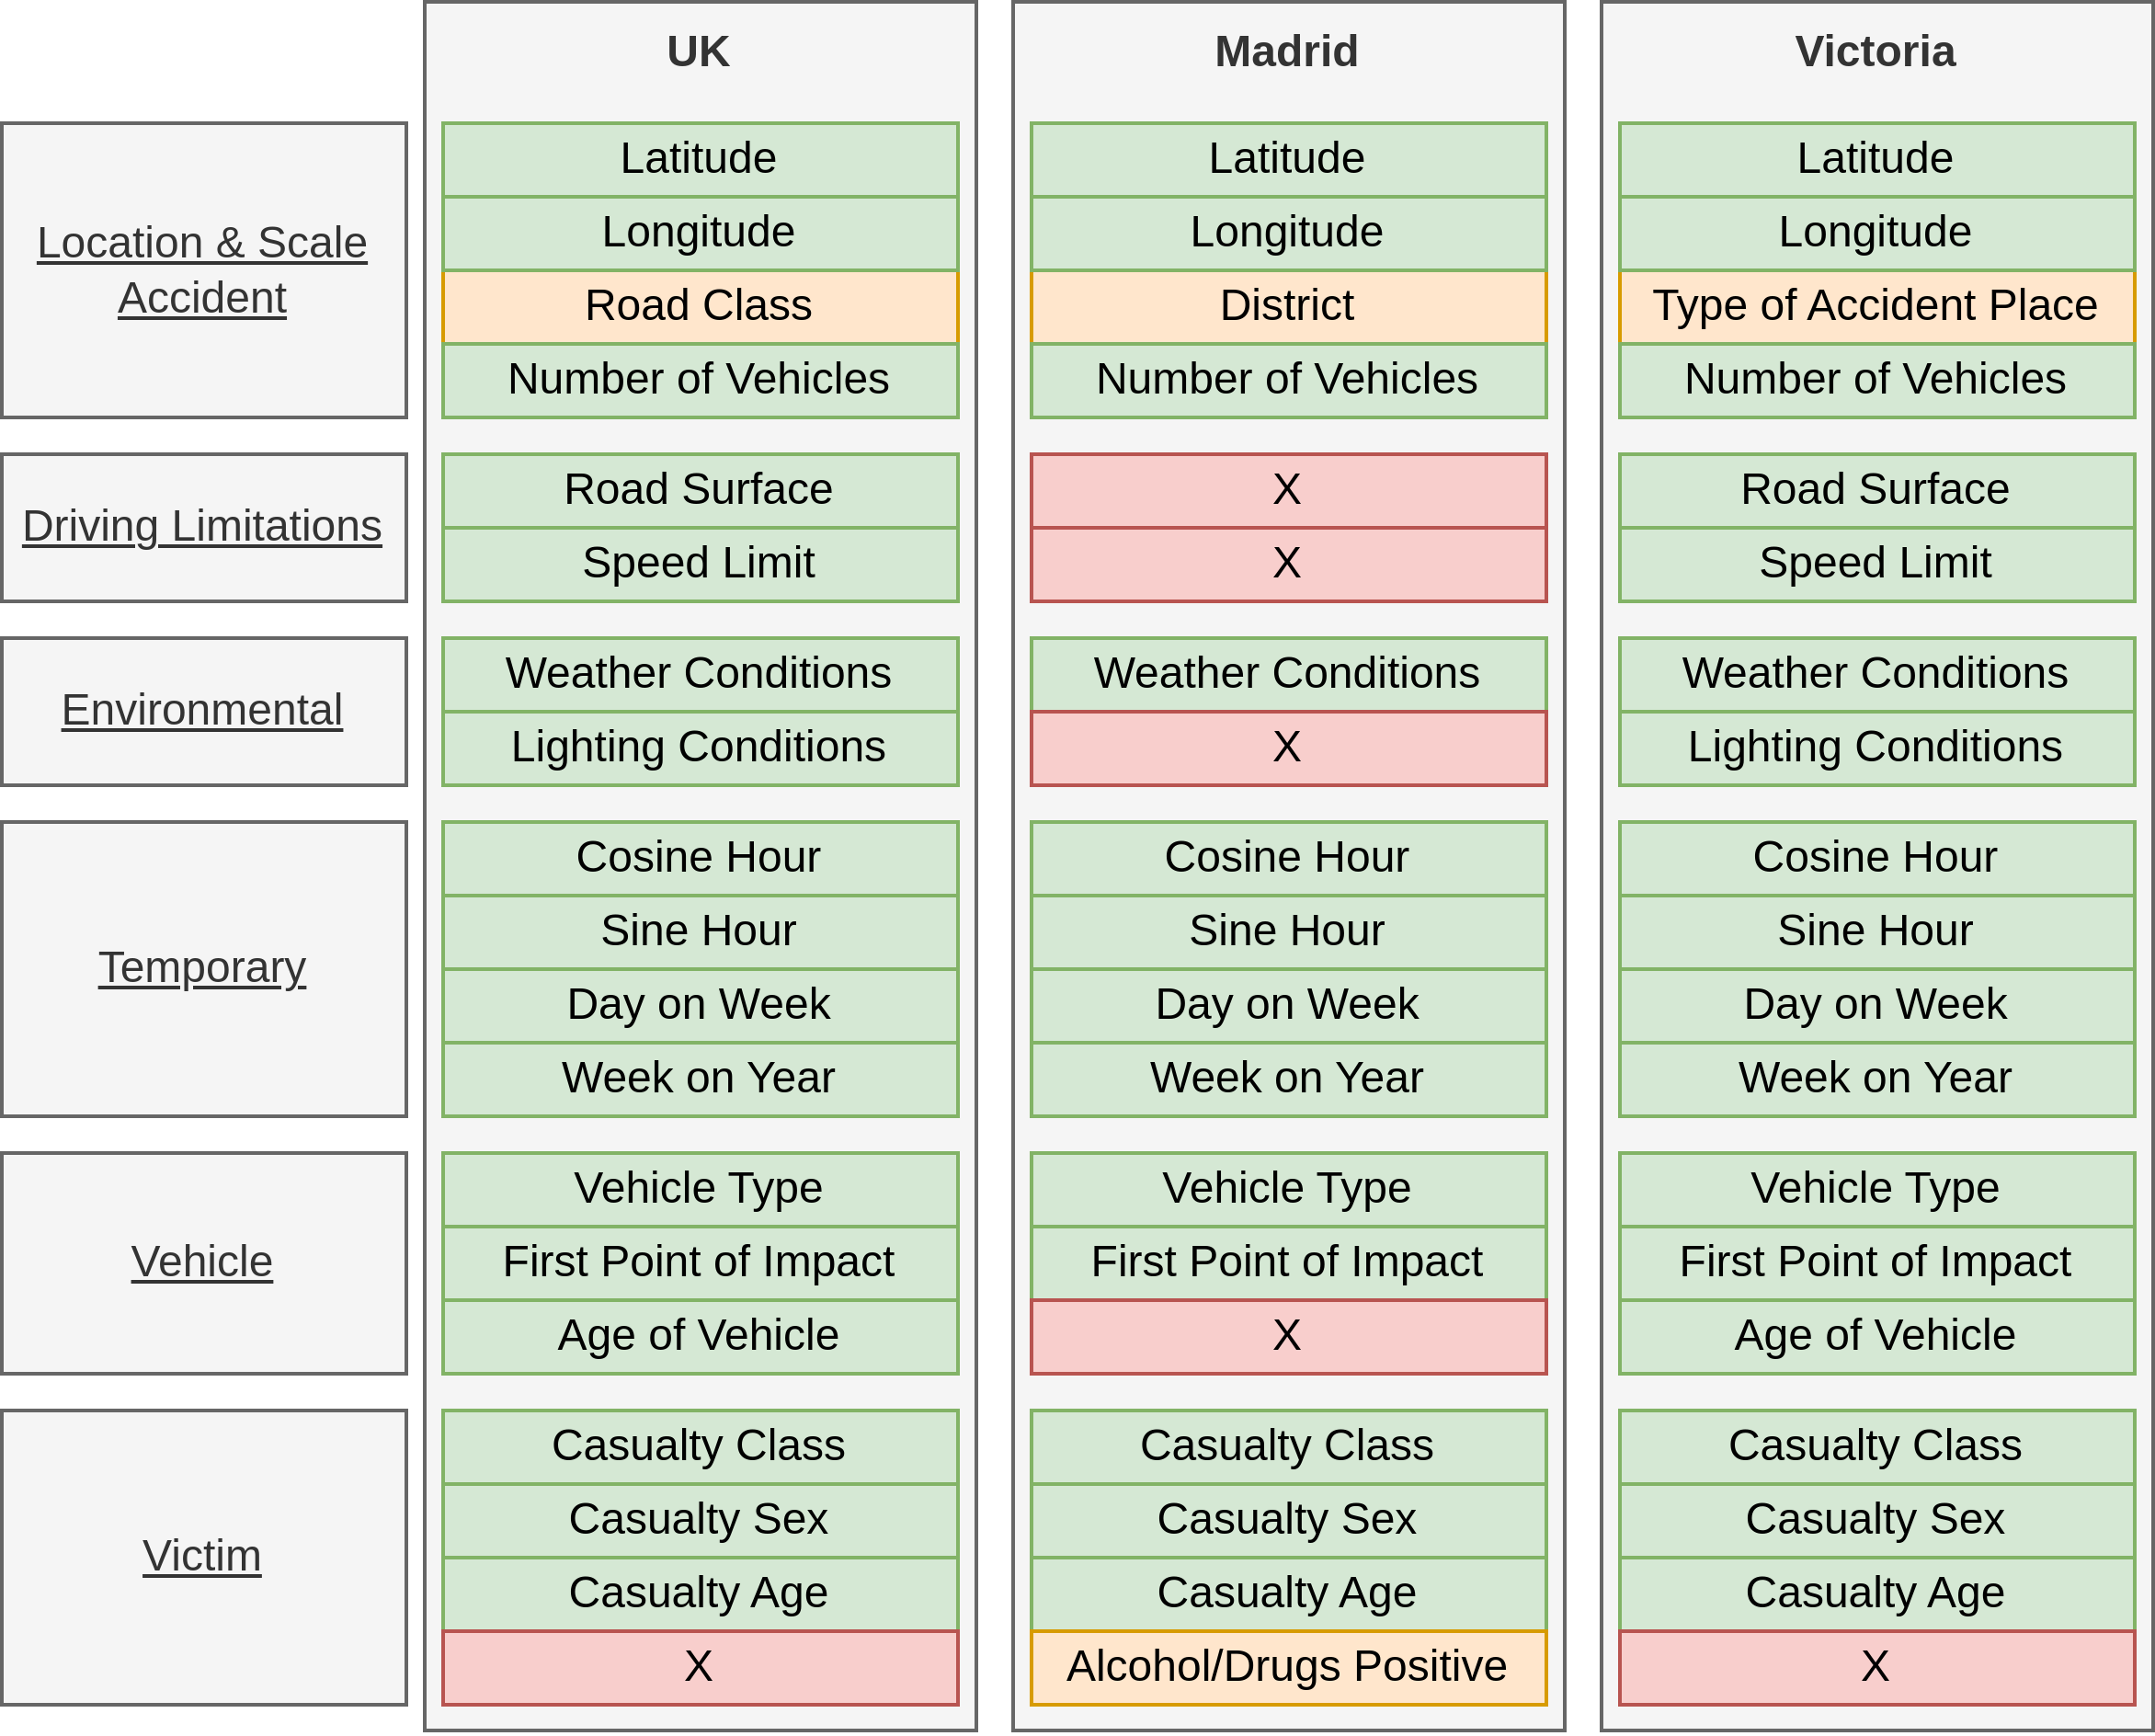
\includegraphics[width=12cm]{Figures/Dataset Comparative.png}
	\caption[Clasificación de variables para el modelo GTAAF]{Clasificación de variables para el modelo GTAAF. Los campos mostrados en amarillo representan características de la misma naturaleza pero difieren en la granularidad de los datos. Además, las características ausentes en comparación con otros conjuntos de datos están resaltadas en rojo}
	\label{FeaturesClassification}
\end{figure}

A continuación se detallarán aquellas partes comunes entre estos tres conjuntos de datos y las principales diferencias entre ellos.

\subsubsection*{Partes comunes entre los datos en base a la categorización}

Normalmente, en cualquier conjunto de datos que describa accidentes, existe información básica y de fácil obtención que suele ser común entre distintas regiones. Estas características suelen presentarse en forma de información espacial y temporal del accidente, como es la localización, las condiciones climáticas en el momento del suceso o la hora y fecha en la que se ha producido, como es el caso entre estos tres conjuntos de datos. Por otra parte, como es lógico, existe información básica que puede ser recogida rápidamente observando la escena del accidente, como es la localización, el número de vehículos implicados, las condiciones climáticas, la hora, el tipo de vehículo, el punto de impacto y las características del accidentado.


\subsubsection*{Principales diferencias entre los datos}

Cada una de las regiones ofrece información distinta en cada conjunto de datos. En este punto se analizarán las principales diferencias entre ellos en base a la categorización propuesta:

\textbf{Reino Unido}

En el caso de Reino Unido se observan ligeras diferencias respeto al resto de poblaciones. Como es el caso de la característica \textit{Road class} (para la categoría \textit{Localización y Escala del Accidente}), cuyo significado varía en comparación con el resto, y la ausencia de información sobre controles de estupefacientes a la víctima (categoría \textit{Víctima}). En el caso de \textit{Road Class}, este campo representa la clasificación de la carretera en la que se ha producido el accidente en base al tráfico que suele fluctuar sobre ella. Esta clasificación es responsabilidad de Gobierno de Reino Unido y se clasifican las vías en seis tipos diferentes: (1) Motorways: se trata de autopistas de alta velocidad que permiten el movimiento de vehículos entre los principales pueblos y ciudades. (2) A(M): se trata de carreteras principales que interconectan poblaciones y destinos de interés, estas vías pueden contener secciones transformadas en autovía. (3) A: carreteras importantes que conectan grandes densidades de tráfico entre zonas. Generalmente son las más anchas y directas, y son las de mayor importancia para el tráfico que contiene el área, estas carreteras pueden estar abiertas a distintos usuarios, como viandantes, ciclistas o caballos, aunque normalmente esto está restringido por las autoridades locales competentes. (4) Las carreteras B alimentan el tráfico entre las vías A y las carreteras más pequeñas de la red, siguen siendo de especial importancia para el tráfico, pero menos que las A. (5) Las carreteras tipo C son generalmente más pequeñas e interconectan las vías de tipo A y B. Normalmente unen urbanizaciones con el resto de carreteras de la red, son carreteras de menor importancia que las anteriores pero son de mayor relevancia respecto a las del siguiente tipo. (6) Carreteras no clasificadas, se tratan de vías destinadas al tráfico local, por su naturaleza la mayoría de las vías pertenecen a este tipo, generalmente tienen muy poca importancia y a nivel local \cite{UKDepartmentForTransportRoadClassification}.


\textbf{Madrid}

% \textcolor{orange}{\textbf{Luis: estoy llamando a las variables en inglés, pero así están en la tabla comparativa de arriba. Opiniones?}}

En el caso del conjunto de datos de Madrid, las diferencias respecto al resto de regiones se encuentra más acentuada. La información disponible es considerablemente menor en comparación con los datos de Reino Unido y de Victoria. Analizando la Figura \ref{FeaturesClassification} se puede observar que hay ciertas características que no están presentes, llegando a dejar incluso una categoría vacía (\textit{Limitaciones de Conducción}) al no disponer de información de este tipo. Por otra parte, tampoco se dispone de la información de \textit{Lighting Conditions} para la categoría \textit{Ambiental}, ni de \textit{Age of Vehicle}, en la categoría \textit{Vehículo}. No obstante, aún faltando esta información, el resto de características pueden ser asignadas a las categorías definidas, convirtiendo, por tanto, este dataset aplicable a este modelo.

Sin embargo, el conjunto de datos de Madrid ofrece información sobre si la víctima se encuentra bajo los efectos del alcohol o de sustancias estupefacientes. Al ser un dato que describe a la víctima del incidente, este será asignado a la categoría Victim.

Por otro lado, en la categoría \textit{Localización y Escala del Accidente} los datos de Madrid presentan una diferencia en lo que representa la característica \textit{District} respecto al resto de datasets. Este campo contempla el distrito dentro de Madrid en el que se ha producido el accidente, y es interpretado de forma numérica en función del orden de aparición de los distritos en los datos. Al ser una característica que ofrece información sobre la localización del accidente, será incluida en la categoría de \textit{Localización y Escala del Accidente}.

Como diferencia más notable sobre el conjunto de datos de Madrid es que \textbf{dispone de características para contemplar 5 categorías} respecto a las 6 de los otros dos conjuntos de datos.

\textbf{Victoria}

La información disponible en Victoria contempla un caso parecido al de los datos de Reino Unido, donde no se disponen de datos que describan si la víctima se encontraba bajo los efectos de estupefacientes o del alcohol, como es el caso de Madrid. Por lo que esta característica quedará vacía también en este conjunto de datos.

Respecto a la variable \textit{First Point of Impact}, este campo indica el tipo de colisión del vehículo, es decir, contra qué objeto ha impactado el vehículo, en comparación contra otros conjuntos de datos que indican también de qué parte del mismo ha impactado primero.

Por otra parte, la característica \textit{Type Of Accident Place}, ofrece información sobre el lugar del accidente, concretamente el lugar donde se ha producido, como autopista, parking, túnel, etc. por lo que irá asignada a la categoría \textit{Localización y Escala del Accidente}.



\subsection{Limpieza}
En la tabla \ref{DataDistribution} se expone el número total de registros de los datos originales y el número de muestras resultante tras haber aplicado la limpieza de estos datos para cada una de las poblaciones contempladas.

\begin{table}[H]
	\begin{center}
		\caption{Comparación de la distribución de datos tras el proceso de limpieza}
		\begin{tabular}{|c|c||c|c|}
			\hline
			\multicolumn{4}{ |c| }{\textbf{Distribución de Datos}} \\ \hline
			\multicolumn{4}{ |c| }{\textbf{Reino Unido}} \\ \hline
			
			\textbf{Región} & \textbf{Asistencia} & Original & Limpieza
			\\ \hline \hline
			
			\multirow{2}{*}{Southwark} &
			No   & 27.105  & 11.065 \\ &
			Sí  & 3.109   & 2.703 \\ \hline \hline
			\multirow{2}{*}{Manchester} &
			No  & 48.771   & 24.110 \\ &
			Sí  & 4.570    & 1.885 \\ \hline \hline
			\multirow{2}{*}{Birmingham} &
			No  & 108.723  & 64.147 \\ &
			Sí  & 11.187   & 6.191 \\ \hline \hline
			\multirow{2}{*}{Liverpool} &
			No  & 49.291  & 25.936 \\ &
			Sí  & 5.161   & 2.276 \\ \hline \hline
			\multirow{2}{*}{Sheffield} &
			No  & 43.579  & 25.622  \\ &
			Sí  & 5.887   & 2.703  \\ \hline \hline
			\multirow{2}{*}{Cornwall} &
			No  & 32.994 & 20.803 \\ &
			Sí  & 4.852 & 2.842 \\ \hline \hline
			
			\multicolumn{4}{ |c| }{\textbf{España}} \\ \hline
			
			\textbf{Región} & \textbf{Asistencia} & Original & Limpieza
			\\ \hline \hline
			
			\multirow{2}{*}{Madrid} &
			No  & 72.042  & 63.853   \\ &
			Sí & 1.472   & 1.305  \\ \hline \hline
			
			\multicolumn{4}{ |c| }{\textbf{Australia}} \\ \hline
			
			\textbf{Región} & \textbf{Asistencia} & Original & Limpieza
			\\ \hline \hline
			
			\multirow{2}{*}{Victoria} &
			No   & 7.064  & 5.556   \\ &
			Sí  & 7.059  & 6.024 \\ \hline \hline
			
		\end{tabular}

		\label{DataDistribution}
	\end{center}
\end{table}

% UK - Original
% - S: 266884
% - A: 34766
% - T: 301650
% UK - Cleaned
% - S: 197619
% - A: 18600
% - T: 216219
% Madrid
% - O: 60996
% - C: 43554
% Victoria
% - O: 14123
% - C: 11580


Como se puede observar, tras el proceso de limpieza, cada uno de los conjuntos de datos se ve afectado por una pérdida de registros significativa. Para Reino Unido, de un total de $301.650$ registros, se obtienen finalmente $216.219$, lo que supone un $28,3\%$ de pérdida de información respecto a la información inicial. En la ciudad de Madrid, $73,514$ registros en bruto iniciales acaban resultando en $65,158$ con información interpretable, conllevando un $11.38\%$ de pérdida de información. Por último, en el estado de Victoria, de un total de $14.123$ registros iniciales, resultan $11.580$ finales, asumiendo un $18\%$ de pérdida respecto a sus muestras iniciales.

\subsection{Discretización}

En esta sección se expone la discretización escogida para las variables de las tres regiones seleccionados para una mayor comprensión del tratamiento de las características en cada región.

\subsubsection*{Reino Unido}

La tabla \ref{UKFeaturesClassification} muestra la asignación de valores numéricos aplicada a los datos de las regiones de Reino Unido (Southwark, Manchester, Birmingham, Liverpool, Sheffield y Cornwall).

%%%%%%%%%%%%%%%%%%%%%%%%%%%%%%%%%%%%%%%%%%%%%%%%%%%%%%%%%%%%%%%%%%%%%%%%%%%%%%%%%
\begin{table}[H]
	\caption{Discretización propuesta de las variables para el conjunto de datos de Reino Unido}
	\scriptsize
	\begin{center}
		\begin{tabular}{|c|c|c|c|}
			\hline
			\textbf{Categoría} & \textbf{Característica} & \textbf{Valor} & \textbf{Descripción} \\ \hline 
			\hline
			
			\multirow{9}{*}{\textbf{\makecell{Localización y \\ Escala del accidente}}}
			& Latitud  & Número Real & Coordenada Este (OSGR) \\ \cline{2-4}
			& Longitud & Número Real & Coordenada Norte (OSGR) \\ \cline{2-4}
			& \multirow{6}{*} {Clase de Carretera}
			& 0 & Autopista \\ \cline{3-4}
			&& 1 & A(M) \\ \cline{3-4}
			&& 2 & A \\ \cline{3-4}
			&& 3 & B \\ \cline{3-4}
			&& 4 & C \\ \cline{3-4}
			&& 5 & No clasificada \\ \cline{2-4}
			& Número de Vehículos & 0-N & Dependiendo de los vehículos involucrados \\ \cline{2-4}
			
			\hline
			\hline
			
			\multirow{6}{*}{\textbf{\makecell{Limitaciones \\ de Conducción}}}
			& \multirow{5}{*} {Superficie de la Carretera}
			& 0 & Seca \\ \cline{3-4}
			&& 1 & Mojada / Húmeda \\ \cline{3-4}
			&& 2 & Nieve \\ \cline{3-4}
			&& 3 & Helada / Hielo \\ \cline{3-4}
			&& 4 & Inundación  \\ \cline{2-4}
			& Límite de Velocidad & 0-70 & Dependiendo del límite de velocidad (mph) \\ \cline{2-4}
			
			\hline
			\hline
			
			\multirow{13}{*}{\textbf{\makecell{Factores Ambientales}}} 
			& \multirow{8}{*} {Condiciones Meteorológicas}
			& 0 & Buen tiempo sin viento fuerte \\ \cline{3-4}
			&& 1 & Lluvia sin viento fuerte \\ \cline{3-4}
			&& 2 & Nieve sin viento fuerte \\ \cline{3-4}
			&& 3 & Buen tiempo con viento fuerte \\ \cline{3-4}
			&& 4 & Lluvia con viento fuerte \\ \cline{3-4}
			&& 5 & Nieve con viento fuerte \\ \cline{3-4}
			&& 6 & Niebla o neblina \\ \cline{3-4}
			&& 7 & Otro  \\ \cline{2-4}
			
			& \multirow{5}{*} {Condiciones de Iluminación}
			& 0 & Luz del día: luces de la calle presentes \\ \cline{3-4}
			&& 1 & Oscuridad: sin iluminación en la calle \\ \cline{3-4}
			&& 2 & Oscuridad: luces de la calle encendidas \\ \cline{3-4}
			&& 3 & Oscuridad: luces de la calle apagadas \\ \cline{3-4}
			&& 4 & Oscuridad: iluminación desconocida  \\ \cline{2-4}
			
			\hline
			\hline
			
			\multirow{4}{*}{\textbf{\makecell{Temporal}}} 
			& Hora Coseno & Número Real & Representación cosenoidal de la hora \\ \cline{2-4}
			& Hora Seno & Número Real & Representación senoidal de la hora \\ \cline{2-4}
			& Día de la Semana & 0-6 & Dependiendo del día de la semana \\ \cline{2-4}
			& Semana del Año & 0-52 & Dependiendo de la semana \\ \cline{2-4}
			
			\hline
			\hline
			
			\multirow{7}{*}{\textbf{Vehículo}}
			& Tipo de Vehículo & 0-17 & Dependiendo del peso del vehículo \\ \cline{2-4}
			& \multirow{5}{*} {Primer Punto de Impacto}
			& 0 & No impactó \\ \cline{3-4}
			&& 1 & Frente \\ \cline{3-4}
			&& 2 & Parte trasera \\ \cline{3-4}
			&& 3 & Lado contrario \\ \cline{3-4}
			&& 4 & Lado cercano \\ \cline{3-4}
			&& 5 & Desconocido (autoreportado) \\ \cline{2-4}
			& Edad del Vehículo  & 0-N & En orden de antigüedad del vehículo \\ \cline{2-4}
			
			\hline
			\hline
			
			\multirow{9}{*}{\textbf{Víctima}}
			& \multirow{3}{*} {Clase de Víctima}
			& 0 & Conductor/Motociclista \\ \cline{3-4}
			&& 1 & Pasajero \\ \cline{3-4}
			&& 2 & Peatón  \\ \cline{2-4}
			& \multirow{2}{*} {Sexo de la Víctima}
			& 0 & Masculino \\ \cline{3-4}
			&& 1 & Femenino  \\ \cline{2-4}
			& \multirow{4}{*} {Edad de la Víctima}
			& 0 & Menor de 18 años \\ \cline{3-4}
			&& 1 & Entre 18 y 25 años \\ \cline{3-4}
			&& 2 & Entre 25 y 65 años \\ \cline{3-4}
			&& 3 & Mayor de 65 años  \\ \cline{2-4}
			
			\hline
			\hline
		\end{tabular}
	\end{center}

	\label{UKFeaturesClassification}
\end{table}

%%%%%%%%%%%%%%%%%%%%%%%%%%%%%%%%%%%%%%%%%%%%%%%%%%%%%%%%%%%%%%%%%%%%%%%%%%%%%%%%%

\subsubsection*{Madrid}

La tabla \ref{MadridFeaturesClassification} muestra la asignación de valores aplicada a los datos de la región de Madrid. Como cuestión a considerar en este caso es que a la variable Distrito se le aplica un valor numérico en funcón del orden de aparición, sin que este represente ninguna importancia incremental.

%%%%%%%%%%%%%%%%%%%%%%%%%%%%%%%%%%%%%%%%%%%%%%%%%%%%%%%%%%%%%%%%%%%%%%%%%%%%%%%%%
\begin{table}[H]
	\caption{Discretización propuesta de las variables para el conjunto de datos de Madrid}
	\scriptsize
	\centering
	\begin{center}
		\begin{tabular}{|c|c|c|c|}
			\hline
			\textbf{Categoría} & \textbf{Característica} & \textbf{Valor} & \textbf{Descripción} \\ \hline 
			\hline
			
			\multirow{4}{*}{\textbf{\makecell{Localización \& \\ Escala del Accidente}}}
			& Latitud  & Número Real & Sistema de coordenadas cartesianas \\ \cline{2-4}
			& Longitud & Número Real & Sistema de coordenadas cartesianas \\ \cline{2-4}
			& Distrito  & 0-X & Número de distrito \\ \cline{2-4}
			& Número de Vehículos & 0-N & Dependiendo de los vehículos involucrados \\ \cline{2-4}
			\hline
			\hline
			
			\multirow{7}{*}{\textbf{\makecell{Factores Ambientales}}} 
			& \multirow{8}{*} {Condiciones Meteorológicas}
			& 0 & Despejado \\ \cline{3-4}
			&& 1 & Nublado \\ \cline{3-4}
			&& 2 & Lluvia ligera \\ \cline{3-4}
			&& 3 & Lluvia intensa \\ \cline{3-4}
			&& 4 & Granizo \\ \cline{3-4}
			&& 5 & Nevando \\ \cline{3-4}
			&& 6 & Desconocido \\ \cline{2-4}
			
			
			\hline
			\hline
			
			\multirow{4}{*}{\textbf{\makecell{Temporal}}} 
			& Hora Coseno & Número Real & Representación cosenoidal de la hora \\ \cline{2-4}
			& Hora Seno & Número Real & Representación senosoidal de la hora\\ \cline{2-4}
			& Día de la Semana & 0-6 & Dependiendo del día de la semana\\ \cline{2-4}
			& Semana del Año & 0-52 & Dependiendo de la semana \\ \cline{2-4}
			
			\hline
			\hline
			
			\multirow{15}{*}{\textbf{Vehículo}}
			& Tipo de Vehículo & 0-17 & Dependiendo del peso del vehículo \\ \cline{2-4}
			& \multirow{12}{*} {Primer Punto de Impacto}
			&  0 &  Colisión frontal - tamaño \\ \cline{3-4}
			&& 1 &  Colisión trasera \\ \cline{3-4}
			&& 2 &  Choque lateral \\ \cline{3-4}
			&& 3 &  Colisión contra obstáculo fijo \\ \cline{3-4}
			&& 4 &  Choque en cadena \\ \cline{3-4}
			&& 5 &  Atropello a peatón \\ \cline{3-4}
			&& 6 &  Colisión frontal \\ \cline{3-4}
			&& 7 &  Otro \\ \cline{3-4}
			&& 8 &  Abandonando la carretera \\ \cline{3-4}
			&& 9 &  Vuelco del vehículo \\ \cline{3-4}
			&& 10 &  Atropello a animal \\ \cline{3-4}
			&& 11 &  Caída \\ \cline{3-4}
			\hline
			\hline
			
			\multirow{9}{*}{\textbf{Víctima}}
			& \multirow{3}{*} {Clase de Víctima}
			& 0 & Conductor/Motociclista \\ \cline{3-4}
			&& 1 & Pasajero \\ \cline{3-4}
			&& 2 & Peatón  \\ \cline{2-4}
			& \multirow{2}{*} {Sexo de la Víctima}
			& 0 & Masculino \\ \cline{3-4}
			&& 1 & Femenino  \\ \cline{2-4}
			& \multirow{4}{*} {Edad de la Víctima}
			& 0 & Menor de 18 años \\ \cline{3-4}
			&& 1 & Entre 18 y 25 años \\ \cline{3-4}
			&& 2 & Entre 25 y 65 años \\ \cline{3-4}
			&& 3 & Mayor de 65 años  \\ \cline{2-4}
			& \multirow{2}{*} {Alcohol/Drogas Positivo}
			& 0 & No \\ \cline{3-4}
			&& 1 & Sí \\ \cline{3-4}
			\hline
			\hline
		\end{tabular}
	\end{center}

	\label{MadridFeaturesClassification}
\end{table}
%%%%%%%%%%%%%%%%%%%%%%%%%%%%%%%%%%%%%%%%%%%%%%%%%%%%%%%%%%%%%%%%%%%%%%%%%%%%%%%%%

\subsubsection*{Victoria}

La tabla \ref{VictoriaFeaturesClassification} muestra la discretización del valor las características que pueden tomar los registros de accidentes en el Estado de Victoria.

%%%%%%%%%%%%%%%%%%%%%%%%%%%%%%%%%%%%%%%%%%%%%%%%%%%%%%%%%%%%%%%%%%%%%%%%%%%%%%%%%
\begin{table}[H]
	\caption{Discretización propuesta de las variables para el conjunto de datos de Victoria}
	\scriptsize
	\begin{center}
		\begin{tabular}{|c|c|c|c|}
			\hline
			\textbf{Categoría} & \textbf{Característica} & \textbf{Valor} & \textbf{Descripción} \\ \hline 
			\hline
			
			\multirow{4}{*}{\textbf{\makecell{Localización \& \\ Escala del Accidente}}}
			& Latitud  & Número Real & Coordenada Este OSGR \\ \cline{2-4}
			& Longitud & Número Real & Coordenada Norte OSGR \\ \cline{2-4}
			& Clase de Carretera & 0-58 & En orden de aparición \\ \cline{2-4}
			& Número de Vehículos & 0-N & Dependiendo de los vehículos involucrados \\ \cline{2-4}
			
			\hline
			\hline
			
			
			\multirow{7}{*}{\textbf{\makecell{Limitaciones \\ de Conducción}}}
			& \multirow{6}{*} {Superficie de la Carretera}
			& 0 & Seco \\ \cline{3-4}
			&& 1 & Mojado / Húmedo \\ \cline{3-4}
			&& 2 & Fangosa \\ \cline{3-4}
			&& 3 & Nevada \\ \cline{3-4}
			&& 4 & Hielo  \\ \cline{3-4}
			&& 5 & Otro  \\ \cline{2-4}
			& Límite de Velocidad & 0-70 & Dependiendo del límite de velocidad (mph) \\ \cline{2-4}
			
			\hline
			\hline
			
			\multirow{15}{*}{\textbf{\makecell{Factores Ambientales}}} 
			& \multirow{8}{*} {Condiciones Meteorológicas}
			& 0 & Despejado \\ \cline{3-4}
			&& 1 & Lluvia \\ \cline{3-4}
			&& 2 & Nevando \\ \cline{3-4}
			&& 3 & Niebla \\ \cline{3-4}
			&& 4 & Humo en el ambiente \\ \cline{3-4}
			&& 5 & Polvo en el ambiente \\ \cline{3-4}
			&& 6 & Fuertes Vientos \\ \cline{3-4}
			&& 7 & Otro  \\ \cline{2-4}
			
			& \multirow{7}{*} {Condiciones de Iluminación}
			& 0 & Día \\ \cline{3-4}
			&& 1 & Amanecer \\ \cline{3-4}
			&& 2 & Oscuridad: luces de la calle encendidas \\ \cline{3-4}
			&& 3 & Oscuridad: luces de la calle apagadas \\ \cline{3-4}
			&& 4 & Oscuridad: sin luces de la calle \\ \cline{3-4}
			&& 5 & Oscuridad: iluminación desconocida \\ \cline{3-4}
			&& 6 & Otro  \\ \cline{2-4}
			
			\hline
			\hline
			
			\multirow{4}{*}{\textbf{\makecell{Temporal}}} 
			& Hora Coseno & Número Real & Representación cosenoidal de la hora\\ \cline{2-4}
			& Hora Seno & Número Real & Representación senosoidal de la hora\\ \cline{2-4}
			& Día de la Semana & 0-6 & Dependiendo del día de la semana \\ \cline{2-4}
			& Semana del Año & 0-52 & Dependiendo de la semana \\ \cline{2-4}
			
			\hline
			\hline
			
			\multirow{10}{*}{\textbf{Vehículo}}
			& Tipo de Vehículo & 0-17 & Dependiendo del peso del vehículo \\ \cline{2-4}
			& \multirow{8}{*} {Primer Punto de Impacto}
			& 0 & Colisión con vehículo \\ \cline{3-4}
			&& 1 & Atropello a peatón \\ \cline{3-4}
			&& 2 & Atropello a animal \\ \cline{3-4}
			&& 3 & Colisión contra obstáculo fijo \\ \cline{3-4}
			&& 3 & Colisión contra otro objeto \\ \cline{3-4}
			&& 5 & Vuelco del vehículo (sin colisión) \\ \cline{3-4}
			&& 6 & Caída desde vehículo en movimiento \\ \cline{3-4}
			&& 7 & Sin colisión y sin objeto golpeado) \\ \cline{2-4}
			& Edad del Vehículo  & 0-N & En orden de antigüedad del vehículo \\ \cline{2-4}
			
			\hline
			\hline
			
			\multirow{12}{*}{\textbf{Víctima}}
			& \multirow{6}{*} {Clase de Víctima}
			& 0 & Peatón \\ \cline{3-4}
			&& 1 & Conductor \\ \cline{3-4}
			&& 2 & Pasajero \\ \cline{3-4}
			&& 3 & Motociclista \\ \cline{3-4}
			&& 4 & Ciclista \\ \cline{3-4}
			&& 5 & Desconocido  \\ \cline{2-4}
			& \multirow{2}{*} {Sexo de la Víctima}
			& 0 & Masculino \\ \cline{3-4}
			&& 1 & Femenino  \\ \cline{2-4}
			& \multirow{4}{*} {Edad de la Víctima}
			& 0 & Menor de 18 años \\ \cline{3-4}
			&& 1 & Entre 18 y 25 años \\ \cline{3-4}
			&& 2 & Entre 25 y 65 años \\ \cline{3-4}
			&& 3 & Mayor de 65 años  \\ \cline{2-4}
			
			\hline
			\hline
		\end{tabular}
	\end{center}

	\label{VictoriaFeaturesClassification}
\end{table}
%%%%%%%%%%%%%%%%%%%%%%%%%%%%%%%%%%%%%%%%%%%%%%%%%%%%%%%%%%%%%%%%%%%%%%%%%%%%%%%%%


\subsection{Filtrado de áreas}


Para ilustrar los parámetros con los que se aplica el filtrado de áreas, se presenta la Tabla \ref{AreasInformation}, donde se muestra para cada población el número de áreas proyectadas resultante de la elección del tamaño de las ventanas en función de los valores \textit{X,Y}. La elección de estos tamaños variará función de la extensión y densidad de población, tomando valores de ventana más grandes en poblaciones más dispersas y tamaños más pequeños cuando la densidad de población es más alta. Los tamaños de ventana para cada población han sido escogidos mediante un procedimiento experimental, en el que se maximiza el rendimiento final de los modelos en base a la media total.

\begin{table}[H]
	\caption{Número de áreas resultante tras la definición de su tamaño para cada región}
	\begin{center}
		\begin{tabular}{|c|c||c|c|c||c|c|c}
			\hline
			\multicolumn{4}{ |c| }{\textbf{División de Áreas}} \\ \hline
			
			\multicolumn{4}{ |c| }{\textbf{Reino Unido}} \\ \hline
			\textbf{Región} & \textbf{Eje} & \textbf{Número de Áreas} & \textbf{Tamaño de Área}
			\\ \hline  \hline 
			
			\multirow{2}{*}{Southwark} &
			X  & 529  & 10 \\ &
			Y  & 487  & 20 \\ \hline \hline
			\multirow{2}{*}{Manchester} &
			X  & 791     & 14  \\ &
			Y  & 1.069    & 20  \\ \hline \hline
			\multirow{2}{*}{Birmingham} &
			X  & 3.519    & 12 \\ &
			Y  & 1.557    & 17 \\ \hline \hline
			\multirow{2}{*}{Liverpool} &
			X  & 2.107    & 12  \\ &
			Y  & 717     & 21  \\ \hline \hline
			\multirow{2}{*}{Sheffield} &
			X  & 1.896     & 12  \\ &
			Y  & 1.115     & 18 \\ \hline \hline
			\multirow{2}{*}{Cornwall} &
			X  & 10.090    & 15 \\ &
			Y  & 5.597    & 19 \\ \hline \hline
			
			\multicolumn{4}{ |c| }{\textbf{España}} \\ \hline
			\textbf{Región} & \textbf{Eje} & \textbf{Número de Áreas} & \textbf{Tamaño de Área}
			\\ \hline  \hline 
			
			\multirow{2}{*}{Madrid} &
			X  & 5.241  & 5 \\ &
			Y  & 4.444  & 7 \\ \hline \hline
			
			\multicolumn{4}{ |c| }{\textbf{Australia}} \\ \hline
			\textbf{Región} & \textbf{Eje} & \textbf{Número de Áreas} & \textbf{Tamaño de Área}
			\\ \hline  \hline 
			
			\multirow{2}{*}{Victoria} &
			X  & 4.931  & 145 \\ &
			Y  & 5.241  & 97 \\ \hline \hline
		\end{tabular}
	\end{center}

	\label{AreasInformation}
\end{table}

Una vez se establecen las dimensiones de las ventanas de tamaño $X,Y$ se aplica el filtrado para cada región, donde el número de muestras de la clase mayoritaria se ve considerablemente reducido respecto a la minoritaria, buscando obtener un conjunto de datos más balanceado. La Tabla \ref{DataDistributionFiltered} muestra el número de registros originales para cada población y el número de registros resultante tras aplicar el filtrado.

%%%%%%%%%%%%%%%%%%%%%%%%%%%%%%%%%%%%%%%%%%%%%%%%%%%%%%%%%%%%%%%%%%%%%%%%%%%%%%%%%
\begin{table}[H]
	\caption{Distribución de datos tras el proceso de filtrado para cada una de las regiones}
	\begin{center}
		\begin{tabular}{|c|c||c|c|}
			\hline
			\multicolumn{4}{ |c| }{\textbf{Distribución de Datos}} \\ \hline
			\multicolumn{4}{ |c| }{\textbf{Reino Unido}} \\ \hline
			
			\textbf{Región} & \textbf{Asistencia} & Limpieza & Filtrado
			\\ \hline \hline
			
			\multirow{2}{*}{Southwark} &
			No   & 11.065  & 4.251 \\ &
			Sí  & 2.703   & 1.256 \\ \hline \hline
			\multirow{2}{*}{Manchester} &
			No  & 24.110  & 4.548 \\ &
			Sí & 1.885   & 1.466 \\ \hline \hline
			\multirow{2}{*}{Birmingham} &
			No  & 64.147  & 4.092 \\ &
			Sí & 6.191   & 2.063 \\ \hline \hline
			\multirow{2}{*}{Liverpool} &
			No  & 25.936  & 3.640 \\ &
			Sí & 2.276   & 1.192 \\ \hline \hline
			\multirow{2}{*}{Sheffield} &
			No  & 25.622 & 2.060  \\ &
			Sí & 2.703  & 1.638  \\ \hline \hline
			\multirow{2}{*}{Cornwall} &
			No  & 20.803 & 2.191 \\ &
			Sí & 2.842  & 2.020 \\ \hline \hline
			
			\multicolumn{4}{ |c| }{\textbf{España}} \\ \hline
			
			\textbf{Región} & \textbf{Asistencia} & Limpieza & Filtrado
			\\ \hline \hline
			
			\multirow{2}{*}{Madrid} &
			No   & 63.840  & 2.601 \\ &
			Sí  & 1.305   & 1.286 \\ \hline \hline
			
			\multicolumn{4}{ |c| }{\textbf{Australia}} \\ \hline
			
			\textbf{Región} & \textbf{Asistencia} & Limpieza & Filtrado
			\\ \hline \hline
			
			\multirow{2}{*}{Victoria} &
			No   & 5.556  & 2.065  \\ &
			Sí  & 6.024  & 2.649  \\ \hline \hline
			
		\end{tabular}
	\end{center}

	\label{DataDistributionFiltered}
\end{table}

% UK
%     Original
%     - S: 171683
%     - A: 18600
% UK
%     Filtered
%     - S: 20782
%     - A: 9635
% Madrid
%     Cleaned: 43554
%     Filtered: 3887
% Victoria
%     Cleaned: 11580
%     Filtered: 4714

Una vez aplicado el filtrado de áreas los conjuntos de datos resultantes presentan un desbalanceo considerablemente menor. Para el dataset de Reino Unido se ha conseguido reducir, de media, una desproporción de las clases del $90,2\%$ y $9,8\%$ de los registros de las clases Sin Asistencia y Con Asistencia respectivamente hasta un  $53,6\%$ y $46,4\%$. Para la ciudad de Madrid se partía con un $98\%$ de accidentes Sin Asistencia y un $2\%$ de accidentes Con Asistencia, llegando una proporción final del  $67\%$ y $33\%$ respectivamente. Para la ciudad de Victoria se evoluciona desde un $48\%$ y $52\%$ a un $43,8\%$ $56,2\%$, por lo que sobre esta última, el proceso de remuestreo de clases afectará a la clase Sin Asistencia, siendo el único caso en el que esta es mayoritaria.

\subsection{Resampling}

En esta fase se seleccionan los datos de entrenamiento y de test. La distribución de esta división presenta un 80\% de los datos refinados como conjunto de entrenamiento, y 20\% restante como conjunto de validación o test. En la tabla \ref{Resampling} se muestra la distribución de estos datos junto con el número total de muestras de entrenamiento sobre el que se ha aplicado el proceso de aumentado de datos \textit{SMOTE-II}.

En la tabla \ref{Resampling} se muestran los datos resultantes tras haber aplicado el proceso de resampling mediante la generación de datos sintéticos de \textit{SMOTE-II}, conformando un dataset balanceado en el que se previene el riesgo de sesgo de datos por parte de los modelos.

%%%%%%%%%%%%%%%%%%%%%%%%%%%%%%%%%%%%%%%%%%%%%%%%%%%%%%%%%%%%%%%%%%%%%%%%%%%%%%%%%
\begin{table}[H]
	\caption[Distribución de datos para las ciudades seleccionadas. Modelo GTAAF]{Distribución de datos para las ciudades seleccionadas. Modelo GTAAF. La columna Asistencia representa si el accidente ha requerido de asistencia o no, las dos clases objetivo de este documento. La columna Filtrado indica el número de muestras disponibles tras el proceso de filtrado. La columna Entrenamiento representa el 80\% de las muestras de entrenamiento seleccionadas del total de los datos filtrados. La columna Test muestra el 20\% de los datos utilizados para la futura validación de los modelos. Finalmente \textit{Oversampled} engloba el número de muestra tras aplicar el aumentado de datos sobre el conjunto de entrenamiento de cada población mediante la técnica \textit{SMOTE-II} para la clase minoritaria}
	\begin{center}
		\begin{tabular}{|c|c||c|c|c|c|}
			\hline
			\multicolumn{6}{ |c| }{\textbf{Distribución de Datos}} \\ \hline
			\multicolumn{6}{ |c| }{\textbf{Reino Unido}} \\ \hline
			
			\textbf{Región} & \textbf{Asistencia} & Filtrado & Entrenamiento & Test & \textit{Oversampled}
			\\ \hline \hline
			
			\multirow{2}{*}{Southwark} &
			No   & 4.251  & 3.400 & 851 & 3.400  \\ &
			Sí  & 1.256  & 1.004 & 252 & 3.400 \\ \hline \hline
			\multirow{2}{*}{Manchester} &
			No   & 4.548  & 3.638 & 910 & 3.638 \\ &
			Sí  & 1.466  & 1.172 & 294 & 3.638 \\ \hline \hline
			\multirow{2}{*}{Birmingham} &
			No   & 4.092  & 3.273 & 819 & 3.273 \\ &
			Sí  & 2.063  & 1.650 & 413 & 3.273 \\ \hline \hline
			\multirow{2}{*}{Liverpool} &
			No   & 3.640 & 2.912 & 728 & 2.912  \\ &
			Sí  & 1.192 &   953 & 239 & 2.912 \\ \hline \hline
			\multirow{2}{*}{Sheffield} &
			No   & 2.060  & 1.648 & 412 & 1.648 \\ &
			Sí  & 1.638  & 1.310 & 328 & 1.648 \\ \hline \hline
			\multirow{2}{*}{Cornwall} &
			No   & 2.191  & 1.752 & 439 & 1.752 \\ &
			Sí  & 2.020  & 1.616 & 404 & 1.752 \\ \hline \hline
			
			\multicolumn{6}{ |c| }{\textbf{España}} \\ \hline
			\textbf{Región} & \textbf{Asistencia} & Filtrado & Entrenamiento & Test & \textit{Oversampled}
			\\ \hline \hline
			
			\multirow{2}{*}{Madrid} &
			No   & 2.601  & 2.080 & 521 & 2.080  \\ &
			Sí  & 1.286  & 1.028 & 258 & 2.080 \\ \hline \hline
			
			\multicolumn{6}{ |c| }{\textbf{Australia}} \\ \hline
			\textbf{Región} & \textbf{Asistencia} & Filtrado & Entrenamiento & Test & \textit{Oversampled}
			\\ \hline \hline
			
			\multirow{2}{*}{Victoria} &
			No   & 2.065 & 1.652 & 413 & 2.119  \\ &
			Sí  & 2.649 & 2.119 & 530 & 2.119 \\ \hline \hline
		\end{tabular}
	\end{center}

	\label{Resampling}
\end{table}
%%%%%%%%%%%%%%%%%%%%%%%%%%%%%%%%%%%%%%%%%%%%%%%%%%%%%%%%%%%%%%%%%%%%%%%%%%%%%%%%%


\subsection{Normalización}


En la Tabla \ref{FeaturesNormalizationExample} se muestra un ejemplo de la aplicación de la normalización de datos en base a la técnica \textit{Z-Score}, donde en la primera columna se observan los datos discretizados, mientras que la segunda columna contiene los valores de estas características normalizados.

\begin{table}[H]
	\caption{Ejemplo de muestra original y muestra normalizada}
	\begin{center}
		\begin{tabular}{|c|c||c|c|}
			\hline
			
			\textbf{Categoría} & \textbf{Característica} & \textbf{Valor Discretizado} & \textbf{Valor Normalizado}
			\\ \hline \hline
			
			\multirow{4}{*}{\textbf{\makecell{Location \& \\ Scale Accident}}} &
			Easting & 2511861.414 & -0.527831\\
			& Northing & 2374246.840 &  -1.057103\\
			& 1st Road Class & 3 &  -0.167530\\
			& Number of Vehicles & 2 &  -0.322890\\ \hline \hline
			\multirow{2}{*}{\textbf{\makecell{Driving \\ Limitations}}} &
			Road Surface & 1 & -0.265693 \\
			& Speed Limit & 80 &  -0.005659 \\ \hline \hline
			\multirow{2}{*}{\textbf{Environmental}} &
			Weather Conditions & 1 & -0.259213 \\
			& Lighting Conditions & 1 &  -0.479225\\ \hline \hline
			\multirow{4}{*}{\textbf{Temporary}} &
			Cosine Hour & -0.9659258 & -1.055298 \\
			& Sine Hour & 0.258819 &  0.840276 \\
			& Day on Week & 4 &  -0.055442 \\
			& Week on Year & 52 &  0.844870 \\ \hline \hline
			\multirow{3}{*}{\textbf{Vehicle}} &
			Vehicle Type & 1 & -0.294511 \\
			& First Point of Impact & 1 &  -0.363744 \\
			& Age of Vehicle & 1992 &  -0.062428 \\ \hline \hline
			\multirow{3}{*}{\textbf{Victim}} &
			Casualty Class & 3 & 0.724902 \\
			& Casualty Sex & 0 &  -0.858795 \\
			& Casualty Age & 1 &  -2.062940 \\ \hline \hline
		\end{tabular}
	\end{center}

	\label{FeaturesNormalizationExample}
\end{table}



Una vez se disponen de los datos normalizados, estos ya son comparables y por tanto pueden ser utilizados para el entrenamiento de cualquier modelo que acepte valores numéricos como entrada.


\subsection{Algoritmo Genético}


En la tabla \ref{GAHyperparametersSetup} se muestran los hiperparámetros del algoritmo genético utilizados para optimizar el algoritmo \textit{XGBoost}. Durante cada una de las generaciones, el límite máximo en la población es de 50 individuos (fila \textit{Población}). Estos individuos en cada generación son evaluados mediante la función heurística a optimizar, la métrica \textit{F1-Score} resultante del algoritmo \textit{XGBoost}, entrenado con dicha configuración de hiperparámetros, sobre el conjunto de test accidentes, es decir, en los accidentes no vistos durante el entrenamiento (fila \textit{Función Heurística}). Una vez son evaluados, aquellos 10 mejores individuos son seleccionados para intercambiar su información, los padres que darán lugar a 10 nuevos individuos de cara a la próxima generación (fila \textit{Padres Emparejados}). La mezcla de información entre padres se realiza mediante una estrategia de cruce mixta (fila \textit{Índice de Cruzamiento}), es decir, para cada par de padres se asigna un índice aleatorio en sobre el que se dividirán ambos individuos para luego combinar esta información en el descendiente resultante mediante cruce por punto aleatorio de las soluciones. Una vez se han dado lugar a los 10 nuevos individuos, el valor de cada una de las componentes que los conforman pueden ser modificados con una probabilidad del 40\% (fila \textit{Probabilidad de Mutación)}. Este proceso será repetido a lo largo de todas las 50 generaciones (fila \textit{Generaciones}).


%%%%%%%%%%%%%%%%%%%%%%%%%%%%%%%%%%%%%%%%%%%%%%%%%%%%%%%%%%%%%%%%%%%%%%%%%%%%%%%%%
\begin{table}[H]
	\caption{Configuración de hiperparámetros del algoritmo genético para el modelo GTAAF}
	\centering
	\begin{tabular}{|c|c|}
		\hline
		\textbf{Hiperparámetro} & \textbf{Valor} \\ \hline
		\hline
		Población     & 50 \\ \hline
		Padres Emparejados & 10 \\ \hline
		Generaciones    & 50 \\ \hline
		Índice de Cruzamiento & Aleatorio \\ \hline
		Probabilidad de Mutación & 0.4 \\ \hline
		Función Heurística & Puntuación \textit{F1-Score} del \textit{XGBoost} \\ \hline \hline
	\end{tabular}

	\label{GAHyperparametersSetup}
\end{table}
%%%%%%%%%%%%%%%%%%%%%%%%%%%%%%%%%%%%%%%%%%%%%%%%%%%%%%%%%%%%%%%%%%%%%%%%%%%%%%%%%

La Tabla \ref{MutationXGBoostParams} muestra las variaciones en los valores máximos y mínimos permitidos para cada variable a optimizar mediante el algoritmo genético. La fila \textit{Inicial} de cada hiperparámetro muestra el rango de valores que cada individuo puede tomar cuando es inicializado. En la fila \textit{Mutación} se observan, para cada hiperparámetro, los valores límites permitidos sobre los que los componentes de un sujeto pueden modificarse en el proceso de mutación, siempre y cuando dicho componente haya sido seleccionado para mutarse.

%%%%%%%%%%%%%%%%%%%%%%%%%%%%%%%%%%%%%%%%%%%%%%%%%%%%%%%%%%%%%%%%%%%%%%%%%%%%%%%%%
\begin{table}[H]
	\caption{Límites de inicialización y mutación de los hiperparámetros del algoritmo genético del modelo GTAAF}
	\begin{center}
		\begin{tabular}{|c|c||c|c|}
			\hline
			\textbf{Hiperparámetro} & \textbf{Límite} & \textbf{Mínimo} & \textbf{Máximo}
			\\ \hline \hline
			
			\multirow{2}{*}{ETA} &
			Inicial  & 0.01  & 1  \\ &
			Mutación & -0.2  & 0.2 \\ \hline \hline
			\multirow{2}{*}{Profundidad Máxima} &
			Inicial  & 1   & 25  \\ &
			Mutación & -3  & 3 \\ \hline \hline
			\multirow{2}{*}{Peso Mínimo de Hijos} &
			Inicial  & 0.01   & 20  \\ &
			Mutación & -4  & 4 \\ \hline \hline
		\end{tabular}
	\end{center}

	\label{MutationXGBoostParams}
\end{table}
%%%%%%%%%%%%%%%%%%%%%%%%%%%%%%%%%%%%%%%%%%%%%%%%%%%%%%%%%%%%%%%%%%%%%%%%%%%%%%%%%

La configuración de estos parámetros, tanto los iniciales como los de mutación, se han escogido en base a resultados experimentales, donde se ha priorizado la maximización de la métrica \textit{F1-Score} entre distintos experimentos.

En la Tabla \ref{ResultingHyperparamsXGBoost} se pueden observar los hiperparámetros óptimos resultantes de la ejecución del algoritmo genético, donde para cada región se observa la tasa de aprendizaje de los árboles (\textit{ETA}), la profundidad máxima de los árboles y el peso mínimo de los hijos para decidir la separación a través del nivel de los árboles.

%%%%%%%%%%%%%%%%%%%%%%%%%%%%%%%%%%%%%%%%%%%%%%%%%%%%%%%%%%%%%%%%%%%%%%%%%%%%%%%%%
\begin{table}[H]
	\caption{Hiperparámetros resultantes del \textit{XGBoost} después de ejecutar el algoritmo genético del modelo GTAAF}
	\begin{center}
		\begin{tabular}{|c||c|c|c|}
			\hline
			\multicolumn{4}{ |c| }{\textbf{Valores Resultantes del Algoritmo Genético}} \\ \hline
			
			\multicolumn{4}{ |c| }{\textbf{Reino Unido}} \\ \hline
			
			\textbf{Región} & \textbf{ETA} & \textbf{Profundidad Máxima} & \textbf{Peso Mínimo de Hijos}
			\\ \hline \hline
			
			\multirow{1}{*}{Southwark} &
			0.62  & 13 & 0.01 \\ \hline
			\multirow{1}{*}{Manchester} &
			0.01  & 1  & 0.01  \\ \hline
			\multirow{1}{*}{Birmingham} &
			0.43  & 17  & 0.01 \\ \hline
			\multirow{1}{*}{Liverpool} &
			0.83  & 12  & 0.01  \\ \hline
			\multirow{1}{*}{Sheffield} &
			0.59  & 20  & 0.61 \\ \hline
			\multirow{1}{*}{Cornwall} &
			0.85  & 17 & 0.01 \\ \hline \hline
			
			\multicolumn{4}{ |c| }{\textbf{España}} \\ \hline
			\textbf{Región} & \textbf{ETA} & \textbf{Profundidad Máxima} & \textbf{Peso Mínimo de Hijos}
			\\ \hline \hline
			
			\multirow{1}{*}{Madrid} &
			0.01  & 1 & 0.01
			\\ \hline \hline
			
			\multicolumn{4}{ |c| }{\textbf{Australia}} \\ \hline
			\textbf{Región} & \textbf{ETA} & \textbf{Profundidad Máxima} & \textbf{Peso Mínimo de Hijos}
			\\ \hline \hline
			\multirow{1}{*}{Victoria} &
			0.6  & 25 & 0.01 
			\\ \hline \hline
			
		\end{tabular}
	\end{center}

	\label{ResultingHyperparamsXGBoost}
\end{table}
%%%%%%%%%%%%%%%%%%%%%%%%%%%%%%%%%%%%%%%%%%%%%%%%%%%%%%%%%%%%%%%%%%%%%%%%%%%%%%%%%

\subsection{Construcción de matrices}

Una vez obtenidos los pesos de las características para cada población mediante el algoritmo \textit{XGBoost} optimizado con hiperparámetros, los registros tabulares de cada una de las poblaciones son convertidos a matrices, siendo estas interpretables por el modelo convolucional propuesto GTAAF.

Como los conjuntos de datos utilizados en esta tesis disponen de distintas características, el número de categorías disponibles varía entre ellos, y por tanto la dimensionalidad de las matrices resultantes es distinta entre sí. En el caso del conjunto de datos de Madrid se disponen de 5 de las 6 categorías propuestas, al no disponer de información sobre las limitaciones de la conducción. Por lo que las matrices de entrada para el modelo convolucional serán de 5x4 mientras que para los datos de Reino Unido y Victoria serán de 6x4 al disponer de características que pueden ser englobadas en las 6 categorías. 

% \textcolor{red}{\textbf{Luis: Inquietud} aquí no sé qué más poner.}

\section{Evaluación del modelo GTAAF}

En esta sección se presentarán los resultados del modelo GTAAF tras su ejecución sobre las ocho poblaciones propuestas en esta tesis. Para evaluar la generalización del modelo en distintos contextos, los resultados del modelo convolucional se compararán con otros seis modelos del estado del arte (\textit{SVC, Naive Bayes, Random Forest, KNN, Regresión Logística y MLP}). Los resultados se exponen para cada conjunto de datos, donde se comenzará con Madrid, en segundo lugar se analizarán los resultados de Victoria y en último lugar las seis poblaciones de Reino Unido, cada una con una densidad distinta de habitantes. Los dos primeros casos (Madrid y Australia) presentan condiciones de densidad de población opuestas, alta y baja respectivamente.

\subsection{Comparativas}
\subsubsection*{Madrid}

Este primer caso presenta una situación de alta densidad sobre la ciudad de Madrid. En la figura \ref{MadridAccidentsMap} se muestra la distribución de los accidentes original y la distribución resultante tras aplicar el filtrado por áreas, aquellos accidentes Sin Asistencia se encuentran representados en verde, mientras que los accidentes Con Asistencia encuentran representados en rojo. Como puede observarse en la figura \ref{MadridAccidentsMap:Original}, la concentración de los accidentes se ve distribuida principalmente por aquellas zonas más próximas al núcleo urbano de Madrid, contando además con una amplia concentración en aquellas carreteras que pertenecen a las principales arterias de comunicación de la ciudad. La figura  \ref{MadridAccidentsMap:Filtered} muestra la distribución de accidentes resultante tras haber aplicado el proceso de filtrado de áreas. Este proceso de reducción de datos permite una simplificación de la información sin que esto represente una pérdida en sí misma, ya que se busca equilibrar el número de accidentes Con Asistencia y Sin Asistencia, manteniendo únicamente la información imprescindible para ello.

\begin{figure}[H]
	\centering
	\subfloat[][Mapa de los accidentes originales de Madrid]{
		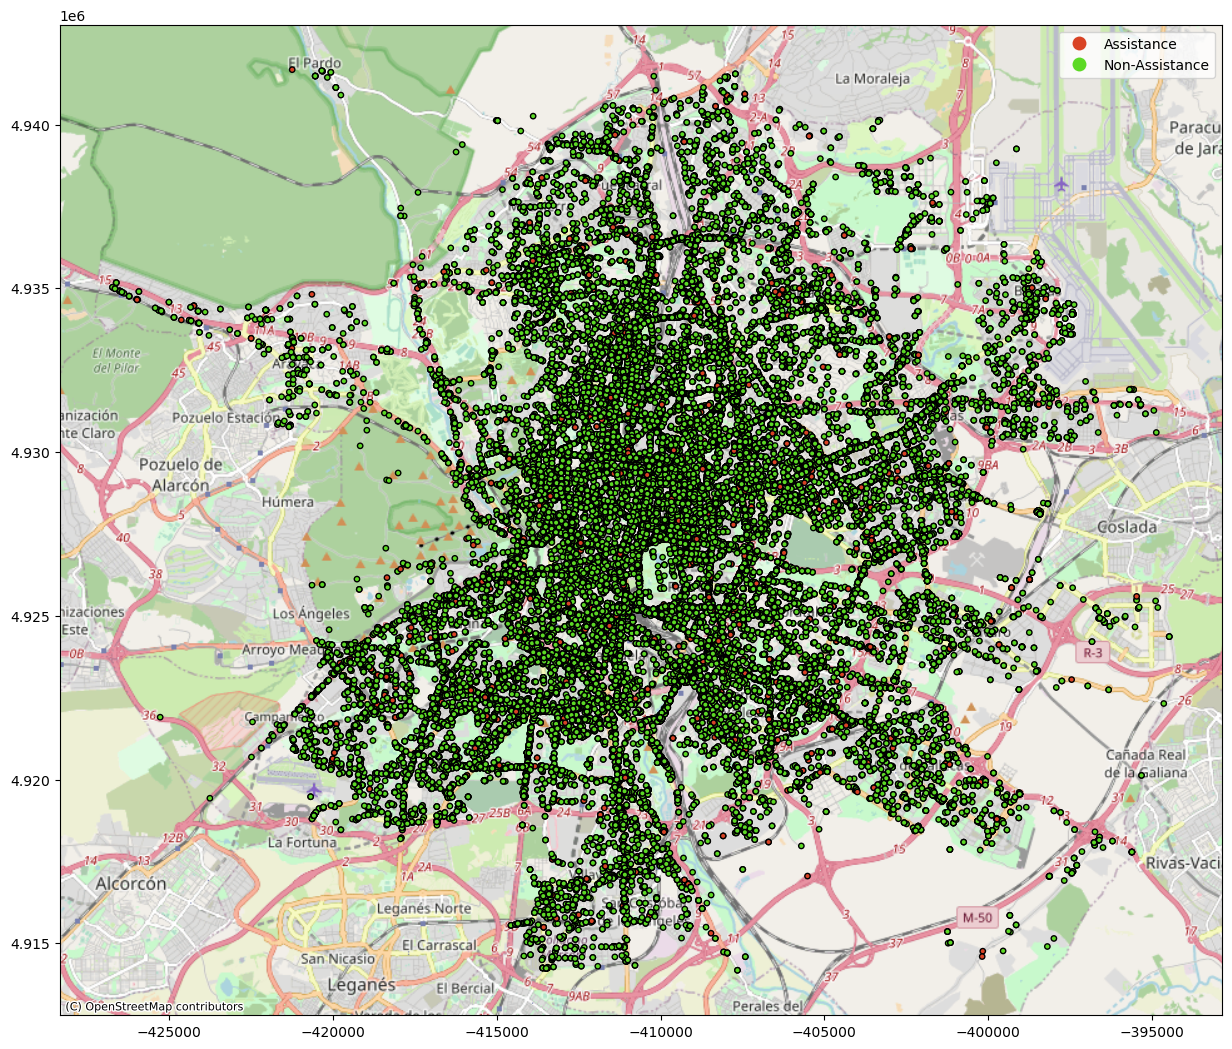
\includegraphics[width=90mm]{Figures/Madrid/original_OpenStreetMap.Mapnik.png}
		\label{MadridAccidentsMap:Original}
	}\\
	\subfloat[][Mapa de los accidentes filtrados de Madrid]{
		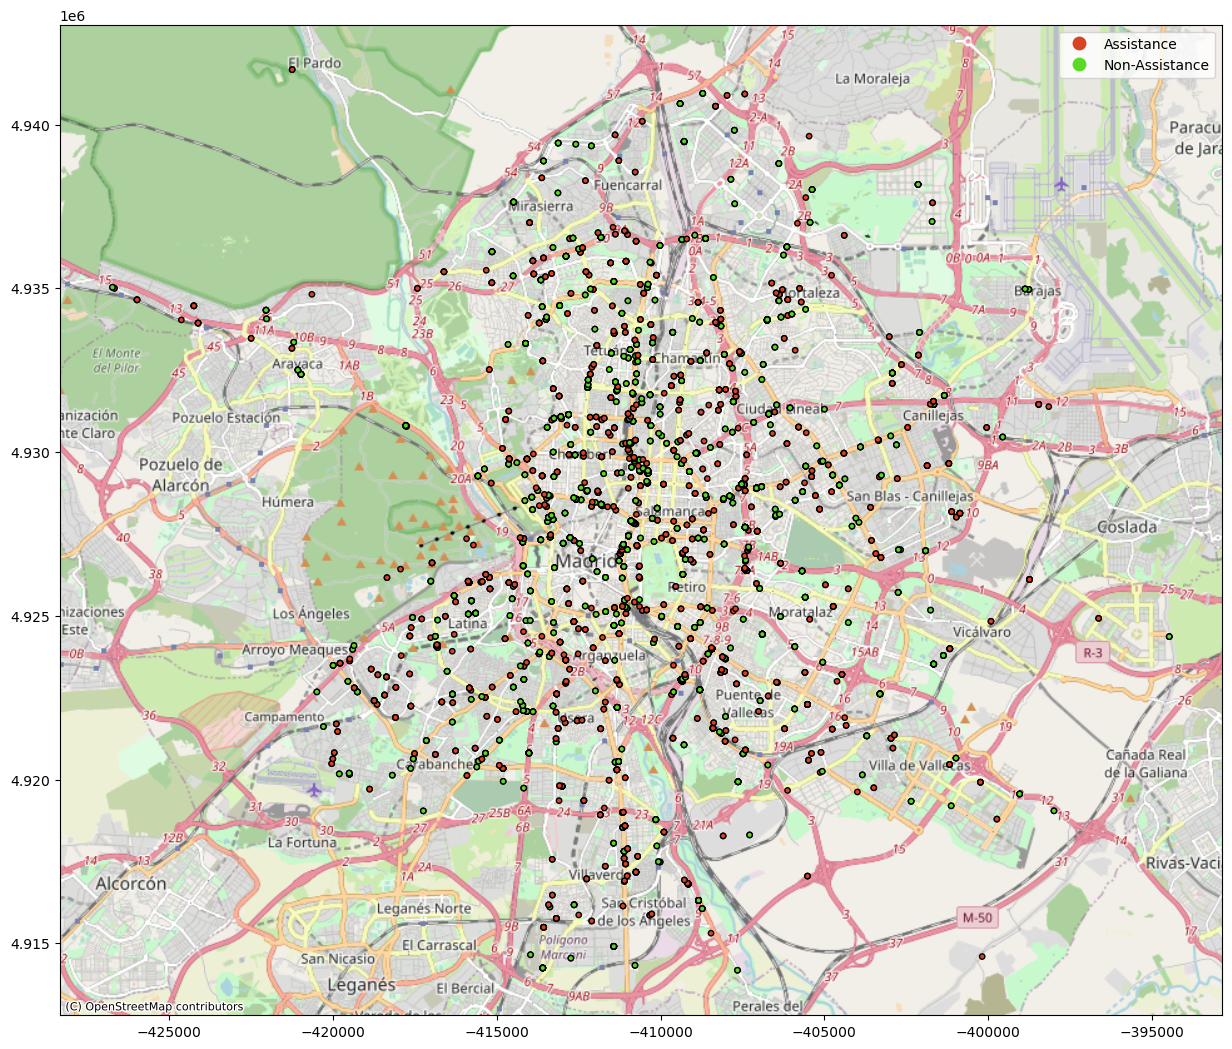
\includegraphics[width=90mm]{Figures/Madrid/filtered_OpenStreetMap.Mapnik.png}
		\label{MadridAccidentsMap:Filtered}
	}\\
	\caption{Mapa de accidentes de Madrid, original y filtrado}
	\label{MadridAccidentsMap}
\end{figure}

En la Figura \ref{MadridLossFunction} se muestra la evolución de la función a optimizar (\textit{F1-Score}) a lo largo de las 50 épocas para las que se ha entrenado el modelo GTAAF en la ciudad de Madrid. Se observa cómo el \textit{F1-Score} para el conjunto de entrenamiento sufre una evolución importante durante las diez primeras épocas, después de las cuales sigue aumentando en menor medida. Por otra parte, la métrica sobre el conjunto de validación sufre una evolución más lenta, hasta aproximadamente la época 30 no se ve una clara evolución en la generalización del modelo sobre datos que nunca ha visto.


\begin{figure}[h]
	\centering
	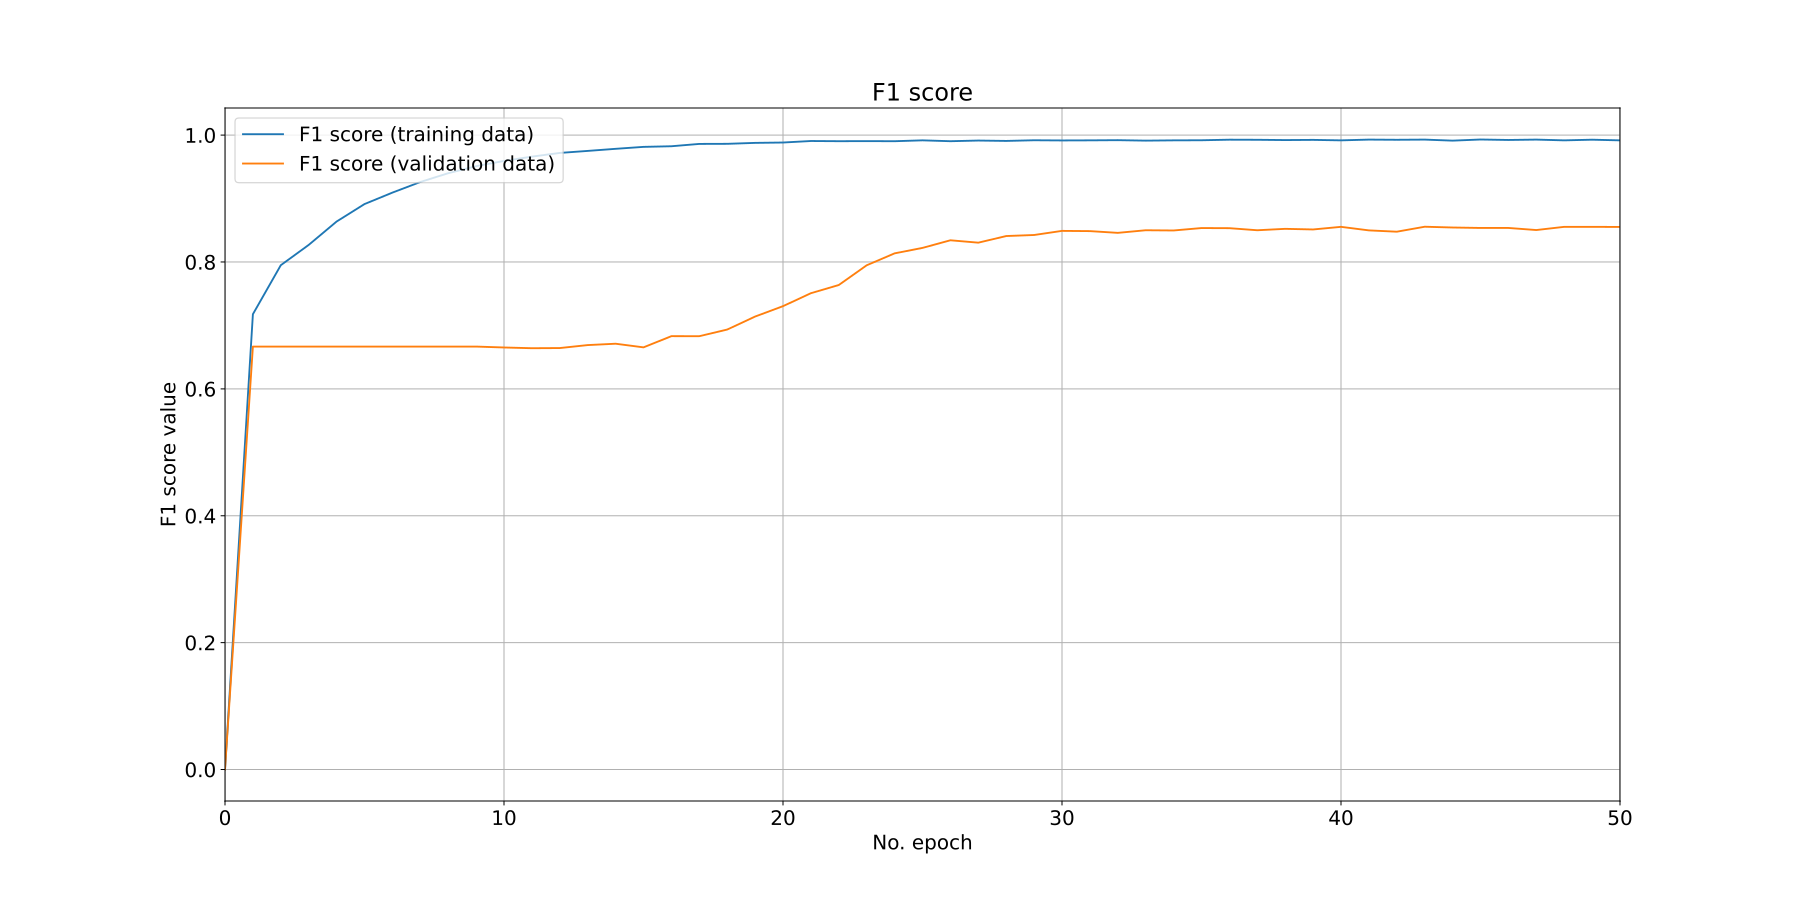
\includegraphics[width=14cm]{Figures/Madrid/madrid_convolution_2d_f1_score_2023-12-03-12 54 29.png}
	\caption{Evolución de \textit{F1-Score} del modelo GTAAF en Madrid}
	\label{MadridLossFunction}
\end{figure}

En la tabla \ref{SpainMetrics} se observan los resultados de la métrica \textit{F1-Score} de la predicción de la gravedad de los accidentes de cada uno de los modelos sobre el conjunto de test de la ciudad de Madrid. Como se puede comprobar, el valor más alto lo ofrece el nuevo modelo GTAAF, llegando a mejorar en un 3,9\% al siguiente mejor modelo, el \textit{SVC} sobre los accidentes Sin Asistencia, mientras que la mejora sobre los accidentes Con Asistencia se presenta en un 5,7\% sobre el siguiente modelo que mejor métricas ofrece, el \textit{SVC}. Con estos resultados se puede interpretar que el nuevo modelo GTAAF propuesto es capaz de generalizar mejor en la predicción de la gravedad de nuevos accidentes que no ha visto previamente sobre la ciudad de Madrid.

%%%%%%%%%%%%%%%%%%%%%%%%%%%%%%%%%%%%%%%%%%%%%%%%%%%%%%%%%%%%%%%%%%%%%%%%%%%%%%%%%
\begin{table}[H]
	\caption{\textit{F1-Score} por modelo y clase de accidente en Madrid (España)}
	\begin{center}
		\begin{tabular}{|c|c||c|c|c|c|c|c|}
			\hline
			\multicolumn{2}{ |c|| }{} &
			\multicolumn{1}{ |c| }{\textbf{\textit{F1-Score} España}} \\ \hline
			
			\textbf{Modelo} & \textbf{Asistencia} & Madrid
			\\ \hline \hline
			
			\multirow{2}{*}{NB} &
			No &  0.729 \\ &
			Sí & 0.621 \\ \hline \hline
			\multirow{2}{*}{SVC} &
			No & 0.862 \\ &
			Sí &  0.748 \\ \hline \hline
			\multirow{2}{*}{KNN} &
			No  & 0.739 \\ &
			Sí & 0.634 \\ \hline \hline
			\multirow{2}{*}{RF} &
			No & 0.744 \\ &
			Sí & 0.643  \\ \hline \hline
			\multirow{2}{*}{LR} &
			No &  0.750 \\ &
			Sí & 0.623 \\ \hline \hline
			\multirow{2}{*}{MLP} &
			No & 0.856 \\ &
			Sí & 0.724  \\ \hline \hline
			\multirow{2}{*}{\textbf{GTAAF}} &
			\textbf{No} & \textbf{0.894} \\ &
			\textbf{Sí} & \textbf{0.798} \\ \hline \hline
		\end{tabular}
	\end{center}

	\label{SpainMetrics}
\end{table}
%%%%%%%%%%%%%%%%%%%%%%%%%%%%%%%%%%%%%%%%%%%%%%%%%%%%%%%%%%%%%%%%%%%%%%%%%%%%%%%%%

\subsubsection*{Victoria}

En el segundo caso, tenemos una región dispersa, el estado de Victoria (Australia). Victoria, estado en Australia, abarca una región muy extensa y con gran diversidad, desde regiones desérticas hasta ciudades multitudinarias como Melbourne, situada a lo largo de la costa sureste. En la figura \ref{VictoriaAccidentsMap} se muestra la distribución de accidentes sobre la población de Victoria, aquellos Sin Asistencia se encuentran marcados en verde mientras que aquellos tipo Con Asistencia se encuentran representados en rojo. Como se puede observar en la figura \ref{VictoriaAccidentsMap:Original} gran parte de la concentración de los accidentes se encuentra sobre la ciudad de Melbourne y sus núcleos urbanos próximos (como Ballarat al oeste, Shepparton al norte o Traralgon al este), al igual que en las carreteras que conectan estas poblaciones. Al ser un estado extenso, el filtrado de áreas es más amplio, lo que resulta una variante respecto a ciudades de mayor concentración. En la Figura \ref{VictoriaAccidentsMap:Filtered} se observa la distribución de accidentes resultante tras aplicar el proceso de filtrado, donde aquellas zonas que presentan más accidentes Con Asistencia son en las grandes poblaciones y en las interconexiones entre estas.


\begin{figure}[H]
	\centering
	\subfloat[][Mapa de los accidentes originales de Victoria]{
		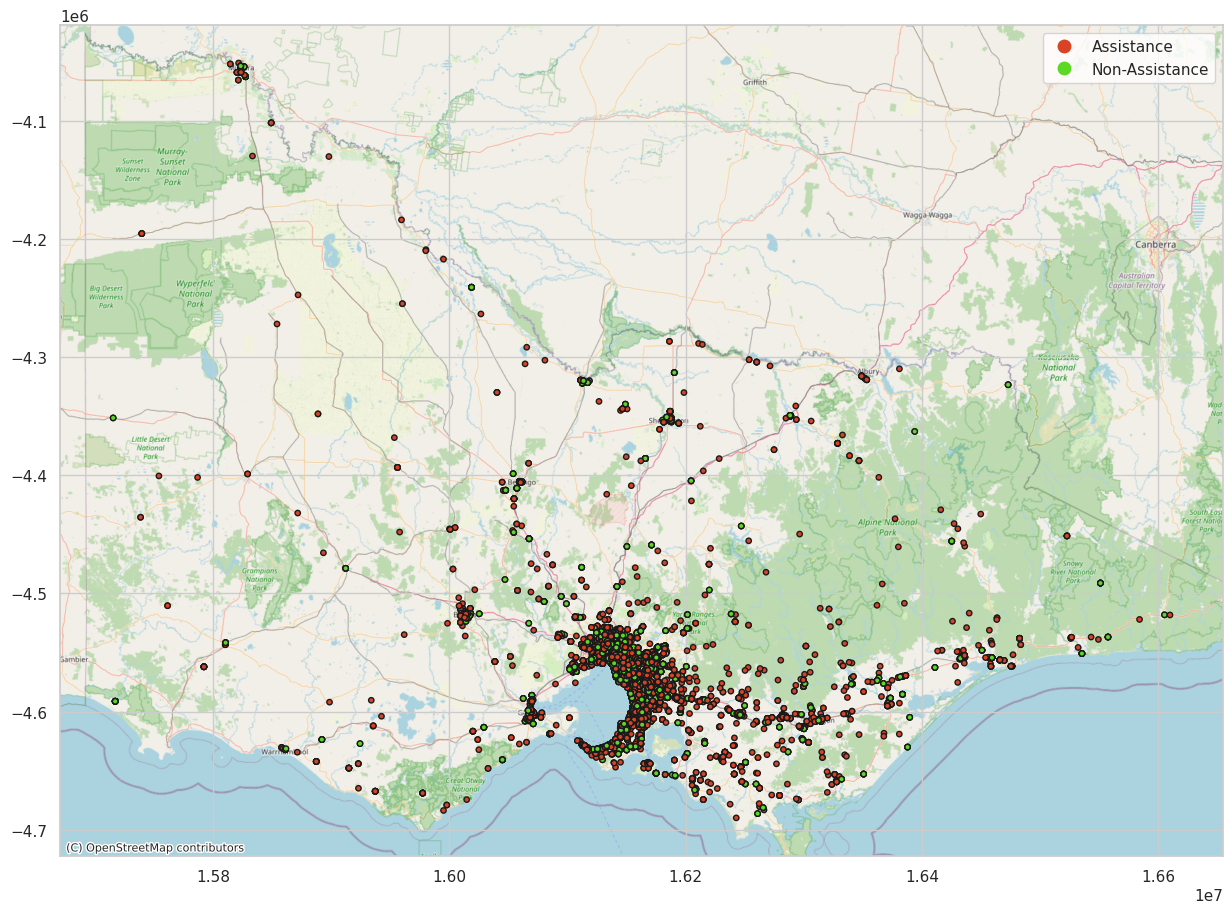
\includegraphics[width=120mm]{Figures/Victoria/original_OpenStreetMap.Mapnik.png}
		\label{VictoriaAccidentsMap:Original}
	}\\
	\subfloat[][Mapa de los accidentes filtrados de Victoria]{
		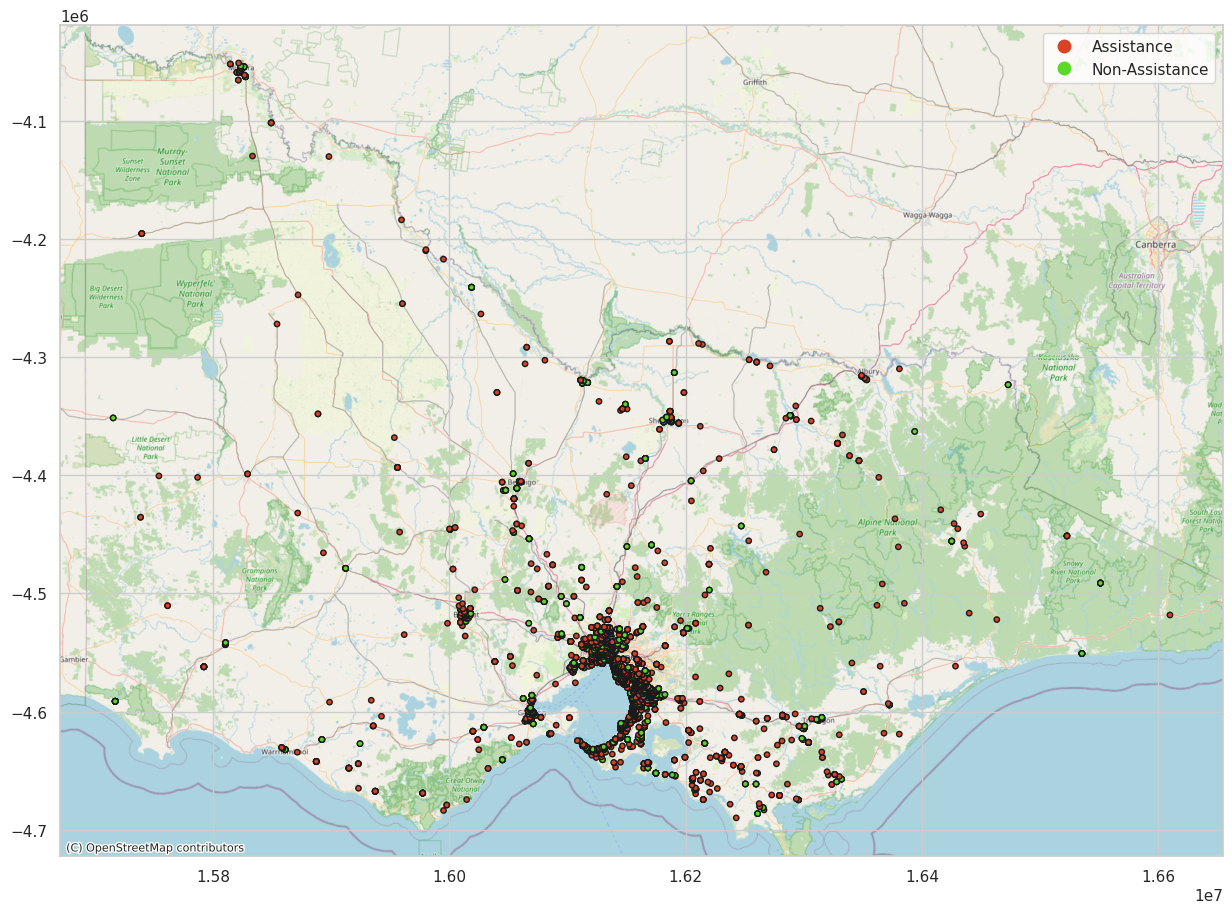
\includegraphics[width=120mm]{Figures/Victoria/filtered_OpenStreetMap.Mapnik.png}
		\label{VictoriaAccidentsMap:Filtered}
	}\\
	\caption{Mapa de accidentes de Victoria, original y filtrado.}
	\label{VictoriaAccidentsMap}
\end{figure}


En la Figura \ref{VictoriaLossFunction} se muestran las funciones \textit{F1-Score} sobre los datos de entrenamiento y validación para la región de Victoria. Esta métrica sobre el conjunto de entrenamiento muestra una curva de aprendizaje más lenta respecto a la anterior ciudad de Madrid, lo cual es comprensible ya que existe más variabilidad de datos en esta región al ser mucho más extensa que la anterior. La función de validación presenta más variaciones a lo largo del aprendizaje, llegando a su máximo aproximadamente en la época 45.

\begin{figure}[h!]
	\centering
	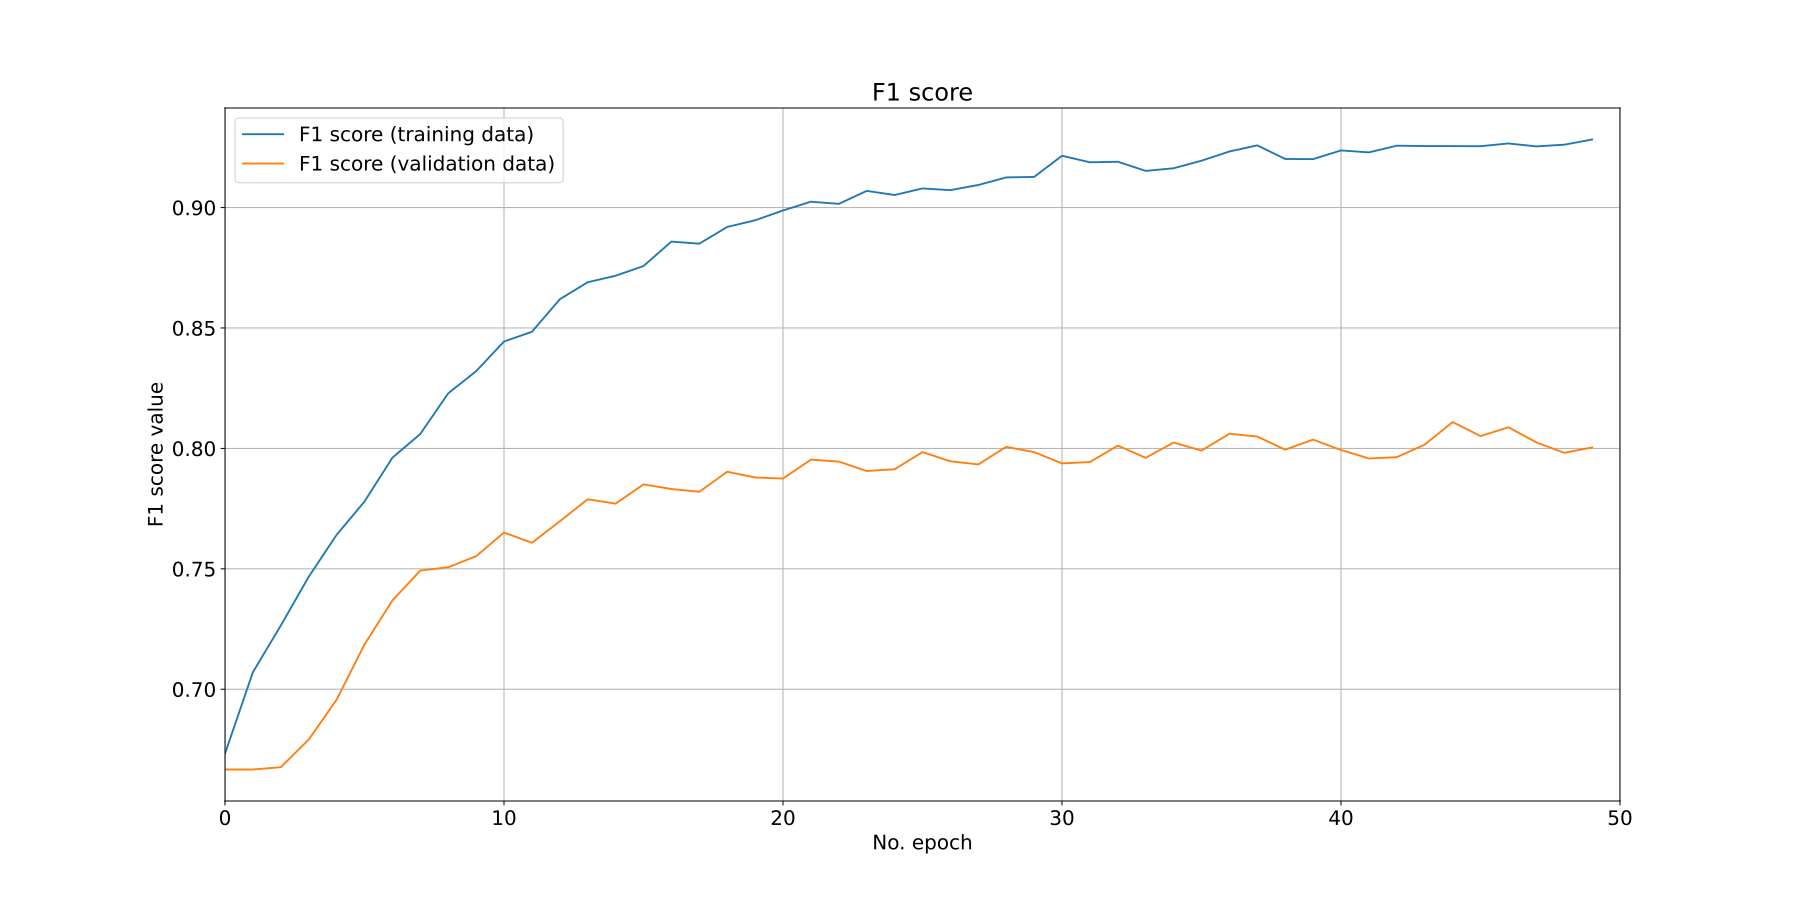
\includegraphics[width=14cm]{Figures/Victoria/Victoria_convolution_2d_f1_score_paper.png}
	\caption{Evolución de \textit{F1-Score} del modelo GTAAF en Victoria.}
	\label{VictoriaLossFunction}
\end{figure}

En la Tabla \ref{AustraliaMetrics}, se presentan los resultados del F1-Score obtenidos por cada uno de los modelos para ambos tipos de clasificación de accidentes. Concretamente, se observa que el nuevo modelo GTAAF logra una mejora del 6.5\% en comparación con el siguiente mejor modelo, el \textit{SVC}, para accidentes Sin Asistencia. Por otro lado, en lo que respecta a accidentes Con Asistencia, hay una mejora del 9\% en comparación con el \textit{MLP}. Estos resultados reflejan una mejora significativa en la capacidad de generalización del nuevo modelo propuesto.


%%%%%%%%%%%%%%%%%%%%%%%%%%%%%%%%%%%%%%%%%%%%%%%%%%%%%%%%%%%%%%%%%%%%%%%%%%%%%%%%%
\begin{table}[H]
	\caption{\textit{F1-Score} por modelo y clase de accidente en Victoria (Australia)}
	\begin{center}
		\begin{tabular}{|c|c||c|c|c|c|c|c|}
			\hline
			\multicolumn{2}{ |c|| }{} &
			\multicolumn{1}{ |c| }{\textbf{\textit{F1-Score} Australia}} \\ \hline
			
			\textbf{Modelo} & \textbf{Asistencia} & Victoria
			\\ \hline \hline
			
			\multirow{2}{*}{NB} &
			No &  0.635 \\ &
			Sí & 0.476 \\ \hline \hline
			\multirow{2}{*}{SVC} &
			No & 0.662 \\ &
			Sí &  0.679 \\ \hline \hline
			\multirow{2}{*}{KNN} &
			No  & 0.654 \\ &
			Sí & 0.616 \\ \hline \hline
			\multirow{2}{*}{RF} &
			No & 0.647 \\ &
			Sí & 0.364  \\ \hline \hline
			\multirow{2}{*}{LR} &
			No &  0.612 \\ &
			Sí & 0.630 \\ \hline \hline
			\multirow{2}{*}{MLP} &
			No & 0.635 \\ &
			Sí & 0.694 \\ \hline \hline
			\multirow{2}{*}{\textbf{GTAAF}} &
			\textbf{No} & \textbf{0.727} \\ &
			\textbf{Sí} & \textbf{0.784} \\ \hline \hline
		\end{tabular}
	\end{center}

	\label{AustraliaMetrics}
\end{table}
%%%%%%%%%%%%%%%%%%%%%%%%%%%%%%%%%%%%%%%%%%%%%%%%%%%%%%%%%%%%%%%%%%%%%%%%%%%%%%%%%

\subsubsection*{Reino Unido}

En este apartado se analizarán los datos proyectados sobre las distintas localidades escogidas de Reino Unido y sus respectivos resultados. Para ello en primer lugar se realizará un breve análisis de cada una de las regiones, posteriormente se interpretarán las evoluciones de los entrenamientos del modelo GTAAF para concluir con un análisis de resultados de los modelos aplicados sobre ellas.

\textbf{Southwark}\\

Southwark es un distrito de Londres situado en la orilla sur del río Támesis, con una alta densidad de población. En la Figura \ref{SouthwarkAccidentsMap} se observa la distribución de los accidentes a lo largo del municipio de Southwark. Analizando el conjunto de datos original, figura \ref{SouthwarkAccidentsMap:Original}, se observa que estos se producen a lo largo de las distintas vías que conectan el municipio con el centro neurálgico de la ciudad, hecho habitual al conectar zonas menos pobladas con lugares de trabajo y de ocio, mientras que la minoría de ellos se presentan en las calles circundantes. Observando la distribución de accidentes tras el proceso de filtrado por áreas (figura \ref{SouthwarkAccidentsMap:Filtered}) se acentúa este hecho, donde se observan que aquellos principales accidentes Con Asistencia se producen en estas vías. Por otra parte se muestra una concentración minoritaria de este tipo de accidentes en la zona de Dulwich (sur), en la intersección de la circunvalación \textit{S Circular} red con la carretera que dirige al centro del municipio.

%%%%%%%%%%%%%%%%%%%%%%%% DESCOMENTAR %%%%%%%%%%%%%%%%%%%%%%%%

\begin{figure}[H]
	\centering
	\subfloat[][Mapa de los accidentes originales de Southwark]{
		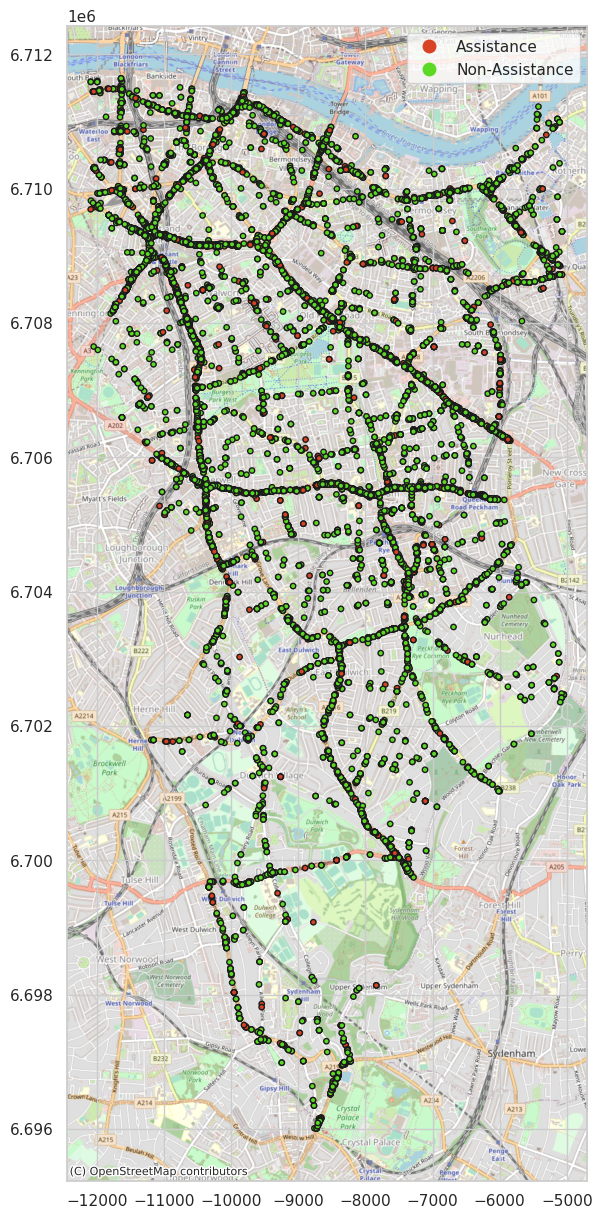
\includegraphics[width=70mm]{Figures/Southwark/original_OpenStreetMap.Mapnik.png}
		\label{SouthwarkAccidentsMap:Original}
	}
	\subfloat[][Mapa de los accidentes filtrados de Southwark]{
		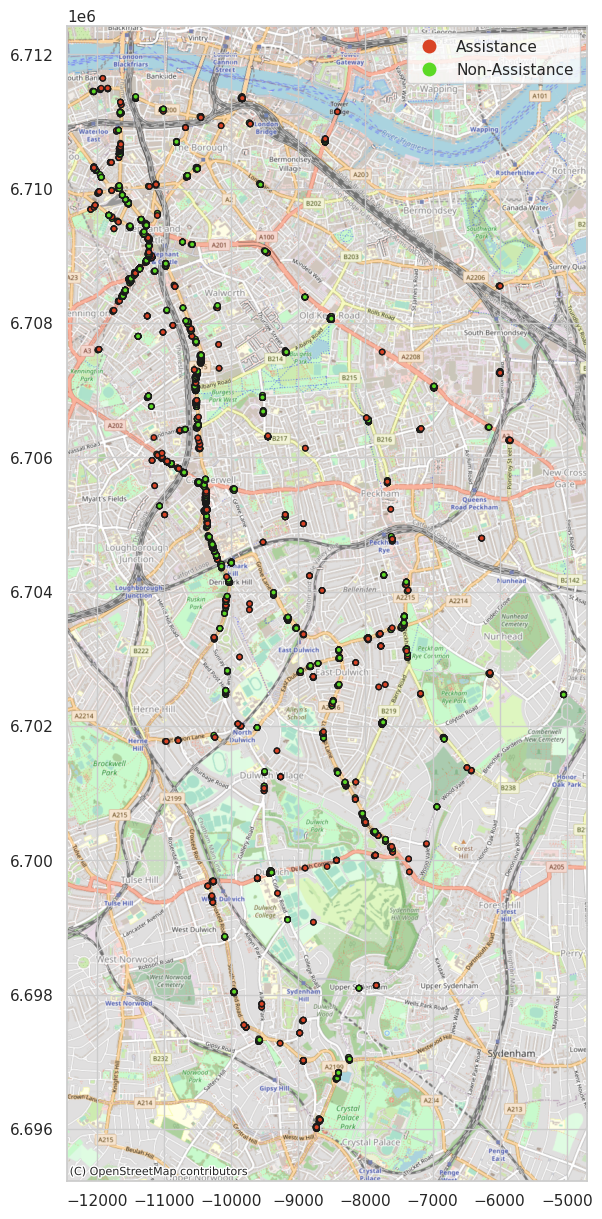
\includegraphics[width=70mm]{Figures/Southwark/filtered_OpenStreetMap.Mapnik.png}
		\label{SouthwarkAccidentsMap:Filtered}
	}
	\caption{Mapa de accidentes de Southwark, original y filtrado}
	\label{SouthwarkAccidentsMap}
\end{figure}


\textbf{Manchester}\\

Manchester, ubicada en el noroeste de Inglaterra, es una gran ciudad conocida por su legado industrial y su alta densidad de población. En la figura \ref{ManchesterAccidentsMap} se muestra la distribución de los accidentes de Manchester. Atendiendo a su distribución original, en la figura \ref{ManchesterAccidentsMap:Original}, como es habitual en cualquier población se aprecia una concentración de accidentes importante en la zona central de la ciudad, siendo también considerable en el área de Longsight. Por otra parte, las principales vías que comunican las periferias urbanas (norte) con el centro de la ciudad también presentan una concentración mayor de accidentes, lo que puede deberse a desplazamientos por motivos laborales o de ocio. Por otra parte, la carretera de Wythenshawe, cercano a Sale Water Park (Sur), también presenta una concentración elevada de accidentes, motivados por los desplazamientos de residencias personales. En la figura \ref{ManchesterAccidentsMap:Filtered} se observa la localización de los accidentes una vez se ha aplicado el proceso de filtrado por áreas, donde se vislumbra que gran parte de los accidentes Sin Asistencia se distribuyen a lo largo de las carreteras que comunican hacia el centro de la ciudad.

%%%%%%%%%%%%%%%%%%%%%%%% DESCOMENTAR %%%%%%%%%%%%%%%%%%%%%%%%

\begin{figure}[H]
	\centering
	\subfloat[][Mapa de los accidentes originales de Manchester]{
		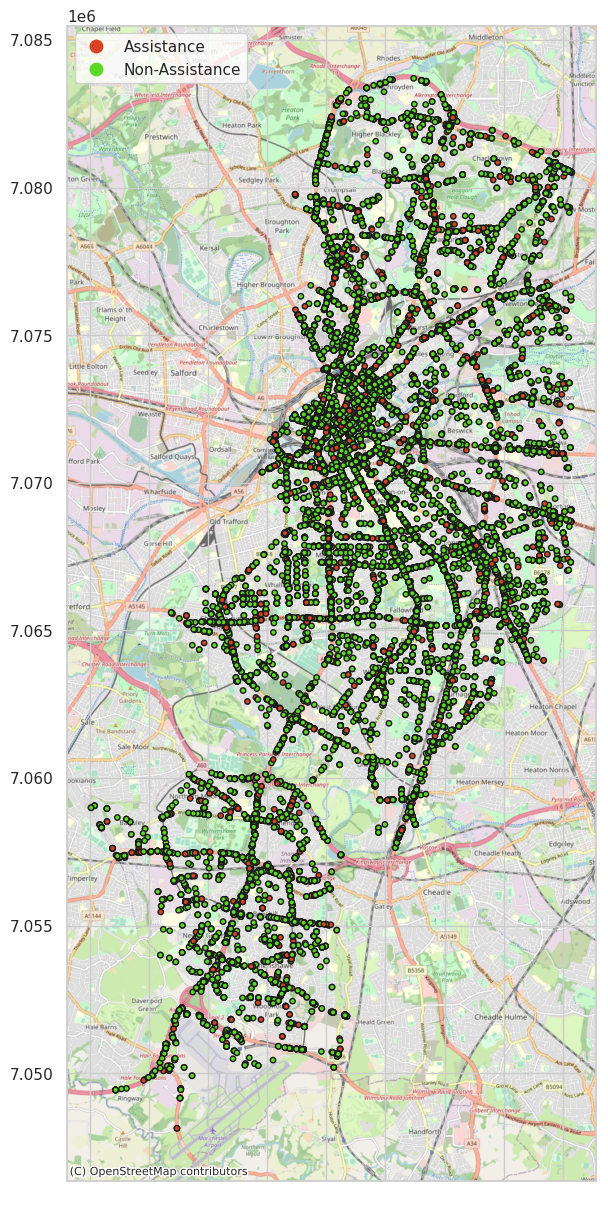
\includegraphics[width=70mm]{Figures/Manchester/original_OpenStreetMap.Mapnik.png}
		\label{ManchesterAccidentsMap:Original}
	}
	\subfloat[][Mapa de los accidentes filtrados de Manchester]{
		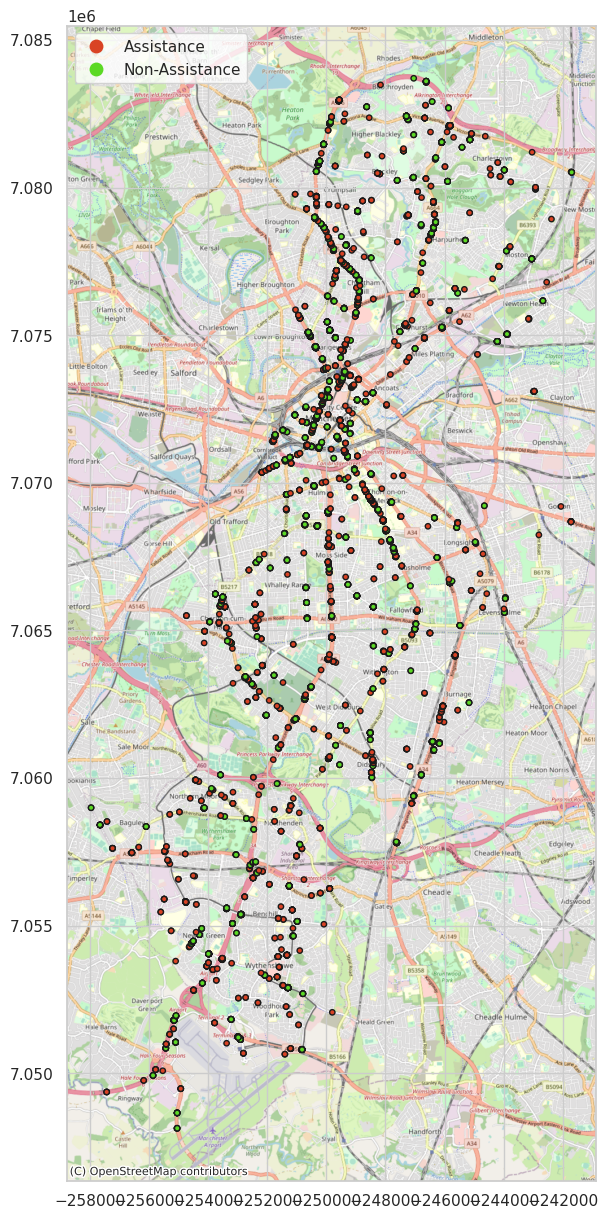
\includegraphics[width=70mm]{Figures/Manchester/filtered_OpenStreetMap.Mapnik.png}
		\label{ManchesterAccidentsMap:Filtered}
	}
	\caption{Mapa de accidentes de Manchester, original y filtrado}
	\label{ManchesterAccidentsMap}
\end{figure}

\textbf{Birmingham}\\

Birmingham es la segunda ciudad más grande de Inglaterra, se extiende por West Midlands con un panorama urbano diverso y una densidad de población considerable, famosa por su historia industrial y su vitalidad cultural. En la figura \ref{BirminghamAccidentsMap} se muestra la distribución de los accidentes de Birmingham, tanto los originales como los resultantes una vez aplicado el proceso de filtrado. Como se puede observar en los accidentes originales en la Figura \ref{BirminghamAccidentsMap:Original} se aprecia que gran parte de estos se concentran en la zona centro de la ciudad, una  tendencia normal debido a que es el principal foco de actividad de las ciudades. Mientras que los accidentes se van dispersando a medida que distan de este punto. Se aprecian ligeras agrupaciones de accidentes a lo largo de las zonas de incorporaciones a las principales arterias de la ciudad, como es al este, el caso de Handsworth. Por otra parte, en la figura \ref{BirminghamAccidentsMap:Filtered} se muestran los accidentes una vez se ha aplicado el proceso de filtrado por áreas. Como se puede observar, la información ha sido resumida sin dar lugar a pérdidas de valor en ella. Se visualizan ciertas zonas más conflictivas donde se producen accidentes más importantes, como es el caso de la carretera Holyhead Rd de entrada a la ciudad o en Northfield.

%%%%%%%%%%%%%%%%%%%%%%%% DESCOMENTAR %%%%%%%%%%%%%%%%%%%%%%%%

\begin{figure}[H]
	\centering
	\subfloat[][Mapa de los accidentes originales de Birmingham]{
		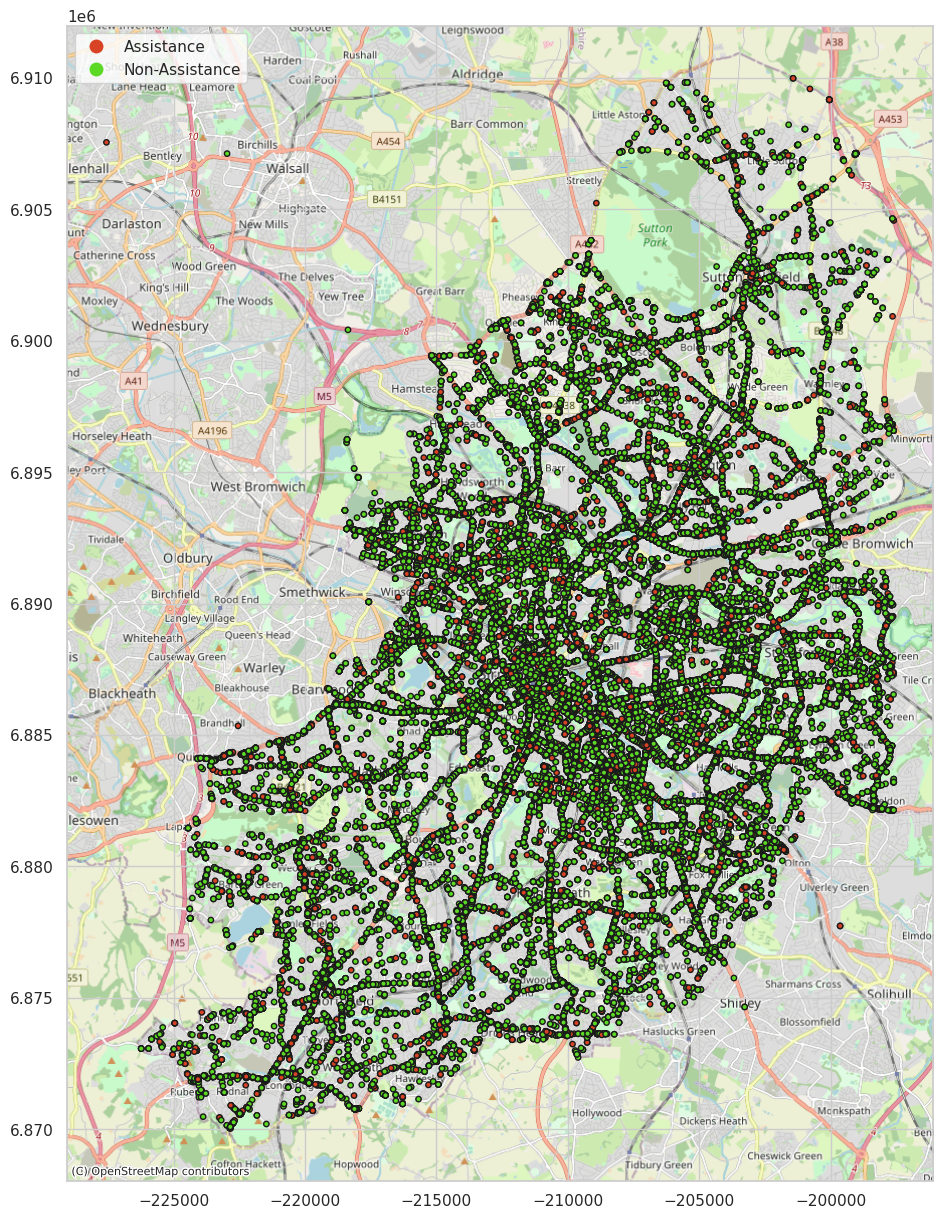
\includegraphics[width=70mm]{Figures/Birmingham/original_OpenStreetMap.Mapnik.png}
		\label{BirminghamAccidentsMap:Original}
	}
	\subfloat[][Mapa de los accidentes filtrados de Birmingham]{
		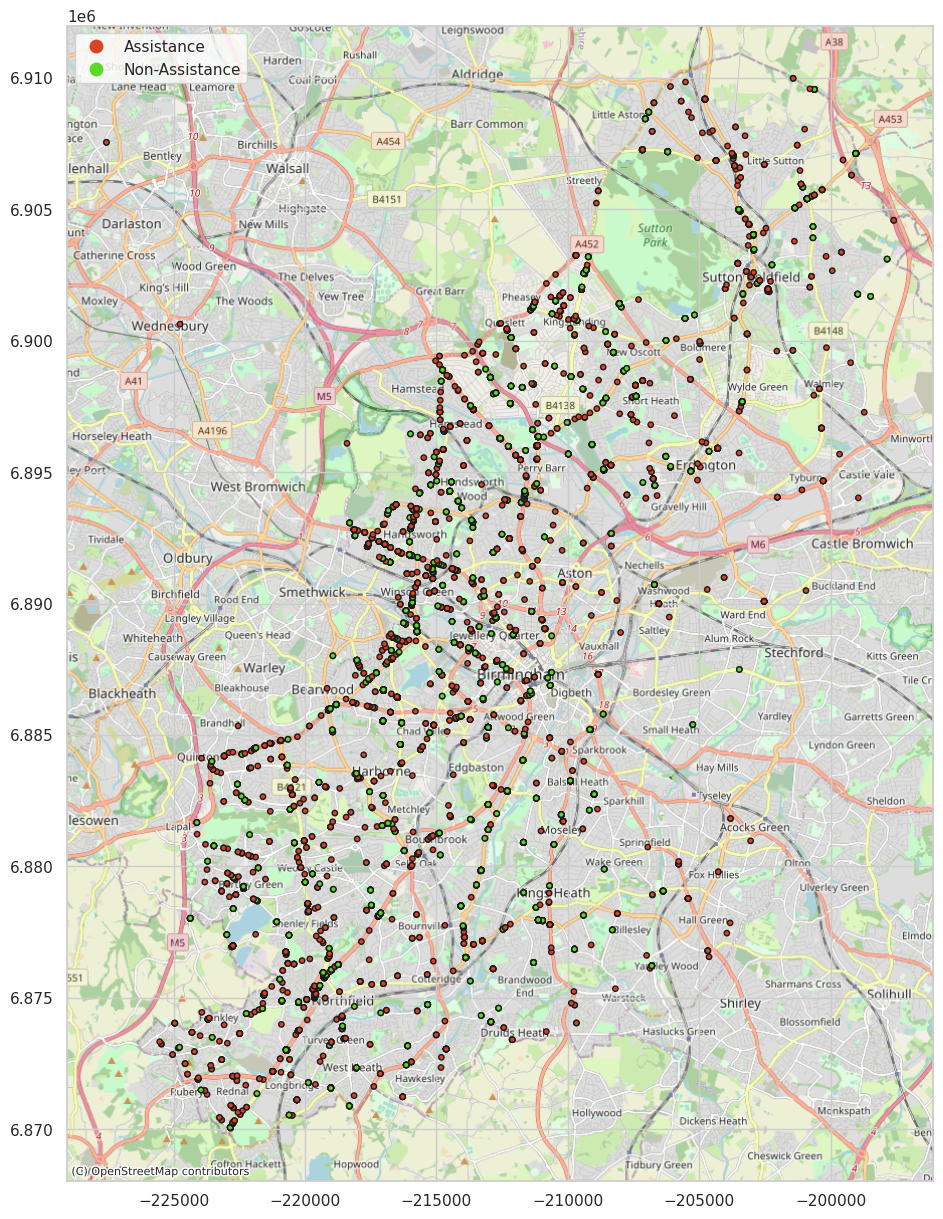
\includegraphics[width=70mm]{Figures/Birmingham/filtered_OpenStreetMap.Mapnik.png}
		\label{BirminghamAccidentsMap:Filtered}
	}
	\caption{Mapa de accidentes de Birmingham, original y filtrado}
	\label{BirminghamAccidentsMap}
\end{figure}


\textbf{Liverpool}\\

Liverpool, ubicada a lo largo del río Mersey en el noroeste de Inglaterra, prospera como una ciudad marítima con una rica historia, profundidad cultural y una densidad de población significativa, reconocida por su encanto en el frente marítimo y su legado musical. En la figura \ref{LiverpoolAccidentsMap} se muestra la comparativa de la distribución de accidentes originales del conjunto de datos y aquellos filtrados para esta ciudad. En la figura \ref{LiverpoolAccidentsMap:Original} se aprecian accidentes concentrados en la zona centro de la ciudad, como viene siendo habitual, además de a lo largo de las circunvalaciones que la rodean. En la figura \ref{LiverpoolAccidentsMap:Filtered}, después del proceso de filtrado, se aprecia que gran parte de los accidentes Con Asistencia se producen a lo largo de Strand Street (desde el sur hasta el oeste), convergiendo ambas direcciones en el centro neurálgico. Por otra parte se visualiza otra concentración en la carretera que conecta la localidad de Ormskirk con el centro (noroeste), una de las principales vías de conexión.

%%%%%%%%%%%%%%%%%%%%%%%% DESCOMENTAR %%%%%%%%%%%%%%%%%%%%%%%%


\begin{figure}[H]
	\centering
	\subfloat[][Mapa de los accidentes originales de Liverpool]{
		\includegraphics[width=70mm]{Figures/Liverpool/original_OpenStreetMap.Mapnik.png}
		\label{LiverpoolAccidentsMap:Original}
	}
	\subfloat[][Mapa de los accidentes filtrados de Liverpool]{
		\includegraphics[width=70mm]{Figures/Liverpool/filtered_OpenStreetMap.Mapnik.png}
		\label{LiverpoolAccidentsMap:Filtered}
	}
	\caption{Mapa de accidentes de Liverpool, original y filtrado}
	\label{LiverpoolAccidentsMap}
\end{figure}

\textbf{Sheffield}\\

Sheffield, ubicada en South Yorkshire, presume de un patrimonio industrial y paisajes pintorescos, con una densidad de población intermedia. En la figura \ref{SheffieldAccidentsMap} se muestra la distribución de accidentes para la ciudad, tanto la original como la resultante tras la etapa de filtrado. En la figura \ref{SheffieldAccidentsMap:Original} se pueden apreciar distintas concentraciones en zonas estratégicas. Como suele ser habitual, el núcleo urbano es un centro de mayor densidad de incidentes, mientras que en las intersecciones que conectan la ciudad de Sheffield y la de Rotherham (cruces de Tinsley Viaduct con Meadow Bank Road y la \textit{A6178}, al noreste de Sheffield). También se aprecian concentraciones en los suburbios de Wadsley Bridge y Malin Bridge, periferias de la ciudad, además de alrededor de todas las vías principales que conectan con el centro. Por otra parte, en la figura \ref{SheffieldAccidentsMap:Filtered} se muestran los accidentes una vez se ha realizado el proceso de filtrado, donde se aprecia que aquellos que han requerido de asistencia normalmente se presentan en las principales arterias, donde se circula a una mayor velocidad.

%%%%%%%%%%%%%%%%%%%%%%%% DESCOMENTAR %%%%%%%%%%%%%%%%%%%%%%%%

\begin{figure}[H]
	\centering
	\subfloat[][Mapa de los accidentes originales de Sheffield]{
		\includegraphics[width=75mm]{Figures/Sheffield/original_OpenStreetMap.Mapnik.png}
		\label{SheffieldAccidentsMap:Original}
	}
	\subfloat[][Mapa de los accidentes filtrados de Sheffield]{
		\includegraphics[width=75mm]{Figures/Sheffield/filtered_OpenStreetMap.Mapnik.png}
		\label{SheffieldAccidentsMap:Filtered}
	}
	\caption{Mapa de accidentes de Sheffield, original y filtrado}
	\label{SheffieldAccidentsMap}
\end{figure}


\textbf{Cornwall}\\

Cornwall, situada en la parte suroeste de Inglaterra con sus apacibles paisajes, encantadores pueblos costeros y extensiones rurales, fomenta un entorno tranquilo alejado de los núcleos de alta densidad de población. En la Figura \ref{CornwallAccidentsMap} se muestran de nuevo los accidentes originales de dataset y los que resultan tras aplicar el proceso de filtrado sobre el condado de Cornwall. En la Figura \ref{CornwallAccidentsMap:Original} las principales concentraciones de accidentes se encuentran distribuidas a lo largo de las distintas ciudades del condado. La mayoría de estos se encuentran divididos en dos regiones claramente definidas, la primera de ellas entre las vías que conectan las localidades de Camborne y Redruth (suroeste de Cornwall), y el área comprendida entre St Austell, Duporth, Carlyon Bay y Par, este del condado. No obstante, el resto de regiones también presentan una concentración considerable, como es el caso de la ciudad de Falmouth (sureste), las localidades de Penzance y Hayle (suroeste), en la ciudad de Newquay y sus alrededores (oeste), Bodmin (centro) y Launceston (norte). De nuevo, en este caso, se demuestra que la mayor frecuencia de accidentes se presenta entre los principales núcleos de población y las carreteras que los interconectan, debido a que las grandes ciudades implican más movimientos de vehículos. Atendiendo a la Figura \ref{CornwallAccidentsMap:Filtered} se observa que la ocurrencia de accidentes Con Asistencia, una vez aplicado el proceso de filtrado, tiene la misma tendencia que el expuesto para el conjunto de datos original, distribuyéndose a lo largo de las principales carreteras del condado Cornwall y concentrándose más en los núcleos de población.

%%%%%%%%%%%%%%%%%%%%%%%% DESCOMENTAR %%%%%%%%%%%%%%%%%%%%%%%%


\begin{figure}[H]
	\centering
	\subfloat[][Mapa de los accidentes originales de Cornwall]{
		\includegraphics[width=90mm]{Figures/Cornwall/original_OpenStreetMap.Mapnik.png}
		\label{CornwallAccidentsMap:Original}
	}\\
	\subfloat[][Mapa de los accidentes filtrados de Cornwall]{
		\includegraphics[width=90mm]{Figures/Cornwall/filtered_OpenStreetMap.Mapnik.png}
		\label{CornwallAccidentsMap:Filtered}
	}
	\caption{Mapa de accidentes de Cornwall, original y filtrado}
	\label{CornwallAccidentsMap}
\end{figure}

%%%%%%%%%%%%%%%%%%%%%%%% DESCOMENTAR %%%%%%%%%%%%%%%%%%%%%%%%

\textcolor{orange}{\textbf{LUIS: AQUÍ QUÉ COMENTAMOS?}}

\begin{figure}[H]
	\centering
	\subfloat[][Entrenamiento GTAAF en Southwark]{\includegraphics[width=80mm]{Figures/Cornwall/Cornwall_convolution_2d_f1_score_paper.png}}
	\subfloat[][Entrenamiento GTAAF en Manchester]{\includegraphics[width=80mm]{Figures/Manchester/Manchester_convolution_2d_f1_score_paper.png}}\\
	\subfloat[][Entrenamiento GTAAF en Birmingham]{\includegraphics[width=80mm]{Figures/Birmingham/Birmingham_convolution_2d_f1_score_paper.png}}
	\subfloat[][Entrenamiento GTAAF en Liverpool]{\includegraphics[width=80mm]{Figures/Liverpool/Liverpool_convolution_2d_f1_score_paper.png}}\\
	\subfloat[][Entrenamiento GTAAF en Sheffield]{\includegraphics[width=80mm]{Figures/Sheffield/Sheffield_convolution_2d_f1_score_paper.png}}
	\subfloat[][Entrenamiento GTAAF en Cornwall]{\includegraphics[width=80mm]{Figures/Cornwall/Cornwall_convolution_2d_f1_score_paper.png}}\\
	\caption{Evolución de \textit{F1-Score} del modelo GTAAF en las poblaciones de Reino Unido}
	\label{UKLossFunction}
\end{figure}


En la Tabla \ref{UKMetrics} se muestra el valor \textit{F1-Score} para cada una de las ciudades de cada modelo sobre el conjunto de test. Como se puede observar, el nuevo modelo propuesto GTAAF es el que mejor métricas ofrece en comparación al resto, obteniendo la mayor diferencia con respecto a su sucesor en los accidentes \textbf{Sin Asistencia}, el \textit{MLP}, para la ciudad de Manchester con un 6,7\%, mientras que la mayor diferencia para los accidentes \textbf{Con Asistencia} es de un 13.8\% en la ciudad de Southwark respecto al siguiente mejor modelo, de nuevo el \textit{MLP}. La siguiente mayor diferencia se presenta entre el modelo GTAAF se presenta en la ciudad de Southwark para la clase sin necesidad de asistencia, con un incremento del 4,8\% respecto al siguiente mejor modelo \textit{MLP}, mientras que para la clase con necesidad de asistencia ésta se presenta en la ciudad de Liverpool con respecto al modelo \textit{MLP}, llegando a un 13,2\%. Observando los resultados de la tabla, se aprecia que el mayor incremento del rendimiento con respecto al resto de modelos se presenta sobre la clase con necesidad de asistencia, obteniendo de media una mejora de 9,21\% sobre todas las ciudades, mientras que el incremento de rendimiento se acentúa menos en accidentes Sin Asistencia, ya que el resto de modelos ofrecen unas métricas más altas, siendo la mejora de un 3,93\% de media. Estos resultados reflejan una mejor generalización del modelo propuesto en comparación al resto de modelos estudiados para cada una de las ciudades de Reino Unido.

\begin{table}[H]
	\caption{\textit{F1-Score} por modelo y clase de accidente para cada una de las poblaciones de Reino Unido}
	\begin{center}
		\begin{tabular}{|c|c||c|c|c|c|c|c|}
			\hline
			\small
			\multicolumn{2}{ |c|| }{} &
			\multicolumn{6}{ |c| }{\textbf{\textit{F1-Score} Reino Unido}} \\ \hline
			
			\textbf{Modelo} & \textbf{Asistencia} & Southwark & Manchester & Birmingham & Liverpool & Sheffield & Cornwall
			\\ \hline \hline
			
			\multirow{2}{*}{NB} &
			No & 0.504 & 0.675 &  0.567 & 0.560 & 0.620 & 0.653 \\ &
			Sí & 0.400 & 0.482 & 0.558 & 0.417 & 0.669 & 0.484 \\ \hline \hline
			\multirow{2}{*}{SVC} &
			No & 0.826 & 0.845 & 0.812 & 0.865 & 0.809 & 0.702 \\ &
			Sí & 0.599 & 0.624 & 0.673 & 0.630 & 0.773 & 0.626 \\ \hline \hline
			\multirow{2}{*}{KNN} &
			No  & 0.652 & 0.723 & 0.747 & 0.746 & 0.754 & 0.656 \\ &
			Sí & 0.469 & 0.510 & 0.609 & 0.519 & 0.676 & 0.559 \\ \hline \hline
			\multirow{2}{*}{RF} &
			No & 0.561  & 0.118 & 0.303 & 0.742 & 0.313 & 0.711 \\ &
			Sí & 0.430 & 0.379 & 0.509 & 0.504 & 0.585 & 0.581 \\ \hline \hline
			\multirow{2}{*}{LR} &
			No & 0.711 & 0.800 & 0.761 & 0.806 & 0.733 & 0.630 \\ &
			Sí & 0.415 & 0.540 & 0.604 & 0.530 & 0.652 & 0.598 \\ \hline \hline
			\multirow{2}{*}{MLP} &
			No & 0.916 &  0.857 & 0.819 & 0.910 & 0.853 & 0.709 \\ &
			Sí & 0.743 & 0.632 & 0.662 & 0.721 & 0.810 & 0.671 \\ \hline \hline
			\multirow{2}{*}{\textbf     {GTAAF}} &
			\textbf{No} & \textbf{0.964} & \textbf{0.924} & \textbf{0.858} & \textbf{0.956} & \textbf{0.918} & \textbf{0.722} \\ &
			\textbf{Sí} & \textbf{0.881} & \textbf{0.762} & \textbf{0.711} & \textbf{0.853} & \textbf{0.889} & \textbf{0.707} \\ \hline \hline
		\end{tabular}
	\end{center}

	\label{UKMetrics}
\end{table}


La Figura \ref{GlobalSlightF1Score} muestra a modo de comparativa el rendimiento del nuevo modelo GTAAF propuesto en los accidentes \textbf{Sin Asistencia} para cada una de las poblaciones estudiadas respecto al resto de modelos del estado del arte con los que se ha experimentado en esta investigación. Se aprecia un incremento de rendimiento independientemente de las características individuales en todas las poblaciones respecto al resto de modelos estudiados, siendo el mayor incremento en la población de Victoria con un aumento del 6.5\% respecto al siguiente mejor modelo, el \textit{SVC}.

\begin{figure}[H]
	\centering
	\includegraphics[width=150mm]{Figures/Slight.png}
	\caption{Comparación de \textit{F1-Scores} para accidentes Sin Asistencia (GTAAF)}
	\label{GlobalSlightF1Score}
\end{figure}

La Figura \ref{GlobalAssistanceF1Score} muestra la comparativa del rendimiento basado en el F1-Score de los modelos para cada una de las ciudades en los accidentes \textbf{Con Asistencia}. En esta gráfica se puede observar una diferencia considerablemente mayor del nuevo modelo GTAAF. La mayor mejora se presenta en la ciudad de Southwark, con un incremento del \textit{F1-Score} del 13.8\% respecto al siguiente mejor modelo sobre esta población, el \textit{MLP}.

\begin{figure}[H]
	\centering
	\includegraphics[width=150mm]{Figures/Assistance.png}
	\caption{Comparación de \textit{F1-Scores} para accidentes Con Asistencia (GTAAF)}
	\label{GlobalAssistanceF1Score}
\end{figure}

\subsection{Pruebas de robustez}


En esta sección se realizarán distintas pruebas de estrés. El objetivo de estas pruebas es medir el rendimiento del modelo propuesto en casos extremos utilizando como base los conjuntos de datos expuestos en esta tesis para tener una aproximación del rendimiento del modelo en futuros conjuntos de datos que no dispongan de la totalidad de las características descritas en este documento. Para ello se realizarán tres experimentos para cada conjunto de datos, estos consistirán en eliminar aquellas variables de mayor y menor importancia de forma independiente, y, en un experimento posterior, se eliminarán ambas conjuntamente con el objetivo de medir el rendimiento ante la falta de características más y menos influyentes en futuros conjuntos de datos. La evaluación de la importancia de las características viene dada por el peso asignado a cada una de estas mediante el algoritmo \textit{XGBoost} optimizado mediante el algoritmo genético.

% \textcolor{orange}{\textbf{LUIS: Copiado y pegado del paper 3}}

Como se puede intuir en la Figura \ref{FeaturesClassification}, uno de los principales problemas en la generalización de un modelo es la disponibilidad de datos. Existen distintas características disponibles en cada conjunto de datos por distintos motivos. Uno de ellos puede ser la dificultad de extracción de información debido a razones económicas, sociales o políticas. Por ejemplo, tenemos el caso extremo de Madrid, que perdió toda una categoría (Driving Limitations)

Necesitamos probar la robustez y generalización del modelo descrito en esta investigación. Con este propósito, proponemos el tercer experimento: eliminar las variables que tienen la mayor y menor importancia para cada población basándonos en la importancia de cada característica durante el entrenamiento del algoritmo de impulso. Específicamente, se llevaron a cabo tres experimentos independientes para ambas poblaciones. El primero consistió en eliminar la variable con la menor importancia dentro de los datos, el segundo en eliminar la de mayor importancia, y el tercero en eliminar ambas simultáneamente.

Esta prueba de robustez se realizó en dos poblaciones: Cornwall (Reino Unido) y la población de Victoria, con el objetivo de simular nuevos conjuntos de datos donde no estén disponibles todos los datos mencionados en este documento.

En este análisis de resultados (consulte las Tablas \ref{CornwallLoss} y \ref{Victorialoss}), comparamos la brecha de rendimiento entre el nuevo modelo GTAAF propuesto y el mejor modelo posterior para cada experimento. Además, evaluaremos la diferencia en la métrica de F1-Score obtenida en comparación con los resultados presentados en secciones anteriores donde estas características estaban presentes.

%%%%%%%%%%%%%%%%%%%%%%%%%%%%%%%%%%%%%%%%%%%%%%%%%%%%%%%%%%%%%%%%%%%%%%%%%%%%%%%%%
\begin{table}[H]
	\caption[Comparativa \textit{F1-Score} con eliminación de características sobre Cornwall. Modelo GTAAF]{Comparativa \textit{F1-Score} con eliminación de características sobre Cornwall. Modelo GTAAF. La columna \textit{Menor} representa los resultados obtenidos ejecutando el modelo y eliminando la característica que menor peso presenta mediante el algoritmo genético, la columna \textit{Mayor} presenta los resultados eliminando la característica de mayor importancia y \textit{Ambas} presenta los resultados eliminando las dos simultáneamente. En negrita se muestran los resultados obtenidos por el mejor modelo (GTAAF)}
	\begin{center}
		\begin{tabular}{|c|c||c|c|c|c|c|c|}
			\hline
			\multicolumn{2}{ |c|| }{} &
			\multicolumn{3}{ |c| }{\textbf{Cornwall}} \\ \hline
			
			\textbf{Modelo} & Asistencia & Menor & Mayor & Ambas
			\\ \hline \hline
			
			\multirow{2}{*}{NB} &
			No & 0.668 & 0.597 & 0.592\\ &
			Sí  & 0.490 & 0.535 & 0.519 \\ \hline \hline
			\multirow{2}{*}{SVC} &
			No & 0.710 & 0.631 & 0.646\\ &
			Sí  & 0.628 & 0.626 & 0.620 \\ \hline \hline
			\multirow{2}{*}{KNN} &
			No & 0.671 & 0.601 & 0.637\\ &
			Sí  & 0.571 & 0.532 & 0.559 \\ \hline \hline
			\multirow{2}{*}{RF} &
			No & 0.719 & 0.498 & 0.514\\ &
			Sí  & 0.603 & 0.638 & 0.644 \\ \hline \hline
			\multirow{2}{*}{LR} &
			No & 0.670 & 0.575 & 0.567\\ &
			Sí  & 0.626 & 0.585 & 0.580 \\ \hline \hline
			\multirow{2}{*}{MLP} &
			No & 0.724 & 0.652 & 0.680\\ &
			Sí  & 0.695 & 0.654 & 0.685 \\ \hline \hline
			\multirow{2}{*}{\textbf{GTAAF}} &
			No & \textbf{0.768} & \textbf{0.736} & \textbf{0.792}\\ &
			Sí  & \textbf{0.766} & \textbf{0.736} & \textbf{0.787} \\ \hline \hline
		\end{tabular}
	\end{center}

	\label{CornwallLoss}
\end{table}
%%%%%%%%%%%%%%%%%%%%%%%%%%%%%%%%%%%%%%%%%%%%%%%%%%%%%%%%%%%%%%%%%%%%%%%%%%%%%%%%%


%%%%%%%%%%%%%%%%%%%%%%%%%%%%%%%%%%%%%%%%%%%%%%%%%%%%%%%%%%%%%%%%%%%%%%%%%%%%%%%%%
\begin{table}[H]
	\caption[Comparativa \textit{F1-Score} con eliminación de características sobre Victoria. Modelo GTAAF]{Comparativa \textit{F1-Score} con eliminación de características sobre Victoria. Modelo GTAAF. La columna \textit{Menor} representa los resultados obtenidos ejecutando el modelo y eliminando la característica que menor peso presenta mediante el algoritmo genético, la columna \textit{Mayor} presenta los resultados eliminando la característica de mayor importancia y \textit{Ambas} presenta los resultados eliminando las dos simultáneamente. En negrita se muestran los resultados obtenidos por el mejor modelo (GTAAF)}
	\begin{center}
		\begin{tabular}{|c|c||c|c|c|c|c|c|}
			\hline
			\multicolumn{2}{ |c|| }{} &
			\multicolumn{3}{ |c| }{\textbf{Victoria}} \\ \hline
			
			\textbf{Modelo} & Asistencia & Menor & Mayor & Ambas
			\\ \hline \hline
			
			\multirow{2}{*}{NB} &
			No & 0.639 & 0.613 & 0.607\\ &
			Sí  & 0.465 & 0.553 & 0.572 \\ \hline \hline
			\multirow{2}{*}{SVC} &
			No & 0.653 & 0.638 & 0.664\\ &
			Sí  & 0.657 & 0.650 & 0.676 \\ \hline \hline
			\multirow{2}{*}{KNN} &
			No & 0.625 & 0.627 & 0.638\\ &
			Sí  & 0.540 & 0.562 & 0.566 \\ \hline \hline
			\multirow{2}{*}{RF} &
			No & 0.630 & 0.630 & 0.621\\ &
			Sí  & 0.248 & 0.161 & 0.071 \\ \hline \hline
			\multirow{2}{*}{LR} &
			No & 0.598 & 0.574 & 0.599\\ &
			Sí  & 0.609 & 0.637 & 0.646 \\ \hline \hline
			\multirow{2}{*}{MLP} &
			No & 0.635 & 0.636 & 0.654\\ &
			Sí  & 0.693 & 0.686 & 0.692 \\ \hline \hline
			\multirow{2}{*}{\textbf{GTAAF}} &
			No & \textbf{0.732} & \textbf{0.720} & \textbf{0.778}\\ &
			Sí  & \textbf{0.780} & \textbf{0.793} & \textbf{0.814} \\ \hline \hline
		\end{tabular}
	\end{center}

	\label{Victorialoss}
\end{table}
%%%%%%%%%%%%%%%%%%%%%%%%%%%%%%%%%%%%%%%%%%%%%%%%%%%%%%%%%%%%%%%%%%%%%%%%%%%%%%%%%

En este experimento es necesario destacar un resultado: en nuestra propuesta, el modelo GTAAF, existe una gran mejora sobre los resultados del mismo modelo con todas las características. En contraste, hay un gran deterioro en los resultados de los otros modelos con los que se compara. En otras palabras, la diferencia en la puntuación \textit{F1-Score} entre GTAAF y los otros modelos aumenta. Esta circunstancia sugiere que nuestro modelo se ve afectado por las características extremas, donde el modelo de \textit{XGBoost} y el algoritmo genético favorecen y desfavorecen las características más y menos relevantes. Este no es el caso para los otros algoritmos, donde todas las características son individualizadas.

En la Figura \ref{lossFig} podemos observar la diferencia de los algoritmos con y sin pérdida de características (Tablas \ref{UKMetrics}, columna Cornwall, y \ref{AustraliaMetrics} contra las Tablas \ref{CornwallLoss} y \ref{Victorialoss} respectivamente). Mostramos cómo nuestro modelo mejora sus propios resultados en todos los casos. Por ejemplo, en Cornwall, obtenemos una mejora en nuestro modelo del 4.8\% y 5.9\% en los accidentes \textbf{Sin Asistencia} y \textbf{Con Asistencia} (eliminando la peor característica, ver la barra azul en la Figura \ref{lossFig}-arriba), 1.4\% y 2.9\% (eliminando la mejor característica, ver la barra verde en la Figura \ref{lossFig}-arriba) y 7\% y 8\% (eliminando ambas características, ver la barra gris en la Figura \ref{lossFig}-arriba), respectivamente. Evaluando un área más dispersa como Victoria, los resultados son similares pero con una mejora menor: 0.5\% y 0.4\% (ver la barra azul en la Figura \ref{lossFig}-abajo), -0.7\% y 0.9\% (ver la barra verde en la Figura \ref{lossFig}-abajo), y 5.1\% y 3\% (ver la barra gris en la Figura \ref{lossFig}-abajo), respectivamente. Esto indicaría un efecto menor de los valores extremos en la ponderación del algoritmo genético si el área es más dispersa.

\begin{figure}[H]
	\centering
	\includegraphics[width=150mm]{Figures/LossFeatures/loss.png}
	\caption[Comparación de pérdida de características del modelo GTAAF]{Comparación de pérdida de características del modelo GTAAF. Las barras representan la diferencia entre los resultados con todas las características y los resultados sin características extremas: en azul sin la característica más baja, en verde sin la característica más alta y en gris sin ambas características extremas}
	\label{lossFig}
\end{figure}

 

\chapter{Conclusiones}


En esta tesis se ha propuesto un nuevo modelo que evalúa la necesidad de asistencia médica en los accidentes de tráfico. Esta funcionalidad es extremadamente importante para priorizar la asignación de recursos médicos una vez se conocen las características del accidente, de tal forma que se puedan minimizar las consecuencias físicas a corto y largo plazo de los afectados. Para ello se ha propuesto un modelo que transforma las características que describen los accidentes, mediante categorizaciones, en datos matriciales para alimentar a nuestro modelo convolucional GTAAF. Como se ha demostrado en su evaluación, los resultados no solo mejoran ampliamente a los modelos del estado del arte (con valores de hasta el 13.8\%), sino que la categorización propuesta ha demostrado robustez respecto a la interpretación de las características de forma individual de los demás modelos. Además, nuestro modelo ha mostrado un gran rendimiento en distintos contextos, concretamente en  distintos datasets de 8 poblaciones de diferentes densidades de población.\\

Además, con el objetivo de proponer un modelo general que pueda ser aplicado a nuevas poblaciones que no dispongan de la misma información que los datasets presentados en este artículo (debido principalmente a la dificultad inherente de recogida de datos específicos, como controles de alcohol y drogas, u otras características cuya obtención esté relacionada con la condición económica de la población), se ha analizado la robustez del modelo eliminando características, excluyendo aquellas de mayor y menor impacto que han resultado del \textit{XGBoost} optimizado mediante el algoritmo genético, obteniendo resultados incluso mejores en nuestro modelo. Esto hace indicar la sensibilidad que tiene respecto a estos casos extremos.

Como principal medida medida como trabajo a futuro se propone aplicar este modelo a otros conjuntos de datos de accidentes para evaluar la utilidad que ofrece en comparación con otros modelos, por otra parte se debe analizar cómo reducir la sensibilidad del modelo GTAAF ante características extremas.


 

\chapter{Publicaciones}

1. \textbf{Pérez-Sala, L.}, Curado, M., Tortosa, L., \& Vicent, J. F. (2023). Deep learning model of convolutional neural networks powered by a genetic algorithm for prevention of traffic accidents severity. Chaos, Solitons \& Fractals, 169, 113245.\\

\textbf{Indicadores de calidad:} 
\begin{itemize}
	\item Factor de impacto: 9.992
	\item Ranking: 1/108 (MATHEMATICS, INTERDISCIPLINARY APPLICATIONS)
	\item Cuartil: Q1
\end{itemize}

\textbf{Resumen.} La Organización Mundial de la Salud destaca que el número de muertes anuales por accidentes de tráfico ha alcanzado los 1,35 millones (Informe Mundial sobre la Situación de la Seguridad Vial 2018). Además, millones de personas sufren lesiones más o menos graves como consecuencia de este tipo de accidentes. En este escenario, la predicción de la gravedad de los accidentes de tráfico es un punto esencial cuando se trata de mejorar la prevención y la reacción de las entidades responsables. Por otro lado, el desarrollo de metodologías confiables para predecir y clasificar el nivel de gravedad de los accidentes de tráfico, basado en diversas variables, es un componente clave en el campo de investigación en seguridad vial. Este trabajo tiene como objetivo proponer un nuevo enfoque, basado en redes neuronales convolucionales, para la detección de la gravedad de los accidentes de tráfico. Detrás de este objetivo se encuentra la limpieza, análisis y visualización de datos, así como el diseño, implementación y comparación de modelos de aprendizaje automático considerando la precisión como indicador de rendimiento.
Con este propósito, se ha implementado una metodología escalable y fácilmente reutilizable. Esta metodología se ha comparado con otros modelos de aprendizaje profundo, verificando que los resultados de la red neuronal diseñada ofrecen un mejor rendimiento en términos de medidas de calidad.\\


2. \textbf{Pérez-Sala, L.}, Curado, M., Tortosa, L., \& Vicent, J. F. Increasing the accuracy of a deep learning model for traffic accident severity prediction by adding a temporal category. En International Conference on Advances in Computing Research, Madrid (3-5 Junio 2024). Estado: Aceptado.\\

\textbf{Indicadores de calidad:} 
\begin{itemize}
	\item Tipo de congreso: Internacional
	\item Ranking: CORE C
\end{itemize}

\textbf{Resumen.} La inteligencia artificial se ha convertido en una herramienta ampliamente utilizada en el contexto de la movilidad urbana y las aplicaciones de seguridad vial. Este artículo se centra en predecir la gravedad de los accidentes utilizando características que se pueden recopilar de manera fácil y rápida. Proponemos un modelo de aprendizaje profundo basado en una red neuronal convolucional que se compara, desde el punto de vista del rendimiento, con varios modelos de aprendizaje profundo para predecir la gravedad de las colisiones de tráfico. Nuestra propuesta modifica un modelo anterior al refinar la categorización del accidente, implementar un filtro de área para abordar los datos desequilibrados, reorganizar el conjunto de datos en diferentes características basadas en su naturaleza y discretizar el tiempo de los accidentes mediante funciones seno y coseno. Este trabajo demuestra un rendimiento superior a seis modelos de aprendizaje profundo, logrando una mejora importante en la predicción de las dos categorías analizadas (accidentes que requieren asistencia y los que no la requieren). \\


3. \textbf{Pérez-Sala, L.}, Curado, M., Oliver, J. L., \& Vicent, J. F. (2023). A General Approach to Predict the Traffic Accident Assistance Based on Deep Learning. Applied Soft Computing. Estado: Under Review .\\

\textbf{Indicadores de calidad:} 
\begin{itemize}
	\item Factor de impacto: 8.7
	\item Ranking: 12/110 (COMPUTER SCIENCE, INTERDISCIPLINARY APPLICATIONS)
	
	\item Cuartil: Q1
\end{itemize}

\textbf{Resumen.} Ante el problema de los numerosos accidentes de tráfico que ocurren diariamente, es crucial  la predicción de la necesidad de asistencia médica en estos accidentes, lo cual ha sido estudiado en numerosos trabajos que abordan cuestiones como los datos desequilibrados. Con este propósito, proponemos un modelo de aprendizaje profundo para analizar la asistencia en los accidentes, cuyo objetivo final es distinguir si un accidente requiere asistencia médica o no. Nuestra perspectiva es general, de modo que el modelo sea válido para cualquier ciudad. Para lograrlo, presentamos un modelo dividido en tres etapas claramente diferenciadas. En la etapa de pre-procesamiento, se realiza un tratamiento de datos. En segundo lugar, en la etapa de postprocesamiento, se emplean algoritmos genéticos y de impulso para obtener la importancia de todas las variables del conjunto de datos utilizadas en la predicción. Finalmente, evaluamos la eficacia y precisión del modelo aplicándolo a accidentes de tráfico en seis ciudades diferentes. Los resultados experimentales muestran que el modelo propuesto logra una mayor precisión en todas las ciudades en comparación con seis modelos de vanguardia. Los resultados confirman la idoneidad y aplicabilidad del propuesto modelo generalizado de aprendizaje profundo para detectar la asistencia en accidentes de tráfico. \\


4. \textbf{Pérez-Sala, L.}, Curado, M. \& Vicent, J. F. (2023). Features Fusion for a Robust Traffic Accidents Assistance Forecasting Model with Deep Learning. Expert Systems with Applications. Estado: Under Review.\\

\textbf{Indicadores de calidad:} 
\begin{itemize}
	\item Factor de impacto: 8.5
	\item Ranking: 24/145 (COMPUTER SCIENCE, ARTIFICIAL INTELLIGENCE)
	\item Cuartil: Q1
\end{itemize}

\textbf{Resumen.} Los accidentes de tráfico representan un problema muy importante tanto desde un punto de vista social como económico, y pueden considerarse como un obstáculo que frena el desarrollo de los países. En los accidentes de carretera, muchas personas pierden la vida debido a la falta de asistencia médica. La provisión oportuna de atención de emergencia puede reducir la tasa de mortalidad, así como la gravedad de los accidentes. En este estudio, predecimos la gravedad de los accidentes de tráfico en términos de la necesidad de asistencia utilizando aprendizaje profundo para que las autoridades competentes lo utilicen en la gestión de la atención médica. En este trabajo, proponemos un modelo general para la predicción de asistencia en accidentes de tráfico llamado GTAAF, que utiliza una red neuronal convolucional alimentada por matrices construidas mediante algoritmos evolutivos y modelos de tipo boosting. Se realizaron experimentos con datos de accidentes de tráfico de ocho áreas del Reino Unido, España y Australia en los últimos años. Para evaluar la eficiencia del modelo presentado, se comparó con seis modelos de aprendizaje automático de vanguardia, mostrando una mejora en precisión, recall y F1-score. Además, se probó la robustez de la propuesta eliminando variables extremas de los conjuntos de datos, obteniendo mejoras significativas respecto a los demás modelos.


\chapter{Publicaciones}

1. \textbf{Pérez-Sala, L.}, Curado, M., Tortosa, L., \& Vicent, J. F. (2023). Deep learning model of convolutional neural networks powered by a genetic algorithm for prevention of traffic accidents severity. Chaos, Solitons \& Fractals, 169, 113245.\\

\textbf{Indicadores de calidad:} 
\begin{itemize}
	\item Factor de impacto: 9.992
	\item Ranking: 1/108 (MATHEMATICS, INTERDISCIPLINARY APPLICATIONS)
	\item Cuartil: Q1
\end{itemize}

\textbf{Resumen.} La Organización Mundial de la Salud destaca que el número de muertes anuales por accidentes de tráfico ha alcanzado los 1,35 millones (Informe Mundial sobre la Situación de la Seguridad Vial 2018). Además, millones de personas sufren lesiones más o menos graves como consecuencia de este tipo de accidentes. En este escenario, la predicción de la gravedad de los accidentes de tráfico es un punto esencial cuando se trata de mejorar la prevención y la reacción de las entidades responsables. Por otro lado, el desarrollo de metodologías confiables para predecir y clasificar el nivel de gravedad de los accidentes de tráfico, basado en diversas variables, es un componente clave en el campo de investigación en seguridad vial. Este trabajo tiene como objetivo proponer un nuevo enfoque, basado en redes neuronales convolucionales, para la detección de la gravedad de los accidentes de tráfico. Detrás de este objetivo se encuentra la limpieza, análisis y visualización de datos, así como el diseño, implementación y comparación de modelos de aprendizaje automático considerando la precisión como indicador de rendimiento.
Con este propósito, se ha implementado una metodología escalable y fácilmente reutilizable. Esta metodología se ha comparado con otros modelos de aprendizaje profundo, verificando que los resultados de la red neuronal diseñada ofrecen un mejor rendimiento en términos de medidas de calidad.\\


2. \textbf{Pérez-Sala, L.}, Curado, M., Tortosa, L., \& Vicent, J. F. Increasing the accuracy of a deep learning model for traffic accident severity prediction by adding a temporal category. En International Conference on Advances in Computing Research, Madrid (3-5 Junio 2024). Estado: Aceptado.\\

\textbf{Indicadores de calidad:} 
\begin{itemize}
	\item Tipo de congreso: Internacional
	\item Ranking: CORE C
\end{itemize}

\textbf{Resumen.} La inteligencia artificial se ha convertido en una herramienta ampliamente utilizada en el contexto de la movilidad urbana y las aplicaciones de seguridad vial. Este artículo se centra en predecir la gravedad de los accidentes utilizando características que se pueden recopilar de manera fácil y rápida. Proponemos un modelo de aprendizaje profundo basado en una red neuronal convolucional que se compara, desde el punto de vista del rendimiento, con varios modelos de aprendizaje profundo para predecir la gravedad de las colisiones de tráfico. Nuestra propuesta modifica un modelo anterior al refinar la categorización del accidente, implementar un filtro de área para abordar los datos desequilibrados, reorganizar el conjunto de datos en diferentes características basadas en su naturaleza y discretizar el tiempo de los accidentes mediante funciones seno y coseno. Este trabajo demuestra un rendimiento superior a seis modelos de aprendizaje profundo, logrando una mejora importante en la predicción de las dos categorías analizadas (accidentes que requieren asistencia y los que no la requieren). \\


3. \textbf{Pérez-Sala, L.}, Curado, M., Oliver, J. L., \& Vicent, J. F. (2023). A General Approach to Predict the Traffic Accident Assistance Based on Deep Learning. Applied Soft Computing. Estado: Under Review .\\

\textbf{Indicadores de calidad:} 
\begin{itemize}
	\item Factor de impacto: 8.7
	\item Ranking: 12/110 (COMPUTER SCIENCE, INTERDISCIPLINARY APPLICATIONS)
	
	\item Cuartil: Q1
\end{itemize}

\textbf{Resumen.} Ante el problema de los numerosos accidentes de tráfico que ocurren diariamente, es crucial  la predicción de la necesidad de asistencia médica en estos accidentes, lo cual ha sido estudiado en numerosos trabajos que abordan cuestiones como los datos desequilibrados. Con este propósito, proponemos un modelo de aprendizaje profundo para analizar la asistencia en los accidentes, cuyo objetivo final es distinguir si un accidente requiere asistencia médica o no. Nuestra perspectiva es general, de modo que el modelo sea válido para cualquier ciudad. Para lograrlo, presentamos un modelo dividido en tres etapas claramente diferenciadas. En la etapa de pre-procesamiento, se realiza un tratamiento de datos. En segundo lugar, en la etapa de postprocesamiento, se emplean algoritmos genéticos y de impulso para obtener la importancia de todas las variables del conjunto de datos utilizadas en la predicción. Finalmente, evaluamos la eficacia y precisión del modelo aplicándolo a accidentes de tráfico en seis ciudades diferentes. Los resultados experimentales muestran que el modelo propuesto logra una mayor precisión en todas las ciudades en comparación con seis modelos de vanguardia. Los resultados confirman la idoneidad y aplicabilidad del propuesto modelo generalizado de aprendizaje profundo para detectar la asistencia en accidentes de tráfico. \\


4. \textbf{Pérez-Sala, L.}, Curado, M. \& Vicent, J. F. (2023). Features Fusion for a Robust Traffic Accidents Assistance Forecasting Model with Deep Learning. Expert Systems with Applications. Estado: Under Review.\\

\textbf{Indicadores de calidad:} 
\begin{itemize}
	\item Factor de impacto: 8.5
	\item Ranking: 24/145 (COMPUTER SCIENCE, ARTIFICIAL INTELLIGENCE)
	\item Cuartil: Q1
\end{itemize}

\textbf{Resumen.} Los accidentes de tráfico representan un problema muy importante tanto desde un punto de vista social como económico, y pueden considerarse como un obstáculo que frena el desarrollo de los países. En los accidentes de carretera, muchas personas pierden la vida debido a la falta de asistencia médica. La provisión oportuna de atención de emergencia puede reducir la tasa de mortalidad, así como la gravedad de los accidentes. En este estudio, predecimos la gravedad de los accidentes de tráfico en términos de la necesidad de asistencia utilizando aprendizaje profundo para que las autoridades competentes lo utilicen en la gestión de la atención médica. En este trabajo, proponemos un modelo general para la predicción de asistencia en accidentes de tráfico llamado GTAAF, que utiliza una red neuronal convolucional alimentada por matrices construidas mediante algoritmos evolutivos y modelos de tipo boosting. Se realizaron experimentos con datos de accidentes de tráfico de ocho áreas del Reino Unido, España y Australia en los últimos años. Para evaluar la eficiencia del modelo presentado, se comparó con seis modelos de aprendizaje automático de vanguardia, mostrando una mejora en precisión, recall y F1-score. Además, se probó la robustez de la propuesta eliminando variables extremas de los conjuntos de datos, obteniendo mejoras significativas respecto a los demás modelos.

%%%%%%%%%%%%%%%%%%%%%%%%%%%%%%%%%%%%%%%%%%%%%%%%%%%%%%%%%%%%%%%%%%%%%%%%%%%%%%%%%%%%%%%%%%%%%%%%%%%%%%%%%%%%%%%%%%%%%%%%

%%%%%%%%%%%%%%%%%%%%%%%%%%%%%%%%%%%%%%%%%%%%%%%%%%%%%%%%%%%%%%%%%%%%%%%%%%%%%%%%%%%%%%%%%%%%%%%%%%%%%%%%%%%%%%%%%%%%%%%%
% PAGINAS: APÉNDICES
%:Empezamos con los apéndices, que irían en uno o más ficheros. Es necesario incluir estos ficheros entre el entorno \begin{appendices}....\end{appendices} debido a que se ha deseado utilizar un formato diferente para el título de los apéndices, incluyendo la palabra apéndice, para la numeración de los apéndices, alfabético, y para las cabeceras de las páginas.

%\begin{appendices}
% Fichero en el que se incluyen los apéndices
%%APENDICE A
\chapter{Conjuntos de datos y redes urbanas}\label{CAP_07}
 %Ver este fichero para incluir ahí los apéndices.
%\end{appendices}
%:Fin de la inclusión de apéndices
%%%%%%%%%%%%%%%%%%%%%%%%%%%%%%%%%%%%%%%%%%%%%%%%%%%%%%%%%%%%%%%%%%%%%%%%%%%%%%%%%%%%%%%%%%%%%%%%%%%%%%%%%%%%%%%%%%%%%%%%

%:Empieza todo lo que no constituye el cuerpo en si del libro. Todo lo que va detrás
\backmatter

%%%%%%%%%%%%%%%%%%%%%%%%%%%%%%%%%%%%%%%%%%%%%%%%%%%%%%%%%%%%%%%%%%%%%%%%%%%%%%%%%%%%%%%%%%%%%%%%%%%%%%%%%%%%%%%%%%%%%%%%
% PAGINAS: ÍNDICE DE FIGURAS
%:Indice de figuras, coméntese las siguientes líneas si no se desea
%\cleardoublepage
%\phantomsection
%:Para añadir una línea en blanco en el TOC y separar esta lista
%\addtocontents{toc}{\protect\mbox{}\protect\hspace*{0pt}\par}
%\addcontentsline{toc}{listasb}{\listfigurename}
%\pagestyle{especial}
%\listoffigures
%%%%%%%%%%%%%%%%%%%%%%%%%%%%%%%%%%%%%%%%%%%%%%%%%%%%%%%%%%%%%%%%%%%%%%%%%%%%%%%%%%%%%%%%%%%%%%%%%%%%%%%%%%%%%%%%%%%%%%%%

%%%%%%%%%%%%%%%%%%%%%%%%%%%%%%%%%%%%%%%%%%%%%%%%%%%%%%%%%%%%%%%%%%%%%%%%%%%%%%%%%%%%%%%%%%%%%%%%%%%%%%%%%%%%%%%%%%%%%%%%
% PAGINAS: ÍNDICE DE TABLAS
%:Indice de tablas, coméntese las siguientes líneas si no se desea
%\cleardoublepage
%\phantomsection
%\addcontentsline{toc}{listasb}{\listtablename}
%\pagestyle{especial}
%\listoftables
%%%%%%%%%%%%%%%%%%%%%%%%%%%%%%%%%%%%%%%%%%%%%%%%%%%%%%%%%%%%%%%%%%%%%%%%%%%%%%%%%%%%%%%%%%%%%%%%%%%%%%%%%%%%%%%%%%%%%%%%

%%%%%%%%%%%%%%%%%%%%%%%%%%%%%%%%%%%%%%%%%%%%%%%%%%%%%%%%%%%%%%%%%%%%%%%%%%%%%%%%%%%%%%%%%%%%%%%%%%%%%%%%%%%%%%%%%%%%%%%%
% PAGINAS: ÍNDICE DE PROGRAMAS
%:Indice de Programas
%\cleardoublepage
%\phantomsection
%\addcontentsline{toc}{listasb}{\lstlistlistingname}
%\pagestyle{especial}
%\lstlistoflistings
%%%%%%%%%%%%%%%%%%%%%%%%%%%%%%%%%%%%%%%%%%%%%%%%%%%%%%%%%%%%%%%%%%%%%%%%%%%%%%%%%%%%%%%%%%%%%%%%%%%%%%%%%%%%%%%%%%%%%%%%

%%%%%%%%%%%%%%%%%%%%%%%%%%%%%%%%%%%%%%%%%%%%%%%%%%%%%%%%%%%%%%%%%%%%%%%%%%%%%%%%%%%%%%%%%%%%%%%%%%%%%%%%%%%%%%%%%%%%%%%%
%BIBLIOGRAFÍA BIBTEX
%%%%%%%%%%%%%%%%%%%%%%%%%%%%%%%%%%%%%%%%%%%%%%%%%%%%%%%%%%%%%%%%%%%%%%%%%%%%%%%%%%%%%%%%%%%%%%%%%%%%%%%%%%%%%%%%%%%%%%%%
%:Bibliografía con biblatex y biber
\cleardoublepage
\phantomsection
\addcontentsline{toc}{listasb}{\bibname}
\pagestyle{especial}

\bibliographystyle{amsplain} %flexbib amsplain alpha
%\bibliographystyle{unsrt} %flexbib amsplain alpha
%:Fichero con la bibliografía, BIBTEX

\cite{alibrahim2021hyperparameter}
\bibliography{ref}


%%%%%%%%%%%%%%%%%%%%%%%%%%%%%%%%%%%%%%%%%%%%%%%%%%%%%%%%%%%%%%%%%%%%%%%%%%%%%%%%%%%%%%%%%%%%%%%%%%%%%%%%%%%%%%%%%%%%%%%%

%%%%%%%%%%%%%%%%%%%%%%%%%%%%%%%%%%%%%%%%%%%%%%%%%%%%%%%%%%%%%%%%%%%%%%%%%%%%%%%%%%%%%%%%%%%%%%%%%%%%%%%%%%%%%%%%%%%%%%%%
% PAGINAS: ÍNDICE DE ALFABÉTICO
%%:Índice alfabético de palabras
%\cleardoublepage
%\phantomsection
%\addcontentsline{toc}{listasb}{\indexname}
%\chaptermark{\indexname}
%\printindex
%%%%%%%%%%%%%%%%%%%%%%%%%%%%%%%%%%%%%%%%%%%%%%%%%%%%%%%%%%%%%%%%%%%%%%%%%%%%%%%%%%%%%%%%%%%%%%%%%%%%%%%%%%%%%%%%%%%%%%%%

%%%%%%%%%%%%%%%%%%%%%%%%%%%%%%%%%%%%%%%%%%%%%%%%%%%%%%%%%%%%%%%%%%%%%%%%%%%%%%%%%%%%%%%%%%%%%%%%%%%%%%%%%%%%%%%%%%%%%%%%
% PAGINAS: ACRÓNIMOS
%%:Acrónimos
%\cleardoublepage
%\phantomsection
%\addcontentsline{toc}{listasb}{\glossaryname}
%\chaptermark{\glossaryname}
%\printglossaries
%%%%%%%%%%%%%%%%%%%%%%%%%%%%%%%%%%%%%%%%%%%%%%%%%%%%%%%%%%%%%%%%%%%%%%%%%%%%%%%%%%%%%%%%%%%%%%%%%%%%%%%%%%%%%%%%%%%%%%%%
\end{document}
%